% !TEX program = xelatex
% ----------------------------------------------------------------------
% populism_book.tex
% A LaTeX file for the book "Populism: How Populism shapes our world"
% Compiled with XeLaTeX
% ----------------------------------------------------------------------

\documentclass[UTF8, 10pt]{ctexbook}

% --- PACKAGES ---
\usepackage{geometry}      % For custom page layout
\usepackage{lettrine}      % For drop caps at the beginning of chapters
\usepackage{hyperref}      % For creating hyperlinks in the document
\usepackage{enumitem}      % For list customization if needed
\usepackage{graphicx}      % Required for \includegraphics
\usepackage{fancyhdr}      % For custom headers and footers

% --- PAGE GEOMETRY SETUP FOR 32KAI BOOK ---
% 32开 (32-mo) is approximately 130mm x 184mm.
\geometry{
    papersize={130mm, 184mm},
    textwidth=95mm,
    textheight=145mm,
    top=18mm,
    bottom=21mm,
    left=15mm,
    right=20mm,
    headheight=14pt,
    headsep=8pt,
    footskip=12pt,
    bindingoffset=5mm, % Space for the book spine
    showframe=false    % Set to 'true' to visualize the layout frame
}

% --- HEADER AND FOOTER SETUP ---
\pagestyle{fancy}
\fancyhf{} % Clear all header and footer fields
\fancyfoot[C]{\thepage} % Page number in the center of the footer
\renewcommand{\headrulewidth}{0pt} % No header rule

% --- HYPERREF SETUP ---
% For a clean, professional look in the PDF.
\hypersetup{
    colorlinks=true,
    linkcolor=black,
    urlcolor=blue,
    citecolor=black,
    pdftitle={政治的底层逻辑},
    pdfauthor={社会科学科普开源项目组},
    bookmarks=true,
    bookmarksopen=true,
    bookmarksnumbered=false
}

% Remove numbering from sections and subsections
\setcounter{secnumdepth}{0}

% --- DOCUMENT INFORMATION ---
\title{
    {\LARGE\bfseries\songti 政治的底层逻辑}\\[1cm]
    {\Large\songti 一本写给普通人的比较政治学通识读本}
}
\author{社会科学科普开源项目组}
\date{\today}
\newcommand{\publisher}{社会科学科普开源项目组}

\renewcommand{\maketitle}{


    \begin{titlepage}
        \thispagestyle{empty} % No page number on title page
        \centering
        \vspace*{\stretch{1.5}}
        {\huge\bfseries\songti 政治的底层逻辑}\\[1cm]
        {\large\bfseries\songti 一本写给普通人的比较政治学通识读本}\\[1cm] % Added vertical space after subtitle

        \vfill % Push content above to the top
        {\large \publisher} % Display publisher at the very bottom
    \end{titlepage}
}

% ----------------------------------------------------------------------
% --- BEGIN DOCUMENT ---

% ----------------------------------------------------------------------
\begin{document}
% --- FRONT MATTER ---
% Includes title page, table of contents. Page numbers are in Roman numerals.
\frontmatter
\maketitle
\renewcommand{\contentsname}{目录}
\setcounter{tocdepth}{1}
\setcounter{secnumdepth}{0}
\tableofcontents




\chapter{前言:为什么我们需要“比较”着看政治?}

在这个信息爆炸的时代,我们的指尖轻触屏幕,便能瞬间穿越万里,抵达世界的每一个角落。国际新闻每日每夜地冲击着我们的眼球:从华盛顿的政治角力到布鲁塞尔的政策辩论,从非洲的战火硝烟到亚洲的经济腾飞,从拉丁美洲的民粹浪潮到中东的宗教冲突……我们似乎对世界各地的政治动态了如指掌,甚至能对远方的事件发表一番高见。

那么,在这样一个看似“透明”的世界里,我们为什么还要费力去“比较”不同国家的政治呢?仅仅了解本国和几个主要大国的政治,难道还不够吗?我们每天耳濡目染的“常识”,难道不足以支撑我们理解这个世界吗?

答案或许并非如此简单,甚至可以说,恰恰相反。

\section{破除“常识”的陷阱:你的“理所当然”,可能是世界的“特例”}

我们每个人都生活在一个特定的政治、社会和文化环境中。我们从小耳濡目染的制度、价值观、行为模式,久而久之,便内化为我们看待世界的“常识”——那些我们认为天经地义、理所当然的存在。

比如,你可能觉得,一个国家有总统或总理,是再正常不过的事。但你是否想过,为什么有的国家总统权力巨大,可以与议会分庭抗礼,甚至让政府“关门”;而有的国家总理却可能因为议会一次不信任投票,在24小时内黯然下台?为什么法国既有总统又有总理,有时他们亲如兄弟,有时却像一对被迫同居的“怨偶”?这些看似相似的称谓背后,隐藏着截然不同的权力逻辑和制度设计。

你可能认为,“爱国”是人类最朴素、最崇高的情感。但你是否意识到,这种情感在某些时候、某些地方,会演变为一种排外的、充满仇恨的、极具侵略性的意识形态,将世界拖入战争与种族灭绝的深渊?“爱国主义”与“民族主义”之间,那条微妙而危险的界限究竟在哪里?

你或许相信,民主就是“一人一票”,就是自由公正的选举。但你是否困惑,为什么同样是“民主国家”,有的政府高效稳定,有的却党派林立、政府频繁更迭?为什么有些国家有选举,有议会,有反对党,却依然被国际社会称为“威权政体”?民主,真的只有一种面貌吗?

这些我们习以为常的“常识”,放眼全球,可能仅仅是一种特例,甚至是一种错觉。通过比较,我们得以窥见世界政治的万花筒,发现那些我们认为理所当然的事情,在其他地方可能截然不同,甚至完全不存在。这种视野的拓展,能让我们从固有的思维定式中解放出来,以一种全新的、批判性的眼光重新审视我们自己所处的政治现实。

\section{寻找规律与模式的钥匙:从“只见树木”到“洞察森林”}

政治现象往往复杂多变,充满了偶然性。如果孤立地看待每一个国家的政治事件,我们可能只见树木,不见森林,难以理解其深层逻辑。

为什么有些国家能够繁荣昌盛,为公民提供世界一流的公共服务,而另一些国家却深陷贫困、混乱与腐败的泥潭?为什么有的国家坐拥巨额石油财富,却越卖越穷,甚至引发内战;而有的国家却能将资源财富转化为全民福祉,成为高福利的典范?

为什么曾经被普遍看好的“全球化”,现在却掀起了“逆全球化”的浪潮?谁是全球化的赢家,谁又是输家?为什么在一些国家,“你来自哪里”(你的群体身份)比“你是谁”(你的个人价值)更重要,甚至引发了激烈的社会冲突?

比较政治学就像一位经验丰富的侦探,它不满足于对单一案件的描述,而是将相似或不同的案件并置,寻找其中的共性与差异。通过系统地比较不同国家的政治制度、经济模式、文化传统、历史进程和国际环境,我们能够识别出隐藏其后的模式、趋势和可能的因果关系。它帮助我们超越表面现象,探究政治发展的深层逻辑,理解“为什么”会发生这些事情,以及“如何”才能更好地应对。它不是简单地告诉你“是什么”,而是教你“为什么是这样”,以及“可能还有哪些选择”。

\section{更好地理解自身:他者是映照自我的镜子}

他者的经验,如同一面镜子,映照出我们自身的特点与不足。通过观察其他国家在制度建设、文化发展、社会治理、经济转型等方面的探索与实践,我们可以更深刻地反思自己国家的历史、现状与未来可能的走向。

例如,当我们看到北欧国家高税收、高福利、高信任的社会模式时,我们会思考:他们是如何在效率与公平之间取得平衡的?这种模式对我们有何借鉴意义?当我们看到一些国家在民主转型中遭遇挫折,甚至重新滑向威权时,我们会警惕:民主的脆弱性在哪里?我们应该如何维护和巩固来之不易的政治成果?

这种反思,对于一个国家和一个民族的成长至关重要。它让我们不再固步自封,不再盲目自大,也不再妄自菲薄。它鼓励我们以开放的心态,从全球的经验中汲取智慧,为我们自己的发展寻找新的思路和解决方案。

\section{装备政治学家的“思维工具箱”:成为一个独立的思考者}

因此,本书并非意在提供一套关于世界政治的“标准答案”。恰恰相反,它希望为你装备一套政治学家的“思维工具箱”。这套工具箱里,有五副功能各异的“X光眼镜”——制度维度、文化维度、经济维度、历史维度和国际维度。它们能帮助你穿透政治现象的表层,看到其内部不同的结构和纹理。

我们承诺,这不会是一本告诉你“该想什么”的书,而是一本致力于启发你“如何思考政治问题”的书。它将引导你:
\begin{itemize}
    \item \textbf{质疑“常识”}:对任何看似“理所当然”的政治论断保持审慎的怀疑。
    \item \textbf{拒绝简化论}:认识到政治现象的多因性,抵制将一切问题归咎于单一原因的诱惑。
    \item \textbf{重视证据}:在信息爆炸的时代,能够辨别高质量的证据,区分可验证的事实与个人的观点。
    \item \textbf{保持开放性}:承认自己知识的局限,愿意倾听不同的声音,并准备好在新的证据面前修正自己的观点。
\end{itemize}

接下来的旅程,我们将深入探讨一系列看似寻常却蕴含深层政治逻辑的问题:
\begin{itemize}
    \item 为什么我们今天熟悉的“国家”,其实是个“现代”发明?
    \item 为什么有些国家“强”,有些国家“弱”?
    \begin{itemize}
        \item 国家能力与国家自主性如何决定一个国家的命运?
    \end{itemize}
    \item 为什么“爱国”天经地义,但“民族主义”却是一把“双刃剑”?
    \begin{itemize}
        \item 民族、国家、政府,这三者之间有何微妙关系?
    \end{itemize}
    \item 为什么总统和总理看起来差不多,权力却那么不一样?
    \begin{itemize}
        \item 总统制、议会制、半总统制,哪种制度更适合你?
    \end{itemize}
    \item 为什么大家都说“民主是个好东西”,但它的样子千差万别?
    \begin{itemize}
        \item 如何区分“真民主”与“假民主”?
    \end{itemize}
    \item 为什么有些地方的人们特别“爱管闲事”(参与政治)?
    \begin{itemize}
        \item 政治文化、公民社会、社会资本,这些“软实力”如何塑造政治参与?
    \end{itemize}
    \item 为什么有的民主国家,选完就后悔?
    \begin{itemize}
        \item 选举制度这把“权力的手术刀”,如何切割民意与权力?
    \end{itemize}
    \item 为什么有些威权政体,看起来既高效又稳定?
    \begin{itemize}
        \item 压制、收买、绩效合法性,威权统治的“生存工具箱”里藏着什么秘密?
    \end{itemize}
    \item 为什么有的国家一夜之间就“变天”了?
    \begin{itemize}
        \item 民主化与民主衰退,是历史的必然还是偶然?
    \end{itemize}
    \item 为什么北欧国家税那么高,大家还愿意交?
    \begin{itemize}
        \item 自由主义、社会民主主义、发展型国家,哪种政治经济模式更适合你?
    \end{itemize}
    \item 为什么有的国家靠卖石油就能“躺平”,有的却越卖越穷?
    \begin{itemize}
        \item “资源诅咒”是宿命还是可以避免?
    \end{itemize}
    \item 为什么说好的“全球化”,现在却掀起了“逆全球化”的浪潮?
    \begin{itemize}
        \item 谁是全球化的赢家,谁又是输家?
    \end{itemize}
    \item 为什么在一些国家,“你来自哪里”比“你是谁”更重要?
    \begin{itemize}
        \item 身份政治与阶级政治,如何共同塑造当代社会?
    \end{itemize}
    \item 为什么“革命”不是请客吃饭,常常会“吃掉自己的孩子”?
    \begin{itemize}
        \item 革命的代价与失控的逻辑。
    \end{itemize}
    \item 为什么和平示威有时会演变成暴力冲突?
    \begin{itemize}
        \item 社会运动与政府的博弈,如何决定冲突的走向?
    \end{itemize}
\end{itemize}

这趟旅程,将不断挑战你的既有认知,为你提供一套理解复杂政治世界的独特视角。它将帮助你超越情绪化的口号和简单化的标签,对一个复杂的政治现象,形成自己独立的、有理有据的、经得起推敲的判断。

最终,比较政治学的学习,是一场从“观察者”到“参与者”的旅程。它不仅仅是智力上的训练,更是对我们作为\textbf{世界公民}的赋能。理解不同国家和文化在政治实践中的困境与探索,能培养我们的同理心和包容心。当我们看到其他国家的政治动荡时,我们不再是猎奇的旁观者,而是能够带着理解的眼光,去分析其背后的制度失灵、文化冲突或经济困境,从而以更理性、更具建设性的态度,去思考我们共同生活的这个世界。

准备好了吗?让我们一起踏上这场充满挑战与发现的政治探索之旅!



% --- MAIN MATTER ---
% The main content of the book. Page numbers switch to Arabic numerals.
\mainmatter
\part{舞台与演员——国家、民族与政权}

\chapter{为什么说我们今天熟悉的“国家”,其实是个“现代”发明?}

\section{清晨的“国家”:一次日常生活的政治学解剖}

闹钟响起,你从睡梦中醒来,开始新的一天。你可能从未想过,在你睁开眼的那一刻,你就已经沉浸在一个巨大而无形的网络之中。你拧开水龙头,清澈的自来水流出——这背后是一个庞大的公共事业系统在规划、净化和输送,它的运作标准由一个名为“国家”的机构设定。你走进厨房,打开冰箱,里面的食物都贴着标签,标明了成分、产地和保质期,这是国家食品安全法规在保护你的健康。你一边吃着早餐,一边打开电视或手机浏览新闻,无论是报道国内政策还是国际冲突,新闻的框架、主持人的措辞,甚至哪些新闻能被你看到,都或多或少受到了国家广播电视管理条例和信息政策的影响。

吃完早餐,你出门上班。你驾驶的汽车,其生产标准、安全配置、牌照发放,无一不受到国家交通部门的严格监管。你行驶在平坦的公路上,这是国家税收投资建设的公共基础设施。路口的红绿灯,是国家强制力在微观层面的体现,它以一种和平的方式协调着成千上万陌生人的行动,避免混乱。你用来加油的货币,其价值由国家中央银行的信誉所担保。你抵达办公室,开始一天的工作,你与雇主签订的劳动合同,你的工作时长、最低工资、休假权利,都受到国家劳动法的保护。

在这一连串看似寻常的日常活动中,“国家”如影随形。它像空气一样,无处不在,却又常常被我们忽略。它似乎是天经地义、自古以来就存在的政治单元。我们每天接触的新闻、我们持有的护照、我们缴纳的税款,无不与“国家”紧密相连。然而,作为政治科学家,我们必须对这种“常识”保持审慎和好奇。如果我们将历史的镜头拉远,穿越回几百甚至上千年前,我们会惊讶地发现,我们今天所理解的这种拥有明确地理边界、统一法律体系、至高无上权威和排他性权力的“国家”,在人类漫长的政治历史中,其实是一个相当“年轻”、相当“现代”的产物。

那么,在现代国家登上历史舞台之前,人类社会是如何组织起来的呢?那时的政治舞台又是怎样一番景象?理解这一点,是解构我们习以为常的政治世界、开启比较政治学之旅的第一步。本章的目的,就是要带领大家进行一次思想上的“时空穿越”,去探索现代国家诞生前那片广阔而陌生的政治图景,并见证我们今天熟悉的这个“利维坦”是如何在特定的历史条件下被“发明”出来的。

\hrulefill

\section{前现代的政治剧场:帝国、城邦与封建网络}

想象一下,让我们将时间拨回到公元1000年左右。此时,现代国家尚未诞生,世界各地的政治组织形态五花八门,与我们今天的认知截然不同。主要的组织形式是帝国、城邦以及欧洲独特的封建体系。它们共同构成了一个权力分散、边界模糊、忠诚多元的前现代政治剧场。

\subsection{帝国:广袤但模糊的权力梯度}

帝国是前现代世界最常见的宏大政治体,比如我们熟悉的罗马帝国、中华帝国、奥斯曼帝国或神圣罗马帝国。它们幅员辽阔,统治着多个民族、语言和文化群体。但帝国的统治逻辑与现代国家有着根本性的区别。

\begin{itemize}
    \item \textbf{模糊流动的边界:} 现代国家的边界是清晰的、划在地图上的“线”,而帝国的边界更像是一个模糊的“区域”或“地带”。以罗马帝国为例,其在欧洲的北部边界——莱茵河与多瑙河防线,并非一条密不透风的墙,而是一个由堡垒、哨所和巡逻队构成的军事化区域。边界内外的居民、商旅、部落时常往来,帝国的控制力随着远离中心而逐渐减弱,形成一个权力梯度。你很难精确地说出,在某一天的某一刻,帝国的权威究竟在哪里戛然而止。
    \item \textbf{多元重叠的法律与治理:} 帝国通常不会试图将一套统一的法律和行政体系强加给所有被征服的地区。相反,它们常常采取更为务实的“间接统治”。罗马帝国允许地方保留原有的习俗、宗教和部分法律,只要他们效忠皇帝、缴纳税款并维持秩序。在奥斯曼帝国,著名的“米利特”制度允许非穆斯林社群(如希腊东正教徒、亚美尼亚基督徒、犹太教徒)在各自的宗教领袖管理下,享有高度的司法和文化自治。这意味着,一个生活在伊斯坦布尔的希腊人,其婚姻、继承等民事纠纷是由东正教法庭而非帝国法庭裁决的。这与现代国家法律面前人人平等、司法管辖权统一的原则大相径庭。
    \item \textbf{个人化、多层次的忠诚:} 在帝国,忠诚更多是针对具体的统治者(皇帝、苏丹、国王)或王朝,而非一个抽象的、法理上的“国家”概念。人们效忠于凯撒,而非“罗马国”;效忠于李氏王朝,而非“大唐国”。这种忠诚是个人化的、垂直的。同时,一个人的忠诚对象可以是多层次的,他既效忠于遥远的皇帝,也更直接地效忠于本地的总督、族长或宗教领袖。
    \item \textbf{权力网络的中心与边缘:} 帝国的统治更像是一个以首都为中心的、庞大的、等级化的网络,而非一个拥有统一、排他性主权的实体。权力从中心向边缘层层递减,中央政府对边远省份的控制力往往十分有限,地方精英拥有相当大的自治权。
\end{itemize}

\subsection{城邦:紧密但脆弱的政治共同体}

与帝国形成鲜明对比的是城邦,它们规模小巧,以城市为中心,是前现代世界另一种重要的政治形态。

\begin{itemize}
    \item \textbf{古希腊的城邦:} 比如雅典和斯巴达。雅典以其“民主”而闻名,公民(仅限成年男性公民)可以直接参与城邦大会,对战争、法律、人事等重大议题进行投票。政治生活是紧密的、面对面的,公民身份既是权利也是责任。然而,这种紧密的共同体也是高度排外的。妇女、奴隶、外邦人被排除在政治生活之外,他们虽然生活在雅典,却不是城邦的一份子。此外,城邦之间各自为政,拥有自己的军队、法律和神明,彼此间冲突不断,难以形成跨区域的稳定秩序。希腊世界最终在伯罗奔尼撒战争中两败俱伤,并被北方的马其顿王国所征服,正暴露了城邦体系在应对外部挑战时的脆弱性。
    \item \textbf{文艺复兴时期的意大利城邦:} 比如威尼斯、佛罗伦萨和热那亚。这些城邦是当时欧洲的商业和金融中心。威尼斯凭借其强大的海军和贸易网络,建立了一个地中海商业帝国,由一个封闭的商人贵族阶层统治。佛罗伦萨在美第奇家族的领导下,成为了文艺复兴的摇篮,其政治权力与银行家的财富紧密相连。这些城邦拥有复杂的官僚机构、外交使节和税收系统,在某些方面已经具备了现代国家的雏形。但它们的本质仍然是城市共同体,其权力基础是商业网络和财富,而非对一片广阔连续领土的绝对主权。它们的身份认同是“威尼斯人”或“佛罗伦萨人”,而非“意大利人”。
\end{itemize}

\subsection{欧洲的封建体系:碎片化的权力网络}

中世纪欧洲的封建体系,是理解现代国家起源时一个至关重要的参照物。它是一种高度碎片化、个人化的权力结构。

\begin{itemize}
    \item \textbf{权力碎片化:} 在封建体系下,权力并非集中于国王一人之手,而是像金字塔一样层层分封下去。国王将土地(封地)授予大贵族(公爵、伯爵),大贵族再将土地分封给小贵族(男爵、骑士)。每一级领主在其封地内都拥有独立的行政、司法和税收权力。一个农民首先效忠的是其直接的庄园领主,而非遥远的国王。国王的权力实际上非常有限,他更像是一个“领主中的领主”,而非一个国家的最高统治者。
    \item \textbf{权力个人化:} 权力关系建立在领主与附庸之间一对一的、个人化的效忠契约之上。附庸向领主宣誓效忠,承诺为其提供军事服务(如每年服役40天);领主则向附庸提供土地和保护。这种关系是契约性的、私人的,而非制度化的、公共的。
    \item \textbf{司法与军事的分散:} 法律和正义是地方性的。每个庄园都有自己的法庭,审理领地内的案件,领主即法官。军事力量也是分散的,没有统一的国家常备军,国王需要打仗时,必须召集其附庸,附庸再带来自己的士兵,形成一支临时拼凑的封建军队。
\end{itemize}

无论是帝国、城邦还是封建体系,它们都缺乏现代国家最核心、最决定性的几个特征:\textbf{明确且固定的领土、不容挑战的最高主权、以及对合法暴力的垄断}。在前现代世界,权力是分散的、重叠的,忠诚是多层次的,界限是模糊的。一个中世纪的农民,可能既要向本地领主纳税,又要向教会缴纳什一税,还要在国王需要时服兵役,他的生活中存在着多个权力中心。这正是现代国家所要彻底颠覆的政治图景。

\hrulefill

\section{现代国家的登场:威斯特伐利亚体系(1648)}

历史的车轮滚滚向前,欧洲在16世纪的宗教改革后,陷入了长达一个多世纪的血腥冲突。天主教与新教之间的对立,与王室、贵族之间的权力斗争交织在一起,最终在17世纪酿成了一场空前惨烈的浩劫——“三十年战争”(1618-1648)。

这场战争的残酷性难以想象。它始于神圣罗马帝国内部的宗教冲突,却迅速演变为一场全欧洲范围的大混战。瑞典、法国、西班牙、丹麦等国纷纷卷入,战争的目的早已超越了宗教,变成了赤裸裸的领土和霸权争夺。战争的主力并非各国统一的军队,而是由战争承包商(如著名的华伦斯坦)招募的雇佣兵。这些军队没有固定的后勤,以战养战,所到之处烧杀抢掠,给中欧地区带来了毁灭性的打击。据估计,德意志地区的人口在战争中减少了近三分之一。

战争的惨痛教训,促使精疲力竭的欧洲统治者们开始寻求一种新的、能够避免类似灾难重演的政治秩序。《威斯特伐利亚和约》正是在这样的背景下,于1648年在威斯特伐利亚地区的明斯特和奥斯纳布吕克两个城市签订的。这份和约并非一份单一文件,而是一系列条约的总称。它通常被视为现代国际体系和现代国家诞生的标志性事件。尽管它并非一夜之间创造了现代国家,但它确立了一些颠覆性的关键原则,为现代国家的兴起奠定了法理基础:

\begin{enumerate}
    \item \textbf{主权原则:} 这是和约最核心、最革命性的贡献。它确立了“国家主权”的概念,承认了各签约方(包括神圣罗马帝国内的数百个邦国)在其领土内的最高权威。这意味着,外部势力——特别是罗马教皇和神圣罗马帝国皇帝——无权干涉一个国家的内部事务,尤其是宗教事务(重申了“教随国定”原则)。这在法理上终结了教权高于王权的时代,也瓦解了神圣罗马帝国作为普世帝国的权威。\textbf{主权,意味着国家对内拥有至高无上的、不容分割的权力,对外拥有独立自主、不受干涉的地位。}
    \item \textbf{领土原则(Territory):} 和约通过一系列复杂的领土划分,强调了国家是建立在明确划定、固定不变的地理区域之上的。这与前现代政治实体模糊、变动的边界形成了鲜明对比。固定的领土边界,为现代地图的绘制、边境的控制、关税的征收以及统一的行政管理提供了基础。权力不再是弥散的,而是被清晰地限定在地理空间之内。
    \item \textbf{平等与不干涉内政原则:} 基于主权和领土原则,和约隐含了承认各国在法理上的平等地位,以及在自身事务上的自主权,不应相互干涉。这为后来的现代国际法、外交关系和集体安全理念奠定了理论基石。一个国家无论大小强弱,在主权上都是平等的。
\end{enumerate}

威斯特伐利亚和约就像一声发令枪,标志着一种新的政治游戏规则开始形成。它宣告了中世纪那种权力交错、忠诚多元的普世主义秩序的终结,开启了一个由主权独立、领土明确、地位平等的国家所构成的全新时代。我们今天熟悉的“现代国家”,正是在这个舞台上,作为主角正式登场的。

\hrulefill

\section{现代国家的核心特征:一套全新的“政治操作系统”}

在威斯特伐利亚体系的影响下,经过之后几个世纪的演化和巩固(尤其是在法国大革命和19世纪民族主义浪潮的推动下),现代国家逐渐发展出以下几个彼此关联、相互支撑的核心特征。它们共同构成了一个区别于以往所有政治形态的、全新的“政治操作系统”。

\subsection{主权:最高且唯一的“管理员权限”}

这是现代国家最最根本的属性,是其一切权力的合法性来源。你可以将主权理解为国家这台电脑的“最高管理员权限”,它拥有对系统内所有文件和程序的最终控制权,且这个权限是唯一的、不容分享的。

\begin{itemize}
    \item \textbf{对内最高性:} 在其领土范围内,国家的权力是至高无上的。任何其他组织或个人——无论是教会、公司、工会还是地方领主——都不能挑战其权威。国家制定法律,所有人都必须遵守。这种最高性,确保了国家能够建立统一的法律和行政秩序。
    \item \textbf{对外独立性:} 在国际关系中,主权意味着国家是独立的、平等的行为者,不受任何外部势力的支配。每个国家都有权自主决定其内外政策,其他国家无权干涉。
\end{itemize}

\textbf{挑战与现实:} 当然,主权在现实中是一个不断受到挑战和重新定义的概念。在全球化时代,跨国公司、国际组织(如欧盟、联合国)、国际法和全球性问题(如气候变化、网络攻击)都在一定程度上“侵蚀”着传统的威斯特伐利亚主权。一个国家加入世界贸易组织(WTO),就意味着它愿意接受该组织的规则约束,其贸易政策的自主性会受到限制。但这并不意味着主权消失了,而是国家为了获取更大利益(如进入全球市场)而自愿让渡了部分主权权力。然而,其作为主权国家的根本地位并未改变。

\subsection{领土:权力行使的“硬盘空间”}

现代国家是领土性的政治实体,其权力有效行使的范围由固定且可识别的地理边界清晰限定。这就像你的电脑有一个明确的硬盘空间,所有数据都储存在这个空间之内,并由你全权管理。

\begin{itemize}
    \item \textbf{固定性与排他性:} 领土是固定的,其边界通过条约和勘界被精确地确定下来。国家对其领土拥有排他性的管辖权,能够对这片土地上的人口、资源和活动进行统一管理、征税和规管。
    \item \textbf{功能:} 明确的领土是国家能力的基础(我们将在下一章深入探讨)。它使得国家能够进行人口普查、资源勘探、征兵、建设基础设施,并建立起有效的边境控制和海关系统。
\end{itemize}

\subsection{暴力垄断:秩序的最终保障}

德国伟大的社会学家马克斯·韦伯曾给现代国家下过一个经典定义:“\textbf{国家是那个在特定疆域之内,成功地垄断了对正当武力之使用权的属人组织。}” 这个定义极其深刻,抓住了现代国家区别于其他所有权力组织(如黑手党、公司、教会)的关键所在。

\begin{itemize}
    \item \textbf{关键词一:“垄断”(Monopoly):} 在一个健康的现代国家里,只有国家及其授权的机构(如军队、警察、法院)才能合法地使用或威胁使用武力。任何未经国家授权的暴力行为——无论是个人斗殴、黑帮火并还是私人武装——都是非法的,将受到国家机器的打击。这种垄断,终结了中世纪封建贵族拥有私人军队、可以合法地相互攻伐的局面。
    \item \textbf{关键词二:“合法地”(Legitimate):} 这点至关重要。国家并非垄断了所有暴力,而是垄断了\textbf{合法的}暴力。一个警察在执法过程中使用必要的武力被视为合法,而一个匪徒使用同样的武力则被视为犯罪。这种合法性来自于法律的授权和民众的普遍接受。国家对暴力的垄断,是其维持社会秩序、提供公共安全、执行法律判决的最终保障。试想一下,如果社会中存在多个可以合法使用暴力的团体,那将是何等混乱?
\end{itemize}

\textbf{现实的挑战:} 在许多“弱国家”或“失败国家”,政府恰恰是失去了对暴力的垄断。例如,在某些地区的哥伦比亚或墨西哥,强大的贩毒集团拥有自己的武装力量,公然挑战甚至在局部地区压倒了政府军警,形成了事实上的“双重权力”结构。在索马里或也门,各种军阀、部族武装和恐怖组织控制着不同地区,国家对暴力的垄断完全崩溃。这些案例反过来证明了暴力垄断对于维持一个有效国家是何等重要。

\subsection{合法性:发自内心的认同}

一个稳固的现代国家,其统治绝不仅仅依靠暴力强制。如果一个政权只能靠枪杆子来让民众服从,那么它的统治成本会极高,且极其脆弱。更重要的是,它需要其统治被民众普遍接受和认可,即拥有\textbf{合法性}。合法性是一种心理现象,是民众发自内心地认为“这个政府有权统治我们,我们应该服从它”。

韦伯同样提出了三种经典的合法性来源:
\begin{itemize}
    \item \textbf{传统型合法性:} 基于对古老传统和习俗的神圣性的信仰。人们服从统治者,是因为“自古以来就是如此”。例如,世袭君主制国家的合法性就来源于此。
    \item \textbf{魅力型合法性:} 基于对某个领导人非凡的、神圣的或英雄般个人品质的追随和信赖。这种合法性高度依赖于领袖个人的魅力,如革命领袖或民族英雄。
    \item \textbf{法理型合法性:} 基于对法律、规则和程序的公正性的信仰。人们服从的不是某个具体的人,而是法律和职位本身。人们相信统治者是通过合法的程序上台的,其权力在法律框架内行使。这是现代国家最主要、最稳定的合法性来源。通过定期选举、宪法约束和法治运作的民主国家,其合法性正是建立在法理基础之上。
\end{itemize}

此外,当代政治学还常常讨论\textbf{绩效合法性},即政府通过提供良好的公共服务、实现经济高速增长、提升国民生活水平来赢得民众的支持和认同。

\subsection{官僚机构:高效运转的“发动机”}

如果说主权是操作系统,领土是硬盘,那么官僚机构就是运行这一切的硬件和软件。现代国家事务庞杂,从征税、教育、卫生到国防、外交,无法依靠个人或松散的组织来管理。它需要一套理性、高效、专业化的行政管理体系,即\textbf{官僚机构}。

根据韦伯的理想模型,现代官僚机构具有以下特征:
\begin{itemize}
    \item \textbf{层级分明(Hierarchy):} 清晰的指挥链和权力等级。
    \item \textbf{专业分工(Specialization):} 每个部门和官员都有明确的职责范围。
    \item \textbf{规则导向(Rule-based):} 依照成文的法律和规章办事,而非个人好恶。
    \item \textbf{非人格化(Impersonality):} 对事不对人,公平对待所有公民。
    \item \textbf{专家治国(Expertise):} 官员根据其专业知识和技能被录用和晋升。
\end{itemize}

一个高效、廉洁、专业的官僚机构,是现代国家能够有效运转的“发动机”,是国家能力的核心体现。相反,一个腐败、臃肿、低效的官僚体系,则会严重侵蚀国家能力,导致政策无法执行,公共服务瘫痪。

\hrulefill

\section{结论与展望:从“是什么”到“强不强”}

通过本章的探索,我们完成了一次关键的“祛魅”过程。我们看到,今天我们习以为常的“国家”,并非永恒不变的自然产物,而是人类社会在特定的历史条件下,为了更有效地组织社会、管理资源、维护秩序而逐步演化出的一个“现代”发明。它以主权、领土、暴力垄断、合法性和官僚机构这五大特征,与古代的帝国、城邦以及其他前现代政治实体彻底区分开来。

理解这一点,是理解整个比较政治学的起点。因为它提醒我们,政治的形态并非一成不变,而是历史、文化和权力博弈的产物。我们所比较的,正是这些在不同时空背景下演化出的、形态各异的“现代国家”。

\textbf{教授的小贴士:}
在你生活的国家,这五个核心特征是如何体现的?主权是否完整?领土是否明确?国家对暴力的垄断是否牢固?政府的合法性主要来源于什么?官僚机构的运作效率如何?有没有哪些方面似乎比较“弱”?为什么?这正是我们接下来要深入探讨“国家能力”的基础。

然而,一个现代国家仅仅是“存在”还不够,它还需要具备“能力”才能有效运作。为什么有些国家能够有效治理,提供世界一流的公共服务,维持令人羡慕的社会秩序,而另一些国家却深陷混乱,政府职能瘫痪,甚至连公民最基本的安全都无法保障?这已经不再是“国家是什么”的问题,而是“国家强不强”的问题。这正是我们下一章将要深入探讨的核心议题——国家能力。



\chapter{为什么有些国家“强”,有些国家“弱”?——解剖国家的心脏与手臂}

在上一章中,我们进行了一次思想上的“时空穿越”,见证了我们今天所熟悉的“现代国家”并非自古就有,而是在特定的历史条件下,为了应对混乱、组织社会而诞生的一个“现代发明”。我们理解了它的核心构造:主权、领土、暴力垄断、合法性和官僚机构。这就像我们拿到了一份国家的设计蓝图,知道了它“是什么”。

然而,仅仅拥有一份蓝图,并不意味着就能建造出一座坚固的大厦。在国际新闻的万花筒中,我们每天都会看到截然不同的国家命运:

\begin{quote}
在德国斯图加特,一位名叫克劳斯的工程师,他缴纳的近40\%的个人所得税,被一个高效的官僚系统转化为覆盖全民的医疗保险、子女免费的优质教育、以及准点到达的高速列车。他相信,当他失业或年老时,一个强大的社会保障网络会接住他。他生活的世界是可预测的、有序的。
\end{quote}

\begin{quote}
与此同时,在刚果民主共和国(DRC)的东部,一位名叫雅克的矿工,他冒着生命危险在手工作坊式的矿井里挖掘钴矿——这是制造我们手机电池的关键原料。然而,他所在的地区被武装民兵所控制,而非政府。他不知道自己挖出的矿产财富流向了何方,只知道自己和家人随时可能面临暴力和疾病的威胁。他从未见过像样的公路,他的孩子上不起学,生病了只能求助于巫医或昂贵的、由国际援助组织运营的诊所。他生活的世界是混乱的、朝不保夕的。
\end{quote}

克劳斯和雅克生活在同一个地球,但他们仿佛置身于两个平行的宇宙。他们命运的巨大差异,根源并不在于他们个人的努力,而在于他们背后那个名为“国家”的实体的天壤之别。德国是一个典型的“强国家”,而刚果(金)则是一个典型的“弱国家”。

一个国家强大与否,似乎直观地体现在其经济总量(GDP)、军事实力或国际影响力上。然而,在比较政治学中,“强”与“弱”的衡量标准远不止于此。一个更深层次、更关乎普通人命运的问题是:\textbf{为什么有些国家能够有效治理,将社会资源转化为公共福祉,提供安全、教育和健康,而另一些国家却深陷混乱,政府职能瘫痪,甚至连最基本的秩序都无法保障?}

要解剖这两种截然不同的国家命运,我们需要引入两个诊断国家健康状况的核心概念:“国家能力”(State Capacity)和“国家自主性”(State Autonomy)。它们就像国家这台复杂机器的“手臂”与“心脏”,共同决定了一个国家是充满活力的巨人,还是步履蹒跚的泥足巨人。

\hrulefill

\section{国家能力:政府的“手臂”有多长、多有力?}

“国家能力”这个概念,听起来很学术,但其实非常直观。它指的就是一个国家\textbf{有效执行其自己制定的政策、提供公共服务、维持社会秩序和实现其目标的能力}。它衡量的是政府的“手臂”能伸多远,以及这只手有多么强壮和灵巧。一个“强”的国家,其政府通常具备以下几种彼此关联、相互支撑的关键能力。

\subsection{汲取能力:国家的“输血系统”}

汲取能力,是国家从社会中合法地获取资源(主要是税收)的能力。这是一个国家所有其他能力的基础,就像人体的“输血系统”,为国家机器的运转提供源源不断的能量。一个没有钱的政府,一切雄心壮志都只是空谈。

\textbf{为什么税收如此重要?}
一个高效、公平的税收系统,其意义远超“收钱”本身:
\begin{itemize}
    \item \textbf{财政基础:} 税收是公共服务(教育、医疗、基建、国防)的资金来源。
    \item \textbf{治理的体现:} 能够建立起复杂的税收系统,本身就说明国家拥有强大的信息收集、处理和强制执行能力,是对社会经济活动的有效穿透。
    \item \textbf{社会契约的纽带:} 正如一句古老的政治格言所说:“无代表,不纳税”(No taxation without representation)。反过来也同样深刻:\textbf{“不纳税,无代表”}。当公民普遍纳税时,他们会更关心政府如何花钱,更有动力去监督政府、要求问责,从而形成政府与公民之间的良性互动。
\end{itemize}

\textbf{衡量指标:}
\begin{itemize}
    \item \textbf{税收占GDP比重:} 这是最直观的指标。发达的“强国家”(如多数OECD国家)这一比重通常在30-50\%之间。例如,法国约为45\%,丹麦接近47\%。而许多“弱国家”可能不足15\%。例如,尼日利亚约为8\%,阿富汗在塔利班接管前仅约9\%。
    \item \textbf{税收征收效率:} 实际征收额与理论上应征额的比率。一个国家可能有名义上很高的税率,但如果征收能力低下,大量税款流失,也是枉然。
    \item \textbf{税基覆盖率:} 纳税人口或企业占总体的比例。税基越广,税收越稳定,也越公平。
    \item \textbf{非正规经济(Informal Economy)比重:} 这是一个反向指标。非正规经济(如街头小贩、未注册的小作坊)游离于国家监管和税收体系之外。其比重越高,说明国家的汲取能力越弱。在许多发展中国家,非正规经济可能占到GDP的40\%甚至更高。
\end{itemize}

\textbf{案例对比:强弱分明的“输血系统”}

\begin{itemize}
    \item \textbf{强国家典范:法国的中央集权税收}
    法国拥有世界上最强大、最成熟的税收体系之一,这与其悠久的中央集权历史密切相关。从路易十四的“太阳王”时代开始,建立一个能从全国汲取资源的强大中央政府就是法国国家建设的核心。今天的法国,其公共财政总局(DGFiP)是一个高度专业化、信息化的官僚机构,能够有效地对个人和企业征收所得税、增值税(VAT)、社会保障缴款等多种税项。这种强大的汲取能力,支撑起了法国闻名于世的高质量公共服务,包括全民医疗体系、公共教育和完善的基础设施。
    \item \textbf{弱国家困境:刚果(金)的“资源诅咒”式汲取}
    刚果(金)拥有价值惊人的矿产资源(钴、铜、钻石等),但其政府的税收汲取能力却极其低下。其财政收入严重依赖于对矿产出口征收的少量关税和向外国矿业公司收取的特许权使用费。这种“点状”的资源汲取方式,而非对整个社会经济活动进行普遍征税,带来了灾难性后果:
    \begin{enumerate}
        \item \textbf{腐败的温床:} 资源收入高度集中,易被少数政治精英和军阀通过不透明的合同和回扣所侵吞。
        \item \textbf{治理惰性:} 政府无需费力建立复杂的全国性税收网络,也就不需要去了解和服务广大民众,导致国家治理能力长期停滞。
        \item \textbf{社会契约缺失:} 大多数民众不直接向国家纳税,他们感觉不到国家的存在,除非是以压迫者的面目出现。国家与社会之间严重脱节。
    \end{enumerate}
    \item \textbf{历史的视角:战争与税收}
    政治学家查尔斯·蒂利(Charles Tilly)曾提出一个著名的论断:“\textbf{战争制造国家,国家制造战争。}” 在近代早期的欧洲,连绵不断的战争是塑造强大汲取能力的催化剂。为了赢得战争,君主们必须以前所未有的规模筹集资金,购买火炮、建造军舰、支付雇佣兵。这迫使他们建立常设的官僚机构,进行人口普查和土地丈量,设计新的税种,并用强制力确保税款上缴。那些无法有效征税的国家,在战争中被淘汰出局。可以说,现代高效的税收国家,是在战火的熔炉中锻造出来的。
\end{itemize}

\subsection{规管能力:市场的“裁判员”与“交通警察”}

如果说汲取能力是为国家提供血液,那么规管能力就是国家伸出的“手”,为社会经济活动制定规则、维护秩序。它指国家制定、执行和强制实施法律法规,以规范社会经济活动的能力。这包括维护市场秩序、保护产权、执行合同、监管金融、保护环境和公共卫生等。一个没有规管能力的国家,市场将沦为野蛮的丛林。

\textbf{衡量指标:}
\begin{itemize}
    \item \textbf{法治指数(World Bank's Rule of Law Index):} 衡量社会成员和政府遵守法律规则的程度。
    \item \textbf{合同执行便利度(Doing Business Report):} 衡量解决商业纠纷所需的时间和成本。
    \textbf{产权保护指数(Property Rights Index):} 衡量私人财产权受法律保护的程度。
    \item \textbf{监管质量评分(Regulatory Quality Index):} 衡量政府制定和实施良好政策和法规的能力。
    \item \textbf{腐败控制指数(Control of Corruption Index):} 衡量公共权力被用于谋取私利的程度。
\end{itemize}

\textbf{案例对比:规则的确立与失效}

\begin{itemize}
    \item \textbf{强国家典范:新加坡的“法治立国”}
    新加坡是规管能力的全球典范。这个城市国家资源匮乏,但通过建立一个高效、透明、廉洁的法律和监管体系,成功吸引了全球资本,成为国际金融、贸易和航运中心。
    \begin{itemize}
        \item \textbf{产权保护:} 在新加坡,你的财产(无论是房产还是知识产权)受到极其严格的法律保护,这给了投资者巨大的信心。
        \item \textbf{合同执行:} 商业合同被严格执行,解决商业纠纷的司法程序高效且可预测。根据世界银行报告,新加坡的合同执行效率长期位居世界前列。
        \item \textbf{反腐败:} 新加坡的贪污调查局(CPIB)独立运作,拥有极大权力,使得新加坡成为全球最廉洁的国家之一。
    \end{itemize}
    强有力的规管能力,是新加坡从一个落后的殖民港口,一跃成为发达经济体的核心密码。
    \item \textbf{弱国家困境:印度的“纸上法规”}
    印度是一个拥有健全成文法律和独立司法体系的民主国家。然而,在实践中,其规管能力却面临巨大挑战。法律法规的执行往往缓慢、低效且充满不确定性。
    \begin{itemize}
        \item \textbf{合同执行难:} 尽管有法院,但在印度打一场商业官司平均需要近四年时间(约1445天),诉讼成本高昂,使得许多中小企业对商业合作望而却步。
        \item \textbf{“许可证拉吉”(License Raj):} 这是指印度独立后长期存在的、极其繁琐的行政审批和许可制度。虽然近年来有所改革,但官僚程序的拖沓和腐败(所谓的“速度钱”)仍然是企业面临的主要障碍。
        \item \textbf{环境监管不力:} 1984年发生的博帕尔(Bhopal)毒气泄漏事件是规管能力缺失的惨痛教训。尽管存在安全法规,但由于监管松懈和执行不力,美国联合碳化物公司的农药厂发生泄漏,导致数千人死亡,数十万人受害,成为人类历史上最严重的工业灾难之一。
    \end{itemize}
\end{itemize}

\subsection{提供公共服务能力:国家的“园丁”与“建筑师”}

这是国家能力最直接惠及民众的一面,指国家向公民提供教育、医疗、基础设施(如道路、电力、供水、网络)、社会保障等公共产品和服务的能力。它衡量的是一个国家能否为其公民创造一个有尊严、有保障、有机会的生活环境。

\textbf{衡量指标:}
\begin{itemize}
    \item \textbf{人类发展指数(HDI):} 综合衡量预期寿命、教育水平和人均收入的指标。
    \item \textbf{基础设施质量指数:} 道路、铁路、港口、电力、通信的覆盖率和质量。
    \textbf{教育普及率和质量:} 识字率、各级教育入学率、PISA(国际学生评估项目)成绩等。
    \item \textbf{医疗可及性:} 每千人医生/床位数、婴儿死亡率、人均预期寿命、疫苗接种率。
    \item \textbf{社会保障覆盖率:} 养老金、失业救济、医疗保险等覆盖的人口比例。
\end{itemize}

\textbf{案例对比:从无到有的建设与持续的失灵}

\begin{itemize}
    \item \textbf{强国家典范:韩国的“新村运动”与全民医保}
    韩国在二战后曾是世界上最贫穷的国家之一,满目疮痍。但通过强大的国家动员,其公共服务能力实现了惊天逆转。
    \begin{itemize}
        \item \textbf{“新村运动”(Saemaul Undong):} 20世纪70年代,朴正熙政府发起了旨在改造农村面貌的“新村运动”。政府提供水泥、钢筋等基本物资,并派出指导员,但核心是激发村民的“勤勉、自助、协作”精神,由村民自己规划和建设村庄的道路、桥梁、灌溉系统和公共会馆。这场自上而下推动、自下而上参与的运动,极大地改善了韩国农村的基础设施和生活水平,是国家提供公共服务能力的经典案例。
        \item \textbf{全民医保:} 韩国在短短12年内(1977-1989),就建立起了覆盖全体国民的医疗保险体系,创造了世界纪录。这背后是国家强大的组织、协调和财政投入能力。
    \end{itemize}
    \item \textbf{弱国家悲剧:海地的持续崩溃}
    海地是西半球最贫穷的国家,其公共服务能力的缺失是全方位的。2010年的毁灭性大地震,以及之后连绵不绝的政治动荡、飓风和疫情,使其本就脆弱的国家机器彻底瘫痪。
    \begin{itemize}
        \item \textbf{教育与医疗:} 大部分学校和医院由国际非政府组织(NGOs)、教会或私人运营,质量参差不齐且收费高昂,政府几乎无法提供统一、免费的教育和医疗服务。
        \item \textbf{基础设施:} 道路、电力、供水系统常年失修,大部分人口无法获得清洁饮用水和稳定供电。首都太子港的许多社区,连基本的垃圾处理系统都没有。
        \item \textbf{“NGO共和国”:} 由于政府失能,海地的许多公共服务功能实际上被国际NGO所取代。但这是一种不可持续且碎片化的模式,无法形成国家层面的统一规划和发展,甚至进一步削弱了本国政府的合法性和能力建设。
    \end{itemize}
\end{itemize}

\subsection{强制能力:国家的“佩剑”}

这是韦伯国家定义的核心,指国家通过其军队、警察和司法系统,有效维护社会治安、打击犯罪、保卫边疆、应对外部威胁的能力。它是国家所有其他能力得以施展的最终保障。一个连自身安全都无法保障的国家,其他一切都无从谈起。

\textbf{衡量指标:}
\begin{itemize}
    \item \textbf{领土控制程度:} 政府的法律和权力能够有效覆盖的国土比例。
    \item \textbf{犯罪率和治安状况:} 特别是凶杀率、抢劫率等恶性犯罪指标。
    \item \textbf{军队、警察的专业化和廉洁程度。}
    \item \textbf{司法系统的独立性和效率。}
    \item \textbf{暴力冲突的频率和规模。}
\end{itemize}

\textbf{案例对比:秩序的垄断与失控}

\begin{itemize}
    \item \textbf{强国家典半:日本的“安全神话”}
    日本拥有极强的强制能力,其社会秩序井然,犯罪率是全世界最低之一。
    \begin{itemize}
        \item \textbf{低犯罪率:} 日本的谋杀率仅为每10万人约0.3起(相比之下,美国约为5起,巴西高达27起)。公民普遍感到安全,夜间单独出行也无需担忧。
        \item \textbf{高效的警察系统:} 日本警察以其专业、高效和深入社区的“交番”(Koban,即警察岗亭)系统而闻名。警察与社区关系良好,被视为秩序的维护者和社区服务的提供者。
        \item \textbf{暴力的绝对垄断:} 在日本,私人拥有枪支受到极其严格的管制,任何非国家的暴力组织(如“暴力团”,即黑帮)都受到严密监控和法律打击。国家对暴力的垄断是毋庸置疑的。
    \end{itemize}
    \item \textbf{弱国家困境:墨西哥的“毒品战争”}
    墨西哥拥有正式的国家机构——军队、联邦警察、地方警察。然而,在国家的某些地区,其强制能力受到了强大贩毒集团的公然挑战,甚至被架空。
    \begin{itemize}
        \item \textbf{“双重权力”结构:} 在像锡那罗亚州或哈利斯科州这样的地方,大型贩毒卡特尔(如锡那罗亚卡特尔)拥有自己的重型武装、情报网络、社会基础甚至“税收”系统。它们与政府军警爆发的冲突,其激烈程度堪比内战。
        \item \textbf{国家机构的腐蚀:} 卡特尔通过贿赂和威胁,渗透和腐蚀了地方政府、警察和司法系统,使得国家的强制机器部分失灵甚至为其所用。
        \item \textbf{社会秩序的替代者:} 在一些政府缺位的社区,贩毒集团甚至扮演起秩序维护者和福利提供者的角色,修建教堂、分发食物,以换取当地民众的忠诚或默许。这极大地削弱了国家的合法性和强制能力。
    \end{itemize}
\end{itemize}

\hrulefill

\section{国家自主性:政府的“心脏”为谁而跳动?}

如果我们说国家能力是政府的“手臂”,那么国家自主性就是政府的“心脏”和“大脑”。它回答了一个更深层次的问题:\textbf{政府在做决策时,究竟是“为谁服务”?}

“国家自主性”指的是国家机构在多大程度上能够\textbf{独立于社会各利益集团(如财阀、地主、工会、地方势力、特定阶层或族群)的压力,制定和执行符合国家整体利益的政策}。它衡量的是政府在决策过程中,能否超越狭隘的特殊利益,而着眼于更广泛的公共利益。

\textbf{一个常见的误解:自主性 $\neq$ 独裁}
需要强调的是,国家自主性并非意味着政府脱离社会、闭门造车,更不等于独裁。一个健康的国家自主性,是在与社会保持有效互动、听取各方意见的基础上,仍能保持独立判断和行动的能力。它像一个经验丰富的船长,既要听取船员和乘客的意见,但最终必须依据海图和天气,做出最有利于整艘船航行的决策,而不是被船上嗓门最大或最有势力的乘客所绑架。

\subsection{高自主性 vs. 低自主性:两种不同的政治逻辑}

\begin{itemize}
    \item \textbf{高自主性国家:}
    \begin{itemize}
        \item \textbf{特征:} 政府(特别是其核心官僚机构)能够抵制来自强大游说团体、富裕精英或地方派系的压力,从而推行可能短期内不受欢迎但长期有利于国家发展的政策。
        \item \textbf{案例:} 战后日本的通商产业省(MITI)被认为是高自主性官僚机构的典范。MITI的精英官僚们独立于个别企业的短期利益,制定了日本长期的产业发展战略,成功引导日本从一个劳动密集型经济体,转型为技术和资本密集型的高科技强国。他们能够做到这一点,是因为MITI的官员拥有极高的声望、专业知识和职业保障,不受政治选举和企业游说的直接影响。
        \item \textbf{风险:} 过高的自主性也可能导致国家脱离社会,变得傲慢和僵化,无法回应民众的真实需求,甚至滑向威权主义。
    \end{itemize}
    \item \textbf{低自主性国家(或“被俘获的国家”):}
    \begin{itemize}
        \item \textbf{特征:} 政府的决策和行动被强大的社会利益集团所“俘获”(State Capture),国家政策不再服务于公共利益,而是服务于这些特殊集团的利益。
        \item \textbf{案例一:美国的“游说政治”}
        在美国,虽然国家能力很强,但其自主性在某些领域受到了强大游说集团的严重挑战。例如,美国的枪支暴力问题极其严重,但由于全国步枪协会(NRA)等枪支游说集团拥有巨大的政治影响力(通过政治献金、动员选民等方式),任何旨在加强枪支管制的法案都难以在国会通过。在这里,国家的决策被一个特定的利益集团所“俘获”,无法回应广大民众对公共安全的诉求。同样,制药公司强大的游说能力,也使得美国政府难以有效控制虚高的药品价格。
        \item \textbf{案例二:南非的“古普塔家族丑闻”}
        这是一个更极端的“国家俘获”案例。在南非前总统祖马执政期间,来自印度的古普塔家族通过与祖马家族的密切关系,系统性地影响了政府的人事任命、国有企业的合同审批和国家政策的制定,将国家机器变成了为自己家族牟利的工具。这导致了南非大规模的腐败、国有企业濒临破产和公共资源的巨大流失。
    \end{itemize}
\end{itemize}

\hrulefill

\subsection{“嵌入式自主性”:强国家的“秘密配方”}

通过上面的分析,我们似乎面临一个两难困境:国家自主性太高,可能脱离社会,变成压迫性的“利维坦”;自主性太低,又会被特殊利益集团俘获,无法服务于公共利益。那么,理想的“强国家”是如何平衡这对矛盾的呢?

政治学家彼得·埃文斯(Peter Evans)在其对发展型国家(如韩国、台湾)的研究中,提出了一个极具洞察力的概念——\textbf{“嵌入式自主性”(Embedded Autonomy)}。他认为,成功的“发展型国家”,其秘诀恰恰在于\textbf{将看似矛盾的“自主性”与“嵌入性”完美地结合起来}。

\begin{itemize}
    \item \textbf{自主性(Autonomy):} 指的是国家拥有一支高度专业化、有凝聚力、与社会其他利益集团相对绝缘的精英官僚队伍。这支队伍有能力独立地制定国家长远发展的战略目标,不受短期政治压力和寻租行为的干扰。
    \item \textbf{嵌入性(Embeddedness):} 指的是这支自主的官僚队伍,又通过各种正式和非正式的网络,深深地“嵌入”到社会之中,特别是与关键的产业界精英保持着密切、持续的沟通和协商。
\end{itemize}

\textbf{这种结合的魔力在于:}
\begin{itemize}
    \item \textbf{自主性}确保了国家不会被俘获,能够着眼于“大局”。
    \item \textbf{嵌入性}则确保了国家制定的政策是符合实际的、可执行的,并且能够获得关键社会力量的配合。国家不是在真空中发号施令,而是像一个“教练”一样,与“运动员”(企业界)紧密合作,共同赢得比赛。
\end{itemize}

\textbf{案例:韩国的经济企划院(EPB)与财阀(Chaebol)}
韩国在经济起飞时期,其经济企划院(EPB)就是“嵌入式自主性”的典范。EPB的官员是通过严格考试选拔出来的顶尖精英,他们享有极高的社会地位和职业保障,这确保了他们的\textbf{自主性}。同时,EPB与三星、现代等大型财阀之间,建立了一套紧密的、制度化的协商机制。政府通过出口目标、信贷优惠等方式引导财阀,财阀则向政府提供市场一线的真实信息和反馈。这种既独立又合作的“嵌入式”关系,使得韩国政府能够制定出既有雄心又切合实际的产业政策,并确保其得到有效执行,共同创造了“汉江奇迹”。

\textbf{反例:扎伊尔(今刚果金)的“掠夺型国家”}
与韩国形成鲜明对比的是蒙博托统治下的扎伊尔。蒙博托的政权是一个高度\textbf{自主}但完全\textbf{脱嵌(Disembedded)}的“掠夺型国家”。他的统治集团独立于社会任何群体,其唯一目标就是利用国家机器掠夺国家的钻石和矿产资源,中饱私囊。这个国家对社会没有任何责任感,也未与任何生产性社会力量建立联系,最终导致了国家经济的彻底崩溃和社会的长期动荡。

\hrulefill

\section{结论——强弱国家的历史根源与现实意义}

通过对国家能力和国家自主性的深入解剖,我们看到,一个“强”的国家,并不仅仅指其军事强大或经济体量巨大。一个真正强大的国家,是那个拥有\textbf{高能力}和\textbf{健康自主性}(特别是“嵌入式自主性”)的国家。它的“手臂”强壮有力,能够有效地汲取资源、规管社会、提供公共服务、维护最终秩序;同时,它的“心脏”和“大脑”能够独立思考,抵制特殊利益的诱惑,同时又深深植根于社会,与民众保持血肉联系,从而服务于最广泛的公共利益。

相反,“弱”国家则常常陷入“低能力、低自主性”的恶性循环:无力征税,导致无钱提供公共服务;无力规管,导致市场混乱、腐败横行;无力维持秩序,导致暴力频发、社会动荡。同时,其决策又极易被内部的军阀、部族、腐败官员或外部的强大势力所绑架,无法为国家和人民的未来做出正确的选择。

理解国家强弱的深层原因,不仅有助于我们分析不同国家的政治现实,也提醒我们,一个有效且负责任的政府,是国家发展和人民福祉的基石。而这些“强”与“弱”的国家,又如何在其内部构建起共同的认同,甚至引发“爱国”与“民族主义”的复杂情感呢?这正是我们第三章将要探讨的议题。

\textbf{教授小贴士:}
国家能力和自主性不是一成不变的。国家能力可以在外部压力、内部改革或危机中提升或削弱;国家自主性也可能因领导者更迭、社会力量结构变化或国际环境影响而波动。例如,一些国家在经历了战争或经济危机后,反而可能在某些方面增强了国家能力(如税收征收或应急管理),前提是它们能够进行有效的制度改革。反之,长期的腐败和治理不善则会侵蚀国家能力和自主性。因此,分析一个国家的强弱,需要考虑其历史进程和动态变化,而不仅仅是某个时点的静态快照。



\chapter{为什么“爱国”天经地义,但“民族主义”却是一把“双刃剑”?}

在上一章中,我们深入解剖了国家的“强”与“弱”,探讨了决定一个政府是服务于人民还是被利益集团俘获的“国家能力”与“国家自主性”。我们看到,一个强大的国家机器,能够有效汲取资源、规管社会、提供公共服务并维护秩序。这构成了国家治理的“硬件”基础。

然而,国家的强大不仅体现在其冰冷的制度和高效的能力上。一个国家若要真正凝聚人心,长治久安,还需要一种更深层次、更温暖、也更炽热的力量。它需要一个“灵魂”。

想象一下这样的场景:在奥运会的赛场上,当国歌奏响,国旗缓缓升起时,无论运动员还是观众,无数人热泪盈眶。在国家庆典的游行中,成千上万素不相识的人挥舞着同样的旗帜,分享着同一种自豪。在遥远的异国他乡,一句乡音、一道家乡菜,就能让两个陌生人瞬间产生亲切的联结。

这种强大的情感纽带,这种我们对一个我们称之为“祖国”的地方和一群我们称之为“同胞”的人所怀有的深厚情感,究竟从何而来?为什么全世界数以亿计的人,愿意为一个自己从未完全了解、其成员也从未全部谋面的抽象共同体,奉献自己的情感、财富,乃至生命?

这种情感,我们通常称之为“爱国主义”,并视其为天经地义的美德。然而,历史的另一面却向我们展示了这股力量的惊人破坏力。正是这种看似崇高的情感,在某些时候、某些地方,会演变为一种排外的、充满仇恨的、极具侵略性的意识形态,将世界拖入战争与种族灭绝的深渊。此时,它的名字,叫作“民族主义”。

本章的核心任务,就是要解开这个谜题。我们将首先厘清政治学中三个极易混淆的核心概念——国家(State)、政府(Government)和民族(Nation),它们是理解后续一切讨论的基础。然后,我们将深入探索“民族”这个“想象的共同体”是如何被建构起来的,并见证“民族主义”这股现代世界最强大的政治力量,如何既扮演了创造历史的“巨人”,又扮演了毁灭文明的“恶魔”。这把锋利无比的“双刃剑”,至今仍在深刻地塑造着我们的世界。

\hrulefill

\section{解构政治三位一体:国家、政府与民族}

在日常语境中,我们常常将“国家”、“政府”和“民族”混为一谈。我们会说“我们国家如何如何”,可能指的其实是“我们这届政府的政策”;我们会说“中华民族”,有时又用它来指代中华人民共和国这个“国家”。这种混用在日常交流中无伤大雅,但在政治学的分析中,精确地区分这三者,是避免思想混乱的第一步。我们可以用一个形象的比喻来理解它们的关系:

\begin{itemize}[noitemsep,topsep=0pt]
    \item \textbf{国家(State)是“房子”}:它是政治共同体的硬件设施和法律框架。
    \item \textbf{政府(Government)是“管家”}:它是当前负责管理这栋房子的团队。
    \item \textbf{民族(Nation)是“家人”}:它是居住在这栋房子里,并认为彼此有血缘或精神联结的共同体。
\end{itemize}

\subsection{国家:政治的“硬件”与“容器”}

正如我们在第一章和第二章中详细讨论的,\textbf{国家是一个拥有明确主权、固定领土,并对其领土内合法暴力拥有垄断权的政治实体}。

\begin{itemize}[noitemsep,topsep=0pt]
    \item \textbf{关键词是“制度”与“非人格化”}:国家是一套抽象的、相对持久的制度安排。它包括了宪法、法律体系、官僚机构、军队、警察等。它是一个非人格化的法律概念。
    \item \textbf{国家是“房子”}:它提供了政治活动发生的场所(领土),设定了游戏规则(法律),并拥有维护秩序的最终权力(暴力垄断)。这栋房子是相对稳定的,即使里面的“管家”换了一批又一批,房子本身依然存在。例如,法兰西第五共和国是一个国家,它的宪法和核心制度是稳定的,但其政府却在戴高乐、密特朗、希拉克、萨科齐、马克龙之间不断更迭。
\end{itemize}

\subsection{政府:权力的“操盘手”与“租客”}

\textbf{政府是具体负责管理国家、行使国家权力的机构和人员的总称}。它是国家的执行者,负责制定和实施法律与政策。

\begin{itemize}[noitemsep,topsep=0pt]
    \item \textbf{关键词是“动态”与“可变”}:政府是动态变化的,它可以通过选举、革命、政变或任期结束而更迭。
    \item \textbf{政府是“管家”或“租客”}:他们是当前拥有房子管理权的人。他们可以决定如何装修房子(制定政策)、如何使用房子的资源(财政预算),但他们并不拥有房子本身。当租期结束或被“房东”(在民主国家即人民)解雇时,他们就必须交出钥匙,换下一批管家。例如,我们说“拜登政府”或“特朗普政府”,指的都是在特定时期内管理美利坚合众国这个“国家”的具体团队。
\end{itemize}

\subsection{民族:共同体的“灵魂”与“想象”}

这是三者中最复杂、也最强大的概念。\textbf{民族是一个基于共同的文化、语言、历史、血缘、宗教或共同命运认同而形成的“想象的共同体”(Imagined Community)}。这个概念由著名学者本尼迪克特·安德森(Benedict Anderson)在其同名著作中提出,深刻地改变了我们对民族的理解。

\begin{itemize}[noitemsep,topsep=0pt]
    \item \textbf{关键词是“想象”与“情感”}:
    \begin{itemize}[noitemsep,topsep=0pt]
        \item \textbf{“想象”}并非指它是虚假的或捏造的,而是指一个民族的成员,即使是最小的民族,也永远不可能认识他们的大多数同胞,不可能与他们谋面,甚至不可能听到他们说话。然而,在他们每个人的心灵中,都存在着他们相互联结的意象。一个山东的农民和一个黑龙江的渔民,素未谋面,语言口音差异巨大,但他们都“想象”自己同属于“中华民族”这个大家庭。
        \item \textbf{“共同体”}则是因为,无论其内部存在着多大的不平等和剥削,民族总是被想象为一种深刻的、平等的同志情谊。正是这种兄弟情谊,在过去两个世纪中,驱使着数以百万计的人们,不是去剥削,而是心甘情愿地为他们素不相识的同胞,为这种有限的想象,献出自己的生命。
    \end{itemize}
    \item \textbf{民族是“家人”}:他们相信彼此共享着某种深刻的联结,这种联结超越了地域、阶级和职业。他们共享着一个共同的“家”(祖国),有着共同的“家史”(民族历史),讲着共同的“家常话”(民族语言)。
\end{itemize}

\textbf{民族是如何被“想象”出来的?——共同体的建构工具}

安德森指出,这种现代的民族“想象”并非凭空产生,而是通过一系列现代化的工具被大规模建构和传播的。

\begin{enumerate}[noitemsep,topsep=0pt]
    \item \textbf{印刷资本主义(Print-Capitalism)}:这是安德森理论的核心。在活字印刷术普及之前,人们生活在彼此隔绝的社区里,信息传播极其有限。而报纸和廉价小说的出现,创造了奇迹。当成千上万个互不相识的法国人,在同一天的早晨,用同一种标准化的法语,阅读着关于“法国”的同一则新闻时,一种“我们”正在共同经历着同一件事的感觉便油然而生。他们通过阅读,想象着无数个和自己一样的“同胞”也在做着同样的事。这创造了一个统一的话语场和时间感,将分散的个体联结成一个想象中的读者共同体。
    \item \textbf{语言的标准化}:民族主义的兴起,往往伴随着对方言的压制和对一种“国家标准语”的推广。通过建立国家级的教育系统,教授标准化的语言、语法和文学,国家成功地创造了一个能够无障碍交流的内部共同体,并同时在语言上将“我们”和那些讲不同语言的“他们”区分开来。法兰西学院(Académie française)自17世纪以来就致力于规范和“净化”法语,正是这种国家力量塑造民族语言的典型。
    \item \textbf{地图、博物馆与人口普查}:
    \begin{itemize}[noitemsep,topsep=0pt]
        \item \textbf{地图}:地图测绘技术的发展,首次将国家的轮廓清晰地、可视化地呈现在人们面前。地图上的那条边界线,将“我们的”领土从“他们的”领土中分割出来,赋予了“祖国”一个具体、神圣的形象。
        \item \textbf{博物馆}:国家博物馆通过对文物的精心挑选和陈列,建构了一部线性的、光荣的、从古至今一脉相承的“民族史诗”。它告诉人们,“我们”拥有共同的、辉煌的过去,因此也应拥有共同的未来。
        \item \textbf{人口普查}:普查将模糊的人口,转化为精确的、可分类的数据。它不仅让国家能够更有效地治理,也让每一个人在表格中被归类为“某民族”的一员,从而在心理上强化了这种身份认同。
    \end{itemize}
    \item \textbf{民族神话与“被发明的传统”}:
    每个民族都需要自己的英雄和神话。19世纪的民族主义浪潮中,欧洲各国纷纷“挖掘”或“创造”自己的民族英雄。法国人将抵抗凯撒的高卢首领维钦托利(Vercingétorix)塑造为“第一个法国人”;德国人则将曾在条顿堡森林击败罗马军团的日耳曼部落首领阿米尼乌斯(Arminius)尊为民族英雄。历史学家艾瑞克·霍布斯鲍姆(Eric Hobsbawm)指出,许多我们看似古老的“传统”,如苏格兰的格子裙和风笛,其实是在近代为了建构民族认同而被“发明”或“标准化”的。
\end{enumerate}

\subsection{当“三位一体”不再:现实世界的复杂图景}

理想状态下,一个国家(State)能够与一个民族(Nation)完美对应,形成“民族国家”(Nation-State),由一个政府(Government)来代表和管理。然而,现实世界远比这复杂,三者的错位和冲突,是理解当代政治纷争的一把钥匙。

\begin{itemize}[noitemsep,topsep=0pt]
    \item \textbf{有民族,无国家(Nation without a State)}:
    这是世界上许多冲突的根源。一个拥有强烈自我认同的民族,却没有属于自己的独立国家。
    \begin{itemize}[noitemsep,topsep=0pt]
        \item \textbf{库尔德人}:这是最典型的例子。大约有3000万库尔德人,拥有自己的语言、文化和历史,但他们却被分割在土耳其、伊拉克、叙利亚和伊朗四个国家的边境地区。在每个国家,他们都面临不同程度的压迫和同化政策,这反而激发了他们更强烈的民族主义。他们争取自治甚至独立的斗争,至今仍是中东地区不稳定的重要因素。
        \item \textbf{巴勒斯坦人}:在以色列建国后,大量巴勒斯坦人流离失所,散居在约旦、黎巴嫩、叙利亚以及被占领的领土上。对故土的共同记忆和对建国的共同渴望,将他们凝聚成一个坚韧的民族,他们的建国斗争深刻地影响着整个世界的政治格局。
    \end{itemize}
    \item \textbf{有国家,无(统一)民族(State without a Nation)}:
    这种情况在许多前殖民地国家,尤其是在非洲,非常普遍。
    \begin{itemize}[noitemsep,topsep=0pt]
        \item \textbf{尼日利亚的悲剧}:尼日利亚的边界是19世纪末英国殖民者在地图上随手划定的,它将北部以豪萨-富拉尼族为主的穆斯林地区、西南部以约鲁巴族为主的地区、以及东南部以伊博族为主的基督教地区,强行捏在了一个国家之内。这三个主要族群在语言、宗教、文化上差异巨大,历史上也缺乏共同的政治记忆。国家独立后,族群间的猜忌和对资源的争夺从未停止,最终在1967年酿成了惨烈的“比亚法拉战争”——伊博人宣布独立,成立比亚法拉共和国,引发了导致上百万人死亡的内战。今天的尼日利亚,虽然维持了形式上的统一,但人们的身份认同往往首先是“约鲁巴人”或“伊博人”,其次才是“尼日利亚人”。这种国家认同的薄弱,是其腐败、治理不力和社会冲突的深层原因。
    \end{itemize}
    \item \textbf{多民族国家(Multi-national State)}:
    一些国家承认其内部存在多个具有民族地位的群体,并试图通过制度安排来协调它们的关系。
    \begin{itemize}[noitemsep,topsep=0pt]
        \item \textbf{联合王国(United Kingdom)}:它并非一个单一的民族国家,而是由英格兰、苏格兰、威尔士和北爱尔兰四个“构成国”(Constituent countries)联合而成。苏格兰拥有自己的法律体系、教育系统和议会,其强烈的民族认同使得苏格兰独立运动长期存在,并在2014年举行了独立公投。
        \item \textbf{加拿大}:加拿大长期面临英语区和法语区(主要是魁北克省)的紧张关系。为了维系国家统一,加拿大实行官方双语政策和联邦制,并赋予了魁北克高度的文化和法律自主权。但魁北克主权运动(Quebec sovereignty movement)仍然是加拿大政治中一个挥之不去的主题。
    \end{itemize}
\end{itemize}

理解了国家、政府和民族这三者的区别与复杂关系,我们才能真正开始理解“民族主义”这股塑造了现代世界的力量,究竟从何而来,又将走向何方。

\hrulefill

\section{巨人的诞生:民族主义作为创造的力量}

“民族主义”(Nationalism)是一种意识形态和政治运动,它认为“民族”是人类社会最基本、最重要的归属单位,并主张每一个民族都应该拥有自决权(Self-determination),即建立属于自己的独立国家。简而言之,民族主义的政治原则就是:\textbf{民族的边界应该与国家的边界相重合}。

在18世纪之前,这种思想是不可想象的。但在那之后,民族主义如燎原之火,以前所未有的力量重塑了世界政治地图。从积极的方面看,它在人类历史上扮演了至关重要的创造性角色。

\subsection{锻造现代共同体:从臣民到公民}

民族主义最伟大的功绩,在于它将分散的、彼此隔绝的个体,凝聚成一个拥有共同目标、共同命运和强烈归属感的集体。

\begin{itemize}[noitemsep,topsep=0pt]
    \item \textbf{法国大革命的洗礼}:这是民族主义的“创世纪”。在革命之前,一个法国农民首先效忠的是他的领主和国王。但革命彻底颠覆了这一切。1789年的《人权宣言》宣称:“整个主权的本原,主要是寄托于国民(Nation)。” 这意味着,权力的合法性不再来源于“君权神授”,而是来源于全体“法兰西民族”。当欧洲的君主国组成联军企图扼杀革命时,革命政府颁布了“全民总动员令”(Levée en masse),号召所有法国人,无论男女老少,都为保卫“祖国”(La Patrie)而战。一支由“公民”组成的、为保卫“民族”而战的军队,其迸发出的战斗热情和凝聚力,是那些为薪水而战的雇佣兵军队无法比拟的。从此,“为国捐躯”成为一种崇高的美德。民族主义成功地将国王的“臣民”(Subjects)转化为了国家的“公民”(Citizens)。
\end{itemize}

\subsection{驱动国家统一与建设:聚合的力量}

在19世纪,民族主义是推动德意志和意大利这两个欧洲重要国家实现统一的核心动力。

\begin{itemize}[noitemsep,topsep=0pt]
    \item \textbf{德意志的“血与铁”}:在19世纪初,不存在一个叫“德国”的国家,只存在一个讲德语的、松散的“德意志邦联”,由普鲁士、奥地利、巴伐利亚等三十多个大小不一的邦国组成。拿破仑的征服极大地激发了德意志的民族情感。哲学家费希特(Johann Gottlieb Fichte)在柏林发表《告德意志国民书》,呼吁德意志人认识到自己独特的语言和文化,团结起来。格林兄弟搜集民间童话,不仅仅是出于文学兴趣,更是为了发掘德意志民族共同的文化基因。最终,普鲁士首相俾斯麦(Otto von Bismarck)巧妙地利用了这股民族主义浪潮,通过一系列精心策划的战争(普丹战争、普奥战争、普法战争),以“血与铁”的手段,排除了奥地利,击败了法国,于1871年在法国凡尔赛宫宣告了德意志帝国的成立。民族主义为国家的统一提供了强大的合法性。
    \item \textbf{意大利的“复兴运动”(Risorgimento)}:与德国类似,19世纪的意大利也是一个“地理概念”,被多个王国和外国势力(主要是奥地利)所分割。意大利的统一,是三位伟人合力的结果:马志尼(Giuseppe Mazzini)是统一运动的“灵魂”,他创立“青年意大利党”,用浪漫的民族主义理想唤醒了意大利人的民族意识;加里波第(Giuseppe Garibaldi)是“利剑”,他率领“红衫军”远征西西里,以惊人的军事冒险解放了意大利南部;而撒丁王国首相加富尔(Camillo di Cavour)则是“大脑”,他以高超的现实主义外交手腕,纵横捭阖,最终完成了意大利的统一大业。统一后,政治家马西莫·达泽利奥(Massimo d'Azeglio)说了一句名言:“\textbf{我们已经创造了意大利,现在我们必须创造意大利人。}” 这句话深刻地揭示了“国家建设”与“民族构建”是两个密不可分的过程。
\end{itemize}

\subsection{ 反抗殖民统治的旗帜:解放的力量}

在20世纪,民族主义的火种从欧洲传播到亚非拉大陆,成为被压迫民族反抗殖民统治、争取民族解放的最有力的思想武器。

\begin{itemize}[noitemsep,topsep=0pt]
    \item \textbf{印度的非暴力抗争}:在英国统治下的印度,是一个语言、宗教、种姓制度极其复杂的社会。将如此多元的群体凝聚成一个“印度民族”,是一项艰巨的工程。以甘地(Mahatma Gandhi)和尼赫鲁(Jawaharlal Nehru)为首的印度国民大会党,成功地将反抗英国殖民统治的斗争,塑造为一场全体印度人的民族解放运动。甘地本人就是一位卓越的民族构建大师。他身着土布,手摇纺车,这些行为本身就是强大的政治符号,号召印度人抵制英国的工业品,重拾民族的经济和文化自信。他的非暴力不合作运动(如“食盐进军”),成功地动员了千百万印度民众,最终迫使大英帝国在1947年承认印度独立。
    \item \textbf{越南的持久战}:越南的民族主义根植于其上千年反抗中国封建王朝统治的历史记忆中。在近代,这种传统又与反抗法国殖民主义和美国侵略的斗争相结合。胡志明(Hồ Chí Minh)领导的越南独立同盟会(越盟),巧妙地将共产主义的社会革命理论与强烈的民族主义情感融为一体。对于普通越南农民来说,他们参加战争,既是为了实现“耕者有其田”的社会理想,更是为了将外国侵略者赶出自己的家园,捍卫民族的独立与尊严。这种强大的精神力量,使得越南能够战胜比自己强大得多的法国和美国。
\end{itemize}

\subsection{ 提供合法性与社会凝聚力}

民族主义为国家和政府的统治提供了重要的合法性基础。当政府被视为民族利益的代表和捍卫者时,其统治更容易获得民众的认可和支持。在国家面临危机时(如战争、自然灾害、经济萧条),诉诸民族团结和爱国主义,是政府动员社会资源、共克时艰的最有效方式。它能够让人们暂时放下内部的阶级、地域、党派分歧,为了“国家”这个更大的共同体而努力。

\hrulefill

\section{潘多拉的魔盒:民族主义作为毁灭的力量}

然而,正如本章标题所揭示的,民族主义是一把锋利无比的“双刃剑”。它在创造了现代世界的同时,也开启了一个充满冲突、仇恨和暴力的“潘多拉魔盒”。当民族主义走向极端,它就会变成一种极具毁灭性的力量。

\subsection{“我们”与“他们”:排他性的致命逻辑}

民族主义的核心在于构建“我们”(in-group)的认同,但这几乎不可避免地要通过界定一个“他们”(out-group)来完成。当对“我们”的爱,转化为对“他们”的恨时,悲剧便拉开了序幕。

\begin{itemize}[noitemsep,topsep=0pt]
    \item \textbf{从独特性到优越性}:温和的民族主义强调本民族的独特性和价值。但极端的民族主义则会滑向“我族中心主义”(Ethnocentrism),宣称本民族在文化、血缘或道德上优于其他民族。
    \item \textbf{从差异到威胁}:极端的民族主义会将“他者”视为对本民族生存、纯洁性或利益的威胁。这种“威胁”可能是军事上的、经济上的,也可能是文化或人口上的。
\end{itemize}

\subsection{极端民族主义的黑暗篇章:战争与种族灭绝}

历史已经反复证明,极端的民族主义是国际冲突和战争最重要的根源之一。

\begin{itemize}[noitemsep,topsep=0pt]
    \item \textbf{案例一:纳粹德国与第二次世界大战}
    纳粹主义是民族主义最极端、最病态的表现形式。它将德意志民族定义为一个优越的“雅利安种族”,并认为德国的生存空间(Lebensraum)受到了国际犹太阴谋、共产主义和凡尔赛条约的不公正压迫。
    \begin{itemize}[noitemsep,topsep=0pt]
        \item \textbf{种族化的民族主义}:纳粹的民族主义不是基于文化或政治认同,而是基于虚假的“血缘科学”。在这种逻辑下,犹太人、罗姆人(吉普赛人)、斯拉夫人等被定义为“劣等种族”,是污染德意志民族纯洁性的“寄生虫”或“病毒”。
        \item \textbf{对外侵略}:为了夺取“生存空间”,纳粹德国悍然撕毁国际条约,吞并奥地利、捷克斯洛伐克,入侵波兰,最终点燃了第二次世界大战的战火。
        \item \textbf{种族灭绝(Holocaust)}:对内,纳粹政权通过了《纽伦堡法案》,剥夺犹太人的公民权,并最终在欧洲范围内对约600万犹太人进行了系统性的、工业化的大屠杀。这是民族主义“排他性”逻辑走到极致的、最骇人听闻的罪行。
    \end{itemize}
    \item \textbf{案例二:卢旺达大屠杀(1994)}
    这场在短短100天内导致约80万人死亡的悲剧,是族群民族主义(Ethnic nationalism)残酷性的集中体现。在卢旺达,胡图族(Hutu)和图西族(Tutsi)两个族群语言文化本无太大差异,其身份区隔是在德国和比利时殖民统治时期被人为强化和固化的。
    \begin{itemize}[noitemsep,topsep=0pt]
        \item \textbf{身份的政治化}:殖民者利用图西族作为统治的“代理人”,加剧了两族之间的不平等和怨恨。独立后,占人口多数的胡图族掌握了政权,并开始推行歧视图西族的政策。
        \item \textbf{仇恨的煽动}:1994年,在时任总统(胡图族)的座机被击落后,胡图极端分子掌控的政府和媒体(特别是“千丘自由广播电台”,RTLM)开始进行疯狂的仇恨宣传,将全体图西人描绘成国家的敌人、阴谋家,并用“蟑螂”(inyenzi)这种非人化的词语来称呼他们。
        \item \textbf{邻人间的屠杀}:在政府的组织和煽动下,大量普通的胡图族平民,拿起砍刀和棍棒,对自己曾经的邻居、同事、朋友——图西人,进行了惨无人道的屠杀。卢旺达的悲剧警示我们,在政治精英的操弄下,看似平静的社会可以在极短时间内被民族仇恨所吞噬。
    \end{itemize}
    \item \textbf{案例三:南斯拉夫的解体}
    在铁托(Josip Broz Tito)的强力统治下,南斯拉夫曾是一个奉行“兄弟情谊与团结”口号的多民族联邦国家。然而,铁托去世后,经济的衰退和政治的真空,为各路民族主义政客提供了舞台。
    \begin{itemize}[noitemsep,topsep=0pt]
        \item \textbf{民族主义的复活}:塞尔维亚领导人米洛舍维奇(Slobodan Milošević)率先打出“大塞尔维亚主义”的旗号,煽动塞尔维亚人的民族情绪以巩固个人权力。这引发了连锁反应,克罗地亚、波斯尼亚等地的民族主义情绪也被相继点燃。
        \item \textbf{暴力与“种族清洗”}:曾经的“南斯拉夫人”认同迅速瓦解,取而代之的是塞尔维亚人、克罗地亚人、波斯尼亚人(穆斯林)之间日益加深的对立。最终,南斯拉夫在1990年代初陷入了一系列血腥的内战。战争中,“种族清洗”(Ethnic cleansing)——即通过暴力、驱逐、屠杀等手段将特定族群从某一地区清除——成为交战各方蓄意采取的战争策略。萨拉热窝的围城战、斯雷布雷尼察的大屠杀,都是极端民族主义结出的恶果。
    \end{itemize}
\end{itemize}

\subsection{ 压制内部多元性}

即使不对外发动战争,民族主义也可能对国家内部造成伤害。为了维护所谓的“民族纯洁性”或“国家统一”,占主导地位的民族主义常常会压制国内少数族裔的语言、文化和宗教自由,强迫他们同化。西班牙的佛朗哥独裁时期,就曾严厉禁止在公共场合使用加泰罗尼亚语和巴斯克语。这种强制同化政策,往往会激起少数族裔更强烈的反抗,导致社会内部的紧张和分裂。

\hrulefill

\section{“爱国主义”还是“民族主义”?——一个重要但模糊的界限}

通过以上的分析,我们看到民族主义既有光明的一面,也有黑暗的一面。那么,我们日常生活中所说的、并普遍赞赏的“爱国主义”(Patriotism),与这个时而崇高、时而狰狞的“民族主义”,究竟是什么关系?

这是一个在政治学和哲学上充满争议的问题。一般而言,学者们试图从以下几个方面对它们进行区分:

\begin{itemize}[noitemsep,topsep=0pt]
    \item \textbf{对象不同}:
    \begin{itemize}[noitemsep,topsep=0pt]
        \item \textbf{爱国主义}:其爱的对象是“Patria”,即祖国、故土。它更侧重于对这个地方、其生活方式、其制度和其同胞的深厚情感和忠诚。它是一种“爱我所有”。
        \item \textbf{民族主义}:其核心是“Nation”,即民族共同体。它更强调民族的独特性、团结和政治自决权。
    \end{itemize}
    \item \textbf{态度不同}:
    \begin{itemize}[noitemsep,topsep=0pt]
        \item \textbf{爱国主义}:通常被认为是一种更\textbf{包容的、防御性的}情感。一个爱国者,爱自己的国家,但并不必然认为自己的国家比别国优越,也不必然仇视其他国家。正如乔治·奥威尔(George Orwell)所说:“爱国主义的本质,是献身于一个特定的地方和一种特定的生活方式,但并不想把它强加于人。”
        \item \textbf{民族主义}:则常常带有一种\textbf{排他性的、竞争性的,甚至是侵略性的}色彩。它强调“我们的民族”是独一无二的,甚至是最优秀的,其核心驱动力是“权力欲”。奥威尔认为,“民族主义者”的一个标志就是,他不仅为自己的民族服务,而且坚信自己的民族凌驾于一切,不受善恶的约束。
    \end{itemize}
    \item \textbf{认同基础不同(公民民族主义 vs. 族群民族主义)}:
    这是一个更深层次的区分,许多学者认为这才是关键所在。
    \begin{itemize}[noitemsep,topsep=0pt]
        \item \textbf{公民民族主义(Civic Nationalism)}:这种观点认为,民族是一个由共享相同政治信念、价值观和法律制度的“公民”所构成的政治共同体。\textbf{成员资格是自愿的、开放的},理论上任何种族、肤色、宗教的人,只要认同这个国家的政治理念(如自由、民主、法治),并遵守其法律,就可以成为这个民族的一员。这种民族主义通常被认为是更理性的、更包容的,与“爱国主义”的概念高度重合。法国和美国常被视为公民民族主义的典范。
        \item \textbf{族群民族主义(Ethnic Nationalism)}:这种观点认为,民族是一个基于共同血缘、祖先、语言和文化的“命运共同体”。\textbf{成员资格是先天的、封闭的},是由出身决定的,而非个人选择。这种民族主义强调的是“血浓于水”,具有强烈的排他性,更容易演变为极端的、不宽容的政治运动。德国、日本以及东欧许多国家的民族主义,传统上被认为更偏向族群民族主义。
    \end{itemize}
\end{itemize}

\textbf{界限的模糊性:一个警惕的视角}

然而,这种看似清晰的区分,在现实中却常常是模糊不清的。
\begin{itemize}[noitemsep,topsep=0pt]
    \item \textbf{“公民”外衣下的排他性}:即使是号称最“公民”的法国,其强调“法兰西价值观”和严格世俗主义(laïcité)的模式,在面对穆斯林移民时,也常常被批评为一种强制性的文化同化,带有排他色彩。
    \item \textbf{情感的转化}:健康的爱国主义情感,在特定的政治氛围和舆论操纵下,很容易就能被转化为具有攻击性的民族主义。当国家面临外部威胁或内部危机时,政治家们常常通过煽动“我们”对抗“他们”的叙事,将民众的爱国热情引向排外和仇恨。
    \item \textbf{“我的爱国主义,你的民族主义”}:在国际冲突中,人们往往倾向于将自己一方的行为描述为“爱国”,而将对方的行为贬斥为“狭隘、非理性的民族主义”。这使得这两个词本身也成为了政治话语斗争的工具。
\end{itemize}

因此,一个更审慎的看法是,\textbf{爱国主义和民族主义并非截然对立,而是一个连续体(continuum)的两端}。爱国主义是这个连续体上温和、内向、包容的一端;而民族主义则是其激进、外向、排他的一端。它们共享着对共同体的热爱这一情感内核,但其政治表达和后果却可以天差地别。警惕爱国主义向极端民族主义的滑落,是每一个现代公民的责任。

\hrulefill

\section{结论:驾驭现代世界的“双面神”}

民族主义,这个在法国大革命的熔炉中诞生的现代“双面神”,无疑是过去两个多世纪以来,塑造人类历史最强大的政治力量。

它是一股伟大的创造力。它将人们从对国王和领主的私人效忠中解放出来,塑造了现代公民的观念;它将四分五裂的土地凝聚成统一的国家,为现代经济和政治发展提供了框架;它也成为被压迫者反抗暴政和殖民统治的号角。没有民族主义,我们今天所知的世界政治地图将完全是另一番模样。

但它也是一股可怕的毁灭力。它以“我们”和“他们”的名义,制造了无数的隔阂、仇恨、战争和种族灭绝。它像一种现代的世俗宗教,一旦走向原教旨主义,就会变得极不宽容,要求绝对的忠诚,并以“民族”之名,将一切非人道的行为合理化。

理解民族主义的起源、发展及其两面性,对于我们分析当今世界的国际关系、国内政治冲突、移民问题、身份政治等核心议题,至关重要。它提醒我们,对共同体的爱是宝贵的,但这种爱需要理性的约束和对“他者”的尊重。

而这些被民族主义所凝聚起来的国家,又会选择怎样的政府形式来管理自身呢?是选择一个权力分立、相互制衡的总统,还是一个与议会共存亡的总理?总统和总理,这两个我们耳熟能详的称谓背后,又隐藏着怎样截然不同的权力逻辑和制度设计?这正是我们第四章将要揭示的奥秘。


\part{制度的逻辑 —— 民主与威权}

\chapter{为什么总统和总理看起来差不多,权力却那么不一样?}

在上一章中,我们深入探讨了民族主义这股塑造了现代世界的强大力量,见证了它如何作为一把“双刃剑”,既能凝聚人心、创造国家,又能煽动仇恨、毁灭文明。我们理解了,一个现代国家不仅需要强大的“硬件”(国家能力),更需要一个凝聚人心的“灵魂”(民族认同)。

当一个民族共同体形成并拥有了自己的国家这栋“房子”之后,下一个至关重要的问题便是:\textbf{由谁来当“管家”?以及,我们该如何设计一套规则,来选择、监督、甚至更换这个“管家”团队?}

在现代政治的舞台上,我们每天都会在新闻中看到各种各样的国家领导人。他们西装革履,出现在G7峰会、联合国大会等各种国际场合,代表着自己的国家。其中,最常见的两个头衔莫过于“总统”(President)和“总理”(Prime Minister,在一些国家也称作首相或内阁总理)。

对于不熟悉比较政治学的普通观察者来说,这两者似乎差不多。他们都是国家的最高领导人,都掌握着巨大的权力,都在国际上代表着国家形象。然而,这种表象之下,隐藏着深刻的制度差异。这不仅仅是称谓的不同,其背后是两套截然不同的权力产生、运作和制衡的逻辑。

\begin{itemize}
    \item 为什么美国的总统可以是一位与国会多数党派完全对立的“孤家寡人”,却依然能坐稳四年,甚至不惜让政府“关门”来与国会博弈?
    \item 为什么英国的首相,可能因为一封辞职信、一场党内投票,就在24小时内黯然下台,整个政府也随之重组?
    \item 为什么法国,既有总统又有总理,有时他们亲如兄弟,有时却像一对被迫同居的“怨偶”?
\end{itemize}

这些问题的答案,都指向了现代民主国家在设计其权力核心时所面临的根本选择。这个选择,决定了一个国家的权力结构、政府的稳定性、决策的效率,甚至其民主的质量。本章将带领大家深入探索三种主要的政府体制:\textbf{总统制、议会制和半总统制}。我们将像解剖精密仪器一样,拆解它们的核心特征和运作逻辑,并通过翔实的案例,分析这些制度如何塑造一个国家的政治命运。

\hrulefill

\section{总统制:权力分立的“三体游戏”}

总统制是现代民主国家中一种极其重要的政府组织形式。虽然采用纯粹总统制的国家数量不如议会制多,但其最典型的代表——\textbf{美利坚合众国}——的巨大影响力,使得总统制成为了我们理解政府体制时一个不可或缺的参照系。

要理解总统制,我们必须回到它的设计源头——18世纪末的美国。当时,美国的“国父们”刚刚摆脱了他们眼中专制的英国君主统治,对行政权力过度集中抱有极大的警惕。同时,他们也见证了《邦联条例》下一个软弱无力的中央政府所带来的混乱。因此,他们面临一个艰巨的任务:\textbf{既要建立一个足够强大的中央政府来维系国家统一和有效治理,又要防止这个政府的权力被滥用,侵犯公民的自由。}

他们的解决方案,深受法国思想家孟德斯鸠(Montesquieu)在《论法的精神》中提出的“三权分立”(Separation of Powers)学说的影响。他们设计了一套精巧的、如同“三体游戏”般相互引力、相互制衡的系统。

\subsection{核心特征:严格分立与相互制衡}

我们可以将总统制的核心特征,想象成三个独立但又被无形引力捆绑在一起的“星球”:\textbf{行政权(总统)、立法权(国会)和司法权(法院)}。

\subsubsection*{权力的严格分立}

这是总统制的基石。行政权和立法权在\textbf{人事}和\textbf{权力来源}上都是相互独立的。

\begin{itemize}
    \item \textbf{独立的人事}:总统和他的内阁成员,通常不能同时担任国会议员。在美国,如果一位国会议员被总统任命为内阁部长(如国务卿),他必须先辞去议员职务。这与议会制中内阁成员必须是议员的做法截然相反。这种人事上的“防火墙”,旨在确保两个部门的独立性。
    \item \textbf{独立的权力来源}:这一点至关重要。总统和国会都分别由选举产生,拥有各自独立的民意授权。
    \begin{itemize}
        \item \textbf{总统的授权来自全国选民}:总统通常由全民直接或间接选举产生(如美国的选举人团制度)。他代表的是全国的民意,其权力合法性不依赖于国会的支持。
        \item \textbf{国会的授权来自各选区/州选民}:国会议员(如美国的众议员和参议员)由各自选区的选民或各州的选民选举产生,他们代表的是地方的民意。
    \end{itemize}
\end{itemize}

这种“双重合法性”(Dual Legitimacy)是总统制最深刻的特征,也是其诸多优缺点和政治动态的根源。总统和国会都宣称自己代表“人民”,当两者意见不合时,究竟谁才真正代表“人民”?这个问题没有明确答案,从而为两者之间的冲突埋下了伏笔。

\subsubsection*{总统的双重角色:国家元首与政府首脑}

在总统制下,总统集两个重要角色于一身:
\begin{itemize}
    \item \textbf{国家元首(Head of State)}:这是国家的象征性代表,负责履行礼仪性职责,如接待外国元首、授予荣誉、在国际上代表国家形象。
    \item \textbf{政府首脑(Head of Government)}:这是国家的最高行政长官,负责领导政府、执行法律、制定政策。
\end{itemize}

这种权力的集中,使得总统成为国家政治的绝对核心,拥有巨大的权力和影响力。他既是“国王”,又是“宰相”。

\subsubsection*{ 固定的任期与罢免的高门槛}

由于总统的权力不依赖于国会的信任,他的任期是固定的(如美国总统为四年)。国会不能因为不喜欢总统的政策,或认为他表现不佳,就通过一个“不信任投票”让他下台。

罢免总统的唯一途径是\textbf{弹劾(Impeachment)},但这通常是一个极其困难、门槛极高的司法程序,而非政治程序。在美国,弹劾需要众议院以简单多数票提出指控,再由参议院三分之二的绝对多数票定罪,才能将总统免职。历史上,美国只有三位总统被众议院弹劾(安德鲁·约翰逊、比尔·克林顿、唐纳德·特朗普),但没有一位最终被参议院定罪免职(尼克松在面临弹劾时主动辞职)。这种制度设计,极大地保障了总统职位的稳定性。

\subsubsection*{ 内阁对总统负责}

总统有权任命他的内阁成员(各部部长),组成政府。这个内阁只对总统一个人负责,是总统的顾问和助手团队。
\begin{itemize}
    \item \textbf{总统的“自己人”}:总统可以自由选择他认为合适的人选组阁,这些人通常是他的亲信、专家或党内盟友。
    \item \textbf{议会的有限制约}:议会(在美国是参议院)通常对总统的内阁提名有“建议与同意”(Advice and Consent)的权力,可以否决不合适的人选。但一旦任命被批准,这些内阁成员的去留就完全由总统决定,总统可以随时解雇他们。内阁成员不需要向国会报告,更不需要对国会负责。
\end{itemize}

\subsubsection*{精巧的制衡机制}

为了防止任何一个权力分支变得过大,美国“国父们”设计了一套复杂的制衡系统,确保三个“星球”之间相互牵制。

\begin{itemize}
    \item \textbf{国会对总统的制衡}:
    \begin{itemize}
        \item \textbf{立法权}:国会掌握着唯一的立法权。总统虽然可以提出政策议程,但必须通过国会立法才能成为法律。
        \item \textbf{“钱袋子”权(Power of the Purse)}:国会控制着政府的预算。总统的任何施政计划,都需要国会批准拨款。这是国会制约总统最有力的武器。
        \item \textbf{人事任命批准权}:参议院有权批准或否决总统对内阁部长、联邦法官、大使等重要官员的任命。
        \item \textbf{条约批准权}:总统可以与外国谈判条约,但必须得到参议院三分之二的批准才能生效。
        \item \textbf{调查与监督权}:国会有权对政府部门进行调查,传唤政府官员作证,监督政策的执行情况。
        \item \textbf{弹劾权}:如前所述,这是最终的、也是最极端的制衡手段。
    \end{itemize}
    \item \textbf{总统对国会的制衡}:
    \begin{itemize}
        \item \textbf{否决权(Veto Power)}:总统可以否决国会通过的法案。国会若想推翻总统的否决,需要两院再次以三分之二的绝对多数通过该法案,这在实践中非常困难。
        \item \textbf{行政命令权(Executive Order)}:总统可以发布具有法律效力的行政命令,来指导联邦政府的运作,绕过国会推行部分政策。但行政命令的范围受到宪法和法律的限制,且可以被下一任总统轻易推翻。
        \item \textbf{议程设置权}:总统通过发表国情咨文等方式,可以主导全国的政治议程,向国会施加民意压力。
    \end{itemize}
\end{itemize}

\subsection{总统制的优缺点:稳定与僵局的悖论}

这套精巧的制度设计,带来了其独特的优点和缺点。

\textbf{优点:}

\begin{enumerate}
    \item \textbf{政治稳定}:总统和政府的任期固定,不会因为议会内部的党派纷争或不信任投票而频繁更迭。这为政策的连续性和长期规划提供了保障。投资者和民众对政治环境有稳定的预期。
    \item \textbf{直接的民意授权与问责}:总统由全国选民选举产生,拥有强大的民意基础,其政策主张更具合法性。同时,责任也很明确,选民可以直接就国家的整体表现向总统问责。
    \item \textbf{防止“多数人暴政”}:权力分立和制衡的设计,特别是总统对国会立法的否决权,可以在一定程度上防止议会中的“多数派”滥用权力,通过损害少数派利益的法律。
\end{enumerate}

\textbf{缺点:}

\begin{enumerate}
    \item \textbf{“府会僵局”(Gridlock)的巨大风险}:这是总统制最致命的弱点。当总统与国会多数党分属不同政治阵营时(即“\textbf{分裂政府}”,Divided Government),两者之间很容易因为政见不合而陷入持续的政策僵局。
    \begin{itemize}
        \item \textbf{案例:奥巴马医改的斗争}:美国前总统奥巴马(民主党)在任期间,力推其核心议程“平价医疗法案”(即奥巴马医改)。当民主党控制国会时,法案得以通过。但当共和党在2010年中期选举中夺回众议院控制权后,他们发起了数十次旨在废除或削弱该法案的投票。府会之间的持续斗争,导致许多后续的改革无法推行。
        \item \textbf{案例:美国政府“关门”}:府会僵局最极端的表现,就是国会拒绝批准政府预算,导致联邦政府的非核心部门被迫“关门”,雇员停发工资。在克林顿、奥巴马和特朗普任内,都曾因为预算分歧而发生过多次政府关门事件。这严重影响了政府的运作效率和国际声誉。
    \end{itemize}
    \item \textbf{缺乏灵活性与“跛脚鸭”现象}:总统任期固定,是一把双刃剑。当国家面临重大危机,或总统被证明能力不足、失去民心时,制度上却难以迅速更换领导人(除非通过极难的弹劾)。同时,在总统任期的最后阶段,特别是第二任期的后两年,总统往往会因为无法再次连任而影响力下降,成为“\textbf{跛脚鸭}”(Lame Duck),难以推动重要的政治议程。
    \item \textbf{“赢者通吃”与政治极化}:总统选举往往是“赢者通吃”(Winner-take-all)的零和游戏。获胜者将掌握整个行政部门的权力,而失败者则一无所获。这可能导致政治竞争异常激烈,加剧社会分裂。为了赢得选举,候选人可能采取更极端的立场来动员自己的支持者,从而导致政治极化。
    \item \textbf{潜在的威权倾向}:政治学家胡安·林茨(Juan Linz)曾撰文《总统制的危害》,警告说在那些民主制度不成熟、缺乏强大法治传统和公民社会的发展中国家,总统制可能尤其危险。因为总统既是国家元首又是政府首脑,手握军政大权,又拥有独立的民意授权,很容易将自己视为“救世主”,凌驾于法律和国会之上,最终演变为个人集权或威权统治。许多拉丁美洲和非洲国家的“强人政治”,都与总统制被滥用有关。
\end{enumerate}

\hrulefill

\section{议会制:权力融合的“共舞”}

议会制是世界上最普遍的政府体制,尤其在欧洲国家占据主导地位。其核心逻辑与总统制截然相反,它追求的不是权力的“分立”,而是“\textbf{融合}”。

我们可以将议会制想象成一场“双人舞”。政府(内阁)和议会是两位舞伴,他们必须步调一致,相互配合,才能跳出优美的舞姿。如果舞步错乱,或者一方不再信任另一方,那么这场舞蹈就必须立即停止。

\subsection{核心特征:行政与立法的共生关系}

这是议会制最根本的特征。行政权与立法权紧密地结合在一起。\textbf{政府是从议会中产生的,并且必须对议会负责。}

\begin{itemize}
    \item \textbf{政府来自议会}:政府的首脑——\textbf{总理}(Prime Minister)或首相,通常是议会选举后,在议会下院中占有多数席位的政党领袖。内阁的其他成员(各部大臣),也绝大多数是从议会多数党的议员中挑选的。他们既是行政官员,又是立法者,身兼双重身份。
    \item \textbf{政府对议会负责}:政府的生死存亡,完全依赖于议会的信任。只要政府在议会中保持着多数支持,它就能稳定执政。但如果它失去了多数支持,就必须下台。
\end{itemize}

\subsubsection*{虚位元首与实权总理}

在议会制国家,通常存在一个与政府首脑相分离的\textbf{国家元首}。
\begin{itemize}
    \item \textbf{君主立宪制国家}:国家元首是世袭的君主,如英国的女王/国王、日本的天皇、瑞典的国王。
    \item \textbf{议会共和制国家}:国家元首是由议会选举或间接选举产生的总统,如德国、意大利、印度的总统。
\end{itemize}

无论称谓如何,这个国家元首通常都是\textbf{虚位的(Ceremonial)},只具有象征性权力,如任命总理(通常是走形式)、签署法律、宣布解散议会(应总理请求)等。“统而不治”是他们的核心特征。

真正的权力掌握在\textbf{总理}(或首相)手中,他才是实际的\textbf{政府首脑}。

\subsubsection*{信任投票与解散议会:维系共舞的两种机制}

维系政府与议会这场“双人舞”的核心机制有两个:

\begin{itemize}
    \item \textbf{不信任投票(Vote of No Confidence)}:这是议会控制政府的“杀手锏”。如果议会多数成员对政府的施政不满意,他们可以发起不信任投票。一旦投票通过,总理就必须率领整个内阁集体辞职。
    \item \textbf{解散议会(Dissolution of Parliament)}:这是政府反制议会的武器。如果总理认为议会难以驾驭,或者他想利用一个有利的政治时机来巩固自己的多数地位,他可以请求国家元首解散议会,提前举行大选。这就像总理对议员们说:“如果你们不支持我,那我们就一起重新面对选民的裁决。”
\end{itemize}

这两个机制,使得政府和议会之间形成了一种“相互确保摧毁”的威慑,迫使他们相互合作。

\subsubsection*{内阁集体负责制}

在议会制下,内阁是一个整体,必须“同进退”。
\begin{itemize}
    \item \textbf{对外一致}:一旦内阁就某项政策达成决定,所有内阁成员,无论个人是否同意,都必须在公开场合(尤其是在议会)支持该政策。
    \item \textbf{集体辞职}:如果政府因为某项重大政策(如预算案)在议会中被否决,或者输掉了不信任投票,那么整个内阁必须集体辞职。一个大臣的失误,也可能引发对整个政府的信任危机。
\end{itemize}

\subsection{议会制的运作模式:两种主要类型}

议会制的具体运作,根据政党体系的不同,主要分为两种模式。

\subsubsection*{模式一:英国的“威斯敏斯特模式”}

这是在两党制或准两党制国家中,最经典、也最强势的议会制模式。
\begin{itemize}
    \item \textbf{特征}:由于英国的多数制选举制度(我们将在第六章详述),选举结果通常会产生一个在下议院中拥有明显多数席位的单一政党。该党的领袖自动成为首相,并可以从本党议员中挑选内阁成员。
    \item \textbf{“内阁独裁”或“首相独裁”}:在这种模式下,由于行政和立法权高度统一,且首相牢牢控制着议会多数党,政府的权力实际上非常大。首相和内阁几乎可以确保他们提出的所有法案都能在议会通过。反对党虽然可以批评和质询,但很难在实质上阻止政府的议程。因此,有学者将这种模式戏称为“\textbf{选举产生的独裁}”(Elective Dictatorship)。
    \item \textbf{案例}:玛格丽特·撒切尔和托尼·布莱尔执政时期,都因为在议会中拥有绝对多数,而得以推行大刀阔斧的、甚至充满争议的改革。
\end{itemize}

\subsubsection*{模式二:欧洲大陆的“共识型”或“联合政府”模式}

这是在多党制国家(尤其是在采用比例代表制选举的国家)中更常见的模式。
\begin{itemize}
    \item \textbf{特征}:选举后,通常没有一个政党能够单独获得议会多数席位。因此,政府必须由两个或多个政党通过谈判,组成一个\textbf{联合政府(Coalition Government)}。
    \item \textbf{组阁谈判}:选举结束后,最关键的政治活动就是组阁谈判。各党派之间需要就总理人选、内阁职位的分配、以及未来几年的共同施政纲领(联合执政协议)进行讨价还价。这个过程可能耗时数周甚至数月。
    \item \textbf{权力分享与妥协}:在联合政府中,总理的权力受到执政盟友的制约。任何重大的政策,都需要在执政联盟内部首先达成共识。这使得政治决策更倾向于协商和妥协。
    \item \textbf{案例}:德国是联合政府的典范。自二战以来,德国联邦政府几乎一直都是由至少两个政党组成的联合政府。例如,默克尔长期执政期间,她领导的基督教民主联盟(CDU)就曾多次与社会民主党(SPD)或自由民主党(FDP)联合执政。
\end{itemize}

\subsection{议会制的优缺点:效率与不稳定的权衡}

\textbf{优点:}

\begin{enumerate}
    \item \textbf{政府效率高,不易僵局}:由于政府本身就掌握着议会多数,行政与立法步调一致,政策推行阻力小,决策效率高,几乎不会出现总统制下那种旷日持久的府会僵局。
    \item \textbf{灵活性强,反应迅速}:当政府失去民意支持或无法有效运作时,制度本身提供了快速更迭领导人的机制。可以通过不信任投票或提前大选,迅速回应民意变化或解决政治危机。
    \item \textbf{责任明确}:在“威斯敏斯特模式”下,执政党的责任非常清晰。在联合政府模式下,虽然责任有所分散,但选民仍然可以根据各党在政府中的表现来决定下次选举的投票意向。
\end{enumerate}

\textbf{缺点:}

\begin{enumerate}
    \item \textbf{政治不稳定风险}:这是议会制,特别是联合政府模式下的主要弊病。
    \begin{itemize}
        \item \textbf{政府频繁更迭}:如果执政联盟内部脆弱,或者议会中党派林立、力量分散,任何一个小党退出联盟,都可能导致政府垮台。这会严重影响政策的连续性。
        \item \textbf{案例:意大利的“旋转门”政府}:意大利在二战后,因其高度碎片化的政党体系和脆弱的联合政府,曾以政府频繁更迭而闻名,平均每届政府寿命仅一年左右。
        \item \textbf{案例:以色列的组阁困境}:近年来,以色列由于政党体系极化和碎片化,多次出现选举后长期无法成功组建联合政府的政治僵局,导致在短时间内反复举行大选。
    \end{itemize}
    \item \textbf{极端政党的影响力}:在组建联合政府时,一些大的主流政党为了凑够多数席位,可能被迫与一些极端的、边缘的小党合作,并给予其不成比例的政策影响力(如让其执掌关键的内阁部门)。
    \item \textbf{选民对总理的间接选择}:在议会制下,选民投票的对象是本选区的议员或政党,而非直接选举总理。总理的产生是政党政治博弈和党内精英运作的结果,可能与选民的直接意愿存在差距。
\end{enumerate}

\subsubsection*{德国的“稳定器”:建设性不信任投票}

为了克服议会制不稳定的弊病,一些国家进行了精巧的制度创新。其中最著名的,就是德国《基本法》中规定的“\textbf{建设性不信任投票}”(Constructive Vote of No Confidence)。

\begin{itemize}
    \item \textbf{机制}:德国联邦议院在对现任总理投不信任票时,\textbf{必须同时以绝对多数(即超过半数议员)选举出一位新的总理}。
    \item \textbf{目的}:这一机制的核心目的,是\textbf{防止议会中的反对派仅仅为了“反对”而推翻政府,却无法提供一个可行的替代方案}。它确保了只有在存在一个稳定的新多数派时,现任政府才会被取代。
    \item \textbf{效果}:这一设计极大地增强了德国政府的稳定性,有效避免了魏玛共和国(1919-1933)时期,政府因简单的、破坏性的不信任投票而频繁垮台,最终导致政治混乱和纳粹党崛起的历史悲剧。自1949年以来,德国只成功进行过两次建设性不信任投票。
\end{itemize}

\hrulefill

\section{半总统制:总统与总理的“共治”}

在总统制和议会制这两个“经典模型”之外,还存在一种融合了两制特征的混合型政府体制——\textbf{半总统制}。其最著名、也最具影响力的代表,是\textbf{法兰西第五共和国}。

这种制度的诞生,本身就充满了戏剧性。它是在法国特定的历史危机中,为一位“政治强人”——夏尔·戴高乐(Charles de Gaulle)——量身定做的。1958年,在阿尔及利亚战争引发的严重政治危机中,法兰西第四共和国(一个典型的议会制)濒临崩溃。在此危急关头,戴高乐临危受命,但他提出的条件是:必须制定一部新宪法,赋予总统更大的权力,以结束议会制下因政党纷争导致的软弱和无能。

\subsection{核心特征:双重行政首脑}

半总统制最核心、最独特的特征,就是它拥有一个“\textbf{双头鹰}”式的行政结构:\textbf{既有总统,又有总理}。

\begin{itemize}
    \item \textbf{总统(President)}:
    \begin{itemize}
        \item \textbf{产生方式}:由全民直接选举产生,拥有独立的、强大的民意授权。
        \item \textbf{地位}:是国家元首,通常被认为是国家的最高代表和最终仲裁者。
        \item \textbf{权力}:通常掌握外交、国防、国家安全等“高阶政治”(High Politics)领域的决策权。拥有解散议会、任命总理、将法案付诸公投等重要权力。
    \end{itemize}
    \item \textbf{总理(Prime Minister)}:
    \begin{itemize}
        \item \textbf{产生方式}:由总统任命,但必须获得议会(国民议会)的信任。
        \item \textbf{地位}:是政府首脑,负责领导内阁,管理日常的国内行政事务。
        \item \textbf{权力}:负责执行总统的决策和议会通过的法律,并对议会负责。议会可以对他和他的政府进行不信任投票。
    \end{itemize}
\end{itemize}

\subsection{权力运作的两种模式:总统主导 vs. 左右共治}

半总统制的实际权力运作,完全取决于一个关键变量:\textbf{总统所属的政党,是否同时在议会中占有多数席位。}

\subsubsection*{模式一:总统主导(总统与议会多数一致)}

当总统所属的政党在议会选举中获胜,成为多数党时,半总统制就\textbf{无限趋近于一个强化版的总统制}。
\begin{itemize}
    \item \textbf{运作}:总统会任命自己党内的亲信担任总理。此时的总理,更像是总统的“首席执行官”或“第一部长”,其主要职责是贯彻总统的意志,管理政府团队。总统牢牢掌握着行政大权,既控制着政府,又拥有议会多数的支持,权力非常集中。
    \item \textbf{案例}:在密特朗、希拉克、萨科齐、奥朗德和马克龙的大部分任期内,都属于这种模式。
\end{itemize}

\subsubsection*{模式二:“左右共治”}

这是半总统制最独特、也最有趣的政治现象。当总统所属的政党在议会选举中\textbf{失败},而反对党成为了议会多数党时,就会出现“\textbf{左右共治}”的局面。
\begin{itemize}
    \item \textbf{运作}:此时,总统面临一个艰难的选择。由于任何政府都需要议会的信任才能存活,总统被迫必须任命来自反对党的领袖(即新的议会多数派领袖)来担任总理。
    \item \textbf{权力格局}:此时,法国的政治权力格局会发生戏剧性的变化。
    \begin{itemize}
        \item \textbf{总统的权力被“架空”}:总统依然掌握外交和国防大权,但在所有国内事务上,权力都转移到了由反对党控制的总理和政府手中。总统在国内政策上变得无能为力。
        \item \textbf{总理成为国内政治的核心}:总理领导着与总统一派对立的政府,负责制定和执行所有国内政策。
        \item \textbf{“一国两主”}:法国仿佛出现了两个政治中心。总统在爱丽舍宫主导外交,总理在马提翁府主导内政。两者之间可能充满着政治算计、相互掣肘和公开的权力斗争。
    \end{itemize}
    \item \textbf{案例}:法国历史上曾出现过三次“左右共治”。最著名的一次是1997-2002年,右翼的希拉克总统,被迫与左翼社会党的领袖若斯潘(Lionel Jospin)共治。两人在政策上处处针锋相对,甚至在出席国际会议时,都要为谁代表法国发言而争执不休。
\end{itemize}

为了减少“左右共治”带来的不稳定,法国在2000年通过公投,将总统任期从七年缩短为五年,与议会任期保持一致,并规定总统选举在议会选举之前举行,希望通过总统选举的“势头”来带动议会选举,从而尽可能确保总统与议会多数的一致性。

\subsection{半总统制的优缺点:灵活与冲突的结合}

\textbf{优点:}

\begin{enumerate}
    \item \textbf{兼具稳定与灵活}:总统的固定任期为国家提供了政治稳定性,而总理和内阁对议会负责的机制,又保留了议会制的灵活性,可以在必要时更换政府。
    \item \textbf{权力制衡}:在“左右共治”时期,总统与总理之间的权力制衡非常明显,有助于防止任何一方权力过大。即使在总统主导时期,议会和总理的存在,也对总统构成了一定的潜在制约。
    \item \textbf{化解僵局的手段}:当府会之间出现严重分歧时,总统拥有解散议会这一强有力的工具,可以将最终的裁决权交还给选民,从而打破僵局。
\end{enumerate}

\textbf{缺点:}

\begin{enumerate}
    \item \textbf{权力冲突与责任模糊}:这是其核心弊病。总统与总理之间的权力划分在宪法中有时并不完全清晰,容易引发冲突。尤其是在“左右共治”时期,政府运作效率可能极其低下。当政策失败时,总统和总理会相互指责,选民难以判断谁该为此负责,从而削弱了政治问责制。
    \item \textbf{制度复杂性}:相较于单一的总统制或议会制,半总统制的运作更为复杂,对政治参与者的协调能力和政治文化的要求更高。
\end{enumerate}

\hrulefill

\section{结论——没有“最好”,只有“最适合”的制度选择}

通过对总统制、议会制和半总统制这三种政府体制的深入解剖,我们可以清晰地看到,\textbf{没有一种制度是放之四海而皆准的“最佳”模式}。每种体制都是一套关于权力如何分配、制衡和运作的独特解决方案,都有其内在的优势和固有的风险。

\begin{itemize}
    \item \textbf{总统制}追求\textbf{稳定}和\textbf{分权},但代价是可能陷入\textbf{僵局}。
    \item \textbf{议会制}追求\textbf{效率}和\textbf{责任},但代价是可能面临\textbf{不稳定}。
    \item \textbf{半总统制}试图\textbf{兼得}两者的优点,但代价是可能陷入\textbf{权力冲突}和\textbf{责任模糊}。
\end{itemize}

一个国家最终选择何种政府体制,往往并非一个纯粹理性的、从零开始的设计过程,而是其\textbf{独特的历史传统、政治文化、社会结构、政党体系以及所面临的具体挑战}等多种因素复杂博弈和演化的结果。

\begin{itemize}
    \item \textbf{美国}之所以能(在大部分时间内)成功运作总统制,与其独特的两党制、强大的联邦制传统、以及根深蒂固的“反权威”和权力制衡的政治文化密不可分。
    \item \textbf{德国}在二战后痛定思痛,选择了议会制,并创造性地加入了“建设性不信任投票”和强大的联邦主义等“稳定器”,正是为了系统性地避免重蹈魏玛共和国因政治不稳定而最终走向崩溃的覆辙。
    \item \textbf{法国}的半总统制,则是其在“强人政治”与“议会民主”之间摇摆不定的历史中,为了寻求一种独特的平衡而演变出来的产物。
\end{itemize}

理解这些政府体制的差异,不仅仅是记住它们的条条框框。更重要的是,它为我们提供了一把解剖各国政治现象的“手术刀”。当我们看到一个国家政治动荡或政策停滞时,我们可以超越表面的党派争吵,去审视其背后的制度设计是否存在缺陷。

这些不同的政府体制,最终都是为了承载一个更宏大的理念——“民主”。然而,正如政府体制有不同形态一样,“民主”这个看似普世的理想,在现实世界中也呈现出千差万别的面貌。为什么大家都说“民主是个好东西”,但它的样子却如此不同?为什么有的“民主”国家充满活力,有的却徒有其表?这正是我们第五章将要深入探讨的问题。




\chapter{为什么大家都说“民主是个好东西”,但它的样子千差万别?}

在上一章中,我们深入解剖了总统制、议会制和半总统制这三种主要的政府体制。我们看到,不同的制度设计,如同不同的机械构造,决定了国家权力的核心引擎如何运转、制动和平衡。这些精巧的制度安排,最终都是为了承载一个更宏大、也更激动人心的理念——“\textbf{民主}”(Democracy)。

“民主”这个词,在今天的世界上,无疑是一个“好词”。几乎没有哪个国家的领导人会公开宣称自己反对民主。它与自由、平等、人权等概念一起,被普遍视为人类社会追求的崇高理想。从联合国的文件到各国政客的演讲,从学者的论著到街头抗议的标语,“民主”无处不在。

然而,当我们把目光从抽象的理念投向纷繁复杂的现实世界时,一幅令人困惑的图景便展现在眼前:

\begin{itemize}
    \item 在瑞士的小镇,公民们会定期聚集在一起,通过举手投票的方式,直接决定镇上是否要修建一条新的公路。这似乎最接近“人民的统治”的古老理想。
    \item 在美国,一场耗资数十亿美元、历时近两年的总统大选,最终可能由几个“摇摆州”的数万张选票决定胜负,而获胜的总统可能在全国普选票上少于对手。
    \item 在印度,这个号称“世界最大民主国家”的地方,超过九亿选民参与的选举,如同一场盛大而喧嚣的节日,但其政治运作又常常伴随着家族政治、种姓矛盾和金钱交易。
    \item 在匈牙利,一位通过合法选举上台的领导人,却利用其在议会的多数优势,系统性地修改宪法、控制媒体、削弱司法独立,一步步地侵蚀着民主的根基。
\end{itemize}

这些景象都发生在那些声称自己是“民主”的国家。这不禁让人思考:为什么同样被称为“民主”的制度,在不同国家会呈现出如此不同的面貌?我们该如何理解和衡量这些差异?民主仅仅意味着投票选举吗?还是有更深刻的内涵?

本章的目的,就是要带领大家深入民主的“万花筒”,探索这个既熟悉又陌生的概念。我们将首先回到源头,厘清民主的定义与核心要素;然后,我们将探讨如何像医生给病人做体检一样,从多个维度来衡量一个国家的民主“健康状况”;最后,也是最重要的,我们将分析民主在现实世界中呈现出的不同形态——从最理想的“\textbf{自由民主}”,到只有选举外壳的“\textbf{选举民主}”,再到民主的“冒牌货”——“\textbf{劣质民主}”和“\textbf{竞争性威权主义}”。通过这次旅程,我们希望能帮助大家建立一个更立体、更批判的民主认知框架,理解民主的多样性、复杂性,以及它在当代的脆弱性。

\hrulefill

\section{民主溯源:从“人民的统治”到现代定义}

要理解民主,我们必须先回到它的词源。\textbf{“民主”(Democracy)}一词源于古希腊语,由“\textbf{demos}”(人民)和“\textbf{kratos}”(统治、权力)两个词根组合而成,其最本初的含义就是“\textbf{人民的统治}”或“\textbf{由人民来统治}”。

\subsection{古典的理想:雅典的直接民主}

民主的最初实践,可以追溯到公元前5世纪的古希腊城邦——雅典。雅典的民主是一种\textbf{直接民主(Direct Democracy)}。
\begin{itemize}
    \item \textbf{公民大会(Ekklesia)}:城邦的最高权力机构是所有成年男性公民(不包括妇女、奴隶和外邦人)组成的公民大会。他们定期聚集在雅典卫城下的普尼克斯(Pnyx)山岗上,就战争、媾和、立法、人事任免等一切重大公共事务进行辩论和投票。
    \item \textbf{轮流执政}:为了防止权力集中,雅典的许多公职,如负责日常行政的“五百人会议”(Boule),其成员是通过抽签的方式从所有公民中选出的,任期很短。这体现了“轮流执政”(Ruling and being ruled in turn)的理想,即每个公民都有机会参与管理城邦。
\end{itemize}

雅典的直接民主,体现了“人民的统治”最纯粹的形态。然而,它也有着巨大的局限性:
\begin{enumerate}
    \item \textbf{规模限制}:它只适用于像城邦这样规模小、人口少的政治共同体。
    \item \textbf{排他性}:其“人民”(demos)的范围极其狭窄,将社会的大多数成员排除在外。
    \item \textbf{“多数人的暴政”风险}:公民大会容易被情绪和雄辩家所煽动,做出非理性的、压迫少数派的决定。苏格拉底之死,就是雅典民主投票处死一位哲学家的著名案例。
\end{enumerate}

\subsection{现代的演化:代议制民主的兴起}

随着现代国家的兴起,领土扩大、人口增多,直接民主变得不再可行。一种新的民主形式——\textbf{代议制民主(Representative Democracy)}——应运而生。在这种模式下,人民不再是自己直接统治,而是通过选举自己的\textbf{代表(Representatives)},组成议会或政府,来代为行使权力。

美国政治学家\textbf{罗伯特·达尔(Robert A. Dahl)},是当代民主理论的集大成者。他认为,现代大规模民主国家的理想形态,更准确地说,应该被称为“\textbf{多头政体}”(Polyarchy)。“多头政体”并非完美的民主,而是现实世界中能够最大限度接近民主理想的一种制度安排。它包含两个核心维度:

\begin{enumerate}
    \item \textbf{广泛的参与(Participation)}:绝大多数成年公民都拥有选举权和被选举权。
    \item \textbf{充分的竞争(Contestation)}:存在自由、公平、定期的选举,不同的政党和候选人可以公开竞争政治职位,公民可以在他们之间做出真实的选择。
\end{enumerate}

\subsection{现代民主的核心要素:不止于选举}

基于现代民主的实践,我们可以总结出其不可或缺的几个核心要素。一个健康的现代民主,就像一张由五根支柱支撑的桌子,缺一不可。

\begin{enumerate}
    \item \textbf{自由、公平和定期的选举(Free, Fair, and Regular Elections)}:
    这是民主最显著、最程序性的特征。
    \begin{itemize}
        \item \textbf{自由}:意味着所有成年公民都有平等的投票权(普选权),且在投票时不受恐吓和胁迫。同时,也意味着公民有权自由地组建政党或以独立候选人身份参选。
        \item \textbf{公平}:意味着选举的“游戏规则”对所有参与者都是公平的。反对党有公平的竞争机会,能够自由地宣传、集会,而不受执政党的打压。计票过程必须是透明和诚实的。
        \item \textbf{定期}:意味着选举必须按照宪法和法律规定的时间间隔定期举行,不能被当权者随意推迟或取消。
    \end{itemize}

    \item \textbf{公民自由与权利的保障(Protection of Civil Liberties and Rights)}:
    这是民主的实质性核心。民主绝不仅仅是选举日的投票行为。在一个真正的民主国家,公民在一周七天、一年365天里,都必须享有一系列基本的自由和权利。
    \begin{itemize}
        \item \textbf{言论自由}:公民有权自由地表达自己的政治观点,包括批评政府,而不用担心受到惩罚。
        \item \textbf{新闻与信息自由}:存在独立的、多元化的媒体(报纸、电视、网络),能够自由地报道新闻、监督政府,公民可以从多种渠道获取信息。
        \item \textbf{集会与结社自由}:公民有权和平地集会、游行、示威,来表达自己的诉求。他们也有权自由地组建和参加各种组织,如政党、工会、环保组织、社区协会等(即活跃的“公民社会”)。
    \end{itemize}

    \item \textbf{法治(Rule of Law)}:
    法治是民主的基石。它意味着\textbf{法律至上},而非人治。
    \begin{itemize}
        \item \textbf{法律面前人人平等}:无论是普通公民还是政府高官,都必须遵守同样的法律,受到法律同等的保护和约束。
        \item \textbf{独立的司法}:法院和法官必须独立于政府和议会的干预,能够公正地解释和适用法律,裁决纠纷,并保护公民的权利不受政府侵犯。
        \item \textbf{可预测性与非任意性}:政府的行为必须受到法律的约束,不能任意妄为。
    \end{itemize}

    \item \textbf{权力制衡(Checks and Balances)}:
    为了防止权力被滥用,民主制度必须将政治权力分散到不同的机构,并使其相互制约。正如我们在上一章看到的,总统制和议会制就是两种不同的权力制衡安排。其核心思想是,\textbf{以权力约束权力}。

    \item \textbf{问责制(Accountability)}:
    政府必须对其行为向公民负责。
    \begin{itemize}
        \item \textbf{纵向问责(Vertical Accountability)}:指公民通过选举,来追究政府的责任。如果选民对执政党的表现不满意,可以在下次选举中把它选下台。
        \item \textbf{横向问责(Horizontal Accountability)}:指国家内部的不同机构之间的相互监督和问责。例如,议会可以监督政府,法院可以审查法律是否违宪,独立的审计部门可以审查政府的财政支出。
    \end{itemize}
\end{enumerate}

这五大要素,共同构成了衡量一个国家民主成色的“黄金标准”。

\hrulefill

\section{民主的“体检”:如何衡量一个国家的民主健康状况?}

既然我们知道了民主的理想标准,那么在现实中,我们如何去衡量一个国家是否民主,以及其民主的质量有多高呢?政治学家和国际组织已经发展出了一系列相对成熟的“体检”指标和数据库,来对全球各国的民主状况进行打分和排名。

这些“民主指数”通常会综合考量以下几个维度:

\begin{enumerate}
    \item \textbf{选举过程与多元主义(Electoral Process and Pluralism)}:
    \begin{itemize}
        \item 选举是否自由、公平、透明?
        \item 是否存在真正的多党竞争?
        \item 反对党是否有现实的获胜机会?
        \item 选举管理机构是否独立?
    \end{itemize}

    \item \textbf{政府运作(Functioning of Government)}:
    \begin{itemize}
        \item 政府的权力是否受到议会和司法的有效制约?
        \item 政府是否清廉?腐败程度如何?
        \item 官僚体系是否专业,能否有效执行政策?
        \item 政府决策过程是否透明?
    \end{itemize}

    \item \textbf{政治参与(Political Participation)}:
    \begin{itemize}
        \item 投票率高低?
        \item 公民是否积极参与政治活动(如示威、请愿)?
        \item 公民社会(非政府组织)是否活跃?
        \item 妇女和少数族裔在政治中的代表性如何?
    \end{itemize}

    \item \textbf{政治文化(Political Culture)}:
    \begin{itemize}
        \item 民众对民主制度的支持度有多高?
        \item 社会中是否存在高度的信任和宽容?
        \item 民众是否倾向于通过和平、协商的方式解决分歧?
    \end{itemize}

    \item \textbf{公民自由(Civil Liberties)}:
    \begin{itemize}
        \item 言论和新闻自由是否得到保障?
        \item 是否存在独立的媒体?
        \item 集会和结社自由是否受限?
        \item 司法是否独立?法治状况如何?
        \item 个人是否免于恐惧和国家的任意监控?
    \end{itemize}
\end{enumerate}

\textbf{著名的民主测量项目:}

\begin{itemize}
    \item \textbf{“自由之家”(Freedom House)}:自1973年以来,每年发布《世界自由度报告》,从“政治权利”和“公民自由”两个维度对各国进行评分,并将其划分为“自由”、“部分自由”和“不自由”三类。
    \item \textbf{“经济学人智库”(EIU)}:每年发布“民主指数”(Democracy Index),从上述五个维度对167个国家和地区进行打分,并将其归类为“完全民主”、“有缺陷的民主”、“混合政体”和“威权政体”四种类型。
    \item \textbf{“V-Dem项目”(Varieties of Democracy)}:这是一个由全球数千名专家参与的、最全面、最细致的民主数据库。它提供了数百个关于民主不同方面的具体指标,允许研究者对民主进行多维度的深入分析。
\end{itemize}

这些指数虽然在具体方法和结果上略有差异,但它们共同为我们提供了一个观察全球民主趋势、比较不同国家民主表现的“仪表盘”。它们也一致地揭示了一个令人担忧的趋势:\textbf{自21世纪以来,全球范围内的民主,无论是在数量上还是在质量上,都呈现出停滞甚至衰退的迹象。}

\hrulefill

\section{民主的万花筒:从理想走向现实的不同形态}

在现实世界中,民主并非只有一种理想形态,而是呈现出一个从“完全民主”到“完全不民主”的连续光谱。在这个光谱上,我们可以识别出几种典型的政体形态。

\subsection{类型一:自由民主——民主的“优等生”}

这是最接近我们前述“黄金标准”的民主形态,也是许多西方发达国家所实践的模式。

\begin{itemize}
    \item \textbf{定义}:自由民主不仅拥有自由、公平、竞争性的选举,更重要的是,它对\textbf{公民的个人自由和权利提供了广泛而坚实的宪法保障},并且拥有\textbf{强大的法治和权力制衡机制}。它的核心在于“\textbf{自由主义}”(Liberalism)对“\textbf{民主}”(Democracy)的约束,即\textbf{多数人的统治(民主)必须受到个人权利和法治(自由主义)的限制}。
    \item \textbf{特征}:
    \begin{itemize}
        \item \textbf{宪政主义}:政府的权力受到一部成文或不成文宪法的严格限制。
        \item \textbf{权利保障}:言论、新闻、集会、结社、宗教等自由得到充分保障,并受到独立司法的保护。
        \item \textbf{法治至上}:法律面前人人平等,政府自身也必须守法。
        \item \textbf{权力制衡}:行政、立法、司法三权分立且相互制衡。
        \item \textbf{活跃的公民社会}:独立的非政府组织、工会、媒体等,对政府构成有效的社会监督。
        \item \textbf{对少数群体的保护}:多数人的意志不能侵犯少数群体的基本权利。
    \end{itemize}
    \item \textbf{案例}:北欧国家(如挪威、瑞典、丹麦)、加拿大、新西兰、德国、英国、法国、美国等,通常被认为是自由民主的典范。当然,即使在这些国家,其民主也并非完美无瑕,同样面临着民粹主义、政治极化、金钱政治等挑战。
\end{itemize}

\subsection{类型二:选举民主——“及格线”上的民主}

这是光谱上的下一个层级,也是世界上数量最多的一种“民主”形态。

\begin{itemize}
    \item \textbf{定义}:选举民主是指一个国家满足了民主的\textbf{最低程序性要求},即定期举行自由、公平、多党竞争的选举,能够实现权力的和平更迭。然而,在选举之外,其对公民自由的保障、法治的健全程度和权力制衡机制方面,却存在着明显的\textbf{缺陷}。
    \item \textbf{特征}:
    \begin{itemize}
        \item \textbf{选举是核心}:选举是真实和竞争性的,反对党有获胜的可能。这是它与威权政体的根本区别。
        \item \textbf{“硬件”齐全,“软件”不足}:它拥有民主的“硬件”(如选举、议会、多党制),但在保障民主有效运作的“软件”(如独立的司法、自由的媒体、强大的公民社会、健全的法治文化)方面却相对薄弱。
        \item \textbf{不稳定的权利}:公民的言论、集会等自由虽然在法律上存在,但在实践中可能受到政府的骚扰或限制。媒体可能受到政府的压力或所有权的集中控制。司法系统可能容易受到政治干预。
        \item \textbf{高水平的腐败和侍从主义(Clientelism)}:政治人物可能通过滥用国家资源、分配工作或福利,来换取选民的支持(即“庇护-侍从”关系),而非通过政策辩论。
    \end{itemize}
    \item \textbf{案例}:许多处于民主转型中的发展中国家,都属于选举民主的范畴。
    \begin{itemize}
        \item \textbf{菲律宾}:拥有竞争激烈的选举和活跃的媒体,但其政治长期被少数几个大家族所主导,腐败和暴力问题严重,法治相对薄弱。
        \item \textbf{乌克兰}:在2014年“广场革命”后,乌克兰的选举变得更具竞争性,媒体也更加自由。但其民主仍然受到寡头政治、司法腐败和俄罗斯干预的严重困扰。
        \item \textbf{印度尼西亚}:在1998年苏哈托倒台后,印尼成功转型为亚洲最大的民主国家之一,选举竞争激烈。但其民主质量仍受到腐败、宗教不宽容和军队潜在干政等问题的挑战。
    \end{itemize}
\end{itemize}

选举民主是民主的“及格线”,但它是一种脆弱、不稳定的状态。它可能在公民社会和民主力量的推动下,逐步巩固和深化,向自由民主迈进;也可能因为内部的矛盾和威权势力的反扑,而停滞不前,甚至倒退。

\subsection{类型三:劣质民主——民主的“变种病毒”}

这是近年来引起全球警惕的一种民主倒退现象。这个概念由美国学者\textbf{法里德·扎卡利亚(Fareed Zakaria)}在1997年首次提出,用来描述那些\textbf{虽然保留了选举的形式,但其自由主义的内核——即对公民自由、法治和权力制衡的尊重——却被系统性侵蚀}的政体。

\begin{itemize}
    \item \textbf{定义}:劣质民主是一种“有民主,无自由”的政体。它通过选举上台,却利用手中的权力来压制反对声音、削弱制衡机制、侵犯公民权利。在这种政体下,“\textbf{多数人的暴政}”(Tyranny of the Majority)可能取代对个人权利和少数群体的保护。
    \item \textbf{特征}:
    \begin{itemize}
        \item \textbf{选举依然存在,但日益不公}:选举可能仍然举行,但执政者会利用其掌握的国家资源,系统性地为自己创造不公平的竞争优势,如控制主流媒体、修改选举法、骚扰反对派候选人。
        \item \textbf{攻击“民主守门人”}:劣质民主的领导人,往往会集中攻击那些对权力构成制约的独立机构,如\textbf{独立的司法系统、自由的媒体和活跃的公民社会}。他们会将法官、记者、非政府组织描绘成“人民的敌人”或“外国代理人”。
        \item \textbf{以“人民”的名义集中权力}:这些领导人通常是民粹主义者,他们声称自己是“沉默的大多数”或“真正的人民”的唯一代表,并以此为借口,通过“合法”的手段(如修改宪法、颁布紧急状态法)来集中权力,打击政治对手。
        \item \textbf{民族主义与排外}:他们常常诉诸强烈的民族主义情绪,强调国家主权,排斥外部影响(如欧盟、国际人权组织)和内部的“他者”(如移民、少数族裔、性少数群体)。
    \end{itemize}
    \item \textbf{案例}:
    \begin{itemize}
        \item \textbf{匈牙利的“奥尔班模式”}:自2010年上台以来,匈牙利总理维克多·奥尔班(Viktor Orbán)领导的青民盟(Fidesz)政府,被广泛认为是劣质民主的典型。他利用在议会的绝对多数,通过了新宪法,削弱了宪法法院的权力;将大部分媒体置于政府或其盟友的控制之下;修改选举法,使其有利于本党;并严厉打压非政府组织和索罗斯资助的中欧大学。他将自己的模式称为“非自由主义民主”(Illiberal Democracy)。
        \item \textbf{土耳其的埃尔多安时代}:雷杰普·塔伊普·埃尔多安(Recep Tayyip Erdoğan)在执政初期曾被视为温和的民主改革者。但之后,他逐步加强了对媒体和司法系统的控制,并在2016年未遂政变后,进行了大规模的清洗,逮捕了数万名记者、学者、法官和公务员。2017年,他通过修宪公投,将土耳其从议会制转变为总统制,极大地集中了个人权力。
    \end{itemize}
\end{itemize}

劣质民主的危险之处在于,它的倒退过程是\textbf{渐进的、合法的},它不是通过一场突然的军事政变,而是通过一次次的选举、一次次的立法,像“温水煮青蛙”一样,逐步窒息民主的生命。

\hrulefill

\section{“竞争性威权主义”:披着民主外衣的“狼”}

在民主与威权的光谱上,还存在一个重要的灰色地带,它看起来很像劣质民主,但其本质更接近威权主义。这个概念由政治学家\textbf{史蒂文·莱维茨基(Steven Levitsky)}和\textbf{卢坎·韦(Lucan Way)}提出,即“\textbf{竞争性威权主义}”(Competitive Authoritarianism)。

\begin{itemize}
    \item \textbf{定义}:竞争性威权主义是一种\textbf{混合政体(Hybrid Regime)}。在这种政体中,形式上的民主制度(如选举、议会、多党制、宪法)广泛存在,并且被严肃对待。然而,执政者通过系统性地滥用国家权力,严重地、不公平地削弱反对派的竞争能力,使得\textbf{竞争虽然真实存在,但赛场却是极度倾斜的}。
    \item \textbf{与劣质民主的区别}:
    \begin{itemize}
        \item \textbf{出发点不同}:劣质民主通常被看作是\textbf{从一个相对健康的民主制度开始,逐步倒退和腐化}的过程。而竞争性威权主义,往往是\textbf{从一个威权体制转型而来,但转型并不彻底},威权主义的“基因”从一开始就深刻地嵌入在看似民主的制度框架之中。
        \item \textbf{竞争的公平性}:在劣质民主中,选举的竞争环境虽然恶化,但反对派在理论上仍有获胜的可能。而在竞争性威权主义中,执政者滥用权力的程度是如此系统和深入,以至于\textbf{反对派几乎没有现实的可能通过选举来赢得最高权力}。赛场是如此不平,以至于比赛结果在很大程度上是预先注定的。
    \end{itemize}

    \item \textbf{特征:一个倾斜的赛场}
    竞争性威权主义的执政者,不会像传统独裁者那样完全取消选举或禁止反对党,而是通过四种主要方式来“玩弄”民主游戏:
    \begin{enumerate}
        \item \textbf{选举领域}:选举定期举行,但充满猫腻。执政党利用国家资源进行竞选宣传;控制选举委员会;在投票和计票环节进行舞弊;随意取消反对派候选人的资格。
        \item \textbf{立法领域}:议会存在且可以辩论,但通常是“橡皮图章”。执政党利用其控制的多数,随意修改法律,或通过贿赂、威胁等方式压制议会中的反对声音。
        \item \textbf{司法领域}:法院在形式上独立,但执政者通过控制法官的任命、晋升和预算,或直接对法官施压,来确保司法判决有利于自己。法院常常被用来对付政治对手和商业敌人。
        \item \textbf{媒体领域}:存在独立的媒体,但它们面临着来自政府的持续骚扰,如吊销执照、税务稽查、诽谤诉讼、甚至对记者的暴力威胁。同时,国家控制着主要的电视台和报纸,进行铺天盖地的政治宣传。
    \end{enumerate}

    \item \textbf{案例}:
    \begin{itemize}
        \item \textbf{普京领导下的俄罗斯}:被广泛视为竞争性威权主义的典型。俄罗斯定期举行总统和议会选举,也存在多个反对党。然而,克里姆林宫牢牢控制着国家电视台,这是大多数俄罗斯人获取信息的主要来源。主要的反对派领袖(如纳瓦利内)被监禁或被禁止参选。选举过程被指控存在大量舞弊。独立的媒体和非政府组织受到《外国代理人法》等法律的严厉打压。
        \item \textbf{查韦斯/马杜罗时期的委内瑞拉}:查韦斯通过选举上台后,利用其个人魅力和石油财富,系统性地重塑了委内瑞拉的政治体制。他修改宪法,控制了最高法院,将国家石油公司的收入用于政治项目,并建立了一个庞大的、忠于自己的民兵组织。选举依然举行,但反对派面临着一个由国家机器全面支持的、极其强大的对手。
    \end{itemize}
\end{itemize}

竞争性威权主义是冷战后最常见的一种非民主政体。它比传统的独裁统治更具迷惑性,也更稳定,因为它为社会不满提供了一个(有限的)发泄渠道,并在国际上维持了一个“民主”的假象。

\hrulefill

\section*{结论:理解民主的多样性、复杂性与脆弱性}

通过本章对民主“万花筒”的探索,我们可以得出几个重要的结论:

\begin{enumerate}
    \item \textbf{民主是一个光谱,而非开关}:民主并非一个简单的“是”或“否”的问题。一个国家很少是100\%的民主或0\%的民主,而是处于这个光谱上的某个位置。比较政治学的任务,就是精确地定位一个国家的位置,并分析其移动的方向。
    \item \textbf{选举只是必要条件,而非充分条件}:拥有选举,是成为民主国家的入场券,但这远远不够。一个高质量的、可持续的民主,更依赖于对公民自由的保障、对权力的制衡以及健全的法治。只重选举、不重自由的“选举民主”或“劣质民主”,是脆弱和危险的。
    \item \textbf{警惕“合法”的民主侵蚀}:当代对民主最大的威胁,可能不再是坦克和政变,而是那些以“人民”或“法律”的名义,渐进地、一步步地掏空民主实质的政治力量。劣质民主和竞争性威权主义的兴起,正是这一趋势的体现。
    \item \textbf{民主没有“终点”}:即使是那些被视为“完全民主”的国家,其民主制度也并非一劳永逸。它们同样需要其公民保持警惕,积极参与,不断地与各种反民主的力量进行斗争,来维护和更新自己的民主。民主是一种持续的、永不完结的实践过程。
\end{enumerate}

理解民主的这些不同形态,有助于我们避免简单地将所有举行选举的国家都贴上“民主”的标签,从而能更准确、更批判地评估其政治现实。

然而,除了我们本章讨论的制度设计,还有哪些“软实力”因素,在深刻地影响着一个国家的政治生态和公民的政治参与意愿呢?为什么有些地方的人们特别“爱管闲事”(参与政治),而另一些地方的人们却对政治冷漠?这正是我们下一章将要揭示的,隐藏在制度背后的文化与社会秘密。




\chapter{为什么有些地方的人们特别“爱管闲事”(参与政治)?——探寻民主的“软实力”}

在前面的章节中,我们像工程师一样,解剖了政治世界的“硬件”——从国家的起源到国家能力的差异,从民族认同的构建到政府体制(总统制、议会制)的设计,再到民主制度的多元形态。这些都是支撑起一个国家政治大厦的钢筋骨架。

然而,仅有完善的制度设计是远远不够的。就像一台顶级配置的电脑,如果没有稳定高效的操作系统和丰富活跃的应用程序,它也只是一堆昂贵的废铁。政治世界同样如此。一个国家的活力,不仅取决于其“硬件”有多好,更取决于其“软件”——即生活在这个制度框架下的公民,他们是如何思考政治、感受政治和参与政治的。

在现代社会,我们常常观察到一种有趣的现象:不同国家和地区的人们,在政治参与的积极性上存在着天壤之别。

\begin{quote}
想象一下瑞士的某个周日,小镇居民们可能会聚集在市政厅,为是否要在镇上建一个风力发电机而激烈辩论并投票。他们中的许多人,对这项政策的技术细节、环境影响和财政成本了如指掌。
\end{quote}

\begin{quote}
再想象一下瑞典的首都斯德哥尔摩,当政府提出一项有争议的劳动法改革时,各大工会组织可能会迅速动员数十万会员走上街头,举行声势浩大的和平示威。
\end{quote}

\begin{quote}
切换到美国的弗吉尼亚州,一位普通的家庭主妇,可能会在下班后,挨家挨户地敲门,为她支持的学区委员候选人分发传单、争取选票。
\end{quote}

在这些地方,公民对公共事务表现出极大的热情,积极投票、参与辩论、加入各种社会组织,仿佛天生就“爱管闲事”。

然而,在世界的另一些角落,景象却截然不同。民众对政治可能显得相当冷漠,投票率常年低迷,对政府的决策也鲜有公开表达。他们似乎更关心自己的日常生活,而将“政治”看作是离自己很遥远、由一小撮精英操心的事。

这种差异并非偶然,其背后隐藏着深刻的政治学逻辑。它不仅仅是“国民性”或“民族性格”这种模糊的词语可以解释的。要理解这种现象,我们需要深入地底,去探寻那些支撑或侵蚀政治参与的、看不见摸不着的“软实力”。

本章的核心任务,就是要带领大家探索这些决定一个国家政治活力的“软实力”基础。我们将深入探讨三个环环相扣的核心概念:“\textbf{政治文化}”(Political Culture)、“\textbf{公民社会}”(Civil Society)以及它们的共同内核——“\textbf{社会资本}”(Social Capital)。这些概念,以及它们所包含的\textbf{信任}、\textbf{宽容}等要素,共同构成了政治参与的“操作系统”和“应用程序生态”。理解它们,不仅能解释为什么有些地方的人们特别“爱管-闲事”,更能为我们理解民主为何在一些国家生根发芽,而在另一些国家却水土不服,提供一把关键的钥匙。

\hrulefill

\section{政治文化:塑造政治行为的“集体心态”}

“政治文化”是指一个社会中普遍存在的,对政治体系、政治角色和政治行为的\textbf{认知、情感和评价}模式。

这个定义听起来有些抽象,让我们把它拆解一下。政治文化,本质上是一个国家或一个群体在漫长的历史发展中,所形成的关于“\textbf{政治应该如何运作}”以及“\textbf{我该如何在政治中自处}”的集体心态和价值观念。它像一种弥漫在空气中的氛围,虽然看不见、摸不着,却深刻地影响着每一个身处其中的人的思想和行为。

\textbf{一个形象的比喻}:如果把政治制度比作一座房子的框架结构(总统制、议会制等),那么政治文化就像是这座房子的“\textbf{家风}”和“\textbf{氛围}”。同样的房子结构,在不同的家风下,可能呈现出截然不同的生活景象。有的家庭可能鼓励成员畅所欲言、参与家庭决策(参与型文化);有的家庭可能强调长幼尊卑、要求晚辈听从长辈安排(臣民型文化);还有的家庭可能成员之间漠不关心、各过各的(地方型文化)。

\subsection{政治文化的核心要素:我们如何“想”政治?}

政治文化主要由三个层面构成:

\begin{enumerate}
    \item \textbf{认知层面(Cognitive Dimension)}:这关系到人们对政治“\textbf{知道什么}”和“\textbf{相信什么}”。
    \begin{itemize}
        \item \textbf{知识与信息}:公民是否了解基本的政治事实(如政府是如何组成的)?是否知道自己的权利和义务?是否了解选举的程序?
        \item \textbf{信念与效能感}:公民是否相信政治是重要的?更关键的是,他们是否相信自己的参与能够产生实际影响(即“\textbf{政治效能感}”,Political Efficacy)?一个认为“我的一票无足轻重,政治家都一个样”的公民,其参与意愿自然会很低。
    \end{itemize}
    \item \textbf{情感层面(Affective Dimension)}:这关系到人们对政治“\textbf{感觉如何}”。
    \begin{itemize}
        \item \textbf{情感反应}:人们对国家、国旗、政治领袖、政党或政治事件,会产生怎样的情感反应?是自豪、忠诚、热爱,还是不满、愤怒、恐惧、厌恶,抑或是彻底的冷漠?这种情感往往比理性的认知更能直接地驱动政治行为。
    \end{itemize}
    \item \textbf{评价层面(Evaluative Dimension)}:这关系到人们对政治“\textbf{判断好坏}”。
    \begin{itemize}
        \item \textbf{价值判断}:人们如何评判政治体系、政治人物和政策结果?他们认为政府的统治是合法的、公正的吗?他们认为民主是理想的制度吗?他们对腐败、不公等现象的容忍度有多高?
    \end{itemize}
\end{enumerate}

这三个层面相互交织,共同构成了一个社会的政治文化图景。

\subsection{政治文化的经典类型:三种理想模型}

为了更好地比较不同国家的政治文化,政治学家\textbf{加布里埃尔·阿尔蒙德(Gabriel Almond)}和\textbf{西德尼·维巴(Sidney Verba)}在他们的开创性巨著《公民文化》(\textit{The Civic Culture}, 1963)中,通过对美国、英国、德国、意大利和墨西哥五个国家的调查,提出了三种理想的政治文化类型。

\subsection{地方型文化}

\begin{itemize}
    \item \textbf{特征}:在这种文化中,公民对国家层面的政治体系几乎没有认知、情感和评价。他们的政治关注点和身份认同,完全局限于他们的直接生活环境——村庄、部落、家族或地方社区。他们对自己作为“国家公民”的角色没有意识,也不期望从国家那里得到什么,更不认为自己有义务参与国家政治。
    \item \textbf{典型社会}:这种文化常见于一些传统的、尚未实现现代化的农业社会或部落社会。例如,在非洲或中东一些地区的偏远部落,人们的身份认同首先是属于某个部落或宗族,效忠的对象是族长或长老,而对于遥远的、由不同族群主导的中央政府,他们感到非常疏远,甚至抱有敌意。
    \item \textbf{形象比喻}:生活在地方型文化中的人,就像是住在一栋大厦的某个与世隔绝的房间里,他们只关心自己房间里的事,对大厦的物业管理、业主委员会毫无兴趣,甚至不知道它们的存在。
\end{itemize}

\subsection{臣民型文化}

\begin{itemize}
    \item \textbf{特征}:在这种文化中,公民对国家政治体系,特别是其“\textbf{输出端}”(即政府的政策、法律、公共服务等),有较高的认知和情感。他们意识到国家的存在,并关心国家能为他们做什么(如提供安全、福利)。然而,他们对自己作为政治“\textbf{输入端}”(即参与政策制定、影响政府决策)的角色认知却很低。他们倾向于被动地接受和服从权威,将自己定位为国家的“臣民”(Subjects),而非积极的“参与者”(Participants)。
    \item \textbf{典型社会}:这种文化常见于那些拥有强大、高效的中央集权传统,但缺乏民主参与历史的国家。
    \begin{itemize}
        \item \textbf{案例:新加坡的“家长式”治理}:新加坡的政治文化带有明显的臣民型特征。在人民行动党(PAP)长期高效的治理下,新加坡创造了经济奇迹,拥有世界一流的公共服务、安全的社会环境和廉洁的政府。公民对政府的治理能力和输出成果普遍感到满意和自豪。然而,在政治参与方面,公民则相对被动。他们更倾向于相信政府和精英的专业判断,认为“政府会为我们搞定一切”,而较少主动地挑战政府决策或组织独立的政治活动。这种“家长式”的政治文化,与新加坡政府的威权主义治理模式相互强化。
    \end{itemize}
    \item \textbf{形象比喻}:生活在臣民型文化中的人,就像是住在大厦里的“租客”。他们关心物业服务好不好(供水、供电、安全),但他们认为自己没有权利、也没有能力去影响物业公司的决策。
\end{itemize}

\subsection{参与型文化}

\begin{itemize}
    \item \textbf{特征}:在这种文化中,公民对政治体系的输入端和输出端都有着清晰的认知和积极的情感。他们不仅关心政府的政策,更重要的是,他们相信自己\textbf{有能力、也应该}去影响这些政策的制定。他们拥有较高的“政治效能感”,将自己视为国家积极的、主动的“公民”(Citizens)。
    \item \textbf{典型社会}:这种文化被认为是成熟、稳定的民主制度最理想的文化基础。
    \begin{itemize}
        \item \textbf{案例:瑞士的直接民主实践}:瑞士的政治文化是参与型的典范。瑞士公民不仅定期参与各级选举,更重要的是,他们经常通过\textbf{全民公投(Referendum)}和\textbf{公民创制(Initiative)},直接对从国家到地方的各种重大政策进行投票。例如,他们曾投票决定是否加入欧盟、是否要限制高管薪酬、是否要为全民提供无条件基本收入等。在这种制度下,政治辩论是家常便饭。瑞士人普遍相信自己的一票能够实实在在地影响国家走向,这种强烈的信念促使他们保持着高度的政治关注和参与热情。
    \end{itemize}
    \item \textbf{形象比喻}:生活在参与型文化中的人,就像是这栋大厦的“业主”。他们不仅关心物业服务,更关心业主委员会是如何运作的,并积极参与其中,共同决定社区的未来。
\end{itemize}

\subsection{“公民文化”:一种理想的混合体}

阿尔蒙德和维巴认为,最有利于稳定民主的,并非纯粹的参与型文化(那可能会导致政治过度狂热和不稳定),而是一种\textbf{混合型的“公民文化”(Civic Culture)}。这种文化以参与型为主导,但又保留了部分臣民型和地方型的特征。这意味着,公民在拥有参与能力和意愿的同时,也尊重权威、遵守法律,并对政治保持一种理性的、非情绪化的距离。他们懂得何时参与、何时服从,从而在政治的活力与稳定之间取得平衡。他们认为,当时的英国和美国,就最接近这种理想的“公民文化”。

\textbf{政治文化的作用}:政治文化深刻地塑造着一个国家政治生活的面貌。一个鼓励参与、信任和开放的政治文化,更有可能培养出积极的政治参与者,也更能支撑起一个健康的民主制度。反之,一个强调服从、不信任或冷漠的政治文化,则可能导致政治参与的低迷,甚至为威权统治提供文化土壤。

\hrulefill

\section{公民社会:政治参与的“孵化器”与“健身房”}

如果说政治文化是人们头脑中的“软件系统”,那么公民社会就是运行这些软件的“应用程序生态”。它为公民的政治参与提供了具体的组织载体和实践场所。

“公民社会”是指介于\textbf{国家(政府)}和\textbf{家庭}这两个领域之间,由各种\textbf{非政府、非营利、自愿性}的组织所构成的广阔社会空间。

\textbf{一个形象的比喻}:如果把国家比作一个大社区,政府是社区的“物业管理委员会”,家庭是社区里的各个“住户”,那么公民社会就像是社区中五花八门的\textbf{俱乐部、兴趣小组、志愿者团队和业主论坛}。
\begin{itemize}
    \item \textbf{俱乐部和兴趣小组}:如足球俱乐部、读书会、合唱团、环保小组。
    \item \textbf{志愿者团队}:如社区巡逻队、慈善义卖组织、临终关怀服务。
    \textbf{业主论坛}:如独立的社区媒体、监督物业工作的业主委员会。
\end{itemize}

这些组织让社区生活更加丰富多彩,也让居民有更多渠道去表达诉求、参与社区事务、监督物业公司的工作。一个只有物业和住户,却没有这些中间组织的社区,必然是死气沉沉、缺乏活力的。

\subsection{公民社会的核心特征}

\begin{enumerate}
    \item \textbf{自愿性(Voluntary)}:成员是基于共同的兴趣、信仰或目标自愿加入的,而非被强制要求。
    \item \textbf{非政府性(Non-governmental)}:它们在组织和运作上独立于国家权力,不受政府的直接控制。
    \item \textbf{非营利性(Non-profit)}:其主要目标不是追求经济利润,而是实现特定的社会目标或公共利益。
    \item \textbf{多元性(Plural)}:它们代表了社会中不同群体的多样化利益和价值观。
\end{enumerate}

\subsection{公民社会的功能:民主的“健身房”}

一个强大而活跃的公民社会,对一个健康的民主制度至关重要。它扮演着多种不可或缺的角色,就像一个培养公民能力的“健身房”。

\begin{enumerate}
    \item \textbf{提供政治参与的渠道(A Channel for Participation)}:
    公民社会组织为公民提供了除了投票之外,参与政治的多种途径。它们就像是连接普通公民与政治决策者之间的“桥梁”。
    \begin{itemize}
        \item \textbf{案例:美国的“全国有色人种协进会”(NAACP)}:在20世纪的美国民权运动中,NAACP通过法律诉讼、游说国会、组织抗议等方式,为非裔美国人争取平等的公民权利,在推动《民权法案》和《选举权法案》的出台中扮演了关键角色。它为普通黑人民众提供了一个强有力的、有组织的政治参与平台。
    \end{itemize}
    \item \textbf{监督政府的“第三只眼”(A Watchdog on Government)}:
    独立的公民社会组织,特别是独立的媒体和人权组织,能够对政府的行为进行有效监督,揭露腐败、滥用权力和政策失误,从而增强政府的问责制。它们充当着“社会的眼睛”和“警报器”。
    \begin{itemize}
        \item \textbf{案例:“透明国际”(Transparency International)}:这是一个总部位于德国的全球性非政府组织,它每年发布的“清廉指数”(Corruption Perceptions Index)成为衡量各国腐败状况的权威标准,给腐败严重的政府带来了巨大的国际舆论压力。
    \end{itemize}
    \item \textbf{表达多元利益的“传声筒”(Articulating Diverse Interests)}:
    在一个复杂的现代社会中,存在着各种各样的利益和声音。公民社会组织(如工会、商会、农民协会、环保组织、女权组织)能够将这些分散的利益聚合起来,并有效地传递给决策者,确保多元化的观点能够进入公共领域,避免政治被少数精英所垄断。
    \item \textbf{培养公民美德的“学校”(A School for Democracy)}:
    这是公民社会最深刻、最长远的功能。法国思想家\textbf{托克维尔(Alexis de Tocqueville)}在19世纪考察美国时就敏锐地发现,美国人“结社的艺术”是其民主制度充满活力的秘密所在。在参与这些公民社会组织的过程中,成员们通过共同合作、辩论、协商和妥协,学习和实践着民主生活所必需的公民美德,如信任、宽容、互惠和公共精神。公民社会是一个重要的“民主训练场”,它将自私的个体,转化为关心公共利益的公民。
\end{enumerate}

\textbf{案例分析:德国的“社团文化”}
德国拥有世界上最发达、最活跃的公民社会之一。据统计,超过一半的德国人至少是一个注册社团(Verein)的成员。这些社团五花八门,从全国性的环保组织“德国自然保护联盟”(NABU),到强大的工会组织“德国金属产业工会”(IG Metall),再到遍布城乡的志愿消防队、地方足球俱乐部和合唱团。这种深厚的“社团文化”,不仅为德国的民主制度提供了坚实的社会基础,也解释了为什么德国人对政治参与保持着较高的热情,对政府的监督也相对有效。

一个充满活力的公民社会,是民主制度健康运作的重要标志。它不仅是政治参与的“孵化器”,也是抵御威权主义侵蚀的“防火墙”。当政府试图滥用权力时,一个强大的公民社会能够组织起来进行有效的抵制。

\hrulefill

\section{政治参与的“软实力”内核:社会资本、信任与宽容}

我们已经探讨了政治文化(软件系统)和公民社会(应用程序)。现在,我们要进一步深入,探寻驱动这一切的“源代码”——那些更深层次的、决定着政治参与质量和效率的“软实力”因素。

\subsection{社会资本:人际网络的无形力量}

“社会资本”这个概念,由社会学家\textbf{詹姆斯·科尔曼(James Coleman)}系统提出,后由政治学家\textbf{罗伯特·帕特南(Robert Putnam)}在其惊世之作《使民主运转起来》(\textit{Making Democracy Work})和《独自打保龄》(\textit{Bowling Alone})中发扬光大。

\begin{itemize}
    \item \textbf{定义}:社会资本是指通过\textbf{社会网络、互惠规范和信任}所形成的集体资源,它能够促进人与人之间的合作和集体行动。它不是指金钱或物质财富(那是经济资本),也不是指个人的知识和技能(那是人力资本),而是指\textbf{人际关系网络及其所蕴含的价值}。
    \item \textbf{构成要素}:
    \begin{itemize}
        \item \textbf{社会网络(Social Networks)}:人们之间的联系和互动。这可以是正式的(如社团成员),也可以是非正式的(如朋友、邻里)。网络的密度和多样性,影响着社会资本的质量。
        \item \textbf{互惠规范(Norms of Reciprocity)}:社会中普遍存在的相互帮助、遵守承诺的预期和习惯。“你帮我,我帮你”的规范,是长期合作的基础。
        \textbf{信任(Trust)}:对他人和制度的信心。这是社会资本的核心要素,是所有合作的润滑剂。
    \end{itemize}
\end{itemize}

\textbf{帕特南的经典案例:意大利的南北差异}
帕特南的研究为社会资本理论提供了最经典的证据。他花了二十年时间,研究意大利在1970年建立统一的区议会制度后,各个大区的治理绩效为何出现巨大差异。他惊奇地发现,决定一个地区政府效率高低的最关键因素,既不是经济发展水平,也不是制度设计,而是该地区的“\textbf{公民传统}”或“\textbf{社会资本}”的丰裕程度。

\begin{itemize}
    \item \textbf{北方(如艾米利亚-罗马涅大区)}:这些地区拥有悠久的公民自治传统,可以追溯到中世纪的自由城市共和国。在这里,公民社会组织(如合唱团、体育俱乐部、合作社)非常活跃,报纸阅读率高,人们普遍信任彼此和公共机构,强烈的互惠规范深入人心。结果是,这些地区的地方政府效率极高,公共服务质量好,经济繁荣,民主制度运作顺畅。
    \item \textbf{南方(如西西里、卡拉布里亚大区)}:这些地区在历史上长期处于专制君主和封建贵族的统治之下,缺乏公民自治的传统。这里的社会关系主要建立在以血缘和庇护为基础的垂直网络(如家族、黑手党)之上,而非平等的、横向的公民合作。公民社会凋敝,人与人之间、公民与政府之间普遍缺乏信任。结果是,这些地区的地方政府效率低下,腐败横行,公共服务差,经济发展滞后。
\end{itemize}

帕特南的结论是颠覆性的:\textbf{一个地区的民主治理能否成功,其根源可能要追溯到数百年前所形成的社会资本存量。}社会资本,是民主制度有效运作的“酵母”。

\subsection{信任:合作的基石}

信任是社会资本的核心,也是一切政治合作的基石。
\begin{itemize}
    \item \textbf{定义}:信任是指公民对政府、政治制度以及其他公民的信心。
    \item \textbf{类型}:
    \begin{itemize}
        \item \textbf{人际信任(Interpersonal Trust)}:即对陌生人、邻居、同事的信任水平。高人际信任的社会,人们更容易合作,商业交易成本更低。
        \item \textbf{制度信任(Institutional Trust)}:即对法院、议会、警察、政府部门等公共机构的信任度。高制度信任的社会,公民更愿意遵守法律,配合政府政策。
    \end{itemize}
    \item \textbf{作用机制}:
    \begin{itemize}
        \item \textbf{降低交易成本}:在高信任社会,人们做生意不需要繁琐的合同和昂贵的律师,因为相信对方会遵守口头承诺。政治决策的协商成本也会降低。
        \textbf{促进集体行动}:人们更愿意参与公共事务,因为他们相信其他人也会遵守规则,共同为公共利益努力,而不会“搭便车”。
        \item \textbf{民主的润滑剂}:在民主制度中,信任使得失败的政党和选民愿意接受选举结果,因为他们相信获胜者会遵守游戏规则,不会滥用权力。
    \end{itemize}
    \item \textbf{案例对比}:
    \begin{itemize}
        \item \textbf{高信任社会:丹麦}。丹麦的社会信任度长期位居世界前列(超过70\%的丹麦人认为“大多数人可以信任”)。这种高信任文化,是其能够维持“高税收-高福利”的社会民主模式的关键。因为公民相信,他们缴纳的高额税款会被政府合理使用,也相信其他同胞不会恶意逃税。
        \item \textbf{低信任社会:黎巴嫩}。黎巴嫩是一个教派林立的国家,其政治体系建立在各教派权力分享的基础之上。然而,长期的内战和政治冲突,严重侵蚀了社会信任。人们的信任和忠诚往往只局限于自己的教派内部,而对其他教派和国家机构普遍缺乏信任。这种信任的崩塌,是黎巴嫩长期陷入政治僵局、政府失能和经济崩溃的根本原因之一。
    \end{itemize}
\end{itemize}

\subsection{宽容:多元共存的智慧}

如果说信任是合作的基础,那么宽容就是在一个多元社会中避免冲突、实现和平共存的必要条件。
\begin{itemize}
    \item \textbf{定义}:宽容是指对不同意见、信仰、生活方式的接受和尊重,尤其是在政治领域对异见的容忍。它意味着,\textbf{即使我极度不认同你的观点,我也誓死捍卫你表达这种观点的权利}。
    \item \textbf{作用机制}:
    \begin{itemize}
        \item \textbf{保护民主的多样性}:宽容确保了民主不会沦为“多数人的暴政”,少数群体的声音和权利得到保障。
        \item \textbf{减少政治极化}:在宽容的政治环境中,即使存在激烈争论,各方也更倾向于通过协商和妥协来解决问题,而非走向你死我活的极端对抗。
        \item \textbf{和平解决冲突的基础}:宽容使得政治竞争能够保持在和平、制度化的框架内进行。
    \end{itemize}
    \item \textbf{案例分析:荷兰的“支柱化”与宽容传统}
    荷兰是一个在宗教上(天主教与新教)和社会阶级上都存在深刻分裂的国家。在20世纪,为了避免冲突,荷兰发展出一种独特的“\textbf{支柱化}”(Pillarization)模式。社会被划分为几个平行的“支柱”(天主教、新教、社会主义者、自由主义者),每个支柱都有自己独立的学校、医院、工会、报纸、广播电台甚至体育俱乐部。普通民众的生活主要在自己的“支柱”内部进行,彼此接触不多。而各个“支柱”的精英领袖们,则通过闭门协商、相互妥协的方式,来共同治理国家。这种模式的成功运作,依赖于一种深刻的\textbf{宽容}文化——即精英们认识到,为了维持国家统一与和平,必须尊重和容忍其他群体的存在和利益。虽然“支柱化”模式在今天已经瓦解,但其背后所蕴含的宽容精神,仍然是荷兰政治文化的重要组成部分。
\end{itemize}

\hrulefill

\section{良性循环与恶性循环:文化如何影响制度,制度如何塑造文化}

通过以上的分析,我们可以看到,政治文化、公民社会以及信任、宽容、社会资本这些“软实力”因素之间,存在着复杂的、相互加强的互动关系,共同决定了一个国家政治参与的广度和深度。这种互动,可能形成“良性循环”,也可能陷入“恶性循环”。

\subsection{良性循环:参与的飞轮}

一个积极的政治文化(如高信任度、强调参与和宽容) $\rightarrow$ 能够促进公民社会的蓬勃发展 $\rightarrow$ 活跃的公民社会组织为公民提供了参与政治的平台和渠道 $\rightarrow$ 在参与过程中,公民的信任、宽容和合作能力得到锻炼和提升(社会资本增加) $\rightarrow$ 这反过来又进一步巩固和强化了积极的政治文化。

\textbf{这个“飞轮”一旦转动起来,就会形成一个自我加强的良性循环,共同推动健康的政治参与,使得公民更愿意“爱管闲事”,积极投身于公共事务,从而支撑起一个充满活力的民主制度。}

\subsection{恶性循环:冷漠的漩涡}

相反,如果一个政治文化中普遍存在不信任、不宽容或政治冷漠 $\rightarrow$ 公民社会的发展就会受到抑制,人们不愿意加入公共组织 $\rightarrow$ 缺乏活跃的公民社会,公民就更难找到参与政治的渠道,也无法有效培养和强化信任、宽容等美德(社会资本流失) $\rightarrow$ 这会进一步加剧政治的疏离感和犬儒主义,从而陷入政治参与低迷的恶性循环。

\textbf{这个“漩涡”一旦形成,就很难摆脱。它可能导致民主质量的下降,甚至为威权主义的兴起提供土壤。}

\subsection{制度与文化的相互塑造}

重要的是,政治制度(硬件)与政治文化(软件)并非单向的决定关系,而是\textbf{相互塑造、共同演化}的。
\begin{itemize}
    \item 一个设计良好的民主制度(如保障言论自由、鼓励地方自治),能够为积极的政治文化和公民社会的发展提供空间和激励。
    \item 反过来,一个支持民主的政治文化(如高信任、高宽容),也能为民主制度的巩固和有效运作提供最坚实的社会基础。当制度面临危机时,拥有强大公民文化的社会,其公民更可能站出来捍卫民主。
\end{itemize}

这种制度与文化的互动关系,为我们理解下一章要讨论的选举制度效果,以及更后面要探讨的民主转型与威权韧性等问题,提供了至关重要的背景。

\hrulefill

\section{结论:理解政治的“软实力”基础}

通过本章的深入探索,我们可以看到,有些地方的人们之所以特别“爱管闲事”(积极参与政治),并非偶然,更不是因为他们天生就比别人更关心政治。其背后,是\textbf{政治文化、公民社会以及信任、宽容、社会资本}等一系列“软实力”综合作用的结果。

这些“软实力”,是民主制度健康运作的真正基石。它们决定了公民是否\textbf{愿意}(政治效能感)、是否\textbf{有能力}(公民美德)、以及是否\textbf{有渠道}(公民社会)参与到塑造他们共同命运的公共生活中来。

理解这些深层的、往往是历史形成的文化和社会因素,有助于我们更全面地认识各国政治现象,避免简单地将政治参与的差异归结为经济水平或制度设计的表面原因。它提醒我们,政治的活力,不仅取决于正式的制度设计有多精巧,更取决于一个社会内部的“软实力”积累有多深厚。

一个能够培育和维护高信任、高宽容、高社会资本的社会,其政治参与将更积极、更健康,也更有可能实现良善治理和可持续发展。

在接下来的章节中,我们将看到这些文化因素,如何与具体的政治制度(如选举制度)相互作用,共同塑造着不同国家的政治面貌。例如,公民的参与意愿和对政治的信任,又将如何通过“选举制度”这个精密的“翻译器”,被转化为具体的议会席位和政府权力呢?这正是我们第七章将要探讨的议题。

\chapter{为什么在民主国家,你的选票也可能被“浪费”?}

\section{一张选票的奇幻漂流}

2000年11月7日,深夜,美国的空气仿佛凝固了。数以千万计的民众和全世界的目光,都聚焦在佛罗里达州这个温暖的“阳光之州”。这里正在上演的,不是一场轻松的度假剧,而是一场足以载入史册的政治惊悚片。主角是两位总统候选人:时任副总统、民主党的阿尔·戈尔(Al Gore),以及德克萨斯州州长、共和党的乔治·W·布什(George W. Bush)。

选举之夜,各大电视网的预测在几小时内反复反转,像一艘在狂风暴雨中迷失方向的船。先是宣布戈尔拿下佛州,随后又撤回预测,接着又宣布布什获胜,但很快再次撤回。最终,两人的得票差距小到可以用“微米”来衡量——在近600万张选票中,布什仅以几百票的优势领先。佛罗里达州的25张选举人票将决定谁能入主白宫。于是,一场围绕“重新计票”的史诗级法律战和舆论战爆发了。

全世界的观众都通过电视屏幕,困惑地学习着一堆前所未闻的古怪词汇。在棕榈滩县,一种被称为“蝴蝶选票”(Butterfly Ballot)的设计,让许多本想投给戈尔的选民,因为困惑而误投给了极右翼候选人帕特·布坎南。这个设计错误可能直接改变了数千张选票的归属。

更富戏剧性的,是那些被称为“悬空票块”(Hanging Chads)的东西。当时的佛州还在使用一种老式的打孔式选票,选民需要用针在自己选择的候选人名字旁打下一个孔。但问题是,如果打孔不彻底,那个小纸块(Chad)没有完全脱落,而是悬挂在选票上,计票机就可能无法识别。于是,一幕幕荒诞的场景上演了:选举工作人员们举着一张张选票,对着灯光,眯着眼睛,试图从纸块悬挂的角度来“解读”选民的“真实意图”。一个悬挂的角?两个角?还是三个角?这不再是严肃的政治,而像是一场神秘的占卜仪式。

这场混乱持续了整整36天。律师团在法庭上激烈辩论,抗议者在街头高喊口号,整个国家的政治心脏几乎停跳。最终,美国最高法院以一纸裁决,叫停了仍在进行中的人工计票。戈尔发表了败选演说,布什以537票的微弱优势赢得了佛罗里达,并凭借这25张关键的选举人票,登上了总统宝座。

然而,一个巨大的、令人不安的谜题笼罩着这次选举:在全国范围内,投给戈尔的总票数,比投给布什的,多了超过54万张。

\textbf{赢了选民,却输了选举。}

这怎么可能?这公平吗?民主不就是“少数服从多数”吗?

这个问题的答案,就隐藏在本章将要探讨的核心主题之中——\textbf{选举制度}。2000年的美国大选以最极端、最富戏剧性的方式,向全世界揭示了一个常常被我们忽略的真理:在政治世界里,决定胜负的,不仅仅是选民投出了多少票,更是我们\textbf{如何计算和转换}这些选票的“游戏规则”。

美国采用的并非简单的全国普选,而是一套独特的“选举人团制度”(Electoral College system)。每个州根据其人口规模拥有一定数量的“选举人票”,除了少数例外,候选人只要在一个州赢得了多数普选票(哪怕只多一票),就能拿走该州的\textbf{全部}选举人票。这是一种典型的“赢家通吃”(Winner-take-all)规则。戈尔虽然在加州等人口大州赢得了数百万的普选票优势,但这巨大的优势无法“转移”到佛罗里达这样票数极其接近的“摇摆州”。他赢得了战争,却输掉了关键的战役。

这次选举风波如同一道闪电,划破了政治的夜空,让我们得以一窥其背后那套复杂而强大的“制度机器”。这台机器,就是选举制度。它像一个国家政治的底层“算法”,默默地决定着:

\begin{itemize}
    \item 什么样的政党能够生存和发展?
    \item 政府将由一个党单独执政,还是由多个党联合组阁?
    \item 少数群体的声音能否在议会中被听到?
    \item 政治家们是会选择与对手妥协,还是会采取更极端的立场?
    \item 一个国家是会走向政治稳定,还是会陷入无休止的争吵与僵局?
\end{itemize}

在接下来的篇章里,我们将扮演一名“政治规则分析师”。我们不再仅仅满足于观看选举的表面热闹,而是要深入其后台,拆解这台精密机器的每一个齿轮和杠杆。我们将游历世界,探索两大主要的选举制度阵营——“赢家通吃”的多数制和“公平分享”的比例代表制。我们会看到,英国的政治为何总在两大党之间摇摆;德国的政坛为何以寻求共识和组建联合政府为常态;而以色列的议会又为何总是充斥着数量众多的小党,让组阁变得异常艰难。

我们还将发现,选举制度并非上帝的创造,也非永远中立。它们是政治家们自己设计、选择甚至操纵的工具。改变规则,就是改变权力本身。

准备好了吗?让我们一起开始这场关于选票的奇幻漂流。读完本章,你将获得一副全新的眼镜,从此看透选举新闻背后的门道,理解那些塑造我们世界的、看不见的强大力量。

\section{两大阵营——“赢家通吃”与“按份分配”}

想象一下,你和你的朋友们正在决定周末去哪里聚餐。这是一个微型的“政治决策”过程。你们提出了几个选项:火锅、烧烤、比萨、日料。现在,你们如何决定最终去哪家?

一种最简单直接的办法是:“一人一票,哪个选项票最多就去哪个。” 假设有10个人投票,结果是:火锅4票,烧烤3票,比萨2票,日料1票。根据规则,火锅胜出。尽管有6个人其实更想吃别的,但他们的意愿在最终结果中被完全忽略了。这就是“赢家通吃”最朴素的逻辑。

现在,我们把这个逻辑放大到一个国家的议会选举中。这就是\textbf{多数/相对多数选举制度(Plurality/Majority Systems)}的核心思想。它的规则清晰、残酷而高效:将整个国家划分为许多个“选区”(Constituency),每个选区就像一个独立的赛场,只产生一位胜利者。候选人们在这里展开竞争,而最终,那个获得最多选票的人——哪怕仅仅是相对多数(Plurality),即票数比其他任何一个对手都多,但并不一定需要超过50\%(Majority)——将赢得这个选区在议会中的唯一席位。其他所有候选人,无论他们获得了多少选票,都将一无所获。

这种制度最经典、最广泛应用的模式,被称为\textbf{“单一选区相对多数决制”(Single-Member District Plurality, SMDP)}。因为其规则就像赛马一样,第一匹冲过终点线的马赢得一切,所以它也常常被生动地称为\textbf{“冲过终点线制”(First-Past-the-Post, FPTP)}。英国、美国、加拿大、印度等许多前英联邦国家,都采用这种制度来选举它们的立法机构。

\subsection{“杜瓦杰定律”:两党制的催化剂}

FPTP制度看似简单,但它对一个国家的政党生态系统,却会产生一种强大而持续的塑造效应。法国政治学家莫里斯·杜瓦杰(Maurice Duverger)在上世纪中叶观察到了这一现象,并提出了一个后来以他名字命名的著名论断——\textbf{“杜瓦杰定律”(Duverger's Law)}。该定律指出:\textbf{单一选区相对多数决制,会强烈地倾向于催生一个两党制的政治格局。}

这个定律的背后,隐藏着两种强大的社会心理和政治算计机制:

\begin{enumerate}
    \item \textbf{机械效应(Mechanical Effect)}:这是规则最直接的后果。由于每个选区只有一个胜者,小党派即使能在全国范围内获得可观的选票(比如10\%或15\%),但如果这些选票均匀地分散在各个选区,那么他们在任何一个选区都很难成为第一名。结果就是,他们赢得了选票,却赢不到席位。选票被大量“浪费”,无法有效地转换为议会中的权力。这套系统在制度层面就极大地不成比例地奖励大党,惩罚小党。
    \item \textbf{心理效应(Psychological Effect)}:这是选民和政治精英们对“机械效应”做出的理性反应。
    \begin{itemize}
        \item \textbf{对于选民而言}:理性的选民会意识到,投票给自己真心支持、但获胜希望渺茫的小党,很可能是在“浪费”选票。为了让自己的选票能“起作用”,他们会倾向于放弃自己的第一选择,转而投给那个他们虽然不是最喜欢、但更有可能击败他们最讨厌的候选人的大党。这种行为被称为\textbf{“策略性投票”(Strategic Voting)}。例如,一个英国的绿党支持者,在一个工党和保守党激烈竞争的选区,可能会策略性地投票给工党,以阻止他更不喜欢的保守党获胜。
        \item \textbf{对于政治精英而言}:有抱负的政治家和捐款者也会意识到,在小党派的旗帜下投入资源,成功的希望非常渺茫。因此,他们会选择加入两个主要大党中的一个,因为这才是通往权力的现实路径。这使得人才、资金和资源不断向两大党集中,进一步巩固了它们的优势地位。
    \end{itemize}
\end{enumerate}

随着时间的推移,这两种效应相互作用、相互加强,就像一个巨大的引力场,将政治能量不断吸向两个中心,最终塑造出两个巨头政党主导竞争的稳定格局。

\subsection{深度案例:英国政坛的“魔咒”与“扭曲的镜子”}

没有哪个国家比英国更能体现FPTP制度的威力与争议了。这个现代议会制的发源地,其政治长期以来由保守党和工党两大巨头所主导。FPTP制度在这里,既是维持政治稳定的基石,也被批评为一面严重“扭曲”民意的镜子。

让我们来看一个具体的例子。在2015年的英国大选中,出现了极具代表性的结果:

\begin{itemize}
    \item \textbf{保守党}:获得了\textbf{36.9\%}的全国选票,但赢得了议会下议院\textbf{330个席位}(占50.8\%),足以单独组建政府。
    \item \textbf{工党}:获得了\textbf{30.4\%}的选票,赢得\textbf{232个席位}(占35.7\%)。
    \item \textbf{自由民主党}:获得了\textbf{7.9\%}的选票,但只赢得\textbf{8个席位}(占1.2\%)。
    \item \textbf{英国独立党(UKIP)}:这是一个极右翼民粹主义政党,当年异军突起,获得了高达\textbf{12.6\%}的全国选票,是得票率第三高的政党。然而,他们最终只赢得了\textbf{1个席位}(占0.2\%)。
\end{itemize}

这个结果令人震惊。获得超过八分之一选民支持的英国独立党,在议会中几乎没有自己的声音。近400万投给他们的选票,除了在一个选区外,全部“打了水漂”。与此同时,保守党用不到37\%的选票,就拿下了议会的绝对控制权。

这就是FPTP制度的典型特征:\textbf{制造多数政府(Manufactured Majority)}。它倾向于将一个在全国范围内只获得相对多数支持的政党,通过席位的放大效应,变成议会中的绝对多数派。这带来的好处是显而易见的:政府通常由单一政党组成,内部团结,决策高效,能够推行明确的政策议程,避免了多党联合政府中常见的争吵和妥协。这被认为是其\textbf{“决断力”和“稳定性”}的来源。

然而,这种“人造的多数”也带来了深刻的合法性问题。一个没有得到全国大多数选民支持的政府,却能行使绝对的权力,这本身就与民主的“多数统治”原则相悖。

FPTP制度还在英国催生了两个关键概念:

\begin{itemize}
    \item \textbf{铁票仓(Safe Seats)}:指那些在历史上一直稳定支持某一政党的选区。在这些选区,选举结果几乎没有悬念。例如,许多乡村和富裕郊区是保守党的铁票仓,而一些老工业城市中心则是工党的堡垒。在这些地方,投票率往往更低,因为许多选民觉得自己的那一票无关紧uning。
    \item \textbf{摇摆选区(Marginal Seats / Swing Seats)}:这些是两大党势均力敌、竞争异常激烈的选区。全国大选的最终结果,往往就取决于几十个这样的摇摆选区。因此,政党们会把绝大部分的竞选资源——广告、领袖访问、地面动员——都倾注在这些地方。这意味着,一小部分生活在摇摆选区的“关键选民”,他们的选票价值被无限放大,而生活在铁票仓的大多数选民,则在很大程度上被忽略了。
\end{itemize}

这种制度塑造了一种独特的竞选文化。政党的核心策略不是去说服全国大多数人,而是集中火力,赢得那些“中间选民”和“摇摆选民”。它们的政策也因此倾向于“中间化”,试图吸引最广泛的选民基础,而不是坚守某种鲜明的意识形态。

\subsection{延伸案例:印度——在多元万花筒中强行整合}

如果说英国展示了FPTP在成熟两党制社会中的运作,那么印度则展示了这套简单的规则,在一个拥有极致多元性的社会中,会产生多么复杂甚至矛盾的后果。

印度是世界上最大的民主国家,其社会复杂性令人目不暇接:数十种主要语言、数百种方言、几乎所有世界主要宗教、数千个种姓和部落群体。将这样一个“万花筒”般的社会整合进一个统一的政治框架,本身就是一项奇迹。在这里,FPTP扮演了一个“强行整合者”的角色。

由于每个选区只有一个胜利者,任何一个只代表特定小众群体(比如某个特定种姓或宗教团体)的政党,都很难在全国层面取得成功。为了赢得选举,政治家们被迫建立跨地域、跨种姓、跨宗教的\textbf{选举联盟}。他们需要像“政治产品经理”一样,将不同的社会诉求打包在一起,构建一个能够吸引相对多数选民的“政治平台”。从这个角度看,FPTP制度在一定程度上起到了遏制极端分裂、促进政治整合的作用。印度国大党在独立后数十年的主导地位,就得益于其成功地将自己塑造成了一个包容各方的“大帐篷”式政党。

然而,这套制度在印度也呈现出其阴暗面。

首先,它同样会产生巨大的\textbf{选票-席位不对等}。在2014年的大选中,纳伦德拉·莫迪领导的印度人民党(BJP)以\textbf{31\%}的全国得票率,就赢得了议会中\textbf{52\%}的绝对多数席位。而一些在特定地区拥有大量支持者、但在全国范围内票源分散的地区性政党,则处境艰难。

其次,当政治动员沿着族群或宗教身份展开时,FPTP可能会\textbf{加剧社会对立}。在一个穆斯林占少数的选区,候选人可能会选择完全迎合占多数的印度教徒的情绪,而彻底忽略穆斯林选民的关切,因为他们的选票在“赢家通吃”的逻辑下无关紧要。这可能导致少数群体的政治代表性严重不足,他们的声音在国家政治中被边缘化。

更重要的是,FPTP在印度催生了强大的\textbf{地方保护主义和“票仓”政治}。许多地方政客通过向其核心支持群体(通常是某个特定种姓或社区)提供定向的利益输送(如政府工作、补贴或基础设施项目),来巩固自己的“票仓”。他们不需要赢得所有人的心,只需要确保自己的核心票仓足够稳固,能够让他们在多方混战中以相对多数胜出即可。这使得印度的政治充满了实用主义的利益交换,而非基于清晰的政策辩论。

总而言之,“赢家通吃”的选举制度,以其简洁明了的规则,深刻地塑造了采用它的国家的政治面貌。它像一个强大的过滤器,筛选出能够建立广泛联盟的大党,倾向于创造稳定、高效的多数政府。但它也以牺牲选票的公平性为代价,压制小党和少数群体的声音,并可能导致数百万张选票成为政治算计中无声的“分母”。这套规则的拥护者称赞其“决断力”,而批评者则指责其“不民主”。无论如何,它都是理解英美印等国政治运作逻辑的第一把钥匙。

\subsection{“公平分享”的世界:比例代表制}

如果说“赢家通吃”的FPTP制度像一场残酷的拳击赛,只有一个冠军能举起金腰带,那么\textbf{比例代表制(Proportional Representation, PR)}则更像一场团体体操比赛。它的核心目标不是决出一个唯一的胜利者,而是让议会这面镜子,能尽可能\textbf{精确地、成比例地}反映出整个社会多元化的政治光谱。其根本原则是:\textbf{一个政党获得的议会席位比例,应该约等于它在全国范围内获得的选票比例。}

让我们回到之前那个聚餐的例子。在PR的逻辑下,决策不再是“火锅”赢家通吃。相反,大家可能会决定,既然40\%的人想吃火锅,30\%的人想吃烧烤,那我们就订一个可以同时提供这两种食物的“鸳鸯锅”餐厅,甚至再点一些比萨作为小食。PR的核心精神是\textbf{分享与包容},而不是排斥与淘汰。

绝大多数欧洲大陆国家、拉丁美洲国家以及世界上许多新兴民主国家,都采用了各种形式的比例代表制。虽然具体操作方法五花八门,但其最主流、最核心的模式是\textbf{“政党名单比例代表制”(Party-List PR)}。

它的运作方式通常是这样的:

\begin{enumerate}
    \item \textbf{更大的选区}:与FPTP将国家划分为大量单一席位的选区不同,PR制度通常采用\textbf{多席位选区(Multi-Member Districts)}。一个选区可能会选出5名、10名甚至更多的议员。在最极端的情况下,比如以色列和荷兰,整个国家就是一个巨大的选区。
    \item \textbf{投票给政党}:在最纯粹的名单制中,选民的选票不是投给某一个具体的候选人,而是投给一个\textbf{政党}。每个政党在选举前都会公布一份本党的候选人名单(Party List),名单上按照顺序排列着该党希望送入议会的候选人。
    \item \textbf{按比例分配席位}:计票结束后,根据一个特定的数学公式(比如“汉狄法”或“圣拉古法”),计算出每个政党应得的席位数量。例如,如果一个拥有10个席位的选区,A党获得了40\%的选票,B党30\%,C党20\%,D党10\%,那么A党大致会获得4个席位,B党3个,C党2个,D党1个。然后,A党就将名单上排名前4的候选人送入议会,B党送入前3名,以此类推。
\end{enumerate}

这种制度设计,从根本上改变了政治竞争的逻辑。在FPTP制度下被“浪费”的选票,在这里几乎每一张都有其价值。投给小党的选票不再是无效的,因为它们都在为帮助该党达到分配席位的门槛而累积力量。这自然而然地导致了与“杜瓦杰定律”完全相反的结果:\textbf{PR制度倾向于催生一个多党并存的政治格局。}

因为小党有了生存空间,代表特定社会群体(如环保主义者、农民、宗教团体、少数族裔)的政党就更容易出现并进入议会。这使得议会能够更准确地反映社会利益的多元化。但这也带来了一个必然的结果:很少有单个政党能够获得超过50\%的选票,从而单独组建政府。因此,\textbf{联合政府(Coalition Government)}成为PR制度下的常态。选举结束后,政治的“主战场”才刚刚开始——各大政党需要进行漫长而复杂的谈判,讨价还价,最终组建一个能够获得议会多数支持的执政联盟。

\subsection{深度案例:德国的“混合动力”——追求极致的平衡}

如果要在全世界寻找一个将选举制度设计得最精巧、最深思熟虑的国家,那无疑是德国。德国的经验,对于理解PR制度的潜力与复杂性,至关重要。因为德国人试图创造一种“混合制度”,既能享受PR制度的公平性,又希望保留一部分FPTP制度的优点。

这套被称为\textbf{“混合成员比例代表制”(Mixed-Member Proportional, MMP)}的系统,有时也被通俗地称为“两票制”,其设计初衷源于对历史的深刻反思。一方面,德国人对魏玛共和国时期(1919-1933)纯粹的比例代表制心有余悸。当时的制度导致议会政党林立、极度碎片化,政府更迭频繁,最终为希特勒的上台提供了可乘之机。另一方面,他们也希望避免FPTP制度那种“赢家通吃”所造成的不公。于是,他们设计出了一套兼具二者之长的“混合动力引擎”。

在德国联邦议院选举中,每个选民都会拿到一张选票,上面可以投下\textbf{两票}:

\begin{itemize}
    \item \textbf{第一票(Erststimme)}:投给\textbf{本选区的候选人}。全国被划分为299个选区,每个选区就像在英国一样,采用FPTP规则,得票最多的候选人直接当选,成为代表该选区利益的“地方议员”。这一票的设计,旨在建立议员与选区选民之间直接的联系和问责关系,这是纯粹PR制度所缺乏的。
    \item \textbf{第二票(Zweitstimme)}:投给一个\textbf{政党}。\textbf{这一票是决定性的,也是整个制度的灵魂所在。}它将决定各个政党最终在联邦议院中所占的\textbf{总席位比例}。全国所有第二票被汇总计算,根据比例代表制原则,分配议院的总共598个基础席位。
\end{itemize}

计算过程是这样的:首先,根据第二票的全国得票率,确定每个政党应得的议席总数。例如,如果一个政党赢得了30\%的第二票,它就应该得到598个席位中的大约180席。然后,用这个“应得席位总数”减去该党通过第一票已经赢得的“地方直选席位”,剩下的差额,就从该党的全国候选人名单中按顺序补足。

这种设计的精妙之处在于,它确保了\textbf{最终的议席分配结果,是完全由体现全国民意的第二票决定的},从而实现了PR制度的公平性。而第一票选出的地方代表,则满足了选民希望有“自己的”议员在首都为他们发声的需求。

此外,为了防止魏玛共和国时期议会过度碎片化的悲剧重演,德国还设立了一个关键的\textbf{“5\%门槛条款”}:一个政党必须获得至少5\%的全国第二票,或者赢得至少3个地方直选席位,才有资格参与议席的比例分配。这条“铁门槛”有效地将许多极端小党挡在了议会门外,确保了议会政治的相对稳定。

这套制度深刻地塑造了战后德国的政治文化。由于没有任何一个大党(基民盟/基社盟或社民党)能够轻易获得绝对多数,\textbf{联合执政成为德国政治的DNA}。这迫使政治家们必须学会\textbf{谈判、妥协与合作}。政策的制定过程往往不是大刀-斧的改革,而是渐进式的、寻求社会共识的调整。这种“共识型民主”(Consensus Democracy)的模式,被认为是德国政治稳定、经济繁荣的重要制度保障。当然,它也有其代价,那就是政府组阁过程有时会非常漫长(2017年大选后,默克尔用了近6个月才组建新政府),政策变革的速度也相对缓慢。

\subsection{延伸案例:后种族隔离时代的南非——用PR弥合分裂}

如果说德国的MMP制是出于对历史教训的理性设计,那么南非在20世纪90年代初告别种族隔离制度、走向民主时选择选举制度,则是一个关乎国家生死存亡的抉择。在一个被种族、语言和历史创伤深度撕裂的社会,选举制度必须扮演“灭火器”和“黏合剂”的角色,而不是“助燃剂”。

当时,以纳尔逊·曼德拉为首的非洲人国民大会(非国大)与白人少数政府进行艰难的民主转型谈判。一个核心的议题就是:未来采用什么选举制度?白人少数群体(以及像因卡塔自由党这样代表特定祖鲁族群利益的政党)极度恐惧“赢家通吃”的FPTP制度。他们担心,在黑人占绝对多数的人口结构下,FPTP将意味着非国大赢下几乎所有选举,从而永久地、绝对地垄断权力,而其他少数群体的声音将被彻底淹没,他们的利益将得不到任何保障。这种恐惧,是南非滑向血腥内战的最大风险之一。

最终,各方达成了一个历史性的妥协:采纳一种\textbf{最纯粹、最直接的全国名单比例代表制}。

南非的制度设计极其简单:

\begin{itemize}
    \item 整个国家被视为一个单一的大选区。
    \item 议会400个席位,严格按照各政党在全国获得的总票数比例进行分配。
    \item 几乎没有选举门槛,只要一个政党获得大约0.25\%的选票,就能在议会中获得一个席位。
\end{itemize}

选择这套制度的意图再明确不过了:\textbf{确保包容性,让每一个重要的声音都能被听见。}非国大固然会成为第一大党,但代表白人利益的国民党、代表祖鲁人的因卡塔自由党、以及后来出现的代表白人自由派的民主联盟等,都能根据其社会支持度,在议会中获得与其力量相称的席位。议会成为了一个多元的“彩虹国度”的政治缩影。

这套制度在南非的和平转型中起到了至关重要的作用。它向所有少数群体发出了一个强有力的信号:你们在新南非不会被排斥,你们在国家未来的构建中依然拥有一席之地。这极大地缓解了社会的紧张对立情绪,为国家的和解与重建奠定了制度基础。

当然,随着时间的推移,这套制度的弊端也逐渐显现。由于议员是由政党名单决定的,他们首先要忠于的是提名他们的政党领袖,而不是某个地区的选民。这削弱了议员与选民之间的直接联系和问责关系,导致一些议员脱离基层。同时,极低的门槛也使得一些非常小的、甚至是个别政治人物的“个人工具”型政党得以进入议会,有时会带来政治上的不稳定因素。

尽管如此,南非的案例依然雄辩地证明了比例代表制在\textbf{管理社会冲突、促进政治包容}方面的强大功能。在一个深刻分裂的社会里,选举制度的首要任务,或许不是追求政府的“效率”,而是确保政治体系的“韧性”与“和平”。从这个意义上说,PR是南非民主奇迹中不可或缺的一块基石。

\section{规则的连锁反应——选举制度如何塑造国家命运}

如果说第二部分我们拆解了选举制度这部机器的两种核心引擎——FPTP和PR,那么现在,我们要将视野拉高,观察这部机器一旦运转起来,会对整个国家的政治生态产生怎样一连串深刻的、系统性的“连锁反应”。选举制度不仅仅决定谁当选,它像一个基因,将特定的倾向注入国家的政治肌体,深刻地影响着政党的形态、政府的运作方式、社会群体的命运,甚至国家的统一与分裂。

\subsection{对政党体系的影响:塑造政党的“性格”}

选举制度是政党体系最重要的塑造者,它决定了政党的数量,也影响着政党的“性格”和策略。

在“赢家通吃”的FPTP制度下,正如杜瓦杰定律所预言的,政治舞台的聚光灯天然地打向两大主角。为了在单一选区赢得相对多数,政党必须尽可能地扩大自己的群众基础。它们不能只满足于代表某一特定群体的利益,而必须努力成为\textbf{“包容性大党”(Catch-all Parties)}。想象一下美国的民主党和共和党,它们的党纲就像一个巨大的购物篮,里面装满了各种看似不总相关的议题,试图同时吸引城市白领、蓝领工人、少数族裔、农民、宗教信徒等不同群体的支持。它们的意识形态边界相对模糊,政策立场也常常为了赢得中间选民而向中心摇摆。这种制度下的政党竞争,就像两家大型超市,它们销售的商品大同小异,比拼的是谁的品牌形象更好、谁的折扣更诱人。

而在“公平分享”的PR制度下,政党生态则呈现出完全不同的景象。由于小党也能获得生存空间,政党就不再需要刻意地“模糊”自己的立场。相反,它们可以更专注于服务特定的选民群体,形成\textbf{立场鲜明的“小众政党”或“单一议题政党”}。欧洲国家的议会里,我们能看到形形色色的政党:有专注于环保议题的绿党,有代表农民利益的农业党,有坚守特定宗教教义的基督教民主党,有激进的左翼社会主义政党,也有强硬的反移民右翼民粹政党。这里的政党体系更像一条繁华的商业街,有大型百货商场,也有各种独具特色、服务特定客户群的“精品专卖店”。选民可以更容易地找到与自己价值观完美契合的政党,他们的选择也更加丰富。

\subsection{对政府治理的影响:决断力 vs. 共识}

选举制度的差异,直接导致了两种截然不同的政府治理模式:一种是追求“决断力”的多数派统治,另一种是强调“共识”的分享式统治。

\textbf{FPTP的“决断力”与“风险”}

FPTP制度最大的优点,就是它倾向于制造出\textbf{清晰、强大、稳定、单一政党多数政府}。当一个政党在议会中拥有超过半数的席位时,它就拥有了主导立法议程、推行其竞选承诺的强大能力。政府的行政部门和立法部门由同一批人马控制,决策过程高效、直接,责任也一目了然。如果政府做得好,选民会在下次选举中奖励它;如果做得不好,选民也可以毫不含糊地将它赶下台,换另一个政党上台执政。这种清晰的问责链条和高效的执政能力,被支持者誉为“强政府”的典范。

然而,这种“决断力”是一把双刃剑。它也带来了巨大的\textbf{“风险”},即政策的\textbf{“钟摆效应”(Pendulum Effect)}。由于政府权力高度集中,一旦政党轮替,新上台的政府很可能会将前任的核心政策全盘推翻,另起炉灶。例如,英国的工党政府上台后可能会推动关键行业的国有化,而一旦保守党重新执政,又会立刻开启私有化进程。这种政策上的大起大落,缺乏连续性和可预测性,会对国家的长期发展规划和投资环境造成损害。

更危险的是,一个仅凭相对多数优势上台的政府,可能会利用其在议会中的绝对权力,推行一些在整个社会中极富争议、甚至撕裂社会的政策。2016年的\textbf{英国“脱欧”公投}就是一个深刻的警示。尽管“脱欧”的决定最终由公投做出,但启动和主导这一进程的,正是一个在FPTP制度下产生的保守党政府。这个政府在2015年大选中仅获得36.9\%的选票,却足以推动如此影响国家命运的议程。许多人认为,如果英国采用的是一种更能反映整体民意的PR制度,一个需要多党合作的联合政府,可能根本不会走上这条充满风险的道路。

\textbf{PR的“共识”与“僵局”}

与FPTP的“决断力”相对,PR制度的治理哲学是\textbf{“共识”}。由于政府通常由两个、三个甚至更多的政党联合组成,任何一项重大决策,都必须在执政联盟内部进行充分的\textbf{谈判、协商和妥协}。总理或首相的角色,更像是一个乐团的指挥,而不是一个军队的将军。他需要平衡不同执政伙伴的利益诉求,寻求各方都能接受的最大公约数。

这种模式的好处是显而易见的。首先,政府的政策基础更加广泛,因为它代表了更大比例选民的意愿。其次,政策通常更具\textbf{稳定性和连续性}。因为是多方妥协的产物,所以即使未来政府成员发生变化,全盘推翻现有政策的可能性也较小。这为社会和经济发展提供了一个更可预期的环境。德国战后几十年稳健的经济政策和外交方针,很大程度上就得益于这种“共识型”的治理模式。

然而,“共识”的代价,有时可能是\textbf{“僵局”(Gridlock)}和\textbf{“敲诈”(Blackmail)}。

组建联合政府的过程本身就可能是一场“政治噩梦”。选举结束后,各大政党可能需要花费数周甚至数月的时间进行艰苦的组阁谈判。在此期间,国家处于看守政府状态,无法做出重大决策。2010年的比利时,就创造了长达541天无政府状态的世界纪录。

更严重的问题是,在势均力敌的联合政府中,一些\textbf{小党派有时会扮演“国王制造者”(Kingmaker)的角色,获得与其体量不成比例的巨大影响力}。一个只获得少数选票的小党,可能会因为它的加入是组阁成功的关键,而向大党提出“敲诈性”的政策要求或内阁职位要求。例如,它可能要求获得某个关键的部长职位(如财政部或内务部),或者要求政府推行一些只有其少数支持者才赞同的极端政策,以此绑架整个执政联盟。

\textbf{深度案例:以色列——极致PR的烦恼}

以色列的政治,为我们提供了一个观察PR制度潜在弊病的绝佳(也是令人痛苦的)样本。以色列采用的是一种最纯粹的全国性名单比例代表制,整个国家是一个大选区,议会120个席位的分配完全取决于政党得票率。更关键的是,其进入议会的\textbf{选举门槛非常之低}(目前为3.25\%,历史上曾经更低)。

这套制度的直接后果,就是以色列议会(Knesset)的\textbf{极度碎片化}。议会中通常有10到15个政党,没有任何一个大党(如利库德集团或曾经的工党)能够接近单独执政所需的61席。因此,每一次选举之后,都必然上演一场混乱而艰难的组阁大戏。

在这场大戏中,主角往往不是那些大党,而是一些代表极端正统派犹太教徒(哈瑞迪)或强硬派犹太复国主义定居者的\textbf{宗教和极右翼小党}。这些政党可能只拥有5到10个议席,但由于他们的支持是任何潜在总理(无论是来自左翼还是右翼)组阁所必需的,他们便拥有了巨大的“勒索”能力。他们会提出一系列让世俗民众难以接受的要求,例如:要求政府为他们的宗教学校提供巨额财政补贴、要求其信徒可以豁免兵役、要求在约旦河西岸大力兴建定居点等等。为了凑齐执政所需的多数,大党领袖们往往不得不做出痛苦的让步,将这些小党的诉求纳入政府的施政纲领。

这种制度性弊病导致了以色列政治的一系列长期问题:

\begin{itemize}
    \item \textbf{政府不稳定}:联合政府内部充满矛盾,往往因为某个小党的退出而轻易垮台,导致频繁的提前大选。
    \item \textbf{政策短视}:政府难以推行任何需要长期规划的重大改革(如经济结构调整、解决巴勒斯坦问题),因为这些改革很可能会触及某个执政伙伴的“红线”。
    \item \textbf{社会撕裂加剧}:世俗与宗教、左翼与右翼之间的矛盾,因为这些小党的绑架而被不断激化,整个国家的政治共识基础变得越来越脆弱。
\end{itemize}

以色列的例子告诉我们,PR制度在追求“公平代表”的同时,必须通过一些辅助性的制度设计(如合理的选举门槛、建设性的不信任投票等)来加以平衡,否则就可能以牺牲政府的稳定性和有效性为代价,陷入无休止的政治内耗之中。

\subsection{对社会代表性的影响:谁能被代表?}

选举制度不仅塑造政党和政府,它还直接决定了议会这面镜子,能否清晰地映照出社会本身多元化的面貌。一个核心的问题是:谁的声音能被听到?谁的面孔能出现在国家的议事大厅里?在这个问题上,FPTP和PR制度再次显示出巨大的差异,尤其是在女性和少数族裔的代表性方面。

\textbf{女性代表性的“玻璃天花板”}

一个在全球范围内被反复验证的政治学规律是:\textbf{采用比例代表制(PR)的国家,其议会中的女性议员比例,通常显著高于采用“赢家通吃”(FPTP)制度的国家。}

为什么会这样?原因根植于两种制度完全不同的候选人提名逻辑中。

在FPTP制度下,每个选区只有一个宝贵的候选人名额。政党在提名候选人时,会有一种强烈的倾向,去选择那个他们认为“最安全”、“最有可能获胜”的候选人。在许多社会根深蒂固的性别偏见影响下,这个“最安全”的形象,往往是一个传统的、有资历的男性。政党高层可能会担心,提名一位女性候选人(尤其是在竞争激烈的摇摆选区)是一种“冒险”,可能会疏远一部分保守的选民。这为女性参政设置了一道无形的“玻璃天花板”。

而在PR制度下,情况则大不相同。由于采用的是多席位的政党名单,政党领袖们在制定这份名单时,考虑的就不是单个候选人的胜负,而是整个名单对选民的吸引力。一份性别均衡、族裔多元的候选人名单,被认为更能吸引广泛的选民支持,展现政党的包容性和现代性。因此,政党有更强的动机将女性候选人放在名单靠前的位置。一些国家甚至通过立法或政党内部规定,强制要求候选人名单采取“拉链式”(Zipping)排列,即一男一女交替出现,从制度上保证了女性的当选比例。

\textbf{案例对比:卢旺达 vs. 美国}

这个差异最鲜明的例证,莫过于非洲小国\textbf{卢旺达}。在经历了1994年惨绝人寰的种族大屠杀后,卢旺达在国家重建过程中,采纳了一套包含性别配额的比例代表制。其结果是惊人的:今天,卢旺达议会中女性议员的比例超过60\%,长期高居世界第一。这不仅深刻改变了卢旺达的政治面貌,也推动了更多关注妇女、儿童和家庭权益的立法。

与之形成鲜明对比的是采用FPTP制度的\textbf{美国}。尽管女性在总人口中占一半以上,但在国会中,女性议员的比例长期在20-30\%之间徘徊,远低于许多PR制国家。这并非因为美国女性缺乏参政意愿或能力,而是在很大程度上,是选举制度本身带来的结构性障碍。

\textbf{少数族裔的“隐形”与“现形”}

同样的逻辑也适用于少数族裔的代表性。在FPTP制度下,如果一个少数族裔群体的人口在全国范围内相当可观,但分散居住在各个选区,那么他们在任何一个选区都可能无法形成多数或相对多数。结果就是,他们的选票被“浪费”,他们的声音在议会中“隐形”。美国的非裔和拉丁裔选民就常常面临这种困境。为了解决这个问题,美国不得不采取一种被称为“杰利蝾螈”(Gerrymandering)的选区划分方式,刻意划出一些形状古怪的“多数-少数族裔选区”,以确保少数族裔能够选出自己的代表。但这本身又引发了无穷的政治和法律争议。

而在PR制度下,代表少数族裔的政党,或者将少数族裔候选人纳入名单的政党,更容易获得与他们在人口中相称的议会席位。这使得议会能够更好地成为一个“民族熔炉”,让不同群体的诉求和关切,都能通过制度化的渠道进行表达和博弈。

\textbf{“政治效能感”的差异}

这种代表性的差异,最终会影响到普通公民的\textbf{“政治效能感”(Political Efficacy)}——即公民感觉自己的政治参与是否有效、能否影响政治进程的信念。

想象一下,你是一个生活在美国怀俄明州(一个共和党绝对主导的“深红州”)的民主党支持者。在总统选举和国会选举中,你知道你的投票几乎注定是无效的,因为共和党候选人总能以压倒性优势赢得该州。久而久之,你可能会感到灰心丧气,觉得自己的参与毫无意义。

现在,再想象一下,你是一个生活在荷兰的社会主义小党的支持者。在全国比例代表制下,你知道你投下的每一票,都在为你的政党在全国范围内累积力量。哪怕你的政党最终只能获得2\%的选票,这也能为它在议会中赢得几个宝贵的席位。你的选票没有被“浪费”,你的声音(无论多么微小)都在议会中有了回响。这种体验,无疑会带来更强的政治效能感。

\subsection{在分裂社会中的角色:是“助燃剂”还是“灭火器”?}

当选举制度被引入一个存在深刻族群、宗教或部落矛盾的\textbf{“分裂社会”(Divided Society)}时,它的角色就变得异常关键和敏感。此时,选举制度不再仅仅是关于治理效率和公平代表的技术问题,它直接关乎国家的和平与稳定,甚至生存与毁灭。一个设计不当的选举制度,可能成为点燃内战的“助燃剂”;而一个精心设计的制度,则可能成为弥合分歧、保障和平的“灭火器”。

\textbf{FPTP的潜在危险}

在分裂社会中,“赢家通吃”的FPTP制度可能是\textbf{极其危险}的。当政治身份与族群身份高度重合时,选举就会变成一场“零和游戏”——一个族群的胜利,就意味着另一个族群的彻底失败。获胜的族群将掌控国家所有权力,包括军队、警察、财政和公共职位,而被击败的族群则面临着被边缘化、被压迫甚至被清洗的恐惧。在这种“要么全有,要么全无”的高风险赌局中,政治博弈很容易从投票站转向街头暴力。

许多非洲国家的内战和政治动荡,都与这种制度背景有关。例如,在肯尼亚2007年的总统选举中,时任总统齐贝吉(代表基库尤族)与挑战者奥廷加(代表卢奥族)之间的票数争议,在FPTP的框架下迅速演变为大规模的族群暴力冲突,导致上千人死亡,数十万人流离失所。这场悲剧暴露了“赢家通吃”的选举逻辑在分裂社会中的致命缺陷。

\textbf{制度解方:“协和式民主”与权力分享}

面对分裂社会的挑战,政治学家阿伦·利普哈特(Arend Lijphart)提出了一套极具影响力的理论——\textbf{“协和式民主”(Consociational Democracy)}。其核心思想是,在这些国家,民主的目标不应是制造“多数统治”,而应是确保\textbf{所有主要的族群精英都能参与到权力的分享之中},共同治理国家。这套理论的四大支柱,通常需要通过精巧的选举和宪法制度设计来实现:

\begin{enumerate}
    \item \textbf{大联合政府(Grand Coalition)}:要求政府内阁必须包含所有主要族群的代表。
    \item \textbf{相互否决权(Mutual Veto)}:赋予少数族群在涉及其核心利益的议题上拥有否决权,以保护他们免受“多数暴政”的侵害。
    \item \textbf{比例性原则(Proportionality)}:国家的公共职位、财政资源等,应按各族群的人口比例进行分配。
    \item \textbf{领域自治(Segmental Autonomy)}:允许各族群在自己的文化、教育等内部事务上拥有高度自治权。
\end{enumerate}

而实现这一切的制度基础,往往就是\textbf{比例代表制},因为它能确保所有族群都能在议会中拥有代表,为权力分享创造了前提条件。

\textbf{深度案例:黎巴嫩的“教派政治”——在悬崖边维持的平衡}

如果说世界上有一个国家将“协和式民主”的理念制度化到了极致,那就是\textbf{黎巴嫩}。这个地中海东岸的小国,是中东地区宗教和教派多样性最复杂的国家,拥有基督教马龙派、逊尼派穆斯林、什叶派穆斯林、德鲁兹派等18个官方承认的教派。为了管理这个“教派马赛克”,黎巴嫩建立了一套举世无双的\textbf{“宗派主义”(Sectarianism)}政治体系。

这套体系的基石,是1943年独立时达成的一项不成文的\textbf{《民族契约》},并在1989年结束内战的《塔伊夫协定》中被正式化。其核心内容是严格的\textbf{权力分享}:

\begin{itemize}
    \item \textbf{总统}必须是\textbf{基督教马龙派}。
    \item \textbf{总理(政府首脑)}必须是\textbf{逊尼派穆斯林}。
    \item \textbf{议会议长}必须是\textbf{什叶派穆斯林}。
    \item 议会的128个席位,在基督徒和穆斯林之间\textbf{平分}(64:64),然后再在各个具体教派内部按比例进行细分。
    \item 政府部长、军队将领、高级公务员等职位,也都遵循着类似的教派配额。
\end{itemize}

这套制度在设计之初,其意图是良善的:通过确保每个教派在国家权力结构中都拥有自己的一份,来避免任何一个教派感到被排斥,从而维护国家统一与和平。在很大程度上,它确实起到了“灭火器”的作用,结束了长达15年的血腥内战,并在一个充满冲突的地区维持了数十年的脆弱和平。

然而,黎巴嫩的案例也深刻地揭示了“协和式民主”的\textbf{巨大代价}。

首先,它\textbf{将教派身份永久化、制度化了}。公民的身份首先是其所属的教派成员,其次才是黎巴嫩国民。政治效忠的对象不是国家,而是本教派的政治领袖(被称为“祖阿玛”)。这严重削弱了国家认同感。

其次,它导致了\textbf{系统性的治理失灵和政治瘫痪}。由于各教派精英都拥有事实上的否决权,任何一项重要的改革,只要触及某个教派的利益,就难以推行。政府决策效率低下,长期处于扯皮和内耗之中。近年来黎巴巴嫩经历的严重经济崩溃、贝鲁特港大爆炸后的问责危机,都与这套僵化的权力分享体系密切相关。

最后,它\textbf{催生了根深蒂固的腐败网络}。每个教派的领袖都将自己控制的政府部门和公共资源,视为本教派的“私产”,用来向自己的追随者提供服务和庇护,以换取他们的政治忠诚。国家被瓜分,腐败横行,而跨教派的、以国家利益为重的问责机制却难以建立。

黎巴嫩的故事是一个充满警示意义的悖论。这套为和平而设计的制度,最终却成为了国家发展的沉重枷锁。它告诉我们,在分裂社会中,选举和政治制度的设计,是一项极其艰难的平衡艺术。在追求“包容”与“和平”的同时,如何避免陷入“僵化”与“瘫痪”,是所有面临类似挑战的国家都必须回答的世纪难题。

\section{规则的博弈——谁在制定规则?为谁制定?}

至此,我们已经深入探讨了不同选举制度如何像一位“看不见的建筑师”,系统性地塑造着一个国家的政治结构。但一个至关重要的问题仍然悬而未决:\textbf{这位“建筑师”究竟是谁?}选举制度并非从天而降的自然法则,它们是人类社会的发明,是政治行为体——主要是政党和政治家们——进行选择、设计和博弈的产物。理解了这一点,我们就触及了政治世界一个更深层次的秘密:\textbf{规则本身,就是最重要的政治战场。}

政治家们在思考选举制度时,很少会像政治学家一样,从中立的、学术的角度去权衡“治理效率”与“公平代表”的优劣。他们的考量要直接得多,也更符合人性的逻辑:\textbf{哪种规则最有利于我和我所在的政党,在下一次、以及下下次选举中赢得权力?}这个核心动机,驱动着所有关于选举制度改革的辩论、斗争与妥协。当权者总是有强烈的动机去维护一套对自己有利的现有规则,而失意者和新兴的政治力量,则会想方设法地推动一场能让自己翻盘的“规则革命”。

\subsection{案例1:新西兰的“自我革命”——民意如何改变规则}

在大多数情况下,让当权的政治家投票支持一套可能会削弱自己未来权力的选举制度,几乎是不可能的。然而,新西兰的故事,却为我们提供了一个罕见的、由民意驱动成功实现制度变革的经典案例。

新西兰曾是“威斯敏斯特体系”(即英式FPTP制度)最忠实的模范生。一个多世纪以来,它的政坛一直由两大党——国家党(中右翼)和工党(中左翼)——轮流主导。然而,到了20世纪70和80年代,这套制度的弊端开始日益显现,民众的失望情绪也在不断累积。

两次关键的选举成为了引爆点。在1978年和1981年的大选中,工党的全国总得票率都超过了国家党,但两次选举的最终胜利者,却都是国家党。FPTP制度的“扭曲”效应,让大多数选民的选择再次落空。与此同时,一个新兴的第三党——社会信用党,虽然获得了相当可观的全国选票(在1981年甚至超过20\%),但在议会中却只能获得寥寥无几的席位。数百万张选票被“浪费”,两大党垄断政治的局面固若金汤,这让越来越多的新西兰人感到愤怒和无力。

民众的普遍不满,形成了一股强大的改革压力。各种公民社会团体、改革倡导组织应运而生,他们持续地向公众和政客宣传FPTP的弊端和比例代表制(PR)的优点。面对汹涌的民意,两大党不得不做出回应。1986年,工党政府设立了一个皇家委员会来研究选举制度问题,该委员会最终旗帜鲜明地建议,新西兰应该转向德国式的混合成员比例代表制(MMP)。

起初,两大党的政治精英们对这个建议都嗤之以鼻,试图将其束之高阁。因为MMP制会终结他们的特权地位,让小党得以进入议会分一杯羹。然而,他们低估了民众改革的决心。在持续的公众压力下,国家党在1990年大选时,为了争取选票,半心半意地承诺如果当选,会就选举制度改革问题举行一次\textbf{全民公投(Referendum)}。

他们本以为这只是一个安抚选民的权宜之计,但没想到,潘多拉的盒子一旦打开,就再也关不上了。1992年,指示性的第一轮公投举行,高达84.7\%的民众投票支持改革!1993年,与大选同时举行的第二轮、具有约束力的公投中,新西兰选民再次以53.9\%的多数,正式决定用MMP制度,取代已经实行了140年之久的FPTP制度。

这是一场名副其实的“自我革命”。新西兰的公民们,用自己手中的选票,成功地迫使不情愿的政治精英们,更换了国家最底层的“游戏规则”。自1996年首次采用MMP制以来,新西兰的政治生态发生了翻天覆地的变化:小党(如绿党、新西兰优先党、行动党等)在议会中扮演着关键角色,联合政府成为常态,议会的代表性也更加多元。这个案例雄辩地证明,尽管政治家们有维护现状的私心,但在强大的、持续的民意面前,制度的变革终究是可能的。

\subsection{案例2:意大利的“制度迷宫”——精英的政治算计}

如果说新西兰的改革是一个“自下而上”的公民胜利,那么意大利在过去几十年里的选举制度变迁,则是一个典型的“自上而下”、由政治精英们出于自身利益反复折腾的案例。意大利的选举法,就像一个复杂的迷宫,几乎每隔几年就会被修改一次,其背后的唯一逻辑,就是执政联盟如何通过修改规则来巩固优势、打击对手。

二战后,为了防止墨索里尼式的独裁者再现,意大利选择了非常纯粹的比例代表制。这套制度确实防止了强人政治,但也导致了极度碎片化的多党格局和极其不稳定的“走马灯”式政府。到了20世纪90年代初,在“净手运动”反腐浪潮的冲击下,意大利旧的政党体系崩溃,改革的呼声高涨。1993年,意大利通过公投,引入了一套多数制与比例制相结合的混合制度,希望增强政府的稳定性。

然而,这只是新一轮政治算计的开始。在接下来的二十多年里,意大利的选举法被反复修改,每一次修改都带有明显的党派私利烙印:

\begin{itemize}
    \item \textbf{2005年,贝卢斯科尼的“猪圈法”}:时任总理西尔维奥·贝卢斯科尼领导的中右翼联盟,在预感到下次大选可能失利的情况下,强行通过了一部新的选举法。该法案恢复了PR制,但增加了一个极具争议的“多数奖励”条款:赢得最多选票的政党联盟,将自动获得众议院至少54\%(340个)的席位。这部法律的意图非常明显,就是希望自己的政党联盟能够以微弱的票数优势,获得议会的绝对控制权。该法案遭到了所有反对党的激烈批评,其设计者自己也承认它“像猪圈一样(Porcellum)”,这个蔑称也因此而得名。
    \item \textbf{2015年,伦齐的“Italicum”法}:马泰奥·伦齐领导的中左翼政府,为了应对“猪圈法”造成的政治僵局,又推行了一部新的选举法。这部法律试图通过两轮投票制来确保产生一个明确的胜者,并给予获胜政党强大的多数奖励。其目的,是为意大利打造一个更稳定、更高效的政府。然而,这部法律同样因为给予执政党过多权力而备受争议,并最终被意大利宪法法院裁定部分违宪。
    \item \textbf{2017年,现行的“Rosatellum”法}:在又一轮的政治博弈后,意大利再次通过了一部新的混合制选举法。这部法律被普遍认为是各大主要政党(包括当时崛起的民粹主义政党“五星运动”)之间妥协的产物,没有任何一方拥有绝对优势,其设计似乎旨在促成选后的联合执政,以防止任何单一力量主导政坛。
\end{itemize}

意大利的故事,就像一出令人眼花缭乱的政治讽刺剧。它告诉我们,当选举制度改革的权力完全掌握在政治精英手中,而缺乏强大的民意监督时,规则的修改就很容易沦为一场服务于党派私利的“分赃游戏”。每一次选举法的变动,都不是为了追求一个更“好”的民主制度,而只是为了在下一次选举中,为自己争取多一点点的赢面。

\subsection{案例3:加拿大的“改革承诺”——说易行难的变革}

最后一个案例,来自加拿大,它揭示了选举制度改革中一个最普遍的困境:\textbf{承诺改革的挑战者,一旦通过旧制度赢得权力,往往就会立刻失去改革的动力。}

加拿大和它的邻居美国、前宗主国英国一样,是FPTP制度的坚定守护者。这套制度同样在加拿大制造了严重的选票-席位不对等问题。例如,在2015年的大选中,贾斯汀·特鲁多领导的自由党,以不到40\%的全国选票,就赢得了议会中54\%的绝对多数席位。

正是在这次选举中,特鲁多将\textbf{“选举制度改革”}作为其核心竞选承诺之一。他高调地向选民承诺:“2015年的大选,将是加拿大最后一次在‘赢家通吃’的制度下举行的大选。”这个承诺,为他吸引了大量对现有制度不满的选民,特别是那些支持新民主党和绿党的选民,他们策略性地投票给自由党,以期推翻当时的保守党政府,并迎来一个更公平的选举制度。

然而,当特鲁多和他的自由党凭借FPTP制度的“杠杆效应”轻松赢得多数政府后,他们对改革的热情迅速消退了。他们成立了一个议会特别委员会来研究替代方案,但很快就发现,任何一种形式的比例代表制,都意味着自由党在未来的选举中,几乎不可能再像现在这样轻松地获得绝对多数权力。改革,意味着要与其他小党分享权力,意味着要进行艰难的联合政府谈判。

最终,在经过一番拖延和政治作秀后,特鲁多在2017年初,以“无法在各种替代方案上达成广泛共识”为由,单方面宣布\textbf{放弃选举制度改革的承诺}。这个决定,引发了反对党和许多公民团体的强烈愤怒,他们指责特鲁多是一个“背信弃义”的政客,利用改革的承诺骗取了选票,一朝大权在握,便立刻背弃了诺言。

特鲁多的故事,是政治世界里一个永恒的悖论。对于在野党而言,攻击现有选举制度的不公,是争取支持的绝佳武器。但一旦他们自己成为这套不公制度的受益者,维护这套制度就变成了他们最现实的利益所在。这解释了为什么在许多国家,尽管对选举制度改革的呼声不断,但真正的变革却总是如此举步维艰。

这三个案例,从不同侧面揭示了选举制度的政治本质。它既可能在民意的推动下发生革命性的变迁,也可能沦为精英阶层玩弄权术的工具,还可能成为当权者“说一套,做一套”的政治承诺。它提醒我们,对任何政治制度的分析,都不能脱离对背后权力关系的洞察。规则的制定,永远是一场充满博弈、算计与抗争的权力游戏。

\section{结论——我们政治世界里看不见的建筑师}

我们的环球旅程,从2000年佛罗里达那个令人屏息的计票之夜开始,一路穿越了英国的“赢家通吃”魔咒、德国的“混合动力”引擎、南非的“制度化和解”、以色列的“碎片化烦恼”以及黎巴嫩“悬崖边的平衡”。在这一系列纷繁复杂的案例背后,一条核心线索贯穿始终:\textbf{选举制度,是塑造我们政治世界那位“看不见的建筑师”。}

它看似是技术性的、枯燥的规则,但实际上,它拥有塑造政治的“魔力”。它深刻地影响着一个国家的根本问题:权力如何在社会中分配?政府以何种方式形成?谁的声音能被听见,谁的利益又会被忽略?

我们看到,选举制度的设计,本质上是在一系列核心价值之间进行艰难的\textbf{权衡(Trade-off)}。没有哪一种制度是完美无缺的,每一种选择都意味着有所得必有所失。

\begin{itemize}
    \item \textbf{“赢家通吃”的多数/相对多数制(FPTP)},以牺牲选票的\textbf{公平性}为代价,换取了政府的\textbf{决断力}和\textbf{稳定性}。它倾向于产生强大的单一政党政府,提供了清晰的问责链条,但可能导致数百万张选票被“浪费”,并系统性地排斥小党和少数群体的代表。
    \item \textbf{“公平分享”的比例代表制(PR)},则将\textbf{公平代表性}和\textbf{包容性}置于首位,但常常以牺牲政府的\textbf{效率}和\textbf{稳定性}为代价。它能让议会更精确地反映社会多元性,保护少数群体的声音,但其催生的联合政府模式,也可能带来组阁的僵局、政策的内耗以及小党不成比例的“敲诈”能力。
    \item 像德国那样的\textbf{混合成员比例代表制(MMP)},则是一场精巧的尝试,试图在这两种价值之间找到一个最佳的平衡点,但它也带来了更高的复杂性。
\end{itemize}

更重要的是,我们发现,选举制度的选择从来不是一次纯粹理性的学术研讨,而是一场赤裸裸的\textbf{政治博弈}。正如新西兰、意大利和加拿大的故事所揭示的,规则的制定者——政治家们,永远有最强的动机去选择一套对自己最有利的规则。因此,任何关于选举制度的讨论,都不能脱离对权力、利益和政治现实的深刻洞察。

那么,我们能从这场旅程中带走什么呢?最重要的,或许是这样一种认知:当我们下一次看到新闻里报道某国大选结果、某党以微弱优势上台、或者某国陷入长期组阁僵局时,我们不应仅仅满足于表面的热闹。我们应该学会提出更深层次的问题:

“这个国家用的是什么样的选举制度?”

“这个结果,在多大程度上是民意的真实反映,又在多大程度上是游戏规则本身塑造的产物?”

理解了选举制度,我们就掌握了解读当代政治一把万能钥匙。它让我们从一个被动的观察者,变成一个更具洞察力的分析者。

最后,让我们以一个开放性的问题来结束本章的探讨。在21世纪的今天,我们正面临着前所未有的新挑战:社交媒体加剧了政治的极化,民粹主义浪潮席卷全球,社会共识的基础似乎日益脆弱。在这样一个全新的时代,我们应该如何思考选举制度的设计?是否存在一种“最优”的制度,能够同时促进公平、稳定与和解?还是说,对更优良的“游戏规则”的探索,本身就是一场永无止境、充满智慧、妥协与斗争的艰难旅程?

这个问题的答案,将由我们每一个人在未来的政治实践中,共同书写。


\chapter{为什么有些威权政体,看起来既高效又稳定?---解剖威权统治的“生存工具箱”}

在上一章中,我们深入解剖了选举制度这个“权力游戏规则”,理解了不同的游戏规则如何塑造民主国家的政治面貌。选举,作为民主政体最核心的“心脏”,是公民表达意愿、和平更迭政府的根本机制。然而,当我们把目光从喧嚣的竞选活动和议会辩论中移开,投向世界的另一半时,会发现一幅截然不同却同样引人深思的图景。

\begin{quote}
试想这样一个对比:在世界的某个角落,一座现代化的都市拔地而起。街道一尘不染,摩天大楼鳞次栉比,地铁准时到达每一站,社会治安良好到夜不闭户。政府高效地规划着城市的未来,在数年内就能建成世界级的港口和机场。这个国家的护照在全球畅行无阻,其经济增长数据令许多老牌民主国家都黯然失色。然而,在这里,你看不到激烈的多党竞争,听不到批评政府的尖锐声音,媒体整齐划一地赞美着国家的成就。这个地方,就是新加坡。
\end{quote}

\begin{quote}
与此同时,在地球的另一端,某个新兴民主国家可能正深陷政治泥潭。议会里党派林立,为了一个预算案可以争吵数月之久,导致政府停摆;街头上示威游行不断,工会、环保组织、少数族裔轮番上阵;媒体上充斥着对政府的批评和对立党派的攻击;腐败丑闻频发,政策朝令夕改。
\end{quote}

这个鲜明的对比,向我们提出了一个极具挑战性的问题:\textbf{为什么在某些时候、某些方面,威权政体看起来比民主政体更高效、更稳定?}

对于威权政体,我们常常有一种简单化的认知:它们不过是依靠枪杆子、秘密警察和高压统治来维持政权的“铁笼”,其稳定是虚假的,其效率是暂时的。这种“纯粹依靠暴力”的刻板印象,似乎让研究威权主义显得不那么必要---毕竟,如果只是靠武力,还有什么复杂的政治逻辑可言呢?

然而,现实世界远比这复杂得多。如果一个政权只懂得压迫,它往往是脆弱和短命的。真正具有韧性的威权政体,其统治艺术远比我们想象的要精巧。它们并非仅仅依赖于恐惧,而是娴熟地运用着一整套复杂的“生存工具箱”,在压制、收买与合法性建构之间,维持着一种精密的平衡。

本章的目的,就是要带领大家打开这个“工具箱”,挑战“威权=暴力”的简单化认知。我们将深入剖析威权政体维持统治的复杂策略,超越“纯靠暴力”的想象,揭示其看似高效和稳定的深层原因。我们将看到,成功的威权政体并非仅仅依赖于强制,它们拥有更为精巧和多元的统治术,共同构建起威权统治的\textbf{“三脚凳”}--- \textbf{压制、收买与合法性}。正是这三条腿的相互支撑,使得它们能够在没有民主授权的情况下,依然能够展现出惊人的韧性。

\section{威权政体的多样面孔:从君主到“穿着西装的独裁者”}

在我们深入其统治术之前,首先需要明确,威权主义并非铁板一块,它像一个家族,成员众多,面貌各异。\textbf{威权政体(Authoritarian Regime)},是指那些政治权力集中于少数人(如个人、军事集团、单一政党或精英寡头)手中,公民的政治参与和自由受到严格限制,缺乏自由公正的选举和有效问责机制的政体。

根据权力核心的不同,我们可以识别出几种主要的威权面孔:
\begin{itemize}
    \item \textbf{传统君主制(Monarchy)}:这是最古老的威权形式。权力基于世袭和神圣的传统,由一个王室家族所垄断。其合法性来源于“君权神授”或悠久的历史传统。\textbf{沙特阿拉伯、文莱、阿联酋}等海湾国家是其现代代表。在这里,国王或埃米尔不仅是国家元首,也是最终的权力裁决者。
    \item \textbf{军事政权(Military Regime)}:权力由军队或一个军事委员会(Junta)所掌握。这类政权通常通过政变上台,其核心诉求是恢复“秩序”、打击腐败、捍卫国家安全。它们常常承诺在完成任务后“还政于民”,但这个承诺的兑现时间却充满不确定性。\textbf{历史上的智利皮诺切特政权、阿根廷军政府,以及近年的缅甸和泰国(在某些时期)},都是军事政权的例子。
    \item \textbf{一党制国家(One-Party State)}:政治权力被一个居于绝对垄断地位的政党所掌握。这个党不仅控制着政府,其组织网络还像毛细血管一样,渗透到社会的各个层面---企业、学校、社区。其他政党即使被允许存在,也只是“政治花瓶”,没有实际的竞争能力。\textbf{中国、越南、古巴}是典型的一党制国家。这种体制下,党国高度融合,党的意志就是国家的意志。
    \item \textbf{个人独裁(Personalist Dictatorship)}:权力高度集中于某一个具有超凡魅力或强大控制力的“强人”领导者手中。其个人意志凌驾于一切制度、法律和政党之上。整个国家机器仿佛是独裁者个人的“私产”。这类政权往往极不稳定,因为其生死存亡完全系于独裁者一人。\textbf{历史上的利比亚卡扎菲政权、伊拉克萨达姆政权、中非的博卡萨皇帝},都是这种类型的极端案例。
    \item \textbf{竞争性威权主义(Competitive Authoritarianism)}:这是冷战后最常见、也最具迷惑性的一种混合政体。政治学家史蒂文·莱维茨基(Steven Levitsky)和卢坎·韦(Lucan Way)对此有经典论述。其核心特征是:
    \begin{itemize}
        \item \textbf{披着“民主”的外衣}:它们保留了民主政体的形式---定期举行选举、存在反对党、有议会和宪法、媒体在名义上独立。
        \item \textbf{一个极度倾斜的赛场}:然而,执政者并非通过取消民主制度,而是通过\textbf{系统性地滥用国家权力},来确保自己永远是比赛的赢家。他们控制着主流媒体,进行铺天盖地的宣传;他们利用司法系统来骚扰、起诉甚至监禁反对派领袖;他们修改选举规则,使其有利于自己;他们利用国家资源为自己助选,而反对派则资金匮乏。
        \item \textbf{竞争真实,但极不公平}:在这种体制下,政治竞争是真实存在的,但赛场是如此不平,以至于反对派几乎没有现实的可能通过选举来赢得最高权力。执政者像一个既当运动员又当裁判的选手,确保了比赛结果在很大程度上是预先注定的。
        \item \textbf{案例分析}:\textbf{普京领导下的俄罗斯}被广泛视为竞争性威权主义的典型。\textbf{匈牙利的奥尔班政府},虽然身处欧盟,但通过系统性地削弱司法独立、控制媒体、修改选举法,也日益呈现出竞争性威权主义的特征,奥尔班本人甚至毫不避讳地称其为“非自由主义民主”。
    \end{itemize}
\end{itemize}

理解威权政体的这些不同面孔至关重要,因为它决定了其统治策略和脆弱点的不同。但无论外貌如何,所有具有韧性的威权政体,都共享着一个由“压制、收买、合法性”这三条腿构成的稳定“三脚凳”。

\section{威权统治的“三脚凳”之一:压制---铁腕与看不见的镣铐}

压制是威权统治最外显、最直接的支柱。它是指国家通过暴力、威胁、审查、监控等一系列强制性手段,来消除异见、限制公民自由、维护社会秩序。它是威权统治的\textbf{基础和最后防线}。没有压制能力的威权政权,如同纸老虎,一戳即破。

然而,现代精明的威权统治者,其压制手段早已超越了单纯的物理暴力,演化出了一套更为复杂和隐蔽的“软硬兼施”的策略。

\subsection{“硬压制”:看得见的铁拳}

这是最传统的压制形式,旨在通过制造恐惧来震慑潜在的反抗者。它追求的是一种公开的、戏剧化的效果,目标是“杀一儆百”,让所有潜在的挑战者都能感受到政权的冷酷无情。

\begin{itemize}
    \item \textbf{暴力机器的公开展示}:国家维持着庞大的、忠于政权的军队、警察、防暴警察、秘密警察和各种准军事组织。这些机构是政权的“刀把子”,负责对任何有组织的反对活动进行物理清除。在关键时刻,威权者会有意地公开展示这些暴力机器,例如在首都举行大规模的阅兵式,或让装甲车队在敏感时期驶过城市街道。这是一种成本低廉但效果显著的威慑,时刻提醒着人们谁才是规则的制定者。
    \item \textbf{司法武器化:以法律之名行压迫之实}:法律不再是维护正义的公器,而是镇压异己的工具。政权通过制定模糊的、宽泛的法律(如“颠覆国家政权罪”、“寻衅滋事罪”、“危害国家安全罪”、“极端主义罪”),可以随意地给政治对手和异见人士定罪。
    \begin{quote}
    \textbf{案例:皮诺切特的“死亡大篷车”与司法默许}
    1973年,奥古斯托·皮诺切特将军在智利发动政变,推翻了民选的阿连德政府。为了清除左翼支持者,他派出了一支由高级军官率领的“死亡大篷车”直升机小分队,飞遍全国,在未经审判的情况下,处决了至少75名政治犯。与此同时,智利的司法系统对此类暴行采取了默许甚至配合的态度,驳回了成千上万的人身保护令申请。在这里,法律非但没有成为公民的保护伞,反而成了粉饰暴行的遮羞布。这种司法系统的“配合”,比单纯的暴力更令人不寒而栗,因为它从根本上摧毁了人们对正义的信仰。
    \end{quote}
    \item \textbf{定点清除与集体惩罚:恐惧的扩散}:为了提高压制的“效率”,政权往往会采取“杀鸡儆猴”的策略,对最活跃、最有影响力的反对派领袖、知识分子、记者进行严厉打击,包括暗杀、绑架和长期监禁。这种“外科手术式”的打击,旨在摧毁反对派的领导核心,使其群龙无首。
    同时,为了瓦解反抗的社会基础,政权也会采取集体惩罚的方式。例如,在某个村庄或社区发生抗议后,政府可能会切断该地区的供水供电、关闭学校、取消社会福利,甚至封锁道路。这种“连坐”式的惩罚,会让普通民众因为恐惧失去生计而不敢支持或参与任何反抗活动,从而有效地将反抗者与他们所依赖的社会网络隔离开来。
\end{itemize}

\subsection{“软压制”:看不见的镣铐}

随着社会的发展和国际压力的增加,赤裸裸的暴力压制成本越来越高,不仅可能激起更强烈的反抗,还可能招致国际社会的制裁和谴责。因此,当代威权政体越来越倾向于使用更“文明”、更隐蔽、成本更低的“软压制”手段。这些手段不像“硬压制”那样血腥,但其对公民自由的侵蚀却更为深刻和持久。

\begin{itemize}
    \item \textbf{无处不在的信息控制:打造“美丽新世界”}:这是现代威权主义的生命线。其目标不再仅仅是删除敏感信息,而是要建构一个完全可控的、与外部世界隔离的“信息茧房”,塑造一种“官方”的现实。
    \begin{itemize}
        \item \textbf{从“数字柏林墙”到“网络主权”}:政权投入巨资建立复杂的网络审查系统和“防火墙”,其技术原理就像一个层层设卡的巨大滤网。当国内用户试图访问被封锁的境外网站(如《纽约时报》、BBC)或社交媒体(如Facebook、Twitter)时,请求会被这道“墙”拦截和重置。同时,国内的社交媒体和搜索引擎也嵌入了无数的敏感词过滤规则。这种技术封锁,被一些国家包装成维护“网络主权”的合法行为,即一个国家有权管理自己领土内的互联网空间,就像管理领土和领空一样。
        \item \textbf{宣传的“认知作战”}:现代威权宣传早已不是过去那种枯燥乏味的说教。它变得更加精巧和市场化。以\textbf{俄罗斯的“今日俄罗斯”(RT)电视台}为例,它以西方的电视新闻形式为包装,聘请西方主持人,用流利的英语,巧妙地将克里姆林宫的叙事(例如,将北约东扩描绘成对俄罗斯的侵略)包装成一种“另类”的、被西方主流媒体“压制”的观点,吸引了大量对西方政府持批判态度的观众。它不直接说谎,而是通过有选择地呈现事实、设置议程、提供特定视角,来引导观众得出有利于官方的结论。这是一种高明的“认知作战”。
        \item \textbf{用“噪音”淹没真相}:除了封锁和宣传,政权还会主动制造大量无关的、娱乐化的“噪音”信息,或释放大量真假难辨的虚假信息,来淹没和稀释有价值的批评声音。想象一下,当一个负面事件在社交媒体上开始发酵时,突然之间,大量关于明星八卦、搞笑段子、民族主义情绪的帖子如潮水般涌现,迅速占领热搜榜。这种“灌水”行为,被称为“战略性噪音制造”。它会让严肃的公共讨论变得不可能,让民众陷入信息过载和真假难辨的困境,最终因疲惫而放弃对真相的追寻。
    \end{itemize}
    \item \textbf{社会组织的“笼子化”管理:瓦解集体行动的根基}:
    \begin{itemize}
        \item \textbf{限制结社自由}:独立的政治组织、工会、人权团体、学生组织和宗教团体,是公民社会的核心,是组织集体行动的平台。因此,威权政权会通过严格的注册审批制度、繁琐的财务审计、以及安插“线人”等方式,严密监控和限制这些独立组织的活动。
        \item \textbf{“官办”与“收编”}:对于一些社会功能所必需的组织(如行业协会、慈善机构),政权不会取缔,而是将其“收编”,置于党的领导或政府的严密监管之下。这些组织的领导人由政府任命,其活动必须符合官方的路线。这样一来,这些组织就从独立的社会力量,变成了政府控制社会的“手臂”,有效地阻止了任何有组织的反对力量的形成,将社会“原子化”,让每个公民都孤立地直接面对国家机器。
    \end{itemize}
    \item \textbf{数字时代的“精准压制”:奥威尔式的全景监狱}:
    大数据、人工智能、面部识别、社会信用体系等新技术,为威权政体的压制能力插上了翅膀,使其从过去那种粗放、被动的压制,进化到一种\textbf{全景式、精准化、甚至“预测性”}的压制。
    \begin{itemize}
        \item \textbf{全景式监控}:在中国的一些城市,成千上万个配备了人工智能和面部识别技术的摄像头,构成了一张无形的“天网”。它不仅能实时识别行人的身份,还能追踪其行动轨迹。这种技术与公民的身份数据、社交媒体账户、消费记录等海量数据相结合,使得国家能够以前所未有的深度和广度,掌握公民的一举一动。
        \item \textbf{“社会信用体系”的规训}:这是一种极具创新性的社会控制工具。它将公民的行为(从交通违规、欠债不还,到网络言论、垃圾分类)与其信用评分挂钩。分数高的人可以在贷款、就业、子女入学、公共服务等方面享受便利;而分数低的人,则可能被列入“黑名单”,面临乘坐飞机高铁受限、无法担任企业高管、甚至影响家人等惩罚。这种体系的精妙之处在于,它将外部的国家强制,内化为公民的自我审查和自我约束。为了维持一个良好的信用记录,人们会主动避免任何可能被视为“负面”的行为,从而实现了一种低成本、高效能的社会控制。
        \item \textbf{“预测性警务”的萌芽}:利用大数据分析,安全部门可以对潜在的抗议活动或“不稳定因素”进行风险评估。例如,通过分析社交媒体上的言论、人群的异常流动、特定物品的购买记录,系统可以提前预警,使当局能够在事态发生前就进行干预和瓦解,将反抗扼杀在萌芽状态。
    \end{itemize}
\end{itemize}

\subsection{压制的悖论:“独裁者困境”与“安全困境”}

然而,压制本身也蕴含着深刻的悖论。
\begin{itemize}
    \item \textbf{“独裁者困境”(Dictator's Dilemma)}:独裁者越是加强压制和信息封锁,社会就越是万马齐喑,人们出于恐惧而不敢说真话。这导致独裁者无法获得关于社会真实状况的准确信息,也无法判断民众的真实支持度。他不知道民众的沉默是真心拥护,还是敢怒不敢言。这种“信息黑箱”使得政权极易做出灾难性的误判,就像一个听不到任何警报的聋子在驾驶高速列车,危险至极。
    \item \textbf{“安全困境”(Security Dilemma)}:这是从国际关系理论中借鉴来的概念。一个国家为了保障自身安全而增强军备,结果却被邻国视为威胁,从而引发军备竞赛,导致双方都更不安全。在威权政治中,政权为了追求自身的绝对安全,不断加强压制措施,但这反而会加剧社会的不满和疏离感,催生更多的潜在反抗者,从而使政权感到更不安全,进而采取更严厉的压制。
    \begin{quote}
    \textbf{案例:东德与史塔西的崩溃}
    前东德的国家安全部(简称“史塔西”)是人类历史上最庞大的情报监控机构之一。它拥有近10万名正式雇员和超过17万名线人,平均每63个东德人中就有一个在为史塔西工作。其监控无孔不入,监听电话、检查信件、秘密搜查公寓。然而,这种密不透风的压制,并没有换来政权的永固。相反,它制造了一个充满恐惧、谎言和背叛的社会,摧毁了人与人之间的信任,也让东德领导层完全活在自己制造的虚假信息中。当1989年柏林墙倒塌的浪潮袭来时,这个看似坚不可摧的压制机器,在几天之内就土崩瓦解了。史塔西的例子雄辩地证明,纯粹依靠压制建立的稳定,是极其脆弱的。
    \end{quote}
\end{itemize}

压制,无论是“硬”是“软”,都只是威权统治的“三脚凳”中的一条腿。一条腿的凳子是坐不稳的。精明的统治者都明白,光有“大棒”是不够的,还必须有“胡萝卜”。这就引出了我们的下一节:收买。

\section{威权统治的“三脚凳”之二:收买---胡萝卜与利益的锁链}

如果说压制是威权统治的“大棒”,那么收买就是其精心准备的“胡萝卜”。一个精明的威权政权,绝不会试图与社会上所有力量为敌。相反,它会通过提供物质利益、政治职位、社会地位和特权等方式,有选择性地将潜在的反对者或关键的社会精英群体\textbf{纳入体制内},使其成为政权的\textbf{既得利益者}和支持者。这是一种“化敌为友”、“用利益换忠诚”的高级统治艺术。

收买(Co-optation)的核心逻辑在于:\textbf{将潜在的威胁转化为政权的支柱}。它通过建立一张巨大的利益网络,将最有能力挑战体制的人(如商界精英、技术官僚、知识分子、军官)的个人前途和财富,与政权的存续紧密地捆绑在一起。当一个人的身家性命都依赖于现行体制时,他便不太可能去推翻它,反而会成为它最坚定的捍卫者。

\subsection{收买的两种主要形式:}

\subsubsection*{精英收买:构建“共犯结构”的庇护网络}

这是威权政权维持稳定的核心策略。政权并非由独裁者一人统治,而是依赖于一个由关键精英构成的统治联盟。收买的目的,就是确保这个联盟的稳固,并形成一个“一荣俱荣,一损俱损”的“共犯结构”。

\begin{itemize}
    \item \textbf{庇护主义(Patronage):权力的分赃体系}:政权通过控制国家的经济命脉(如自然资源开采权、金融牌照、土地开发)和人事任命权,建立起一个庞大的庇护网络。军队将领、高级官僚、情报头子、国有企业高管、重要的私营企业家,都可以通过向核心领导人表达“忠诚”,来换取利润丰厚的政府合同、低息贷款、行业垄断经营权、高薪职位、以及最重要的---免于被起诉的腐败机会和法律特权。
    \begin{quote}
    \textbf{案例:后苏联时代的俄罗斯寡头}
    1990年代,苏联解体后的俄罗斯推行“休克疗法”和大规模私有化。在这个混乱的过程中,一小撮与克里姆林宫关系密切的商人,通过“贷款换股份”等计划,以极低的价格(有时仅为实际价值的百分之一)攫取了苏联时期最庞大的国有资产,如石油、天然气和矿产公司。他们迅速崛起为富可敌国的“寡头”(Oligarchs)。这些寡头反过来利用自己掌控的媒体和财富,帮助时任总统叶利钦赢得了1996年的大选。进入普京时代后,游戏规则发生了变化。普京对寡头进行了“规训”,那些试图挑战其政治权威的寡头(如霍多尔科夫斯基)被投入监狱,其资产被重新国有化或转移给更“听话”的新寡头。而那些选择合作的寡头,则继续享受着巨大的财富和特权,成为普京政权重要的经济支柱和非官方的“钱袋子”。这个案例生动地展示了庇护关系如何制造和重塑经济精英,并使其为政治权力服务。
    \end{quote}
    \item \textbf{制度化吸纳:授予“荣誉”与“幻觉”}:政权还会建立一些形式上的“参与”或“协商”机构,如橡皮图章式的议会、政治协商会议、各种官方委员会等。将社会精英(特别是那些有一定社会声望但缺乏实权的知识分子、专业人士、少数族裔代表)吸纳进这些机构,至少有三个好处:
    \begin{enumerate}
        \item \textbf{授予荣誉}:给他们一种“参政议政”的荣誉感和地位象征,满足其政治抱负,使其产生“身在体制内”的归属感。
        \item \textbf{纳入轨道}:将其纳入体制的轨道加以控制和监视,确保他们的言行不会越界。
        \textbf{营造表象}:对外营造一种“广泛代表性”和“协商民主”的表象,增加统治的迷惑性。
    \end{enumerate}
    \item \textbf{建立“军事-商业复合体”:让枪杆子也来分蛋糕}:在许多军事政权或军人影响力巨大的国家,收买军队是重中之重。除了授予军官荣誉和高薪,更重要的是让军队本身成为一个庞大的商业帝国。
    \begin{quote}
    \textbf{案例:埃及的“军事-商业复合体”}
    埃及军队不仅仅是一支武装力量,更是一个庞大的经济集团。军方控制的企业涉足从食品生产、家电制造到基础设施建设、酒店旅游等几乎所有关键经济领域。这些“军企”享受着免税、优先获得政府合同、免费使用土地和征用士兵作为廉价劳动力等巨大特权。这种“军事-商业复合体”的存在,意味着军队的经济利益与维持现状的政治格局深度绑定。任何可能触及其商业帝国的政治变革,都会被军方视为生存威胁,从而使其成为反对民主化、维持威权统治最坚固的“压舱石”。
    \end{quote}
\end{itemize}

\subsubsection*{社会收买:用福利和依赖换取政治默许}

除了笼络精英,精明的威权政权也会对普通民众进行有针对性的收买,以换取他们的政治默许(Political Acquiescence)。这种收买的目的不是让民众热爱政权,而是让他们觉得“虽然这个政府不完美,但它至少保障了我的基本生活,换一个可能会更糟”。

\begin{itemize}
    \item \textbf{分配性福利:精准的“撒胡椒面”}:政权利用其掌握的国家资源,向特定的、对政权稳定至关重要的社会群体提供福利和补贴。这通常不是普惠制的,而是有选择性的。
    \begin{itemize}
        \item \textbf{城市居民}:他们是抗议活动的主要潜在力量,因此政府会通过补贴,压低城市地区的食品、燃料和水电价格。
        \item \textbf{国有企业工人}:他们是政权的传统社会基础,政府会提供稳定的“铁饭碗”和优厚的福利。
        \item \textbf{关键的族群或地区}:为了安抚有分离倾向或历史上有怨恨的少数族群,政府可能会向其所在地区倾斜资源和投资。
        \item \textbf{案例:委内瑞拉的“查韦斯主义”}。已故总统查韦斯利用高油价时期获得的巨额财政收入,推行了名为“使命”(Misiones)的大规模社会计划,向城市贫民提供免费医疗、食品补贴和教育项目,为他赢得了贫困阶层的狂热支持,构成了其政权稳固的社会基础。
    \end{itemize}
    \item \textbf{创造依赖:从“摇篮到坟墓”的胡萝卜}:更高明的社会收买,是创造一种让民众深度依赖国家的制度。通过将公民生活中最重要的公共服务(如住房、教育、医疗)与国家或执政党深度绑定,政权创造了一种强大的维持现状的惰性。
    \begin{quote}
    \textbf{案例:新加坡的“组屋计划”}
    新加坡超过80\%的人口居住在政府建造的“组屋”(HDB Flats)中。这绝不仅仅是提供廉价住房那么简单。人民行动党政府通过组屋计划,实现了多个战略目标:
    \begin{enumerate}
        \item \textbf{解决民生}:它解决了独立初期最严峻的“屋荒”问题,为经济起飞提供了稳定的社会环境。
        \item \textbf{创造财富}:组屋可以买卖和传承,成为大多数新加坡家庭最重要的财产,让民众分享了国家发展的红利。
        \item \textbf{深度绑定}:购买组屋的贷款、公积金(CPF)的使用、甚至转售的规则,都由政府严格控制。一个人的安身立命之所,与政府的政策深度绑定。此外,组屋的分配还被用来促进种族融合。这种“居者有其屋”的政策,让绝大多数新加坡人成为“有产者”,而有产者通常不希望社会动荡,从而构成了人民行动党长期执政的最深厚社会基础。
    \end{enumerate}
    \end{quote}
\end{itemize}

\subsection{收买的“双刃剑”效应:腐败、僵化与财政黑洞}

收买策略能有效地分化潜在的反对力量,建立起一个广泛的、跨阶层的支持联盟,大大降低了纯粹依靠压制的统治成本。然而,它也是一把极其昂贵的双刃剑,其负面效应会像毒素一样,慢慢侵蚀政权的根基。

\begin{itemize}
    \item \textbf{系统性腐败的侵蚀}:长期的庇护主义和利益输送,必然导致\textbf{系统性腐败}。当政府合同的分配不是基于效率而是基于关系,当银行贷款的发放不是基于风险而是基于忠诚时,整个国家的经济都会被扭曲。有才能、有创意的企业家得不到资源,而与政权勾结的“关系户”则大发横财。这不仅导致巨大的经济浪费,更会败坏社会风气,加剧贫富分化,积累民怨。
    \begin{quote}
    \textbf{案例:印度尼西亚苏哈托时期的“裙带资本主义”}
    在苏哈托长达32年的统治下,他的家族和亲信们建立了一个庞大的商业帝国,垄断了从丁香、面粉到高速公路、电视台等无数行业。这种“裙带资本主义”(Crony Capitalism)虽然在一段时间内维持了统治集团的稳定,但也造成了惊人的腐败和低效。当1997年亚洲金融危机来袭时,这个依靠裙带关系而非市场竞争力建立起来的经济体系,就像纸牌屋一样不堪一击,迅速崩溃,并最终导致了苏哈托政权的倒台。
    \end{quote}
    \item \textbf{创新能力的扼杀}:庇护网络本质上是一个封闭的、排斥竞争的体系。它奖励的是忠诚和关系,而非创新和效率。在一个需要不断攀登技术阶梯的全球化时代,这种扼杀创新的体制,会让国家经济逐渐失去活力和竞争力,最终陷入“中等收入陷阱”。
    \item \textbf{财政的无底洞}:用于社会收买的福利和补贴,需要巨大的财政资源来维持。当经济高速增长时,这笔钱或许还能应付;一旦经济放缓、外部冲击(如油价暴跌)到来,用于收买的资源就会枯竭,“胡萝卜”给不起了。届时,那些已经习惯了国家福利的民众,其期望的落差会转化为巨大的政治压力,被压抑的社会矛盾就可能集中爆发。委内瑞拉从一个富裕的产油国,沦为经济崩溃、恶性通胀的失败国家,就是最惨痛的教训。
\end{itemize}

收买,就像一种烈性止痛药。它能暂时缓解威权统治的压力,但长期服用,则会产生严重的副作用,甚至掏空政权的生命力。因此,一个真正有远见的威权统治者,还需要第三条腿来支撑---那就是建构“合法性”,让自己的统治不仅仅被人容忍,更能被人认同。这正是我们下一节要探讨的内容。

\section{威权统治的“三脚凳”之三:合法性---让统治看起来“天经地义”}

如果说压制是“让民众不敢反抗”,收买是“让民众不想反抗”,那么建构合法性,则是为了达到一个更高的境界---\textbf{“让民众认为不应该反抗,甚至应该拥护”}。

合法性(Legitimacy)是一种心理认同,是民众在多大程度上发自内心地认为“这个政权有权统治”,并自愿地服从它。社会学家马克斯·韦伯将合法性分为三种理想类型:传统型(基于传统和习俗)、魅力型(基于领袖超凡的个人魅力,即克里斯玛)和法理型(基于法律和程序)。民主国家通过自由公正的选举来获得最核心的法理型合法性。而威权政权由于缺乏这一最硬核的渠道,必须另辟蹊径,创造性地为自己的统治寻找正当性依据。

\subsection{绩效合法性:用“面包”换忠诚}

这是当代威权政权最核心、最普遍的合法性来源。其基本逻辑非常直白:“\textbf{我虽然不是你们选出来的,但我能给你们带来稳定、秩序和更好的生活。}”政权将自己定位为一个高效的“问题解决者”,其统治的正当性,建立在持续不断的、可感知的治理绩效之上。

\begin{itemize}
    \item \textbf{经济高速增长:最硬的“通货”}:这是绩效合法性最坚实的支柱。通过推动经济持续高速增长,提高人民的物质生活水平,是威权政权证明其执政能力、赢得民众支持的最有效方式。当人们的收入逐年增加,生活从贫困走向富裕时,他们往往会更倾向于容忍政治自由的缺失。
    \begin{quote}
    \textbf{案例:韩国朴正熙时代的“汉江奇迹”}
    1961年,朴正熙通过军事政变上台,统治韩国长达18年。他是一个典型的“发展型独裁者”。在他的铁腕统治下,韩国政府主导制定了多个“五年计划”,集中全国资源,大力扶持三星、现代等大型企业集团(即“财阀”,Chaebol),推行出口导向型工业化战略。韩国经济以惊人的速度腾飞,人均GDP从1961年的不足100美元,增长到1979年的超过1700美元,创造了举世瞩目的“汉江奇迹”。朴正熙政权用这种实实在在的经济成就,为其高压的威权统治提供了强大的合法性。许多韩国人至今仍然对他抱有复杂的感情,一方面承认他对韩国经济现代化做出的贡献,另一方面也无法忘记他统治时期的政治压迫。
    \end{quote}
    \item \textbf{“集中力量办大事”:国家能力的象征}:威权政体由于权力高度集中,能够动员和调配全国的资源,来完成一些在民主国家可能因程序繁琐、党派争斗、土地私有、环保抗议等利益掣肘而难以完成的宏大工程。无论是建设覆盖全国的高速铁路网、举办一场令世界瞩目的奥运会,还是在短时间内建成一座全新的城市。这些看得见、摸得着的宏伟成就,成为政权强大治理能力的有力象征,能极大地激发民众的民族自豪感和对政权的认同感。
    \item \textbf{提供秩序与安全:最基本的“公共产品”}:在一些经历过长期战乱、内部分裂、社会动荡或高犯罪率的社会,“稳定”和“安全”本身就是一种最稀缺、最宝贵的公共产品。一个能够有效终结混乱、恢复秩序、保障人民生命财产安全的威权政府,很容易获得民众的支持,哪怕这种秩序是以牺牲部分个人自由为代价的。
    \begin{quote}
    \textbf{案例:卢旺达的“后大屠杀重建”}
    1994年,卢旺达经历了惨绝人寰的种族大屠杀,国家沦为一片废墟。保罗·卡加梅领导的“卢旺达爱国阵线”结束了大屠杀并掌握政权。卡加梅政府采取了强有力的威权手段,严厉压制任何可能挑起种族矛盾的言行,同时大力反腐、吸引外资、发展经济。在过去的二十多年里,卢旺达实现了社会秩序的稳定和经济的高速增长,被誉为“非洲的新加坡”。对于许多经历过大屠杀创伤的卢旺达人来说,卡加梅提供的安全和发展,是他们愿意接受其威权统治的根本原因。然而,这种“发展专制”模式也因其对反对派的打压和对言论自由的限制而备受争议。
    \end{quote}
\end{itemize}

\textbf{绩效合法性的脆弱性}:这种合法性就像建立在经济增长这块流沙之上,具有天然的脆弱性。它高度依赖于经济的持续向好。一旦经济增长放缓、停滞甚至衰退,社会问题(如失业、通货膨胀、贫富差距、环境污染)就会凸显出来。当“面包”不再充足时,民众对政权的不满就会迅速上升,其合法性基础便会发生动摇。政权与民众之间那种“我给你发展,你给我忠诚”的默契就被打破了。

\subsection{意识形态与文化合法性:塑造“思想的钢印”}

精明的威权统治者明白,仅仅依靠物质利益的“绩效合法性”是不够的,因为它太不稳定。他们还需要建构一种更深层次的、情感上的、价值观上的合法性,为自己的统治披上“天命所归”或“历史必然”的外衣。这种合法性一旦被民众接受,就会像思想的钢印一样,深刻地影响人们的政治判断。

\begin{itemize}
    \item \textbf{民族主义(Nationalism):最有效的“情感黏合剂”}:这是威权政权最常用、也最有效的意识形态工具。通过不断地强调:
    \begin{itemize}
        \item \textbf{民族复兴}:宣称本民族正在重新崛起,走向世界舞台的中央。
        \item \textbf{洗刷历史屈辱}:反复提及历史上遭受外来侵略和殖民的“百年国耻”,将现政权塑造为带领民族雪耻的唯一力量。
        \item \textbf{抵御外部威胁}:将国内的经济困难、社会矛盾归咎于外部敌对势力(特别是西方国家)的“遏制”和“阴谋”。
    \end{itemize}
    通过这种叙事,政权成功地将自身的命运与整个民族的命运捆绑在一起。在这种氛围下,批评政权就很容易被等同于“不爱国”甚至是“卖国”,而支持政权则成为爱国情感的最高体现。民族主义就像一种强大的情感黏合剂,能够掩盖国内的阶级矛盾和政治分歧,将民众团结在威权者的周围。
    \item \textbf{特定的官方意识形态}:一些政权会宣扬一种独特的、官方的意识形态,来系统地论证其统治的“历史必然性”和“制度优越性”。这可能是某种版本的社会主义、发展主义,或是与特定宗教教义相结合的政治理论(如伊朗的“法基赫的监护”)。通过从小学到大学的教育系统、无处不在的媒体宣传和仪式化的政治学习,这种意识形态被长期、反复地灌输给民众,试图使其成为人们思考政治问题的唯一“正确”框架。
    \item \textbf{文化与传统:抵御“普世价值”的盾牌}:一些威权政权会高举“文化特殊性”的旗帜,强调自己是本国独特文化和传统的捍卫者,以此来抵御被视为“外来”的、具有颠覆性的民主、自由、人权等“普世价值”。
    \begin{quote}
    \textbf{案例:“亚洲价值观”的论战}
    上世纪90年代,随着亚洲经济的崛起,一场关于“亚洲价值观”的论战兴起。以时任新加坡领导人\textbf{李光耀}和马来西亚领导人\textbf{马哈蒂尔}为代表,他们提出,亚洲社会与西方不同,更强调集体主义、家庭观念、尊重权威、社会和谐,而非西方式的个人主义和对抗性政治。因此,亚洲国家的发展道路不应该照搬西方的自由民主模式,而应该走符合自身文化传统的、更注重秩序和稳定的威权或半威权道路。“亚洲价值观”的论述,在当时为许多东亚国家的威权统治提供了精巧的文化合法性,也构成了对西方“历史终结论”的有力挑战。
    \end{quote}
\end{itemize}

\subsection{合法性的“鸡尾酒”调配术}

在现实中,成功的威权政权很少只依赖单一的合法性来源。它们更像一个高明的调酒师,会根据不同的“顾客”(社会群体)和不同的“天气”(国内外环境),巧妙地将\textbf{经济绩效、民族主义、传统文化、反西方情绪、领袖个人魅力}等多种合法性“原料”,调配成一杯味道丰富、层次多样的“鸡尾酒”。

例如,对商界精英,政权会强调“稳定是发展的前提”;对城市中产阶级,它会展示高铁和摩天大楼等现代化成就;对普通民众,它会诉诸民族自豪感和爱国热情;而当面临国际批评时,它又会举起“文化特殊性”和“国情不同”的盾牌。这种灵活的、多管齐下的合法性建构策略,大大增强了其统治的韧性和说服力。

然而,正如绩效合法性有其脆弱性一样,基于意识形态和文化的合法性也面临着挑战。在全球化和互联网时代,官方的宏大叙事越来越难以垄断信息渠道,会不断受到外部信息和民间记忆的冲击。当官方宣传与民众的个人体验产生巨大反差时,这种合法性的说服力就会大打折扣。

至此,我们已经解剖了威权统治“三脚凳”的三条腿。但这还不是故事的全部。当代的威权政体并非僵化不变的怪物,它们还在不断地学习、适应和进化。这正是我们下一节要探讨的议题。

\section*{威权主义的进化:更聪明的“利维坦”?}

传统的威权主义分析,往往强调其脆弱性和不确定性,比如“独裁者困境”、继承危机、经济危机等。然而,进入21世纪,我们看到许多威权政体并非在坐以待毙,它们展现出了惊人的学习和适应能力,正在通过\textbf{制度化、技术赋能和全球化},不断加固自己的统治,试图克服其固有的弱点,进化成一种更具韧性的“聪明”利维坦(Leviathan,霍布斯笔下的强大国家机器)。

\begin{itemize}
    \item \textbf{有限的制度化建设:为权力打造“安全阀”}:
    聪明的威权政体认识到,赤裸裸的、不受任何约束的个人独裁是极其危险和不稳定的。因此,它们开始有选择地建设一些“制度”,其目的不是为了限制威权本身,而是为了让威权统治更可预测、更可持续。
    \begin{itemize}
        \item \textbf{规范化权力交接}:为了避免因领袖突然去世或失能而导致国家陷入混乱的“继承危机”(这是个人独裁政体最大的阿喀琉斯之踵),一些一党制国家开始探索建立一套相对规范化的、可预测的领导人任期和更迭机制。这有助于实现权力的平稳过渡,稳定精英和民众的预期。
        \item \textbf{精英内部的制衡}:在统治集团内部,也可能建立起一些非正式或半正式的权力分享和制衡规则,如“集体领导”制度。这有助于防止权力过度集中于一人之手,避免因个人独断专行而导致的灾难性决策(如发动一场没有胜算的战争),从而提高政权的决策质量和稳定性。
        \item \textbf{“以法治国”(Rule by Law)而非“法治”(Rule of Law)}:威权政权也会进行大规模的法制建设,但其目的并非是让法律凌驾于政权之上(那是“法治”),而是将法律作为一种更高效、更可预测的统治工具。通过建立相对完善的商法体系,可以保护产权、执行合同,为经济发展提供稳定的预期,从而巩固绩效合法性。同时,法律也被用来更“文明”地压制对手,如前文所述的“司法武器化”。
    \end{itemize}
    \item \textbf{技术官僚治国:专业化提升绩效}:
    政权越来越多地从工程师、经济学家、金融专家等拥有专业知识和管理经验的\textbf{技术官僚(Technocrats)}中选拔高级官员。这些专家型官员通常对意识形态不那么狂热,更注重实际问题的解决。他们能够提升政策制定的科学性和执行效率,进一步增强政权的治理能力和绩效表现。\textbf{新加坡}的长期执政的人民行动党,就是技术官僚治国的典范,其内阁成员大量拥有世界顶尖大学的专业学位和在跨国公司的管理经验。
    \item \textbf{技术赋能的控制:“数字列维坦”的崛起}:
    这是21世纪威权主义进化的最显著特征。如果说20世纪的威权主义依赖的是“古拉格”和“史塔西”,那么21世纪的威权主义则越来越多地依赖大数据和人工智能。
    \begin{itemize}
        \item \textbf{从“维稳”到“智稳”}:如前文所述,通过社会信用体系、无处不在的监控探头和网络审查,国家对社会的控制能力达到了前所未有的水平。这种“数字列维坦”不仅能压制已有的反抗,更能通过算法和数据分析,预测和预防潜在的不稳定因素,将控制前置化、精准化、自动化。
        \item \textbf{威权主义的“学习曲线”}:当代威权政体展现出了强大的学习能力。它们密切研究发生在世界各地的“颜色革命”,总结其经验教训,从而发展出更精巧的反制策略。例如,它们学会了在抗议活动的萌芽阶段,就通过切断网络、抓捕组织者、释放虚假信息等方式将其瓦解;它们学会了利用社交媒体,去动员自己的支持者,发动“网络爱国主义”运动,对批评者进行“人肉搜索”和网络暴力,从而形成一种“去中心化”的压制。
    \end{itemize}
    \item \textbf{利用全球化:构建“威权国际”}:
    冷战时期,威权国家往往是孤立的。但今天,它们积极地利用全球化来为自身服务。
    \begin{itemize}
        \item \textbf{经济上融入}:它们积极参与全球经济,通过出口和吸引外资来推动经济增长,从而夯实绩效合法性。它们向世界出售石油、天然气、廉价商品,也向世界开放市场,购买技术和奢侈品。
        \item \textbf{政治上抱团}:它们在国际舞台上相互支持,形成事实上的“威权国际”(Authoritarian International)。例如,在联合国人权理事会等机构中,威权国家常常集体投票,反对针对其成员国的批评和制裁。它们通过“上海合作组织”等平台协调立场,共同抵御来自民主世界的压力。
        \item \textbf{模式上输出}:一些成功的威权国家,开始自信地向外输出自己的发展模式和治理技术。它们通过“一带一路”等项目,向其他发展中国家提供基础设施建设和贷款,同时也带去了自己的监控技术、网络审查设备和政治宣传经验。这使得威权主义作为一种替代“西方民主”的选项,在全球范围内获得了新的吸引力。
    \end{itemize}
\end{itemize}

\section*{结论---威权统治的复杂性与动态平衡}

通过本章的深入解剖,我们可以看到,那些看似高效和稳定的威权政体,其统治绝非仅仅依靠暴力。它们是\textbf{压制、收买和合法性}这“三脚凳”的巧妙结合与动态平衡的结果。

\begin{itemize}
    \item \textbf{压制}的“大棒”划定了不可逾越的红线,通过制造恐惧和瓦解组织,确保了没有有组织的反对力量能够形成实质性威胁。
    \item \textbf{收买}的“胡萝卜”建立了一个庞大的既得利益联盟,通过分享权力和财富,将社会精英和关键群体与政权的命运捆绑在一起。
    \item \textbf{合法性}的“光环”(无论是来自经济绩效、民族主义还是文化传统),则为统治披上了一层正当性的外衣,试图赢得民众的默许甚至真诚拥护。
\end{itemize}

这三者相互支撑,缺一不可。没有压制,收买和合法性将无从谈起;没有收买和合法性,纯粹的压制又难以持久,成本极高。一个成功的威权政体,就像一个走钢丝的杂技演员,需要在这三者之间,根据内外环境的变化,不断地进行精密的动态调整。

更重要的是,我们必须认识到,当代威权政体并非僵化不变的“恐龙”。它们还在不断“进化”,通过有限的制度化建设来降低不确定性,通过技术赋能来提升控制的精准度,通过参与全球化来汲取资源和盟友。这使得21世纪的威权主义,与20世纪的军事独裁和个人强人相比,呈现出新的、更具韧性、也更具迷惑性的特征。

然而,这种稳定终究是一种\textbf{高成本、高风险的动态平衡}。它高度依赖于领导人的高超政治手腕、持续的经济增长、以及对社会信息的严密控制。它内在的脆弱性---如“独裁者困境”导致的信息扭曲、系统性腐败对社会公平的侵蚀、绩效合法性对经济周期的依赖---并未被根除,只是被暂时地掩盖或推迟了。

一旦其中任何一个环节出现严重问题---无论是突发的经济危机、灾难性的决策失误、激烈的精英内斗,还是压制机器的偶然失灵---整个看似坚固的“三脚凳”都可能瞬间倾覆。到那时,被长期压抑的社会不满,可能会像火山一样喷发出来。

那么,当这种威权平衡被打破时,会发生什么?为什么有的国家能够在一夜之间“变天”,从威权走向民主?而为什么有些看似已经民主化的国家,又会重新滑向威权的深渊?这正是我们下一章将要探讨的核心议题---\textbf{民主化与民主衰退的浪潮}。

\part{政治的变迁——发展与挑战}
\chapter{为什么有的国家一夜之间就“变天”了?——解剖民主化与民主衰退的浪潮}

在上一章中,我们深入解剖了威权政体如何通过压制、收买和绩效合法性这套精密的“生存工具箱”,来维持其看似高效和稳定的统治。我们看到,威权主义并非僵化不变,而是在不断学习和适应。然而,历史的车轮从未停止。当我们把目光投向更广阔的历史长河时,会发现一幕幕更具戏剧性的场景:

\begin{quote}
1989年11月9日的夜晚,柏林。数月以来,东欧的政治空气已经越来越紧张,但没有人能预料到接下来会发生什么。在一次混乱的记者招待会上,一位东德政府的发言人误读了一份关于放宽旅行限制的草案,错误地宣布公民可以“立即”自由穿越边境。消息通过西德电视迅速传开,成千上万的东柏林市民涌向柏林墙的各个检查站。守卫边境的士兵们,在没有接到明确命令的情况下,面对着潮水般的人群,最终选择了打开关卡。那一夜,隔绝了东西方近三十年的柏林墙,在一片欢呼声中轰然倒塌。这不仅仅是一堵墙的倒塌,它像多米诺骨牌的第一张,迅速引发了整个东欧共产主义阵营的连锁崩溃。
\end{quote}

\begin{quote}
2011年初,突尼斯。一个名叫穆罕默德·布瓦吉吉的普通水果小贩,因不堪城管的欺凌和羞辱,在政府大楼前自焚抗议。这个绝望的个体行为,通过社交媒体迅速发酵,点燃了突尼斯人民长期以来对失业、腐败和政治压迫的愤怒。一场被称为“茉莉花革命”的抗议浪潮席卷全国,在短短十天之内,统治了突尼斯23年之久的总统本·阿里仓皇出逃。这股浪潮并未就此停止,它迅速蔓延至埃及、利比亚、叙利亚、也门……引发了震惊世界的“阿拉伯之春”。
\end{quote}

这些国家仿佛在一夜之间就“变天”了。曾经看似固若金汤的威权统治,为何会如此脆弱,瞬间土崩瓦解?是什么力量推动了这些惊人的政治转型?民主化真的是不可阻挡的历史潮流吗?

然而,故事还有另一面。就在我们为民主的胜利欢呼时,一股“逆流”也正在悄然涌动。在匈牙利,一位通过合法选举上台的领导人,利用其在议会的多数优势,系统性地修改宪法、控制媒体、削弱司法,将一个新兴的民主国家,一步步地推向“非自由主义”的轨道。在许多国家,民粹主义领导人崛起,民族主义情绪高涨,对民主制度的信任度持续下滑。

这又引出了新的问题:为什么一些好不容易建立起来的民主制度,又会重新陷入衰退的泥潭?这种“民主衰退”(Democratic Backsliding)与历史上的军事政变有何不同?

本章的核心任务,就是要带领大家深入探索政治变迁这片波涛汹涌的海洋。我们将首先借助美国政治学家塞缪尔·亨廷顿(Samuel Huntington)的经典理论,鸟瞰全球民主化的“三波浪潮”。然后,我们将深入解剖推动民主转型的复杂条件,探讨是“经济发展”和“文化基础”这些结构性因素更重要,还是“精英抉择”和“民众抗争”这些能动性因素更关键。最后,我们将聚焦于当今世界面临的最严峻挑战——“民主衰退”,分析其表现形式、深层原因以及对未来的警示。

\section{民主化浪潮:历史的三次脉动}

要理解全球范围内的政治变迁,我们首先需要一个宏观的历史坐标。已故的哈佛大学政治学家塞缪尔·亨廷顿(Samuel Huntington)在他影响深远的著作《第三波:20世纪末的民主化浪潮》中,为我们提供了这样一个强大的分析框架。他将全球的民主化进程,概括为三波主要的“浪潮”和两波相应的“逆流”。

\textbf{什么是民主化?} 民主化(Democratization)是指一个国家从威权统治向民主统治转变的复杂过程。这不仅仅是指推翻一个独裁者,更是指一整套制度的变迁,通常涉及引入自由公正的多党选举、保障言论、集会、结社等基本公民自由、建立独立的司法系统和法治精神、以及完善对政府权力的监督与制衡机制。

亨廷顿的理论就像一幅历史地图,让我们能看清每一次民主脉动的节奏和范围。

\subsection{第一波民主化浪潮(1828-1926):漫长的黎明}

第一波浪潮并非汹涌的洪水,更像是缓慢上涨的潮水,历时近一个世纪。它的思想源头,可以追溯到17、18世纪的启蒙运动。当哲学家们开始宣称“人人生而平等”、“政府的权力来自被统治者的同意”时,一颗思想的种子就已埋下。

\begin{quote}
\textbf{历史场景:法国的“网球场宣言”}
1789年6月20日,巴黎凡尔赛宫。由于不满国王路易十六的专断,被排除在正式会场外的第三等级(即平民阶层)代表们,聚集在一个简陋的室内网球场内。他们庄严宣誓,不制定出一部新宪法就绝不解散。这便是著名的“网球场宣言”。这个场景极具象征意义:一群本无权力的人,通过集体行动,自行宣布他们才是国家主权的真正代表。这正是“主权在民”这个革命性理念第一次如此戏剧化地登上世界政治舞台。
\end{quote}

从思想走向实践,是一个漫长的过程。19世纪的工业革命是重要的催化剂。它催生了两个全新的、有政治诉求的阶级:\textbf{资产阶级}和\textbf{工人阶级}。新兴的工厂主、商人和律师们,拥有了财富,渴望获得与之匹配的政治话语权,要求限制君主和贵族的权力。而挤在城市贫民窟里的工人们,则通过组织工会和政党,要求获得选举权和更好的生活条件。他们在报纸、咖啡馆、俱乐部和街头,向旧制度发起了持续的挑战。

在这波浪潮中,民主的扩展是\textbf{缓慢、渐进、且充满妥协}的。它主要发生在西欧和北美。在美国,杰克逊总统的当选(1828年)标志着普选权(虽然仅限白人男性)的扩大。在英国,通过一系列议会改革,选举权逐渐从贵族和乡绅扩大到城市中产阶级,乃至部分工人阶级。随后,民主的实践扩展到瑞士、比利时等欧洲国家,以及加拿大、澳大利亚、新西兰等英联邦的白人殖民地。

然而,这波浪潮的“民主”成色是有限的。在大多数国家,女性没有选举权,穷人被财产门槛排除在外,种族歧视更是普遍存在。

\begin{itemize}
    \item \textbf{第一波逆流(1922-1942)}:第一次世界大战的残酷、战后经济的凋敝、特别是1929年席卷全球的经济大萧条,让许多人对民主的效率和资本主义的公正性产生了深刻的怀疑。在意大利,失业的退伍军人和恐惧共产主义的中产阶级,将墨索里尼和他的法西斯党送上权力宝座。在德国,魏玛共和国的民主政府无力应对经济危机,最终,希特勒和他的纳粹党通过选举上台,并彻底摧毁了民主制度。一时间,法西斯主义、纳粹主义和军事强权似乎代表了“未来”,民主在欧洲遭遇了毁灭性的打击。
\end{itemize}

\subsection{第二波民主化浪潮(1943-1962):废墟上的重建与独立的代价}

第二波浪潮是在第二次世界大战的炮火和硝烟中开启的。它主要由两个截然不同但同时发生的动力所驱动:

\begin{enumerate}
    \item \textbf{战败国的“被动革命”}:在盟军的占领和改造下,战败的法西斯轴心国——德国、日本、意大利、奥地利——被强制推行了自上而下的民主化改革。
    \begin{quote}
    \textbf{案例:麦克阿瑟在日本的“革命”}
    1945年,日本投降后,盟军最高统帅道格拉斯·麦克阿瑟将军成为日本的实际统治者。他领导的盟军总司令部(GHQ)在短短几年内,对日本社会进行了脱胎换骨的改造。他们解散了支持战争的军部和垄断经济的“财阀”;进行了大规模的土地改革,将土地分给农民;并主导制定了一部全新的“和平宪法”,宣布天皇只是国家的象征而非神,并永远放弃战争。最革命性的举措之一,是赋予了长期处于从属地位的日本女性平等的选举权。这完全是一场“被动的”、“外来的”革命,它将一套西方式的民主制度,强行嫁接到了一个东方社会之上。出人意料的是,这套制度在战后竟然稳定地运行下来,使日本成为亚洲最稳固的民主国家之一。这场“被动革命”的成功,至今仍是政治学家们热烈讨论的话题。
    \end{quote}
    \item \textbf{去殖民化运动的“民主初体验”}:二战极大地削弱了英、法等老牌殖民帝国。亚非拉的民族解放运动风起云涌,一大批新独立的国家如雨后春笋般出现。这些国家的建国精英,许多都曾在宗主国接受教育,深受西方民主思想的影响。因此,在建国之初,他们大都尝试采纳了源自前宗主国的民主宪政模式。
    \begin{quote}
    \textbf{案例:印度的“民主奇迹”}
    印度是一个“不可能”的民主国家。在1947年独立时,它几乎不具备任何当时被认为的“民主条件”:人均收入极低,绝大多数人口是文盲,社会被深刻的种姓、宗教、语言和地域矛盾所撕裂。然而,印度却在独立后,一直维持着不间断的、充满活力的多党竞争民主。这堪称20世纪最伟大的政治奇迹之一。其成功的原因是复杂的,但国大党早期领导人(如首任总理尼赫鲁)对民主理念的坚定信念、在独立前就已建立的议会斗争传统、以及一支宣誓效忠宪法而非特定政党的国家化军队,都扮演了至关重要的角色。印度的案例雄辩地证明,民主并非富国的专利,也并非与特定文化绑定。
    \end{quote}
\end{enumerate}

\begin{itemize}
    \item \textbf{第二波逆流(1958-1975)}:然而,在许多新独立的国家,民主的“初体验”是短暂和痛苦的。冷战的铁幕落下,美苏两大阵营在全球范围内展开激烈争夺。在许多缺乏民主传统、经济落后、社会矛盾尖锐的发展中国家,脆弱的民主制度难以应对贫困、腐败和国家建设的巨大挑战。议会里的争吵不休,被民众视为“软弱”和“低效”。于是,军人强人打着“恢复秩序”、“推动发展”、“打击腐败”的旗号,发动政变,推翻民选政府。军事政变在拉丁美洲(如巴西、阿根廷)和非洲此起彼伏,许多国家重新滑向威权统治的深渊。
\end{itemize}

\subsection{第三波民主化浪潮(1974至今):席卷全球的“变天”}

这是迄今为止规模最大、范围最广、影响最深远的一波民主化浪潮。它始于南欧,随后像海啸一样,一波接一波地席卷了全球。

\begin{itemize}
    \item \textbf{第一波冲击:南欧的“康乃馨革命”}
    \begin{quote}
    \textbf{历史场景:里斯本的枪管与康乃馨}
    1974年4月25日凌晨,葡萄牙首都里斯本。当国家电台播放了一首被禁的歌曲《格兰多拉,黑皮肤的村庄》时,一个代号“上尉运动”的年轻军官团体,发动了推翻萨拉查法西斯政权的起义。他们开着坦克和装甲车,迅速占领了政府要地。然而,这场政变没有流血,反而充满了浪漫色彩。当坦克驶上街头时,欣喜若狂的市民们涌上街头,将象征着春天的康乃馨花,插在士兵们的枪管上和军车上。这场几乎未发一枪一弹的革命,因此被后世诗意地称为“康乃馨革命”。它不仅终结了西欧最后一个法西斯政权,更像一声发令枪,开启了第三波民主化的序幕。不久之后,邻国西班牙在独裁者佛朗哥去世后,以及希腊在军政府倒台后,都和平地实现了民主转型。
    \end{quote}
    \item \textbf{第二波冲击:拉丁美洲的“告别将军”}
    进入1980年代,浪潮席卷了长期被军人统治的拉丁美洲。阿根廷军政府因在马岛战争中惨败而信誉扫地,被迫还政于民。随后,巴西、乌拉圭、智利等国的军政府,也因经济危机、人权劣迹和国内持续的抗议压力,相继下台,开启了民主化进程。
    \item \textbf{第三波冲击的顶峰:1989“奇迹之年”与东欧剧变}
    1989年,历史仿佛被按下了快进键,东欧的共产主义阵营发生了雪崩式的崩溃。这是一个典型的“多米诺骨牌”效应:
    \begin{itemize}
        \item \textbf{波兰}:在强大的“团结工会”运动压力下,政府被迫举行半自由选举,团结工会大获全胜。
        \item \textbf{匈牙利}:改革派的共产党领导人,主动开放了与奥地利的边界。这道铁幕上的小小缺口,瞬间变成了成千上万东德人逃往西方的洪流。
        \item \textbf{东德}:面对大规模的民众外逃和莱比锡等地的持续抗议,东德政府陷入混乱,最终导致了本文开头所述的“柏林墙倒塌”这一历史性时刻。
        \item \textbf{捷克斯洛伐克}:在柏林墙倒塌后不久,布拉格爆发了大规模的和平示威。由于整个过程充满了戏剧性和艺术气息,几乎没有暴力冲突,被称为“天鹅绒革命”。
        \item \textbf{罗马尼亚}:转型最为血腥。独裁者齐奥塞斯库下令向示威者开枪,但最终军队倒戈,齐奥塞斯库夫妇在仓皇出逃后被捕,并被迅速处决。
    \end{itemize}
    短短一年之内,整个东欧的政治版图被彻底改写。两年后,曾经的超级大国苏联也宣告解体,催生了一批新的、尝试走向民主的国家。
    \item \textbf{浪潮的扩散}:同期,这股浪潮也扩散到世界其他角落。在亚洲,韩国和台湾在中产阶级的压力下,结束了军事强人统治;菲律宾爆发了“人民力量革命”。在非洲,最引人注目的,是南非在长期国际制裁和内部抗争下,终于废除了种族隔离制度,迎来了多种族的民主。
    \item \textbf{民主的停滞与“第三波逆流”?}
    进入21世纪,特别是2008年全球金融危机之后,全球民主化进程明显放缓,甚至出现了我们将在本章最后探讨的“\textbf{民主衰退}”现象。一些国家从民主走向威权,或民主质量显著下降。这是否构成了亨廷顿意义上的“第三波逆流”,学界仍在争论,但这无疑是当今世界面临的最严峻的政治挑战之一。
\end{itemize}

亨廷顿的理论为我们提供了一幅宏观的历史地图,但它更多是“描述”了什么,而没有完全“解释”为什么。要回答“为什么”,我们需要深入到转型发生的具体情境中,去分析那些推动或阻碍民主转型的复杂条件。这正是我们下一节要深入探讨的核心问题。

\section{民主转型的条件:结构与能动的共舞}

为什么有的国家能够成功实现民主转型,而有的国家却屡试屡败?这个问题没有单一的答案。政治学家们围绕它,形成了两大流派的解释:一派强调\textbf{结构性条件(Structural Conditions)},认为民主的发生需要具备某些经济、文化等“先决条件”,就像播种需要合适的土壤、气候和水分。另一派则更强调\textbf{能动性因素(Agency)},认为无论结构多么不利,关键时刻精英和民众的政治抉择与互动,才是决定性的,就像园丁的智慧和勇气。事实上,一场成功的转型,往往是这两种力量共同谱写的一曲复杂的舞蹈。

\subsection{结构性条件:为民主铺设的“温床”}

这些因素像一个国家的“地基”,虽然不能直接决定建筑的样式,但深刻地影响了民主这座大厦能否被建立起来,以及建成后是否稳固。

\begin{itemize}
    \item \textbf{经济发展与现代化(“有钱才能民主”?)}
    \begin{itemize}
        \item \textbf{现代化理论}:这是最经典、也最受争议的理论。政治社会学家西摩·马丁·李普塞特(Seymour Martin Lipset)在1959年首次系统提出,\textbf{经济发展水平与民主之间存在着强烈的正相关关系}。他认为,经济发展(特别是人均GDP的提高)会带来一系列有利于民主的社会变化:
        \begin{enumerate}
            \item \textbf{教育普及}:民众文化水平提高,信息获取能力增强,更具批判精神和政治参与能力。
            \item \textbf{城市化与工业化}:打破了传统的、封闭的、依附于地主的农村社会结构,人们进入城市,接触到更多元的信息和组织方式。
            \item \textbf{中产阶级的壮大}:这是现代化理论的核心论断。一个庞大、独立、有产的中产阶级,被视为民主最坚实的支持力量。他们有“温和”的政治倾向,既反对威胁其财产的激进革命,也反对侵犯其自由的专制政府;他们有维护自身财产和权利的诉求,因此支持法治和有限政府;他们有闲暇和资源去参与政治、组织公民社会。一句名言是:“\textbf{没有资产阶级,就没有民主}”(No bourgeoisie, no democracy)。
        \end{enumerate}
        \item \textbf{案例:韩国与台湾的“经济起飞”到“政治起飞”}
        韩国和台湾是现代化理论最完美的诠释。在朴正熙和蒋氏父子统治时期,两者都经历了长期的威权统治和惊人的经济增长,成为“亚洲四小龙”。然而,正是这种成功,为威权统治埋下了自我否定的种子。到了1980年代,两国都已培养出一个庞大、富裕且受过良好教育的中产阶级。他们开始对政治权利提出更高的要求,无法再满足于“只要面包,不要自由”的旧契约。风起云涌的学生运动、日益壮大的工会抗争、以及在海外受到民主思想熏陶的反对派领袖(如韩国的金大中、菲律宾的阿基诺夫人),共同向威权体制发起了强大的挑战。最终,面对巨大的内外压力,威权统治者(韩国的全斗焕和台湾的蒋经国)都认识到,压制的成本已经高于开放的风险,从而开启了和平的民主转型。
        \item \textbf{理论的修正:“威权时刻”与“石油诅咒”}
        当然,经济发展与民主的关系并非线性。有学者提出\textbf{“威权时刻”(Authoritarian Moment)}的概念,认为在工业化的初期阶段,威权政府反而可能因为能集中力量、压制工会、强制储蓄,而比混乱的民主政府更“高效”,从而获得巩固。此外,现代化理论也无法解释一些反例。最典型的就是那些富得流油的海湾石油君主国,它们的巨额财富并没有带来民主,反而通过“收买”策略(详见第八章)巩固了威权统治,这便是所谓的“资源诅咒”。而贫穷的印度能维持民主,也对该理论构成了挑战。这表明,经济发展或许是民主的重要\textbf{促进因素},但绝非\textbf{充分或必要条件}。
    \end{itemize}
    \item \textbf{政治文化(“有些文化更适合民主”?)}
    \begin{itemize}
        \item \textbf{公民文化}:正如我们在第六章中详细探讨的,一个社会的政治文化深刻地影响着其政治走向。阿尔蒙德和维巴的“公民文化”理论认为,一个强调\textbf{信任、宽容、妥协和参与}的政治文化,是民主制度能够稳定运作的“软实力”基础。如果一个社会充满了猜忌、对立和“零和博弈”的心态,那么民主所要求的协商与合作就难以实现。
        \item \textbf{案例对比:波兰 vs. 俄罗斯}。在后共产主义转型中,波兰的转型相对成功,一个重要原因就是其天主教会和在80年代崛起的“团结工会”运动,为其保留了强大的、独立于国家的公民社会传统和组织网络。而俄罗斯则缺乏这种深厚的公民文化和横向信任,长期的原子化社会结构,导致其民主化进程步履维艰,最终转向了普京领导下的竞争性威权主义。
        \item \textbf{争议}:文化决定论也备受批评。一些观点认为,某些文化(如所谓的“儒家文化”或“伊斯兰文化”)本质上与民主不相容。但这种观点过于僵化,忽略了文化本身的多元性和可变性。事实上,世界上存在着许多成功的穆斯林民主国家(如印度尼西亚、突尼斯)和儒家文化圈的民主典范(如韩国、台湾、日本)。文化是重要的影响因素,但并非不可逾越的障碍,它本身也在不断地被重新诠释和塑造。
    \end{itemize}
    \item \textbf{国际因素(“邻居”和“大哥”的影响)}
    一个国家的政治转型,从来都不是在真空中发生的。国际环境可以像顺风或逆风一样,极大地影响转型的速度和方向。
    \begin{itemize}
        \item \textbf{示范效应(Demonstration Effect)}:一个国家的成功转型,会像涟漪一样,对周边国家产生巨大的示范和激励作用。1989年柏林墙的倒塌,迅速引发了东欧各国的效仿。2011年突尼斯的“茉莉花革命”,也通过半岛电视台和社交网络,点燃了整个阿拉伯世界的抗议之火。
        \item \textbf{外部压力与激励}:国际大国和国际组织的态度,对转型至关重要。
        \begin{itemize}
            \item \textbf{“胡萝卜”}:欧盟(EU)在东扩过程中,将“建立稳定的民主制度”作为成员国加入的硬性前提条件(即“哥本哈根标准”)。这种“加入欧盟大家庭”的巨大激励,极大地推动了中东欧国家(如波兰、捷克、匈牙利)进行司法改革、保障人权、巩固民主制度。
            \item \textbf{“大棒”}:国际社会可以通过经济制裁、外交孤立、武器禁运等方式,向威权政权施压。例如,国际社会对南非种族隔离政权的长期制裁和体育、文化抵制,是迫使其最终走向和解与民主转型的重要外部因素。
        \end{itemize}
        \item \textbf{“赫尔辛基效应”与梵蒂冈的角色}:在冷战时期,国际因素的影响更为微妙。1975年,包括苏联在内的35个国家签署了《赫尔辛基协议》。西方国家以此换取了苏联对欧洲战后边界的承认,而苏联则承诺尊重人权和基本自由。这份协议很快成为东欧集团内部持不同政见者的“护身符”和斗争武器,他们成立了各种“赫尔辛基观察小组”,理直气壮地要求政府兑现承诺。与此同时,来自波兰的教皇\textbf{约翰·保罗二世},利用其巨大的宗教感召力,多次访问波兰,其传达的关于希望、尊严和信仰的信息,极大地鼓舞了波兰人民,为“团结工会”的崛起提供了强大的精神支持,从内部瓦解了共产主义的合法性。
    \end{itemize}
\end{itemize}

\subsection{能动性因素:关键时刻的“人”与“选择”}

结构性条件为转型提供了可能性,但最终能否成功,往往取决于关键时刻,身处其中的“人”如何行动和抉择。这就像一场牌局,结构是你手中的牌,而能动性则是你如何出牌的智慧和胆识。

\begin{itemize}
    \item \textbf{精英分裂与策略互动(“独裁者也在算计”)}
    这是政治转型研究中“转型范式”(Transitology)的核心观点。学者奥唐奈(Guillermo O'Donnell)和施密特(Philippe Schmitter)指出,民主转型往往并非始于民众的革命,而是始于\textbf{威权统治集团内部的分裂}。
    \begin{itemize}
        \item \textbf{“强硬派”(Hard-liners)vs. “温和派”(Soft-liners)}:面对日益增长的社会压力或经济危机,统治精英内部会产生分歧。强硬派主张继续甚至加强镇压,相信“坦克能解决一切问题”。而温和派则认识到维持现状的成本过高,或预见到政权可能崩溃,主张进行有限的政治开放和改革,希望能主导转型进程,以“有序退场”换取自身安全和部分利益。
        \item \textbf{“精英协定”(Pacts)}:当温-和派占据上风时,他们可能会尝试与反对派中的温和力量进行秘密谈判,达成某种“精英协定”。这种协定通常包含一系列艰难的妥协:威权精英承诺和平交出权力,并举行自由选举;作为交换,反对派则承诺不清算旧政权的罪行(特别是人权侵犯问题),并保障其部分利益(如军队地位、财产安全)。这是一种“面向未来”的政治交易,虽然可能不完美,但避免了大规模的流血冲突和内战。
    \end{itemize}
    \begin{quote}
    \textbf{案例:西班牙转型的幕后博弈}
    西班牙的转型是“精英协定”最经典的案例。1975年,独裁者佛朗哥去世,他指定的接班人胡安·卡洛斯一世国王和被国王任命的首相阿道弗·苏亚雷斯,都是体制内的“温和派”。他们清醒地认识到,佛朗哥式的独裁已经不可持续。于是,他们顶住军方和佛朗哥主义者等“强硬派”的巨大压力,主动与被压制多年的左翼反对派(包括共产党)进行秘密谈判。最终,各方达成了旨在实现和平民主转型的《蒙克洛亚协定》,共同制定了新宪法。转型的道路并非一帆风顺。1981年2月23日,一名强硬派军官率兵冲入议会,发动政变,企图让时光倒流。在国家命悬一线的关键时刻,卡洛斯国王穿着军装发表全国电视讲话,严厉谴责政变,并命令所有军队返回军营。国王的坚定立场,最终挫败了政变,捍卫了新生的民主制度。这场“2-23未遂政变”的失败,标志着西班牙民主巩固的决定性胜利。
    \end{quote}
    \item \textbf{自下而上的民众抗争(“人民的力量”)}
    精英的谈判桌之外,是民众的街头。民众的集体行动是推动转型不可或缺的力量,它能改变精英之间的力量对比,迫使强硬派退却,给予温和派开启改革的勇气和理由。
    \begin{itemize}
        \item \textbf{提高镇压成本}:大规模的、持续的非暴力抗争(如罢工、游行、公民不服从),可以极大地提高政权维持统治的成本,使其镇压机器疲于奔命,造成经济停摆。
        \item \textbf{动摇军心}:当抗议规模大到一定程度,特别是当抗议者中包含大量妇女、老人和儿童时,军队和警察可能会出现动摇,不愿执行向自己同胞开枪的命令。一旦强制机器出现分裂或保持中立,威权政权的丧钟就敲响了。
        \item \textbf{经典案例}:\textbf{菲律宾的“人民力量革命”(1986)},在马科斯宣布选举舞弊后,数百万民众响应天主教会的号召,走上马尼拉的乙沙大道,用血肉之躯阻挡坦克前进,最终迫使军队倒戈,推翻了马科斯的独裁统治。\textbf{东德莱比锡的周一示威},从最初的几百人,发展到后来的数十万人,最终压垮了昂纳克政权。
    \end{itemize}
    \begin{quote}
    \textbf{案例:南非的“双人舞”——曼德拉与德克勒克}
    南非的转型,是精英互动与民众抗争完美结合的典范。一方面,国际社会的长期制裁和国内黑人群众持续不断的抗争(能动性),让白人种族隔离政权的统治成本越来越高(结构性压力)。另一方面,白人政权内部出现了以总统德克勒克为首的“温和派”,他认识到改革是唯一出路。于是,他主动释放了被囚禁27年的反对派领袖纳尔逊·曼德拉。接下来,便是两人之间一场充满了智慧、耐心和勇气的“双人舞”。他们不仅要说服自己阵营内的激进派,还要共同面对来自极左翼(黑人激进派)和极右翼(白人极端分子)的暴力破坏。经过长达数年艰苦卓绝的谈判,他们最终就废除种族隔离、一人一票选举和保障白人少数群体利益等问题达成了一揽子协议,共同制定了新宪法,缔造了举世瞩目的“彩虹之国”的奇迹。曼德拉和德克勒克也因此共同获得了1993年的诺贝尔和平奖。
    \end{quote}
\end{itemize}

\textbf{结论}:民主转型是一个复杂的多因素互动过程。有利的结构性条件(如经济发展、开放的国际环境)创造了“机会窗口”,而窗口期能否被抓住,则取决于精英的政治智慧和民众的斗争勇气。结构决定了“可能性”,而能动性则将“可能性”变成了“现实”。

\section{民主衰退:21世纪的幽灵}

就在人们庆祝“历史终结”、认为自由民主已成为人类最终的治理模式时,一个令人不安的幽灵开始在全球徘徊——\textbf{民主衰退}。

\textbf{什么是民主衰退?} 它指的是一个国家\textbf{从民主政体向威权政体渐进式倒退,或其民主制度的核心要素(如自由选举、公民权利、法治)被系统性侵蚀的过程}。

这与历史上的军事政变等“逆流”有本质不同。传统的民主崩溃是\textbf{突然的、非法的、暴力的},像一场急病,坦克开上街头,议会被解散,反对派被投入监狱。而当代的民主衰退,则是\textbf{渐进的、合法的、通常是和平的},更像一场慢性病,在不知不觉中侵蚀着民主的肌体。用学者的话说,民主国家不再是“死于枪炮”,而是“死于千刀万剐”。

\subsection{民主衰退的“剧本”:穿着西装的“民主破坏者”}

民主衰退通常由那些通过合法选举上台的领导人所推动。他们不像传统的独裁者那样废除宪法、取缔选举,而是利用手中的权力,一步步地“玩弄”和“掏空”民主制度,将民主变成一个只剩下选举空壳的“僵尸民主”。这个过程通常遵循一个相似的“剧本”:

\begin{enumerate}
    \item \textbf{第一步:攻占“裁判席”——控制司法与选举机构}
    这是最关键的第一步。因为独立的司法系统和中立的选举委员会,是制约行政权力的“裁判”。想破坏游戏,必先收买裁判。
    \begin{itemize}
        \item \textbf{具体手法}:通过修改法律,强行降低大法官的退休年龄,或增加最高法院的法官人数,从而在短时间内安插大量自己的亲信进入司法系统。或者,直接以“腐败”、“渎职”等名义,弹劾和罢免那些不听话的法官。同时,改组独立的选举委员会,将其置于行政部门的控制之下。
        \item \textbf{案例:匈牙利的“司法革命”}:自2010年上台以来,总理奥尔班领导的青民盟(Fidesz)政府,利用其在议会超过三分之二的“超级多数”席位,通过了一系列法案,将宪法法院的权限大大缩减,并设立了一个由执政党亲信控制的“国家司法办公室”,掌握了全国所有法官的任命、晋升和调动大权。这等于从根本上摧毁了匈牙利的司法独立。
    \end{itemize}
    \item \textbf{第二步:压制对手——削弱反对党与公民社会}
    在控制了“裁判”之后,便可以开始系统性地削弱对手的比赛能力。
    \begin{itemize}
        \item \textbf{具体手法}:利用税收、监管、反腐等名义,对反对派的政治家和支持他们的商人进行“法律骚扰”和“定点打击”。同时,通过制定《外国代理人法》或《国家主权保护法》等法律,将那些接受外国资助的独立媒体、人权组织、非政府组织(NGOs)污名化为“外国势力的工具”、“国家的叛徒”,限制其活动空间和资金来源,甚至将其取缔。
        \item \textbf{案例:土耳其的“公民社会清洗”}:总统埃尔多安,尤其在2016年未遂政变后,以打击“恐怖主义”和“国家公敌”为名,进行了大规模的社会清洗。数以万计的教师、记者、法官、学者被解雇或逮捕,大量公民社会组织被关闭。这极大地削弱了任何有组织的反对力量。
    \end{itemize}
    \item \textbf{第三步:重写“游戏规则”——修改宪法与选举法}
    当司法和公民社会等外部制约被削弱后,便可以着手修改游戏规则本身,将临时的权力优势,固化为永久的制度优势。
    \begin{itemize}
        \item \textbf{具体手法}:利用在议会的多数优势,通过新宪法或宪法修正案,将政体从议会制改为权力高度集中的总统制,削弱议会制衡,延长自己的任期。同时,精心设计选区划分方案(即“杰利蝾螈”,Gerrymandering),将反对党的支持者划分到少数几个选区中,从而确保本党可以用较少的总票数,赢得更多的议会席位。
        \item \textbf{案例:委内瑞拉的“查韦斯主义”修宪}:已故总统查韦斯及其继任者马杜罗,通过多次修宪,不断扩大总统权力,取消总统任期限制,并成立了一个权力凌驾于民选议会之上的“制宪大会”,彻底改变了国家的权力结构。
    \end{itemize}
    \item \textbf{第四步:垄断“麦克风”——控制媒体叙事}
    最后一步,是确保民众只能听到一种声音,即有利于自己的声音。
    \begin{itemize}
        \item \textbf{具体手法}:通过国家直接收购、或让亲信的商人收购主流的私营媒体(特别是电视台和报纸),将其变为自己的宣传工具。同时,将宝贵的国家广告资源,大量投向“听话”的媒体,而对批评政府的独立媒体则进行“广告抵制”,切断其财路。最后,将敢于发声的记者贴上“人民公敌”、“假新闻制造者”的标签,对其进行网络暴力和司法诉讼。
        \item \textbf{案例:俄罗斯的“媒体垂直体系”}:在普京的治下,俄罗斯几乎所有的全国性电视台,都已被国家或与克里姆林宫关系密切的国有企业(如俄罗斯天然气工业股份公司)所控制,形成了一个自上而下的“媒体垂直管理体系”,确保了官方叙事能够主导舆论。
    \end{itemize}
\end{enumerate}

\subsection{民主衰退的深层原因与“帮凶”}

为什么这种“温水煮青蛙”式的民主侵蚀,会在21世纪变得如此普遍?这背后有多重深层原因,以及一些重要的社会“帮凶”。

\begin{itemize}
    \item \textbf{民粹主义的兴起}:这是最常被提及的原因。民粹主义领导人声称自己是“沉默的大多数”的唯一代表,将政治精英、司法系统、独立媒体、少数群体和外部世界描绘成腐败的、脱离群众的“人民的敌人”。他们利用民众对现状的不满和对建制派的不信任,以“人民”的名义,来正当化其破坏民主制衡制度的行为。他们会说:“我是人民选出来的,凭什么独立的法院可以否决我的决定?”
    \item \textbf{经济不平等与全球化的冲击}:正如我们在前面章节讨论的,全球化在一些发达国家造成了传统制造业的衰退和蓝领工人的失业,加剧了贫富差距。这种经济上的不安全感和被剥夺感,为反建制、反精英的民粹主义政治家提供了肥沃的土壤。当人们感觉自己被“体制”抛弃时,他们就更容易被那些承诺“打破一切”的政治强人所吸引。
    \item \textbf{“有毒的极化”与身份政治}:当政治分歧从关于税收、福利等政策的理性辩论,演变为围绕种族、宗教、国族认同等问题的“我们”对抗“他们”的部落战争时,政治就变得“有毒”了。在这种“有毒的极化”(Toxic Polarization)氛围中,人们对另一方的憎恨,超过了对自己阵营的喜爱。为了确保“我们的人”能赢,“他们的人”会输,人们会倾向于原谅甚至支持自己阵营领导人的一切反民主行为,因为“击败敌人”压倒了对民主程序本身的尊重。
    \item \textbf{信息生态的恶化与“政治冷漠”}:社交媒体的兴起,一方面打破了传统媒体的垄断,另一方面也加剧了虚假信息、阴谋论的传播和“回音室效应”。在一个“后真相”时代,公民越来越难以对基本事实达成共识,社会信任崩塌,政治极化进一步加剧。而当信息过载、真假难辨时,许多公民会选择退出,变得\textbf{政治冷漠(Political Apathy)}。他们觉得政治太肮脏、太复杂,“谁上台都一样”。这种冷漠,恰恰为那些试图蚕食民主的政客,提供了无人监督的、巨大的操作空间。
    \item \textbf{国际环境的变化}:随着美国等传统民主大国影响力的相对下降和内部问题的增多,其在全球范围内推广和捍卫民主的意愿和能力都在减弱。与此同时,一些成功的威权大国则通过经济援助、技术输出和政治支持,为那些正在经历民主衰退的国家提供了“替代性选择”和合法性背书。
    \begin{quote}
    \textbf{案例:美国的挑战}
    民主衰退并非只发生在“年轻”的民主国家。近年来,即使在被视为民主“灯塔”的美国,也出现了令人警惕的迹象。政治极化日益严重,对立党派的支持者之间充满了敌意和不信任。对选举过程和结果的毫无根据的质疑,侵蚀了民主最核心的基石——对选举公正性的信任。2021年1月6日的国会山事件,更是震惊了世界,它表明即使在最成熟的民主国家,政治暴力和对民主规范的挑战也并非不可想象。美国的例子警示我们,民主制度的韧性,不应被视为理所当然。
    \end{quote}
\end{itemize}

\section{结论——民主是一座需要不断修缮的房子}

通过本章的探索,我们可以看到,民主化与民主衰退,是当代政治变迁中一体两面的核心趋势。它们共同构成了全球政治演进的复杂图景,一幅充满了希望、抗争、倒退与坚守的画卷。

亨廷顿的“三波浪潮”理论告诉我们,民主的扩展并非一条线性上升的康庄大道,而是充满了反复、曲折和逆流。它更像是一场旷日持久的拉锯战,而非一次性的胜利进军。

而民主转型的发生,也并非仅靠某一个单一条件就能促成。它需要有利的\textbf{结构性条件}(如经济发展、开放的国际环境)来创造“机会窗口”,但更离不开关键时刻\textbf{能动性因素}的注入——无论是精英阶层审时度势的政治智慧,还是普通民众走上街头的斗争勇气。结构决定了“可能性”,而能动性则将“可能性”变成了“现实”。

然而,最重要的警示在于,民主的获得并非一劳永逸。21世纪“民主衰退”的幽灵提醒我们,\textbf{民主并非一座建成后便可高枕无忧的坚固堡垒,它更像一座需要我们日复一日、持续不断去维护和修缮的老房子。}

房子的地基(选举、法治、自由)可能会因为制度的侵蚀而松动;房子的承重墙(权力制衡)可能会被某个强势的领导人掏空;房子的窗户(独立媒体)可能会被蒙蔽,让我们看不到真相;而居住在房子里的我们(公民),也可能因为彼此的猜忌和仇恨,而亲手毁掉自己的家园。

因此,对权力的警惕、对自由的捍卫、对法治的坚守、对谎言的戳穿、以及对不同意见的宽容,是每一个公民的责任。民主的生命力,最终不取决于宏大的历史叙事,而在于每一代人日常的、点滴的实践之中。它更像一场永不停歇的马拉松,而非可以庆祝胜利的百米冲刺。

那么,在理解了政治世界的“游戏规则”(制度)和“风云变幻”(转型)之后,我们接下来将把目光转向一个更具体的、与我们每个人生活息息相关的领域——政治与经济的互动。在不同的国家,市场与政府的关系是如何被界定的?为什么北欧国家税那么高,大家还心甘情愿地交?这背后又隐藏着怎样截然不同的政治经济逻辑呢?这正是我们下一章将要揭示的答案。
\chapter{失序的世界:从联盟到“本国优先”}

\textbf{本章论点:}民粹主义内向的本质,与二战后建立在联盟与合作基础上的国际秩序存在根本性冲突。

想象一下,你生活在一个精心搭建的社区里。邻里之间有共同的规章制度,有共享的公共设施,有遇到困难时互相扶持的默契。大家虽然各有各的家庭,但都明白,只有共同维护这个社区的和谐与秩序,每个家庭才能真正安居乐业。然而,有一天,社区里的一些家庭开始高喊“我家优先!”的口号。他们质疑公共规章的合理性,拒绝分摊公共设施的维护费用,甚至开始拆除自家与邻居之间的围墙,声称要“夺回”属于自己的领地。

这并非危言耸听的寓言,而是21世纪以来,全球政治舞台上正在真实上演的剧目。在本书的前几章中,我们深入剖析了民粹主义在各国崛起的深层土壤——从经济的怨愤、文化的焦虑,到主流政治的失灵。我们也巡礼了形形色色的民粹主义“操盘手”,他们或喧嚣冲动,或精明隐忍,或铁腕强硬,或悲情救赎,但他们都共享着一个核心逻辑:将社会简化为“纯洁的人民”与“腐败的精英”之间的道德斗争。当这股力量从国内政治的舞台,蔓延到国际关系的场域时,它所带来的冲击,远比我们想象的更为深远和危险。

本章将把我们的目光投向全球,探讨民粹主义内向的、排他性的本质,是如何与二战后建立起来的、以多边主义和国际合作为基石的全球秩序发生根本性冲突的。我们将看到,“本国优先”的口号,不仅仅是国内政策的调整,更是一把锋利的解构之刃,它正在切割着曾经维系世界和平与繁荣的国际联盟、贸易协定和共同应对全球挑战的努力,将我们推向一个更加碎片化、更加不可预测的“失序世界”。

\section{旧秩序的基石:从废墟中崛起的全球共识}

要理解民粹主义对国际秩序的冲击,我们首先需要回顾一下这个“旧秩序”是如何建立起来的。第二次世界大战的硝烟散尽,人类付出了数亿生命的代价,才终于从极端的民族主义和零和博弈的深渊中爬出来。痛定思痛,国际社会的主流精英们达成了一个深刻的共识:要避免历史悲剧重演,就必须建立一个超越狭隘国家利益、以合作和共同安全为目标的国际体系。

于是,一系列旨在促进和平、稳定和繁荣的国际机构和规则应运而生:

\begin{itemize}
    \item \textbf{联合国(UN):} 作为全球最大的政府间组织,旨在维护国际和平与安全,促进国际合作。
    \item \textbf{布雷顿森林体系(Bretton Woods System):} 建立了国际货币基金组织(IMF)和世界银行(World Bank),旨在稳定全球金融体系,促进经济发展。
    \item \textbf{关税与贸易总协定(GATT)及其继承者世界贸易组织(WTO):} 致力于降低贸易壁垒,促进自由贸易,相信经济上的相互依赖能减少冲突。
    \item \textbf{北大西洋公约组织(NATO):} 在冷战背景下,建立了以美国为核心的集体防御联盟,强调“一个都不能少”的共同安全承诺。
    \item \textbf{欧洲联盟(EU):} 从煤钢共同体起步,逐步发展成为一个超国家实体,旨在通过经济和政治一体化,彻底消除欧洲大陆的战争根源。
\end{itemize}

这个体系的核心理念是多边主义:即通过多方协商、共同制定规则、集体行动来解决全球性问题。它强调共享主权(在某些领域,国家自愿让渡部分主权以换取更大的集体利益)、规则导向(而非强权政治)和共同责任。在长达半个多世纪的时间里,这个体系虽然不完美,也面临诸多挑战,但它确实在很大程度上避免了大规模战争,促进了全球经济的空前增长,并在应对贫困、疾病和环境问题上发挥了重要作用。它代表了一种对人类理性、合作和进步的信念。

然而,正如我们在前几章所见,全球化的果实分配不均,以及传统政治精英的失职,让一部分人感到被抛弃、被背叛。民粹主义者正是抓住了这种不满,将矛头指向了这些国际机构和全球化本身。在他们看来,这些机构不是合作的象征,而是“全球主义精英”用来剥夺国家主权、出卖国家利益的工具。

\section{“本国优先”的利刃:对国际秩序的切割}

民粹主义的国际观,是其国内“人民vs精英”叙事的自然延伸。在国际舞台上,“人民”变成了“本国人民”,而“精英”则变成了“全球主义精英”、“国际官僚”以及那些与本国利益相悖的“外国势力”。因此,民粹主义的国际政策,核心就是“本国优先”(Our Country First)——将狭隘的国家利益置于一切之上,对国际合作持怀疑甚至敌视态度。

\subsection{案例聚焦(一):特朗普的“美国优先”——从盟友到交易对象}

唐纳德·特朗普的“美国优先”(America First)政策,是民粹主义国际观最直接、最激进的体现。他将国际关系视为一场零和博弈,认为美国在过去几十年里,被盟友“占了便宜”,被贸易伙伴“欺骗”,被国际组织“束缚”。他的目标是“夺回”美国的经济主权和战略自主权。

\begin{itemize}
    \item \textbf{对北约的冲击:} 北约是二战后西方世界最重要的军事同盟。然而,特朗普多次公开质疑北约的价值,称其“过时”,并指责欧洲盟友没有承担足够的防务开支。他甚至威胁要退出北约。这种言论极大地动摇了盟友对美国安全承诺的信心,削弱了北约的凝聚力,也给俄罗斯等潜在对手发出了危险的信号。集体防御的基石——“一个都不能少”的承诺,在“美国优先”的冲击下变得摇摇欲坠。
    \item \textbf{贸易协定的解构:} 特朗普上任后,立即退出了《跨太平洋伙伴关系协定》(TPP),并威胁退出《北美自由贸易协定》(NAFTA),最终以《美墨加协定》(USMCA)取而代之。他认为这些多边贸易协定损害了美国的就业和产业。他还对中国、欧盟等主要贸易伙伴征收高额关税,发动贸易战。这种从自由贸易向保护主义的急剧转向,以及从规则导向的多边贸易体系向强权主导的双边交易的转变,严重扰乱了全球供应链,增加了国际贸易的不确定性。
    \item \textbf{退出国际协议:} 特朗普政府退出了《巴黎气候协定》和《伊朗核协议》,并一度威胁退出世界卫生组织(WHO)。这些举动表明,他将国际协议视为对美国主权的束缚,而非解决全球性问题的共同框架。这不仅损害了美国在国际社会中的领导力,也使得应对气候变化、核扩散和全球疫情等人类共同挑战的努力变得更加艰难。
    \item \textbf{对联合国和多边机构的蔑视:} 特朗普对联合国等国际机构持明显的蔑视态度,认为它们效率低下、官僚主义,且经常对美国指手画脚。他削减了美国对这些机构的资金支持,并经常无视其决议和呼吁。这种对多边主义的系统性攻击,削弱了全球治理的权威性和有效性。
\end{itemize}

在特朗普的眼中,盟友不再是共享价值观的伙伴,而是需要重新谈判的“交易对象”;国际规则不再是共同遵守的契约,而是可以随意撕毁的废纸。这种“交易式外交”和“实力至上”的逻辑,将国际关系从一个复杂的合作网络,简化为一场赤裸裸的利益博弈,使得全球秩序的稳定性和可预测性大大降低。

\subsection{案例聚焦(二):英国脱欧——一场自我放逐的“主权至上”实验}

如果说“美国优先”是全球霸主对既有秩序的“掀桌子”,那么英国脱欧(Brexit)则是一场中等强国为了“夺回控制权”而进行的自我放逐实验。它将民粹主义对主权的极端强调,推向了极致。

\begin{itemize}
    \item \textbf{与欧盟的“离婚”:} 英国曾是欧盟的重要成员,深度融入欧洲一体化进程。然而,脱欧派成功地将欧盟描绘成一个官僚、低效、侵蚀英国主权的“怪物”。“夺回控制权”的口号,精准地击中了民众对主权流失的焦虑。脱欧公投的结果,是英国与欧盟长达数年、充满争议和痛苦的“离婚”过程。
    \item \textbf{贸易与边境的困境:} 脱欧后,英国与欧盟的贸易关系变得复杂,新的海关检查和贸易壁垒给英国企业带来了巨大负担。北爱尔兰问题更是成为了一个无解的死结,因为它涉及到英国主权、欧盟单一市场完整性和北爱和平协议之间的复杂平衡。曾经无缝连接的边境,现在成为了政治和经济的痛点。
    \item \textbf{“全球英国”的愿景与现实:} 脱欧派承诺,脱离欧盟后,英国将能够自由地与世界各国签订贸易协定,成为一个“全球英国”。然而,现实远比想象中复杂。与欧盟这个巨大单一市场的脱钩,使得英国在国际贸易谈判中失去了重要的筹码。在国际舞台上,英国的影响力也因脱欧而受到削弱,其在欧洲的传统盟友关系也变得紧张。
    \item \textbf{对国际合作的负面示范:} 英国脱欧向世界传递了一个信号:即使是深度一体化的区域合作,也可能因为民粹主义的冲击而分崩离析。它鼓励了其他国家内部的疑欧派和民族主义势力,使得区域一体化和多边合作面临更大的挑战。
\end{itemize}

英国脱欧的案例表明,当“主权至上”被无限放大,并凌驾于经济利益和国际合作之上时,其代价可能是巨大的。它不仅损害了自身的经济利益,也削弱了国际合作的基石,使得曾经紧密的联盟关系变得疏远。

\section{失序的涟漪:全球性挑战下的无力}

“本国优先”的民粹主义浪潮,不仅仅是改变了国家间的双边关系,它更像一块块巨石,投入了全球性挑战的汪洋大海,激起了层层失序的涟漪。当各国都只顾自家门前雪时,那些需要全球协同才能解决的问题,便无人问津,甚至被利用来加剧国际紧张。

\subsubsection*{新冠疫情的“各自为战”:}

2020年初爆发的新冠疫情,是21世纪以来人类面临的最大公共卫生危机。它本应成为全球合作的典范,但我们看到的却是截然相反的景象。

\begin{itemize}
    \item \textbf{边境关闭与旅行限制:} 各国纷纷关闭边境,限制人员流动,这在短期内或许有助控制疫情,但也切断了全球供应链,阻碍了医疗物资和专业人员的流通。
    \item \textbf{“疫苗民族主义”:} 当疫苗研发成功后,富裕国家纷纷囤积疫苗,而贫穷国家却迟迟无法获得足够的供应。这种“疫苗民族主义”不仅加剧了全球不平等,也延长了疫情的持续时间,因为病毒在全球任何一个角落的传播,都可能产生新的变种,威胁到所有人。
    \item \textbf{甩锅与指责:} 一些民粹主义领导人将疫情的责任推卸给外国,煽动排外情绪,而非专注于科学应对和国际合作。这种政治化疫情的做法,使得全球协同抗疫的努力举步维艰。
\end{itemize}

如果说在没有民粹主义冲击的时代,全球在应对埃博拉、SARS等疫情时尚能形成一定程度的合作,那么在“本国优先”的当下,面对新冠这样规模的危机,国际社会却显得如此无力,令人扼腕。

\subsection{气候变化的“拖延症”:}

气候变化是人类面临的另一项生存威胁,它需要全球范围内的减排和能源转型。然而,民粹主义的兴起,使得应对气候变化的国际努力遭遇了严重挫折。

\begin{itemize}
    \item \textbf{退出国际承诺:} 特朗普政府退出《巴黎气候协定》,以及一些民粹主义政党对气候科学的否认,都削弱了全球减排的共识和动力。
    \item \textbf{优先短期经济利益:} 民粹主义者往往将环保政策描绘成“损害就业”、“阻碍发展”的负担,优先考虑短期内的化石燃料产业和经济增长,而非长期的环境可持续性。
    \item \textbf{“气候民族主义”:} 一些国家指责其他国家没有承担足够的责任,或者将气候行动视为对本国经济的限制,从而拒绝采取行动。这种“气候民族主义”使得全球共同应对这一挑战的窗口期正在迅速关闭。
\end{itemize}

\subsection{从多边主义到交易主义:}

民粹主义的崛起,使得国际关系从一个以规则为基础、以多边机构为平台的体系,转向了一个更加以权力为导向、以双边交易为主导的模式。

\begin{itemize}
    \item \textbf{国际规范的弱化:} 当大国随意退出国际协议,无视国际法庭的裁决时,国际规范和国际法的权威性就会受到侵蚀。这使得国际关系变得更加丛林化,强权政治的色彩日益浓厚。
    \item \textbf{联盟体系的松动:} 曾经坚不可摧的联盟,如北约,也面临着内部的裂痕和外部的压力。盟友之间信任的流失,使得集体行动的意愿和能力都大打折扣。
    \item \textbf{地缘政治风险的增加:} 当合作的意愿降低,竞争和对抗的意愿上升时,地缘政治的紧张局势就会加剧。地区冲突、军备竞赛和贸易摩擦的风险都会随之升高。世界变得更加不稳定,更加不可预测。
\end{itemize}

\section{旧秩序的裂缝与民粹主义的趁虚而入}

当然,我们必须承认,二战后建立的国际秩序并非完美无缺。它在设计之初就带有大国政治的烙印,其治理结构也存在民主赤字,未能充分反映发展中国家的声音。全球化带来的财富分配不均,也确实让一部分人感到被边缘化。这些都是旧秩序的“裂缝”,而民粹主义者正是趁虚而入,利用这些不满来攻击整个体系。

他们将国际合作描绘成“精英的阴谋”,将全球化带来的负面效应归咎于“外国势力”和“国际官僚”,从而为“本国优先”的政策主张披上“为民请命”的外衣。他们承诺,只要打破旧的国际束缚,国家就能重新获得自由,人民就能重新获得尊严。这种简单而有力的叙事,对于那些在复杂世界中感到迷茫和无助的民众来说,具有强大的吸引力。

然而,民粹主义所提供的“解决方案”,往往是拆解而非修复。它没有试图弥补旧秩序的缺陷,而是选择将其彻底摧毁。其结果,往往是“拆了东墙补西墙”,甚至“拆了东墙,西墙也塌了”。当国际合作的平台被削弱,当全球治理的机制被破坏,当各国都只顾自身利益而忽视共同挑战时,最终受损的将是所有国家,包括那些高喊“本国优先”的国家。

\section{结语:碎片化的未来与共同的命运}

民粹主义的浪潮,正在将我们带入一个“失序的世界”。这个世界不再有清晰的规则,不再有可靠的盟友,不再有共同应对危机的意愿。曾经被视为理所当然的国际合作,现在变得奢侈而脆弱。

从“美国优先”到英国脱欧,从对国际机构的蔑视到对全球挑战的“各自为战”,民粹主义的内向本质,正在系统性地解构二战后建立的国际秩序。它将世界从一个相互连接、相互依存的“地球村”,拉回到一个充满竞争、充满不信任的“部落世界”。

然而,全球性挑战,如气候变化、大流行病、核扩散和恐怖主义,并不会因为国家关闭边境、退出协议而消失。它们是无国界的,需要全球协同才能有效应对。当国际合作的平台被拆除,当各国都只顾眼前利益时,这些挑战将以更猛烈、更不可预测的方式反噬我们所有人。

这个“失序的世界”并非命中注定。它是一个选择的结果。民粹主义的剧本,为我们描绘了一个充满诱惑的“本国优先”的幻象,但其代价,是全球共同的和平与繁荣。理解民粹主义对国际秩序的深远影响,是我们认识当前世界动荡根源的关键一步。它迫使我们思考:在一个日益互联互通的时代,我们究竟是选择走向碎片化的未来,还是重新找回合作的智慧与勇气,共同塑造一个更加稳定、更加包容的世界?这,将是摆在我们面前最严峻的时代命题。


\part{十字路口——民主的应对与权力的未来}
\chapter{中间派能否守住阵地?建制派的反击}

\textbf{本章论点:} 主流政治力量并非被动挨打,他们也在适应和反击,但成效不一。

在本书的前三个部分,我们如同侦探一般,追寻着民粹主义这股席卷全球的政治风暴的踪迹。我们勘察了它赖以生存的“沃土”——那是被全球化遗忘的经济废墟,是身份认同焦虑的文化裂谷,更是主流政治失灵后留下的权力真空。我们描绘了全球各地“操盘手”们的“剧本”——他们如何利用民众的愤怒与恐惧,将自己塑造成人民的救世主。我们还评估了这场风暴过境后留下的“后果”——对真相的侵蚀,对社会凝聚力的撕裂,以及对国际秩序的冲击。

至此,一幅令人忧虑的图景已经展开:民粹主义者们或已登上王座,或已成为议会中不可忽视的力量,他们似乎正在改写21世纪的政治规则。那么,故事的另一方呢?那些被民粹主义者们斥为“腐败精英”、“建制派”和“旧势力”的主流政治力量,难道就真的如此不堪一击,只能坐以待毙,眼睁睁地看着自己建立的秩序分崩离析吗?

答案是否定的。政治舞台从来不是单方面的独角戏。当一股强大的力量崛起时,必然会激发出相应的反作用力。在民粹主义浪潮的冲击下,那些曾经高枕无忧的主流政党和政治家们,正从最初的错愕与震惊中清醒过来。他们被迫走出舒适区,开始审视自身的失败,并尝试用各种方式进行反击。这场“建制派的保卫战”并非总能成功,甚至常常显得笨拙和迟缓,但它确实正在发生。

这场反击战没有统一的作战手册,更像是一场在迷雾中的摸索。在不同的国家,面对不同的敌人,主流政治力量祭出了迥异的“兵法”。有的选择高筑墙垒,试图将“野蛮人”隔绝于权力核心之外;有的则选择“师夷长技以制夷”,模仿对手的招数,希望能夺回失地;还有的,则试图点燃一盏新的明灯,用一个更具吸引力的未来愿景来驱散民粹主义的阴霾。

本章,我们将深入检视这三种核心的反击策略:\textbf{“卫生隔离带”的坚壁清野、“议题吸纳”的釜底抽薪,以及“另类愿景”}的正面迎击。通过分析它们在不同战场上的成败得失,我们将探寻一个核心问题的答案:在与民粹主义的缠斗中,民主的“免疫系统”究竟是如何运作的?中间派,还能守住最后的阵地吗?

\section{策略一:“卫生隔离带”——筑起高墙的原则与困境}
在面对一个被认为是危险、具有传染性的政治力量时,最本能的反应或许就是孤立它。在政治学中,这种策略被称为“卫生隔离带”(Cordon Sanitaire)。它的核心逻辑是:主流政党之间达成共识,无论在任何情况下,都拒绝与被视为极端的民粹主义政党进行任何形式的官方合作——不与之组建联合政府,不在议会中依赖其支持,不提名其成员担任重要职位。其目的在于,通过政治上的“隔离”,阻止民粹主义政党获得执政经验和合法性,将其永远限制在“抗议者”的角色上,并向选民传递一个明确的信号:这个政党是不可接受的,是民主肌体上的“病毒”。

这种策略植根于一种深刻的道德和历史自觉,在二战后的欧洲,它曾被用来成功地遏制法西斯主义和共产主义的残余势力。而在当代,它最坚定、最著名的实践者,莫过于德国。

\subsection{案例:德国的“防火墙”——历史记忆与现实挑战}

在德国,由于纳粹的历史原罪,对任何形式的极右翼势力保持高度警惕,已经成为战后政治文化的核心共识。当右翼民粹主义政党“德国选择党”(AfD)在2015年难民危机后异军突起,并成功进入联邦议院和所有州议会时,德国主流政坛几乎是条件反射般地启动了“卫生隔离带”。

从安格拉·默克尔领导的基督教民主联盟(CDU),到其传统对手社会民主党(SPD),再到绿党和自由民主党(FDP),所有主流政党都公开承诺,绝不与AfD合作。这道“防火墙”(Brandmauer)在很长一段时间里都相当稳固。在联邦层面,它阻止了AfD参与任何执政联盟的讨论。在州一级,它导致了一些看似奇怪的政治组合。例如,为了将AfD排除在外,一些州不得不组建由中右翼、中左翼和绿党构成的“大联合政府”,意识形态差异巨大的政党为了一个共同的“敌人”而被迫携手。

“防火墙”策略的优点是显而易见的。它捍卫了德国民主的道德底线,延缓了AfD“正常化”的进程,并迫使AfD始终处于一个愤怒但无能的反对者位置,难以向选民证明自己具备执政能力。

然而,随着时间的推移,这道墙的裂缝也日益明显。尤其是在前东德地区,AfD的支持率持续攀升,常常成为当地的第一或第二大党。这就给主流政党带来了巨大的执政难题。如果严格遵守“防火墙”原则,组建一个能获得多数席位的政府就变得异常困难,有时甚至需要所有其他政党联合起来才能勉强凑够席位。这不仅导致了政府的不稳定,也让AfD的选民感到自己的选票被“无视”了。AfD可以轻易地将这种局面描绘成“旧精英们抱团取暖,联合起来对抗人民意志”的阴谋,从而进一步巩固其“反体制”的形象。

近年来,这道“防火墙”已经开始出现松动的迹象。在一些地方市镇层面,中右翼的基民盟政治人物已经开始与AfD进行项目性的合作。关于是否应该在州一级也打破禁忌的辩论,在基民盟内部愈发激烈。这暴露了“卫生隔离带”策略的内在困境:当被隔离的政党强大到一定程度时,隔离墙本身就可能成为政治僵局的根源。坚守原则的道德高地,与维持政府有效运作的现实需求之间的矛盾,变得越来越难以调和。

\subsection{案例:隔离带的崩塌——瑞典与荷兰的现实选择}

如果说德国的“防火墙”还在苦苦支撑,那么在北欧的瑞典和低地之国的荷兰,我们已经目睹了“卫生隔离带”的彻底崩塌。

在瑞典,长期以来,极右翼的瑞典民主党(Sweden Democrats)一直被所有主流政党排斥。然而,随着该党在选举中节节胜利,成为全国第二大党,这道隔离带变得摇摇欲坠。2022年大选后,中右翼的温和党为了能够上台执政,最终打破了多年的禁忌,选择与瑞典民主党达成一项历史性的协议。虽然瑞典民主党没有正式入阁,但他们成为了新右翼政府在议会中的关键支持力量,并对其政策(尤其是在移民和犯罪问题上)拥有巨大的影响力。温和党的逻辑很简单:为了实现右翼的执政议程,与魔鬼交易是唯一的选择。

荷兰的故事则更为戏剧性。反伊斯兰的民粹主义者基尔特·威尔德斯(Geert Wilders)和他的自由党(PVV)在荷兰政坛活跃了近二十年,一直被视为政治“贱民”。但在2023年的选举中,自由党出人意料地一跃成为国会第一大党。这一结果,如同一颗政治核弹,瞬间炸毁了荷兰的“卫生隔离带”。所有主流政党都被迫面对一个残酷的现实:他们无法再假装这个国家的首要政治力量不存在。组建新政府的谈判,无论多么艰难和不情愿,都必须围绕着威尔德斯展开。

瑞典和荷兰的案例揭示了一个残酷的政治法则:\textbf{“卫生隔离带”的有效性,与被隔离政党的选举实力成反比。}当一个民粹主义政党能够持续吸引20\%、25\%甚至更多的选票时,主流政党要维持对其的完全隔离,就需要付出极高的政治代价,甚至可能意味着将自己永远放逐到反对党的席位上。在权力的诱惑和现实的压力面前,曾经坚不可摧的原则,往往会变得异常脆弱。

\section{策略二:“议题吸纳”——偷走对手的雷声}
如果筑墙隔离行不通,那么另一种看似更聪明的策略便是“招安”——不是招安民粹主义者本人,而是“招安”他们的议题。这种策略被称为“议题吸纳”(Issue Co-optation),其核心逻辑是:主流政党,特别是中右翼政党,主动采纳一部分民粹主义政党的核心主张,尤其是在移民、国家安全和文化认同等议题上,用更“温和”、“体面”的语言和方式来包装它们。他们希望通过此举,向那些被民粹主义所吸引的选民证明:“你们的担忧我们听到了,你们不需要投票给那些极端分子,我们同样可以解决这些问题。”这就像是试图在雷雨天偷走对手的雷声,让其只剩下空洞的闪电。

\subsection{案例:奥地利的“神童”与丹麦的“左转”}

奥地利前总理塞巴斯蒂安·库尔茨(Sebastian Kurz)曾是“议题吸纳”策略的典范。当他接管中右翼的奥地利人民党(ÖVP)时,该党正受到极右翼的自由党(FPÖ)的严重侵蚀。库尔茨采取了大胆的行动:他几乎全盘复制了自由党在移民和伊斯兰问题上的强硬立场,用年轻、干练、现代的形象,重新包装了这些右翼民粹主义的核心议题。他承诺严格控制边境,打击“政治伊斯兰”,并强调奥地利的文化身份。

结果是惊人的。在2017年的选举中,库尔茨领导的人民党大获全胜,不仅从自由党手中抢回了大量选民,还成功地以主导伙伴的身份,与自由党组建了联合政府。他似乎完成了一次完美的“驯化”:通过采纳对手的议题,他不仅赢得了选举,还将曾经的威胁变成了自己的执政小伙伴。

然而,库尔茨的成功也揭示了这种策略的巨大风险。首先,它极大地“正常化”了极右翼的言论。当主流政党的领袖都在谈论“移民威胁”时,这些议题便不再是边缘化的禁忌,而成为了政治辩论的中心。整个国家的政治光谱,不可避免地向右移动。其次,与民粹主义者共舞,本身就充满危险。库尔茨的联合政府最终因自由党卷入的“伊维萨丑闻”而垮台,他本人后来也因腐败指控而辞职。这表明,试图利用民粹主义的火焰来取暖,一不小心就可能引火烧身。

一个更有趣的变体发生在丹麦。在这里,采取“议题吸纳”策略的,反而是中左翼的社会民主党。在长期流失工人阶级选票给右翼民粹的丹麦人民党之后,社民党领袖梅特·弗雷德里克森(Mette Frederiksen)进行了一次惊人的政策转向。她宣布,社民党将在坚持传统左翼经济政策(高福利、强工会)的同时,采纳极其严格的移民政策,包括设立“零庇护申请者”的目标。她成功地将“福利国家的捍卫者”和“国家边界的守护者”这两个形象结合起来,赢得了2019年的大选,并有效遏制了丹麦人民党的势头。

丹麦的案例似乎提供了一种新的可能性:中左翼政党是否可以通过在文化和移民议题上变得强硬,来赢回流失的传统蓝领选民?但这同样引发了激烈的争议。批评者认为,这是对左翼国际主义和人道主义价值观的背叛,为了选票而牺牲了原则。

\subsection{案例:英国保守党的“豪赌”}

英国保守党与脱欧的故事,则是“议题吸纳”策略最惊心动魄、后果也最深远的案例。在21世纪初,为了应对日益壮大的英国独立党(UKIP)的挑战,时任保守党首相戴维·卡梅伦决定采取一次终极“议题吸纳”——承诺就英国的欧盟成员国身份举行全民公投。他天真地以为,这可以一劳永逸地解决党内外的疑欧纷争,让选民用一次投票来“终结”UKIP的吸引力。

我们都知道后来的故事。这场旨在“偷走雷声”的豪赌,最终引爆了一场真正的雷暴。卡梅伦输掉了公投,也输掉了自己的政治生涯。然而,故事并未就此结束。在脱欧成为既定事实后,鲍里斯·约翰逊领导的保守党,反而将“议题吸纳”策略发挥到了极致。他不再是半推半就,而是完全、彻底地拥抱了“硬脱欧”的民粹主义叙事,承诺“完成脱欧”(Get Brexit Done)。通过这种方式,他成功地吸收了几乎全部的脱欧派选票,摧毁了残余的脱欧党(Brexit Party),并在2019年赢得了议会的压倒性多数。

英国的经历如同一部政治惊悚片,它告诉我们,“议题吸纳”是一把双刃剑。它可能导致灾难性的误判,也可能在特定条件下带来巨大的选举成功。但无论如何,它都将深刻地改变一个政党乃至一个国家的本质。当主流政党开始使用民粹主义的语言、采纳民粹主义的政策时,它可能在战术上赢得了战斗,但在战略上,民粹主义的逻辑或许已经赢得了战争。

\section{策略三:“另类愿景”——点燃一盏新的希望之灯}
如果说“卫生隔离带”是消极防御,“议题吸纳”是投机取巧,那么第三种策略则最具雄心,也最为艰难。它既不回避也不模仿,而是选择正面迎击。它试图用一个全新的、积极的、面向未来的替代愿景,来对抗民粹主义者那套基于怀旧、愤怒和恐惧的叙事。它不与对手在泥潭里缠斗,而是试图将战场拉到一片新的高地上。它要告诉选民,你们不只有“回到过去”和“维持现状”这两个选项,还有第三条路——一条通往更美好未来的道路。

\subsection{案例:2017年马克龙的“奇迹”}

2017年的法国总统大选,是“另类愿景”策略最辉煌的胜利,也是其魅力的最佳展示。当时的法国,正处在民粹主义爆发的边缘。主流的左翼社会党和右翼共和党都因丑闻和执政失败而声名狼藉,极右翼“国民阵线”的玛丽娜·勒庞势头正盛,似乎距离爱丽舍宫只有一步之遥。

就在此时,一个年仅39岁、从未参加过选举、来自建制内部却又宣称要打破建制的“局外人”——埃马纽埃尔·马克龙——横空出世。他创建了自己的政治运动“前进!”(En Marche!),并提出了一个与当时政治氛围格格不入的愿景。

当勒庞鼓吹退出欧盟、关闭边境、拥抱民族主义时,马克龙的旗帜上写着的却是:拥抱欧洲、拥抱全球化、拥抱改革。他没有试图在移民问题上比勒庞更强硬,也没有回避经济改革的阵痛。相反,他将整场选举重新定义为一场根本性的选择:不是传统的左与右之争,而是开放与封闭之争,是进步与倒退之争,是希望与恐惧之争。

他本人,就是这个愿景的化身:年轻、聪明、充满活力,说着流利的英语,对科技和未来充满信心。他承诺要打破法国沉闷的政治僵局,释放经济活力,让法国重新成为欧洲的领导者。这个愿景,对于那些厌倦了旧政客、对勒庞的排外主义感到恐惧的选民——尤其是城市里的年轻人、受过良好教育的中产阶级——具有强大的吸引力。他们看到了一个可以投票支持(for)的选项,而不仅仅是投票反对(against)勒庞。最终,马克龙以压倒性优势获胜,创造了一个政治奇迹。

然而,马克龙的成功也揭示了这种策略的脆弱性。首先,它极度依赖于领袖个人的魅力和特定的政治时机(旧政党的集体崩溃)。这种成功很难被复制。其次,宏大的愿景在执政的日常琐碎中很容易褪色。马克龙上任后,其雷厉风行的改革和高高在上的“朱庇特式”执政风格,让他很快被贴上了“富人总统”的标签,并引发了“黄背心”运动等强烈的社会反弹。他所对抗的“反精英”情绪,在他执政期间反而愈演愈烈。2022年,他虽然成功连任,但其胜利更多地被视为选民“捏着鼻子”再次阻击勒庞的结果,而非对其愿景的热情拥护。

\subsection{案例:拜登的“灵魂之战”}

2020年美国大选,乔·拜登的胜利可以被看作是“另类愿景”策略的一个变体。与马克龙那种充满未来感的革新愿景不同,拜登提供的“另类愿景”更像是一种\textbf{“回归常态”}的承诺。

面对唐纳德·特朗普四年执政带来的混乱、分裂和对民主规范的持续攻击,拜登将竞选的核心定调为一场“为国家灵魂而战”(Battle for the Soul of the Nation)。他承诺要恢复体面、同情心和团结,要重建被特朗普破坏的联盟,要让政府重新由“专家”而非“煽动家”来领导。

这是一种“以静制动”的策略。当特朗普在集会上疯狂输出时,拜登则展现出一种沉稳、可靠的“长者”形象。他提供的愿景,不是一个激动人心的新世界,而是一个人们所熟悉的、可预测的、不再每天充满戏剧性冲突的旧世界。对于那些被特朗普时代搞得筋疲力尽的美国人来说,这种对“正常”的渴望,本身就构成了一种强大的吸引力。拜登的胜利表明,在经历了民粹主义的狂热之后,对稳定和秩序的向往,也可以成为一种能够动员多数选民的“另类愿景”。

\section{结语:没有灵丹妙药,唯有漫长而艰难的跋涉}
通过检视这三种主流的“反击”策略,一幅复杂的图景浮现出来:在与民粹主义的斗争中,没有一招制敌的“银色子弹”。

“卫生隔离带”是一项高尚的原则性立场,但在民粹主义政党日益壮大的选举现实面前,它正变得越来越难以维系,甚至可能引发政治僵局,反过来成为民粹主义者攻击“体制”的口实。

“议题吸纳”是一场危险的政治赌博。它或许能在短期内赢得选票,但长期来看,它往往以牺牲自身原则、拉低整个政治辩论的底线为代价,最终可能正中民粹主义下怀。

“另类愿景”无疑是最理想、最鼓舞人心的策略,但它对领袖魅力、政治时机和选民心态的要求都极为苛刻,难以复制,且在现实的执政考验中极易磨损。

那么,建制派的出路究竟在何方?或许,真正的答案,并不在于选择哪一种战术,而在于回归政治的本质。最有效的反击,最终必须回到我们在本书第一部分所探讨的那些根源性问题上。这意味着,主流政党必须停止玩弄战术,开始做那些真正艰难的“功课”:

第一,学会倾听。 他们必须放下精英式的傲慢,真正去倾听和理解那些被全球化和文化变迁所抛下的群体的痛苦与焦虑。不能再简单地将他们斥为“无知”、“偏执”或“无可救药者”,而是要承认他们不满的合理性。

第二,拿出方案。 倾听之后,必须提出并实施能够真正解决问题的政策。这意味着要严肃对待收入不平等、产业空心化、公共服务缺失以及移民融入等挑战。这需要的是具体的、可信的、能够让民众感受到生活得到改善的行动,而不仅仅是漂亮的竞选口号。

第三,自我革新。 最重要的一点,主流政治力量必须清理自己的门户。他们必须与政治腐败、利益输送和“旋转门”现象进行彻底的切割,用行动来重建自身的信誉。他们必须向民众证明,自己并非民粹主义者口中那个只为自身利益服务的“腐败精英”,而是真正值得信托的公共利益守护者。

与民粹主义的斗争,归根结底,不是一场关于策略的智力游戏,而是一场关于民主治理能力的严峻考验。它考验的是,一个尊重多元、崇尚理性、保障权利的民主制度,是否还能比一个诉诸愤怒、煽动分裂、许诺强权的民粹主义模式,为更广大的民众提供一个更安全、更繁荣、更有尊严的未来。

王座并非注定失落,阵地也并非无法守住。但要赢得这场漫长而艰难的“保卫战”,建制派的先生们不能再指望用旧地图找到新大陆。他们必须证明,自己依然配得上人民的信任,依然有能力领导国家走出当前的困境。否则,无论他们筑起多高的墙,或是模仿多逼真的雷声,都无法阻止民众将希望投向那些承诺要“将权力还给人民”的挑战者们。而公民社会自下而上的抵抗力量,又将在这场博弈中扮演怎样的角色?这正是我们下一章将要探讨的议题。
\chapter{自下而上的力量:抵抗的崛起}

    \textbf{论点:} 对民主侵蚀的最有力回应,往往来自公民自身。

在本书的前几章中,我们如同剥洋葱般层层揭示了民粹主义的剧本:它如何利用经济的怨愤、文化的焦虑和主流政治的失灵,在“空悬的王座”上加冕;它如何通过喧嚣的右翼民族主义、精明的非自由民主改造,以及铁腕的强人救世主,甚至左翼的救赎者,将“我们”与“他们”的二元对立逻辑推向极致;我们还看到了这种逻辑如何侵蚀真相、撕裂社会,并将国际秩序推向“本国优先”的失序深渊。

这幅图景无疑是令人忧虑的。它似乎在暗示,在民粹主义的强大攻势下,自由民主的堡垒正摇摇欲坠,甚至不堪一击。然而,历史的进程从来不是单向的。当一股力量试图颠覆既有秩序时,必然会激发出相应的反作用力。民主并非一劳永逸的成就,而是一个需要持续捍卫和维护的脆弱体系。它的韧性,往往在最危急的时刻才得以彰显。

那么,当民粹主义的浪潮汹涌而至,那些被其言辞所攻击、被其政策所伤害、被其逻辑所排斥的群体,难道就只能坐以待毙吗?答案是否定的。事实上,对民主侵蚀的最有力回应,往往并非来自高高在上的政治精英,也并非来自僵化的传统机构,而是来自公民自身——那些在街头呐喊、在键盘上疾呼、在法庭上抗争、在日常生活中坚守良知的普通人。

本章,我们将把目光投向这些“自下而上”的力量。我们将看到,在民粹主义的阴影下,公民社会如何迸发出惊人的活力,独立媒体如何坚韧地守护真相,法律和学术机构如何成为抵抗的最后防线。每一次民粹主义的行动,无论多么嚣张,都可能激起一次民主的反作用力。这并非一场轻松的胜利,而是一场漫长而艰苦的拉锯战,但正是这些看似微弱的抵抗之声,共同构筑起民主的“免疫系统”,提醒我们,权力的未来并非命中注定,而掌握在每一个清醒而勇敢的公民手中。

\section{草根社会运动:街头与数字空间的呐喊}

民粹主义者最擅长宣称自己代表“人民”,但他们所定义的“人民”往往是同质化且排他性的。然而,真正的“人民”是多元的、复杂的,他们拥有不同的身份、不同的诉求和不同的价值观。当民粹主义的叙事试图压制这种多元性时,被排斥的声音便会在街头和数字空间中汇聚,形成强大的草根社会运动。这些运动,以其去中心化、灵活多变和强大的动员能力,成为对抗民粹主义最直接、最生动的力量。

\begin{enumerate}
    \item \textbf{女性大游行:愤怒与团结的粉色浪潮}

    2017年1月21日,唐纳德·特朗普就任美国总统的第二天,一场声势浩大的“女性大游行”(Women's March)席卷了美国乃至全球。华盛顿特区涌入了超过50万人,全球各地有数百万人走上街头,他们头戴粉色“猫耳帽”,手持标语,抗议特朗普的性别歧视言论、排外政策以及对民主规范的漠视。

    这场游行不仅仅是对一位总统的抗议,更是对一种政治风格和价值观的集体反弹。它汇聚了女权主义者、环保主义者、少数族裔权益倡导者、LGBTQ+群体支持者以及所有对特朗普上台感到不安的公民。游行组织者没有统一的政治纲领,但他们共同捍卫的是包容、平等、尊重的价值观。这场运动的成功在于其巨大的规模和多样性,它向世界展示了,即便在民粹主义者声称代表“沉默的大多数”时,仍有庞大的、充满活力的公民群体拒绝被代表,拒绝沉默。

    “女性大游行”的意义不仅在于其一时的声势,更在于它激发了后续的公民参与。许多参与者从这次游行开始,积极投身于地方政治、社区组织和投票动员,将一时的愤怒转化为持久的行动。它证明了,民粹主义的胜利并非终点,而是公民觉醒和抵抗的起点。

    \item \textbf{“黑人的命也是命”:为正义而战的全球回响}

    “黑人的命也是命”(Black Lives Matter, BLM)运动,源于美国对警察暴力和系统性种族歧视的抗议,但在2020年乔治·弗洛伊德(George Floyd)遇害后,它迅速演变为一场全球性的社会运动。从伦敦到柏林,从悉尼到东京,无数人走上街头,声援美国的反种族歧视斗争,并反思本国存在的种族不公。

    BLM运动的强大之处在于,它不仅揭露了警察的暴行,更深入地挑战了社会中根深蒂固的种族偏见和不平等结构。它利用社交媒体进行信息传播和组织动员,使得抗议活动能够迅速响应,并形成全球联动。尽管面临着来自民粹主义政府的污名化和镇压(例如,特朗普政府曾将BLM描绘成“恐怖组织”),但BLM运动依然坚持不懈,成功地将种族正义议题推向了全球政治议程的中心,迫使各国政府和机构正视并改革其内部的种族歧视问题。

    BLM运动的韧性表明,即使在民粹主义试图通过煽动文化战争来转移视线时,公民社会依然能够将焦点拉回到核心的社会正义问题上,并为被压迫的群体争取权利。

    \item \textbf{气候罢课与“反抗灭绝”:青年一代的未来之声}

    当一些民粹主义领导人否认气候变化,或将其描绘成“全球主义精英的骗局”时,全球的青年一代却以惊人的热情和决心,发起了“气候罢课”(Fridays for Future)和“反抗灭绝”(Extinction Rebellion)等运动。瑞典少女格蕾塔·通贝里(Greta Thunberg)的个人行动,迅速演变为一场全球性的青年运动,数百万学生每周五走上街头,要求政府采取紧急气候行动。

    “反抗灭绝”则采取了更激进的非暴力不合作策略,通过封锁交通、占领公共空间等方式,迫使政府正视气候危机。这些运动挑战了民粹主义的短视和“本国优先”的狭隘思维,强调人类命运共同体的概念,呼吁跨越国界和代际的合作。

    这些青年运动的崛起,不仅是对环境危机的回应,更是对政治体制失灵的控诉。他们用自己的行动证明,即使在成年人的政治世界中充满了犬儒和妥协,年轻一代依然能够保持理想主义,并为更长远的未来而奋斗。他们是民主活力的重要源泉,也是对抗民粹主义短视和自私的希望所在。

    \item \textbf{波兰与匈牙利的民主保卫战:抵抗“非自由民主”的侵蚀}

    在波兰和匈牙利,执政的民粹主义政府(波兰的法律与公正党和匈牙利的青年民主主义者联盟)系统性地侵蚀民主机构。然而,公民社会并未坐以待毙。

    在波兰,当政府试图控制司法系统时,法官们自发组织了大规模的抗议活动,捍卫司法独立。普通公民也走上街头,抗议政府对媒体的控制和对女性堕胎权的限制。在匈牙利,尽管欧尔班政府对公民社会组织施加了巨大压力,但仍有许多NGOs和大学(如中欧大学)坚持发声,揭露政府的威权倾向,并为民主价值观而斗争。

    这些抵抗运动表明,即使在民粹主义者试图“掏空”民主内核时,公民依然能够通过集会、示威、法律挑战和国际呼吁等方式,捍卫民主的底线。他们是民主制度的“活细胞”,在制度的骨架被侵蚀时,依然能够通过自身的活力来维持其生命力。
\end{enumerate}

\section{独立新闻工作者的坚韧:在“后真相”时代守护事实}

民粹主义者深知,要垄断叙事权,就必须摧毁独立媒体作为“真相公证人”的地位。他们将独立媒体斥为“假新闻”、“人民的敌人”,试图让民众只相信他们所提供的信息。然而,即便在“后真相”时代,独立新闻工作者依然以其职业操守和坚韧不拔的精神,成为守护事实、揭露谎言的关键力量。

\begin{enumerate}
    \item \textbf{调查报道:穿透迷雾的利剑}

    面对民粹主义政府对信息透明度的压制和对腐败的掩盖,调查报道显得尤为重要。全球范围内的独立记者,冒着巨大的风险,深入挖掘真相,揭露权力滥用和不法行为。

    例如,“巴拿马文件”(Panama Papers)和“天堂文件”(Paradise Papers)等一系列泄露事件,揭露了全球政商精英如何利用离岸公司避税和隐藏财富。这些报道往往是跨国界、跨媒体的合作成果,它们向公众展示了,无论权力如何试图掩盖,真相最终都会浮出水面。虽然这些报道并非直接针对民粹主义者,但它们揭示了精英阶层的腐败和特权,而这正是民粹主义者声称要打击的对象。当独立媒体揭露这些真相时,它们实际上是在履行其监督权力的职责,无论被监督者是传统精英还是民粹主义者。

    在菲律宾,记者玛丽亚·雷萨(Maria Ressa)和她的新闻网站Rappler,长期以来坚持报道杜特尔特政府的“禁毒战争”真相,揭露其血腥和非法性。尽管面临政府的持续打压、法律诉讼和死亡威胁,雷萨和她的团队依然坚守岗位,最终她因其勇气和贡献获得了2021年诺贝尔和平奖。她的故事,是独立新闻工作者在威权民粹主义面前坚守职业道德的缩影。

    \item \textbf{事实核查:对抗虚假信息的“免疫细胞”}

    在社交媒体时代,虚假信息和阴谋论以前所未有的速度传播,成为民粹主义者操纵民意的强大工具。为了对抗这种“信息污染”,全球涌现出大量专业的事实核查机构。

    从美国的PolitiFact、Snopes,到国际事实核查网络(International Fact-Checking Network, IFCN),这些机构致力于对政治人物的言论、社交媒体上的谣言进行核查,并公布其真实性。它们通过提供证据和数据,帮助公众辨别真伪,守护理性讨论的基础。尽管事实核查机构常常被民粹主义者攻击为“偏见”、“审查”,但它们的存在,为那些渴望了解真相的公民提供了一个可靠的参考。

    事实核查的挑战在于,它往往无法像虚假信息那样迅速传播,也难以改变那些已经深陷“信息茧房”的受众。然而,它们的存在本身就是一种抵抗,它们在不断地提醒社会,事实依然重要,真相依然可寻。

    \item \textbf{地方新闻与公民新闻:在社区层面守护真相}

    除了大型媒体机构,许多地方新闻媒体和公民记者也在默默地发挥着重要作用。当国家层面的政治斗争日益激烈时,地方新闻往往能更深入地触及社区层面的问题,揭露地方腐败,监督地方政府。

    在许多国家,地方新闻媒体面临着巨大的经济压力,但它们依然是社区信息的重要来源。此外,随着技术的发展,普通公民也能够通过手机记录事件、发布信息,成为“公民记者”。在一些政府压制媒体的国家,公民记者甚至成为获取第一手信息的重要渠道。

    独立新闻工作者的坚韧,体现在他们对真相的执着追求,对职业道德的坚守,以及在巨大压力下依然敢于发声的勇气。他们是民主社会中不可或缺的“看门狗”,在民粹主义试图蒙蔽公众视听时,他们努力点亮一盏盏灯,照亮前行的道路。
\end{enumerate}

\section{公民社会组织:法律战线与倡导阵地}

公民社会组织(NGOs)、智库、大学和各种倡导团体,是民主社会中重要的制衡力量。它们代表着多元的利益和观点,对政府权力进行监督,为弱势群体发声,并推动社会进步。当民粹主义政府试图削弱这些力量时,公民社会组织便成为抵抗的法律战线和倡导阵地。

\begin{enumerate}
    \item \textbf{法律挑战:在法庭上捍卫权利}

    在许多国家,当民粹主义政府通过立法或行政命令侵犯公民权利、削弱民主机构时,公民社会组织会积极利用法律途径进行挑战。

    在美国,美国公民自由联盟(ACLU)等组织,在特朗普政府执政期间,多次在法庭上成功挑战其争议性政策,例如针对穆斯林国家的旅行禁令。这些法律诉讼虽然耗时耗力,但它们成功地阻止了政府的过度扩张,捍卫了宪法权利和法治原则。

    在匈牙利,尽管欧尔班政府通过修改法律和任命亲信来控制司法系统,但仍有律师和人权组织在欧洲法院和国内法庭上,对政府的争议性立法提出挑战,例如针对外国资助NGOs的法律。这些法律战线,虽然不总能取得胜利,但它们至少延缓了民主侵蚀的进程,并向国际社会揭示了政府的威权倾向。

    \item \textbf{倡导与监督:发出被压制的声音}

    国际特赦组织(Amnesty International)、人权观察(Human Rights Watch)、透明国际(Transparency International)等国际性NGOs,以及各国本土的公民社会组织,持续对民粹主义政府的人权状况、腐败问题和民主倒退进行监督和报告。它们通过发布报告、组织研讨会、向国际机构提交证据等方式,向全球揭露真相,并呼吁国际社会关注和干预。

    这些组织的存在,使得民粹主义政府无法完全掩盖其侵犯人权和破坏民主的行为。它们为受害者提供支持,为被压制的声音提供平台,并为国际社会提供了评估各国民主状况的独立信息。

    \item \textbf{学术机构与思想阵地:捍卫理性与批判}

    大学和智库是社会思想的策源地,它们通过研究、教学和公共讨论,捍卫理性、批判性思维和学术自由。民粹主义者常常攻击这些机构为“精英的象牙塔”,试图削弱其影响力。

    例如,匈牙利的中欧大学(CEU),因其自由主义的学术氛围和对政府的批评,长期受到欧尔班政府的打压,最终被迫将其大部分课程迁至维也纳。然而,中欧大学的抗争,以及全球学术界的声援,都表明了学术自由是不可被轻易剥夺的。

    许多智库也积极参与到对抗民粹主义的斗争中,它们通过发布政策简报、组织专家讨论,为社会提供基于证据的解决方案,反驳民粹主义的简单化叙事。它们是民主社会中重要的“思想库”,为抵抗运动提供智力支持。

    公民社会组织面临着巨大的挑战,包括资金限制、法律打压、污名化和人身威胁。然而,它们依然是民主社会中最具活力的组成部分,它们的存在本身就是对民粹主义“人民”单一化定义的有力反驳,它们在不断地提醒我们,社会是由多元的声音和利益构成的。
\end{enumerate}

\section{民主的韧性:每一次行动,都激起反作用力}

民粹主义的崛起,固然是对自由民主的严峻挑战,但它也以一种意想不到的方式,激发了民主制度本身的“免疫反应”。这种韧性体现在多个层面,从制度性的制衡到公民的觉醒,每一次民粹主义的过度扩张,都可能激起一次民主的反作用力。

\begin{enumerate}
    \item \textbf{司法制衡:法律的最后防线}

    在许多国家,独立的司法系统成为对抗民粹主义政府权力滥用的最后一道防线。当行政部门试图超越其权力边界,或通过立法侵犯基本权利时,法院往往能够发挥其制衡作用。

    在美国,联邦法院多次阻止了特朗普政府的行政命令,例如其试图将公民身份问题加入人口普查的尝试。这些判决表明,即使总统拥有巨大的权力,也必须在法律的框架内行事。在波兰,尽管执政党试图控制司法,但一些法官依然坚守独立性,并寻求欧洲法院的支持,使得政府的司法改革进程受到阻碍。

    司法制衡的有效性取决于法官的独立性和公民对法治的信仰。当民粹主义者试图攻击司法系统时,公民对法院的支持,以及法官自身的勇气,就显得尤为关键。

    \item \textbf{选举反弹:选民的最终裁决}

    尽管民粹主义者擅长操纵选举,但选举本身依然是民主制度纠错的重要机制。选民可以通过投票,拒绝民粹主义者,或将其赶下台。

    2020年美国总统大选,乔·拜登的胜利可以被视为对特朗普民粹主义统治的一次选举反弹。尽管特朗普及其支持者试图质疑选举结果,但最终,美国的选举制度和司法系统经受住了考验,确保了权力的和平过渡。这表明,即使在高度极化的社会中,选民依然有可能选择回归“常态”,拒绝极端主义。

    在欧洲,虽然一些民粹主义政党在选举中取得了成功,但也有许多案例表明,选民最终会对其感到厌倦。例如,在法国,尽管玛丽娜·勒庞多次进入总统选举第二轮,但最终都被主流选民所阻止。这表明,民主的“钟摆”依然在摆动,选民并非永远被民粹主义的煽动所迷惑。

    \item \textbf{官僚体系的抵抗:专业精神的坚守}

    在民粹主义者口中,官僚体系常常被描绘成“深层政府”(Deep State),是阻碍“人民意志”的腐败力量。然而,在许多国家,专业的公务员和技术官僚,在面对政治压力时,依然能够坚守职业道德和专业精神,抵制政治化,维护公共服务的正常运行。

    例如,在特朗普政府执政期间,许多职业外交官、科学家和情报官员,尽管面临来自白宫的巨大压力,依然坚持提供客观信息,执行法律和政策,而非盲目服从政治指令。这种“无名英雄”的抵抗,虽然不引人注目,却是民主制度稳定运行的重要保障。

    \item \textbf{国际社会的压力与支持:全球民主的联动}

    尽管民粹主义者试图推行“本国优先”,削弱国际合作,但国际社会依然能够对民主倒退的国家施加压力,并为当地的公民社会提供支持。

    欧盟对匈牙利和波兰的“法治程序”虽然进展缓慢,但它至少向这些国家的政府发出了明确的信号,即其行为正在偏离欧盟的核心价值观。国际组织、外国政府和全球公民社会网络,也能够为受压制的独立媒体和NGOs提供资金、技术和道义上的支持,帮助它们在困境中生存和发展。

    这种国际联动,使得民粹主义政府无法完全孤立其国内的抵抗力量,也使得民主的价值观在全球范围内依然能够得到捍卫。
\end{enumerate}

\section{结语:历史的终结之终结}

民粹主义的崛起,无疑是对20世纪末“历史终结论”的一次有力反驳。它告诉我们,自由民主并非人类政治发展的终极形态,它依然面临着内在和外在的挑战。然而,本章所展现的“自下而上”的抵抗力量,也同样有力地反驳了民粹主义的“宿命论”。它证明了,民主并非注定要被侵蚀,公民并非注定要被愚弄。

民粹主义的剧本,其核心在于将复杂的世界简化为“我们”与“他们”的二元对立,并承诺由一位强人来解决所有问题。然而,公民社会的抵抗,恰恰在于重新引入了多元性、复杂性和参与性。它提醒我们:

\begin{itemize}
    \item “人民”是多元的: 真正的民主不是由一个单一的“人民”所代表,而是由无数个拥有不同声音、不同身份的个体和群体所构成。
    \item 真相是可寻的: 即使在虚假信息泛滥的时代,依然有坚韧的独立新闻工作者和事实核查者在守护真相,理性讨论的基础依然存在。
    \item 权力是可制衡的: 即使民粹主义者试图集中权力,但独立的司法、专业的官僚体系以及公民的积极参与,依然能够对其形成制衡。
    \item 民主是需要捍卫的: 民主不是从天而降的礼物,而是需要每一代人去争取、去维护、去实践的活生生的过程。
\end{itemize}

21世纪的核心政治冲突,将不再是传统左右翼的意识形态之争,而是排他性的民粹主义与复兴的、包容性的民主之间的斗争。这场斗争是漫长的,充满挑战,没有简单的答案,也没有一劳永逸的胜利。它要求我们每一个人,都成为一个更清醒、更有效的参与者。

本书无意提供简单的预测,而是希望为读者提供一套思想工具,以识别民粹主义的剧本,理解其吸引力,并最终成为一个在捍卫民主价值时更清醒、更有效的参与者。因为,权力的未来并非命中注定,它掌握在每一个选择站出来、选择发声、选择行动的公民手中。当“群众的怒吼”试图撕裂社会时,我们必须用“公民的低语”和“抵抗的呐喊”,重新缝合信任,重建共识,共同塑造一个更加包容、更加公正、更加民主的未来。
\chapter{为什么说好的‘全球化’,现在却掀起了‘逆全球化’的浪潮?}

\section{引言:从“世界是平的”到“世界是碎的”}

在2005年,当《纽约时报》的专栏作家托马斯·弗里德曼(Thomas Friedman)出版他那本影响深远的著作《世界是平的》(The World Is Flat)时,全球化的浪潮正值巅峰。他描绘了一个激动人心的未来:柏林墙倒塌,互联网兴起,外包、离岸生产、全球供应链等十大“推土机”正在铲平各国之间的壁垒,创造一个公平竞争的平台。在这个平坦的世界里,无论你身在班加罗尔、北京还是波士顿,只要有才华和网络,就能参与全球竞争,共享繁荣。

这个愿景在当时看来无比真实。想象一下你手中的智能手机:它的操作系统可能由加州的谷歌或苹果公司设计,核心处理器来自台湾的台积电,内存芯片产自韩国的三星,摄像头模块或许是日本索尼的杰作,最后在中国深圳的工厂里由成千上万的工人组装完成,再通过覆盖全球的物流网络,销售到你所在的城市。这件小小的设备,就是全球化黄金时代的缩影——它集全球智慧与劳动力于一身,以普通人能够承受的价格,提供了前所未有的强大功能。这,就是全球化承诺的“福音”。

然而,仅仅十多年后,世界的图景似乎发生了惊人的逆转。2016年,英国公投“脱欧”(Brexit),高喊着“拿回控制权”(Take Back Control)的口号,选择离开这个全球最大的单一市场。同年,唐纳德·特朗普(Donald Trump)当选美国总统,他猛烈抨击全球贸易协定是“灾难”,称其“强暴”了美国经济,并对中国等国发动了声势浩大的贸易战。一时间,“美国优先”、“建墙”、“去风险化”(De-risking)等词语取代了“自由贸易”和“全球合作”,成为新的政治热词。世界似乎不再是平的,反而变得越来越“碎片化”。

这不禁让人陷入巨大的困惑:为什么曾经被精英阶层和主流媒体普遍赞誉,被视为通往繁荣与和平的康庄大道的全球化,现在却掀起了如此强烈的反对浪潮?那个承诺让所有人受益的“共赢”故事,为何在许多人听来,变成了一个关于“赢家”与“输家”的残酷叙事?

要解开这个谜团,我们不能仅仅停留在经济学的效率计算上,而必须深入全球化的政治维度,审视它如何像一场无声的革命,深刻地重塑了国家主权、国内的权力分配、社会结构乃至每个人的身份认同。正是这些被“效率”和“增长”光环所掩盖的政治影响,最终点燃了“逆全球化”的熊熊烈火。

\section{全球化:一场跨越时空的宏大叙事}

在我们深入剖析其政治后果之前,有必要清晰地认识到,我们今天所谈论的“全球化”并非新生事物,而是一个有着悠久历史的多维度进程。它并不仅仅是经济活动,更是一张交织着政治、文化和技术的复杂网络。

\subsection{历史上的全球化浪潮}

人类的连接从未停止。古代的丝绸之路,连接了东方与西方,交换的不仅是丝绸与香料,还有思想、宗教和技术。15世纪开始的“地理大发现”,则开启了第一波真正意义上的全球化浪潮,它由远洋航船驱动,将美洲的白银、非洲的劳动力和亚洲的商品卷入一个由欧洲主导的世界体系。

而我们今天所经历的,通常被称为“第三波全球化”或“超全球化”(Hyper-globalization),它始于20世纪80年代,并在冷战结束后达到顶峰。与前两次相比,这一波全球化有其鲜明的特征:

\begin{enumerate}
\item \textbf{技术革命的驱动:} 如果说上一波全球化由蒸汽机和电报驱动,那么这一波则由\textbf{集装箱、光纤电缆和互联网}驱动。
\begin{itemize}
\item \textbf{集装箱}的发明看似普通,却是一场物流革命。它将货物标准化的装进一个个铁盒子里,极大地降低了装卸成本和时间,使得远洋运输变得异常便宜。一件T恤从越南运到欧洲的成本,可能还不到一欧元。
\item \textbf{互联网和光纤电缆}则让信息的跨国流动成本降至几乎为零。这不仅意味着我们可以和地球另一端的朋友视频通话,更意味着一家纽约的公司可以将其客户服务或软件编程工作外包给印度的工程师,实时协同工作。
\end{itemize}
\item \textbf{政治意识形态的推动:} 冷战的结束,标志着市场经济和自由民主模式的“胜利”。以美国和英国为首的西方国家大力推行“新自由主义”(Neoliberalism)经济政策,其核心思想是:\textbf{放松管制、私有化、自由贸易}。这一思想通过世界贸易组织(WTO)、国际货币基金组织(IMF)和世界银行(World Bank)等国际机构,被推广到全球。各国纷纷降低关税、开放市场、欢迎外资,为商品和资本的自由流动扫清了政治障碍。
\end{enumerate}

\subsection{全球化的四个维度}

在技术和政治的双重驱动下,当代全球化呈现出四个紧密相连的维度:

\begin{itemize}
\item \textbf{经济全球化:} 这是最核心的维度。它不仅指商品贸易,更重要的是\textbf{全球生产链的形成}。一辆汽车可能包含来自30多个国家的零部件。资本的全球流动速度更是惊人,每天数万亿美元的资金在全球金融市场穿梭,寻找最高的投资回报。
\item \textbf{政治全球化:} 随着全球性问题(如气候变化、恐怖主义、金融危机、流行病)的增多,单一国家已无力应对。这催生了\textbf{全球治理}(Global Governance)的需求,国际组织(如联合国、WTO)、国际法庭和各类跨国非政府组织(NGO)的影响力日益增强。
\item \textbf{文化全球化:} 好莱坞电影、美剧、日本动漫、韩国K-Pop、星巴克咖啡和麦当劳快餐遍布全球,形成一种趋同的消费文化。但同时,它也激发了文化的“反向流动”,例如瑜伽在西方的流行,以及对本土文化保护的呼声。这种现象被称为“全球在地化”(Glocalization),即全球产品为了适应本地市场而做出改变。
\item \textbf{技术与社会全球化:} 社交媒体(Facebook, Twitter, TikTok)让普通人能够以前所未有的广度和速度进行跨国交流。跨国移民和旅游的普及,也让不同社会的人们有了更多面对面接触的机会。
\end{itemize}

在20世纪末的乐观氛围中,这四个维度的融合被认为将带来一个更美好、更富裕、更和平的世界。经济的相互依赖会减少战争的可能(“金拱门理论”),文化的交流会增进理解,技术的进步会赋能每一个人。然而,这个美好的愿景,却在现实的政治土壤中,结出了意想不到的苦果。

\section{ 全球化的政治代价:为何“逆流”涌动?}

全球化并非一场纯粹的经济活动,它本质上是一场深刻的政治变革。它重新定义了权力,改变了利益分配格局,并因此触动了现代国家最核心的根基。逆全球化浪潮的兴起,正是对这些政治代价的激烈反应。

\subsection{对国家主权的侵蚀:谁在替我们做决定?}

自1648年《威斯特伐利亚和约》签订以来,\textbf{国家主权}(National Sovereignty)——即国家在其领土内拥有至高无上的、排他性的权力——一直是国际关系的基石。然而,超全球化正在从三个方面系统性地侵蚀这一基石。

\textbf{第一,来自超国家机构的挑战。}

\begin{itemize}
\item \textbf{案例:欧盟与“布鲁塞尔的官僚”}
欧洲联盟(EU)是全球化最极致的实验。它创造了一个拥有4.5亿人口的庞大单一市场,实现了商品、服务、资本和人员的自由流动。但这种便利是有代价的:成员国需要将一部分主权“让渡”给位于布鲁塞尔的欧盟机构。欧盟的法律凌驾于成员国国内法之上,从农产品的标准、企业的环保要求到数据隐私保护(如GDPR),都由欧盟统一制定。
对于支持者来说,这是必要的“主权共享”,是为了获得更大的集体利益。但对于许多普通民众,尤其是英国的“脱欧派”而言,这意味着国家的命运被一群未经选举、远在天边的“布鲁塞尔官僚”所掌控。他们认为,英国无法自主决定自己的移民政策,无法自由地与其他国家签订贸易协定,甚至无法规定本国渔民在自己海域的捕鱼配额。因此,“拿回控制权”成为最有号召力的口号,它精准地击中了民众对主权流失的焦虑。

\item \textbf{案例:IMF的“结构性调整”}
对于发展中国家而言,主权受到的挑战则更为直接。在20世纪80、90年代,许多陷入债务危机的拉美和非洲国家,不得不向国际货币基金组织(IMF)求助。IMF的贷款并非无条件的,而是附带了一整套被称为“结构性调整计划”(SAPs)的严苛要求,包括:大规模私有化国有企业、削减教育和医疗等公共开支、取消对本国产业的保护、全面开放市场。
这些政策,被经济学家称为“华盛顿共识”,旨在将这些国家强行纳入全球市场体系。但从受援国的角度看,这无异于将国家的经济决策权拱手相让。这些由外国专家制定的政策,往往忽视了当地的具体国情,导致了大规模失业、社会动荡和贫富差距急剧扩大。在许多拉美民众的记忆中,IMF的干预是一段丧失经济主权、任人宰割的屈辱历史,这种集体记忆至今仍在影响着该地区的政治生态。
\end{itemize}

\textbf{第二,来自跨国公司的挑战。}

如果说超国家机构是对政治主权的挑战,那么跨国公司(TNCs)则是对经济主权的挑战。苹果、亚马逊、壳牌等巨型跨国公司的年收入,超过了世界上大多数国家的GDP。它们“用脚投票”的能力,赋予了它们对抗国家主权的巨大权力。
\begin{itemize}
\item \textbf{“监管套利”与“逐底竞争”:} 跨国公司可以在全球范围内配置资源,哪里税率最低,就把利润转移到哪里(如爱尔兰、开曼群岛);哪里环保法规最宽松,就把污染最严重的工厂设在哪里;哪里劳工权益最没有保障,就把生产线转移到哪里。这迫使各国政府为了吸引和留住投资,不得不展开一场“逐底竞争”(Race to the Bottom),竞相降低税收、放松管制。结果是,国家保护本国劳工和环境的能力被大大削弱。
\item \textbf{ISDS条款:公司的“法外治权”:} 许多双边或多边贸易协定中,都包含一项极具争议的条款——“投资者-国家争端解决机制”(ISDS)。该条款允许外国投资者,如果认为东道国的政策(如新的环保法规、提高最低工资)损害了其“可预期的利润”,就可以在超越该国司法体系的国际仲裁庭上起诉该国政府,并索取巨额赔偿。批评者认为,这相当于给了跨国公司一种“法外治权”,使其可以否决主权国家的公共政策,严重侵犯了民主决策的权力。
\end{itemize}

\textbf{第三,来自全球性问题的挑战。}
气候变化、网络攻击、全球疫情(如COVID-19)等问题,本质上是无视国界的。任何一个国家都无法单独解决。这看似需要更多的全球合作,但也反向凸显了国家主权的无力感。当本国政府无法有效保护民众免受这些外部威胁时,民众对政府的信任感就会下降,并可能转向更激进的、承诺“筑墙”来隔绝外部风险的政治力量。

\subsection{ 对国内就业的冲击:谁动了我的奶酪?}

如果说主权问题还略显抽象,那么全球化对就业和收入的冲击,则是每个普通人都能切身感受到的痛。经济学理论告诉我们,自由贸易能实现资源的最优配置,提升整体经济效率。但理论很少强调的是,\textbf{“整体”的收益,并不意味着“每个人”都能受益。}

\begin{itemize}
\item \textbf{案例:美国“铁锈地带”的衰落}
从宾夕法尼亚州、俄亥俄州到密歇根州,这片曾经是美国工业心脏的地带,如今被称为“铁锈地带”(Rust Belt)。在20世纪中叶,这里的钢铁厂、汽车厂和煤矿曾为数百万蓝领工人提供了稳定、体面、有工会保障的中产阶级生活。
然而,从20世纪80年代开始,全球化的浪潮袭来。日本和德国的汽车以其高效和低价,冲击着底特律的汽车巨头。更致命的是,随着贸易壁垒的降低,美国公司开始大规模地将生产线转移到劳动力成本更低的国家,先是墨西哥,2001年中国加入WTO后,更是以前所未有的规模流向中国。
结果是灾难性的。工厂成片倒闭,城市人口锐减,曾经繁华的社区变得萧条。那些为公司奉献了一生的工人,突然发现自己人到中年,身怀的屠龙之技(如炼钢、操作机床)在新经济中毫无用处。他们面临的选择,要么是长期失业,要么是去沃尔玛当一名薪水微薄的收银员。虽然整体经济(尤其是华尔街和硅谷)在增长,但他们的生活水平却在倒退,尊严也备受打击。

\item \textbf{“中国冲击”(China Shock)的实证研究}
这不仅仅是 anecdotal stories。麻省理工学院的经济学家戴维·奥特(David Autor)等人的著名研究“中国冲击”,通过严谨的数据分析,证实了这一点。他们发现,在1999年到2011年间,那些受中国进口商品冲击最严重的美国地区,其制造业就业岗位下降更剧烈,整体失业率更高,工人工资增长更慢。这项研究有力地说明,来自特定国家的贸易竞争,确实对特定地区的就业和社区造成了持久的、负面的影响。

\item \textbf{斯托尔帕-萨缪尔森定理的残酷现实}
这背后的经济学逻辑,可以用“斯托尔帕-萨缪尔森定理”(Stolper-Samuelson Theorem)来通俗地解释。该定理指出,当一个国家开放贸易时,该国\textbf{充裕}的生产要素(比如发达国家的资本和高技能劳动力)的价格会上升,而\textbf{稀缺}的生产要素(比如发达国家的低技能劳动力)的价格会下降。
翻译成大白话就是:在全球化中,发达国家的资本家、金融精英、软件工程师、科学家会因为全球市场而赚得盆满钵满;而那些从事简单重复劳动的蓝领工人,则不得不与来自发展中国家的、薪水要求低得多的工人竞争,其议价能力和工资水平自然会受到巨大压制。
\end{itemize}

这种结构性的失业和收入停滞,在“铁锈地带”等地区积累了长达数十年的怨气和绝望。当特朗普高喊“把工作带回美国”并承诺对进口商品征收高额关税时,他精准地回应了这些“被遗忘的人”的诉求。他们投票给特朗普,不仅是经济选择,更是一种政治反抗,是对那个忽视他们痛苦的全球化精英叙事的复仇。

\subsection{ 贫富差距的加剧:一个世界,两个极端}

全球化在创造巨大财富的同时,也以前所未有的方式加剧了财富分配的不平等,无论是在发达国家内部,还是在发展中国家内部。

\begin{itemize}
\item \textbf{“大象曲线”揭示的全球赢家与输家}
世界银行前首席经济学家布兰科·米兰诺维奇(Branko Milanović)提出的“大象曲线”(Elephant Chart)直观地揭示了这一现象。该图表展示了1988年至2008年这二十年全球化黄金时期,全球不同收入阶层的人口,其实际收入增长情况。


\begin{figure}[h!]
    \centering
    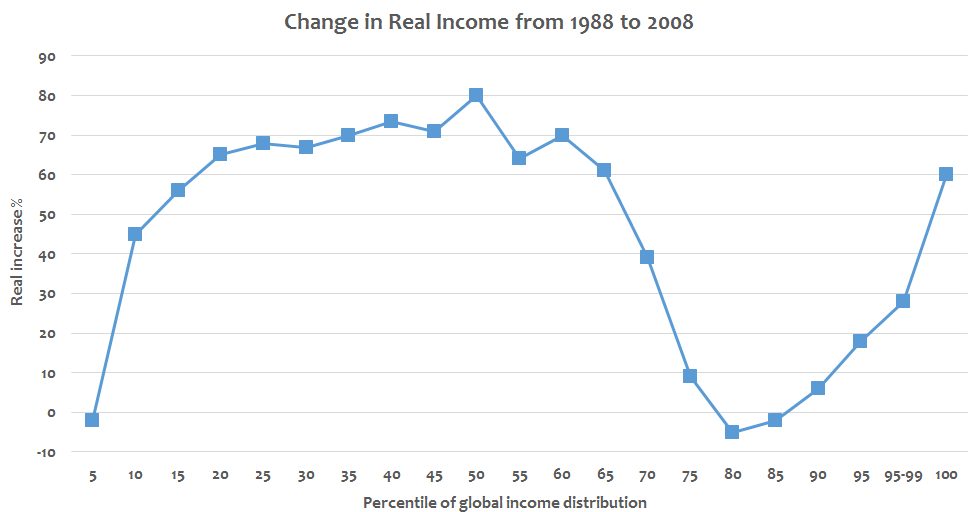
\includegraphics[width=\textwidth]{elephant_chart.png}
    \caption{Elephant Chart}
    \label{fig:elephant_chart}
\end{figure}

这条曲线看起来像一头大象:
\begin{itemize}
\item \textbf{象鼻高高翘起:} 全球收入最高的1\%(全球精英),他们的收入增长了超过60\%。他们是全球化的最大赢家。
\item \textbf{象背高高隆起:} 位于全球收入中段的人群,主要是以中国为代表的新兴经济体的中产阶级,他们的收入实现了惊人的增长,很多人实现了翻番甚至更多。这是全球化最值得称道的成就——数亿人脱离了贫困。
\item \textbf{象鼻与象背之间的低谷:} 位于全球收入分配高端(大约75-90百分位)的人群,他们的收入增长几乎为零,甚至为负。这部分人,恰恰就是\textbf{发达国家的下层和中产阶级}。
\end{itemize}

“大象曲线”清晰地告诉我们:全球化的果实,被全球最富有的那一小撮人和发展中国家的新兴中产阶级所分享,而发达国家的普通劳动者,则成了被遗忘的“输家”。

\item \textbf{发达国家内部的两极分化}
在美国等发达国家,CEO的薪酬与普通员工的薪酬差距,从几十倍拉大到几百倍。资本的回报率(利息、股息、资本利得)持续高于劳动回报率(工资),这是法国经济学家托马斯·皮凯蒂(Thomas Piketty)在《21世纪资本论》中揭示的核心趋势。全球化加剧了这一趋势:资本可以全球流动避税,而劳动力则基本被困在原地。工会力量因企业可以轻易将工厂外迁的威胁而被削弱,政府也不敢对资本和富人征收重税,担心他们会“逃离”。

\item \textbf{发展中国家内部的撕裂}
即使是在作为“赢家”的发展中国家,全球化也带来了内部的巨大撕裂。少数与全球市场接轨的精英、出口导向型企业主和生活在沿海大城市的人群迅速暴富,而广大的内陆地区、农村人口和传统产业的从业者,则可能被边缘化。中国的城乡差距、印度的阶级固化,都在全球化时代被进一步拉大。
\end{itemize}

当一个社会大部分的经济增长果实只被少数人攫取,当社会流动性下降,普通人无论如何努力都无法改善生活时,社会的公平感和正义感就会被侵蚀,对现有政治经济体制的愤怒和不信任感就会滋生,为民粹主义和激进政治的兴起提供了最肥沃的土壤。

\subsection{文化认同的冲击:我是谁?我们是谁?}

全球化不仅是商品和资本的流动,也是文化、价值观和生活方式的流动。这种流动在促进交流的同时,也引发了深刻的文化焦虑和认同危机。

\begin{itemize}
\item \textbf{“文化帝国主义”的担忧}
以好莱坞、麦当劳、星巴克为代表的西方消费文化,随着全球化席卷全球。这在一些国家引发了对“文化帝国主义”的担忧,认为本土的文化传统、语言和价值观正在被同质化的、强势的西方文化所侵蚀。
\begin{itemize}
\item \textbf{案例:法国的“文化例外”}
法国长期以来都奉行“文化例外”(l'exception culturelle)政策,坚称文化产品不是普通商品,不能完全遵循自由贸易原则。为了抵御好莱坞的冲击,法国政府通过补贴、税收优惠和规定电台必须播放一定比例的法语歌曲、影院必须排映一定比例的法国电影等方式,来保护和扶持本国的文化产业。这正是对文化全球化的一种自觉抵制。
\end{itemize}

\item \textbf{移民带来的社会张力}
全球化带来的人员流动,尤其是大规模的移民,深刻地改变了许多西方社会的人口结构。虽然移民为社会带来了劳动力和多样性,但也引发了关于资源分配、社会融合和国家认同的激烈争论。
\begin{itemize}
\item \textbf{案例:欧洲的移民危机与右翼崛起}
2015年,大量来自中东和北非的难民涌入欧洲,引发了严重的社会和政治危机。在许多欧洲民众看来,大规模的、文化背景迥异的移民,不仅对本国的福利体系、社会治安构成了压力,更重要的是,它挑战了“我们是谁”这个根本问题。德国的“我们能做到”(Wir schaffen das)的开放政策,与匈牙利等国修建边境墙的强硬做法,形成了鲜明对比。
欧洲各国的右翼民粹政党,如法国的国民联盟、德国的选择党,正是利用了民众的这种不安和恐惧。他们将移民问题与恐怖主义、失业和文化丧失等问题捆绑在一起,将自己塑造为“本土文化”和“国家认同”的捍卫者,从而获得了大量选票。
\end{itemize}

\item \textbf{“全球化主义者” vs. “本土主义者”}
英国学者戴维·古德哈特(David Goodhart)提出了一个极具解释力的概念框架,他将社会分为了两类人:“无根的全球化主义者”(Anywheres)和“有根的本土主义者”(Somewheres)。
\begin{itemize}
\item \textbf{Anywheres(世界公民):} 他们通常受过高等教育,从事专业性工作,流动性强,视野全球化。他们从全球化中受益,认同开放、多元、包容的普世价值。他们感觉自己既可以属于伦敦,也可以属于纽约或上海。
\item \textbf{Somewheres(本土居民):} 他们是社会的大多数,受教育程度相对较低,生活和工作与特定的“地方”(家乡、社区)紧密相连。他们的身份认同根植于本土的传统、文化和社群关系。他们感觉被全球化浪潮所抛弃和威胁,他们的价值观(如家庭、宗教、国家)被“Anywheres”所鄙视。
\end{itemize}
\end{itemize}

脱欧公投和特朗普的当选,在很大程度上可以被看作是人数众多的“Somewheres”对人数较少但掌控话语权的“Anywheres”的一场政治反叛。这解释了为什么许多投票支持脱欧或特朗普的地区,恰恰是那些经济上受全球化冲击最严重、同时在文化上感觉被忽视的地区。

\section{全球化的赢家与输家:一幅残酷的众生相}

综合以上分析,我们可以清晰地勾勒出全球化这场盛宴中的“赢家”与“输家”。它从来不是一场普惠所有人的派对,而是一场深刻的利益重分配。

\begin{itemize}
\item \textbf{主要赢家:}
\begin{itemize}
\item \textbf{跨国公司及其高管/股东:} 他们是全球化的总设计师和最大受益者。通过全球布局,他们实现了成本最小化和利润最大化。
\item \textbf{全球金融精英:} 华尔街的银行家、基金经理们,通过资本的全球自由流动,创造和积累了惊人的财富。
\item \textbf{发达国家的高技能专业人士:} 硅谷的工程师、律师、顾问等“知识工人”,他们的技能在全球市场中具有稀缺性,因而获得了高额回报。
\item \textbf{成功融入全球产业链的发展中国家(及其部分国民):} 以中国、越南等为代表的国家,通过承接制造业转移,实现了经济的飞速增长,创造了庞大的新兴中产阶级,数亿人摆脱了绝对贫困。这是全球化最积极、最不可否认的成就。
\item \textbf{全球消费者(在一定程度上):} 享受到了来自世界各地的、前所未有地廉价和多样化的商品。
\end{itemize}

\item \textbf{主要输家:}
\begin{itemize}
\item \textbf{发达国家的蓝领工人和低技能劳动者:} 他们是全球化最直接的受害者,面临失业、工资停滞和职业尊严的丧失。
\item \textbf{未能融入全球经济的发展中国家(及其大部分国民):} 许多非洲和拉美的国家,在全球化中被进一步边缘化。它们没有强大的制造业基础,只能出口初级原材料,在全球分工中处于最底层,国内贫困问题依然严峻。
\item \textbf{受冲击的本土中小企业:} 它们无力与拥有巨大规模和成本优势的跨国公司竞争,在本国市场也面临被挤压的困境。
\item \textbf{地球环境:} 全球生产和消费的极大扩张,以及廉价的跨国运输,加剧了碳排放、资源消耗和环境污染。污染密集型产业从监管严格的发达国家转移到监管宽松的发展中国家,形成了“污染天堂”。
\end{itemize}
\end{itemize}

当“输家”群体的数量和怨气积累到一定程度,并且他们的声音能够通过民粹主义政治家被有效动员起来时,“逆全球化”的浪潮便不可避免地到来了。

\section{逆全球化浪潮:表现、动因与未来}

当前的“逆全球化”浪潮,并非要让世界退回到各国老死不相往来的孤立状态,这在技术上和经济上都已不可能。它更像是一次对过去三十年“超全球化”模式的激烈修正和重塑。

\begin{itemize}
\item \textbf{主要表现:}
\begin{itemize}
\item \textbf{贸易保护主义抬头:} 最典型的就是特朗普政府发动的对华贸易战,大规模加征关税。但这种做法并非美国独有,印度、巴西等国也在提高关税,欧盟则通过“碳边境调节机制”(CBAM,即碳关税)等新型贸易壁垒来保护自身产业。
\item \textbf{供应链的“去风险化”与“区域化”:} COVID-19疫情暴露了全球供应链的脆弱性——当某个环节(如中国的港口)中断,全球生产都可能陷入停滞。俄乌冲突则让各国意识到将供应链过度集中于“地缘政治对手”的风险。因此,各国政府和企业开始推动供应链的调整,从过去单纯追求“效率”转向追求“安全”和“韧性”。
\begin{itemize}
\item \textbf{近岸外包(Near-shoring):} 将生产线从遥远的亚洲迁回离本国更近的地区(如美国公司迁往墨西哥)。
\item \textbf{友岸外包(Friend-shoring):} 将供应链集中在政治上可信赖的盟友国家。
\item \textbf{产业政策回归:} 各国政府不再羞于谈论“产业政策”,而是通过巨额补贴来扶持本国的关键产业,如美国的《芯片与科学法案》和《通胀削减法案》,旨在将半导体和新能源产业吸引回本土。
\end{itemize}
\item \textbf{民族主义和民粹主义政治的常态化:} “本国优先”的口号在全球范围内流行。政治家们通过煽动排外情绪、强调国家利益至上,来获取国内政治支持。
\item \textbf{全球合作的困境:} 在气候变化、公共卫生、核不扩散等亟需全球合作的领域,大国间的战略竞争和不信任感,使得达成和执行有意义的国际协议变得异常困难。
\end{itemize}

\item \textbf{未来展望:一个“有管理的全球化”?}
未来的全球化,可能不再是过去那种野蛮生长的、无限制的自由流动。它可能会呈现出以下几个特征:
\begin{enumerate}
\item \textbf{更具选择性:} 国家会在数字、金融等领域保持开放,但在涉及国家安全和关键技术的领域,则会加强保护和管制。
\item \textbf{更加区域化:} 以欧盟、北美(USMCA)、东亚(RCEP)为核心的三大区域经济集团的内部联系会更加紧密,而跨区域的联系则可能面临更多障碍。
\item \textbf{更加注重公平与安全:} 国内的公平分配问题(如何补偿全球化中的输家)和供应链的安全问题,将被置于比单纯追求经济效率更优先的位置。
\item \textbf{更加政治化:} 经济决策将越来越多地服务于地缘政治目标,国家安全考量将深刻影响贸易和投资的流向。
\end{enumerate}
\end{itemize}

\section{结论:在断裂的世界中重新思考连接}

全球化,这把曾经被认为是能斩断贫困与冲突的“利剑”,终究显露了它的“双刃”本质。它在连接世界、创造财富的同时,也切断了许多人与稳定工作、与家乡社区、与传统认同之间的纽带。它带来的巨大经济收益,与它造成的深刻政治创伤,共同构成了我们这个时代的复杂面貌。

“逆全球化”的浪潮,正是这些被全球化叙事所忽视、所压抑的政治创伤的总爆发。它是对主权流失的焦虑、对经济不公的愤怒、对文化失落的恐慌的集体回应。它提醒我们,任何经济模式如果不能在政治上和社会上获得持续的合法性,终将是不可持续的。

理解了全球化如何通过冲击经济和主权来催生政治反抗,我们便能更好地把握当今世界政治的核心矛盾。然而,故事还未结束。当这些由全球化带来的经济和文化上的不安全感,与一个社会内部早已存在的、更深层次的身份裂痕——如种族、宗教、地域——相互交织时,又会引爆怎样更具破坏性的政治能量?为什么在许多国家,政治辩论的核心已经从“我们应该做什么”(政策),变成了“我们是谁”(身份)?为什么“你来自哪里”似乎比“你是谁”更加重要?

这,正是我们下一章将要深入探讨的,当代政治的另一个幽灵——“身份政治”。
\part{政治的动态——冲突与参与}

\chapter{为什么“你来自哪里”有时比“你是谁”更重要?——深入解读身份政治的浪潮}

想象一下这个场景:一场激烈的总统大选辩论中,候选人没有在争论税率高低或福利政策的细节,而是在激烈地讨论一个历史人物的雕像是否应该被推倒。或者,在另一个国家,选举的结果并非取决于经济纲领的优劣,而是几乎完全由选民的民族或宗教归属所决定。在社交媒体上,人们因为对某个社会事件的看法不同而迅速站队,用“觉醒”(Woke)或“顽固”(Bigot)等标签互相攻击,仿佛彼此生活在完全不同的现实中。

这些看似孤立的现象,背后都指向一个共同的、正在深刻重塑全球政治版图的力量——\textbf{身份政治(Identity Politics)}。

在上一章中,我们探讨了全球化这把“双刃剑”如何催生了“逆全球化”的浪潮。当全球化带来的经济冲击与社会内部早已存在的裂痕相遇时,一种比经济阶级更古老、更具情感煽动性的力量便被唤醒了。在现代政治的舞台上,我们越来越频繁地目睹一个令人深思的现象:在许多国家,一个人的政治立场、社会归属感乃至人生机遇,似乎更多地由其所属的群体身份(如种族、民族、宗教、性别、性取向等)所决定,而非其个人的品格、才能或奋斗。

这种“你来自哪里”(你的群体归属)压倒“你是谁”(你的个体价值)的趋势,正是身份政治的核心。它像一个巨大的磁场,将社会中的个体吸附到不同的“部落”中,并以“我们”和“他们”的视角重新定义政治斗争。这不禁让人好奇:为什么在物质生活空前丰富的今天,这些看似前现代的身份认同,反而成为了如此强大的政治动员力量?它与我们熟悉的、以经济利益为核心的阶级政治,究竟是何种关系?它是在弥合社会不公,还是在撕裂社会共识?

本章将带领读者踏上一场思想的深度探索之旅。我们将不仅仅满足于给身份政治下一个定义,更要通过一系列来自全球各地的、生动而深刻的案例,去解剖它的起源,探究它兴起的深层原因,并厘清它与阶级政治之间复杂而微妙的互动。这趟旅程将帮助我们理解,为何在21世纪的今天,身份的旗帜会在世界各地被高高举起。

\section{ 什么是身份政治?——当“我们”成为一种力量}

从根本上说,“身份政治”是指\textbf{基于共同的群体身份而形成的政治联盟、动员和诉求}。这些身份可以多种多样,包括但不限于:
\begin{itemize}
    \item \textbf{种族与民族:} 如美国的非裔、拉丁裔,南非的祖鲁人,中国的少数民族等。
    \item \textbf{宗教:} 如印度的印度教徒与穆斯林,北爱尔兰的天主教徒与新教徒。
    \item \textbf{性别与性取向:} 如全球的女权运动(\#MeToo),LGBTQ+平权运动。
    \item \textbf{地域与文化:} 如西班牙的加泰罗尼亚独立运动,加拿大的魁北克分离主义。
    \item \textbf{其他:} 如代际(婴儿潮一代 vs. Z世代)、残障状况、职业群体等。
\end{itemize}

身份政治的核心,是将一个群体的\textbf{共同经验},尤其是\textbf{受排斥、受歧视或被边缘化的历史与现实},转化为政治行动的燃料。它不再满足于传统政治中对“普遍公民权利”的模糊承诺,而是振臂高呼:“请看到我们的独特性!请承认我们遭受的不公!请给予我们应有的尊重和权利!”

\subsection{身份政治的三大核心特征}

为了更清晰地把握身份政治,我们可以将其拆解为三个相互关联的核心特征:

\begin{enumerate}
    \item \textbf{群体性(Group-Based):政治的“主语”从“我”变成了“我们”。}
    传统自由主义政治强调个体权利,认为国家应平等对待每一个独立的公民。而身份政治则认为,在现实世界中,个体往往是作为某个群体的成员而被社会所对待的。例如,一个黑人工程师在求职时,他所面临的隐性偏见可能与他的个人能力无关,而仅仅因为他的肤色。因此,要改变这种状况,不能仅靠他个人的奋斗,而需要整个非裔群体的集体发声和抗争。\textbf{Black Lives Matter(黑人的命也是命)}运动就是一个典型的例子。它并非宣称黑人的生命比其他人更重要,而是强调在美国的司法和执法体系中,黑人的生命长期被系统性地轻视,因此需要作为一个\textbf{特定群体}的议题被提出来,加以纠正。政治行动的主体,是“黑人”这个身份群体。

    \item \textbf{独特性(Specificity):强调“我们的故事”与众不同。}
    身份政治的核心情感动力,来自于对本群体独特历史经验和文化叙事的强调。它拒绝被“大熔炉”式的同化叙事所淹没,而是要大声讲出“我们的故事”。例如,澳大利亚原住民的政治诉求,不仅仅是要求经济补偿,更是要求国家承认他们作为这片土地最早主人的历史地位,承认殖民化给他们带来的文化断裂和世代创伤。他们的口号“Always Was, Always Will Be”(过去是,将来永远是)就体现了这种对独特历史身份的坚守。这种对独特性的强调,旨在挑战主流社会“一刀切”的政策和视角,要求制定更能回应特定群体需求的方案。

    \item \textbf{政治化(Politicization):将“私人”的痛苦转化为“公共”的议题。}
    身份政治最关键的一步,是将原本被认为是个人私事、家庭内部事务或社会文化层面的问题,提升到公共领域和政治议程上。20世纪60年代,第二波女权运动提出的口号\textbf{“个人即政治”(The Personal is Political)}完美地诠释了这一点。一个女性在家庭中遭遇的暴力,在职场上遇到的“玻璃天花板”,长期以来被视为“个人不幸”或“家庭矛盾”。但女权运动者指出,这并非孤立事件,而是由整个社会存在的、系统性的性别歧视(父权制)所造成的。因此,家庭暴力需要立法干预,同工同酬需要法律保障,女性的身体自主权(如堕胎权)需要成为国家必须回应的政治议题。通过这种方式,身份政治将无数个体的“私人痛苦”汇聚成强大的政治诉求,迫使政治体系做出回应。
\end{enumerate}

\subsection{历史的回响:身份政治的起源与演变}

身份政治并非凭空出现的新鲜事物,它的根源深植于人类历史的长河中。但其在20世纪中后期以来的集中爆发,则与特定的历史背景密切相关。

\textbf{西方社会的“权利革命”:}

20世纪60年代是西方身份政治的“引爆点”。此前,主流政治主要围绕经济阶级(劳工 vs. 资本家)和意识形态(共产主义 vs. 资本主义)展开。但随着战后经济的繁荣和“冷战”格局的稳定,一些被经济议题所掩盖的社会矛盾开始凸显。
\begin{itemize}
    \item \textbf{美国民权运动(1950s-1960s):} 这是现代身份政治的典范。以马丁·路德·金为代表的非裔美国人,通过“非暴力抵抗”的方式,如蒙哥马利公交车抵制运动、华盛顿大游行等,挑战南方的种族隔离制度。他们诉求的不仅仅是经济地位的改善,更是作为“人”的基本尊严和作为“美国公民”的平等权利。这场运动最终催生了《1964年民权法案》和《1965年选举权法案》,从法律上终结了种族隔离,成为身份政治通过集体行动改变国家制度的成功范例。
    \item \textbf{第二波女权运动(1960s-1980s):} 受到民权运动的启发,女性开始挑战社会中无所不在的性别歧视。贝蒂·弗里丹的《女性的奥秘》揭示了家庭主妇们光鲜生活下的精神空虚,点燃了运动的火焰。她们争取教育平权、工作机会、同工同酬,并首次将堕胎权、性骚扰等议题带入公共视野。
    \item \textbf{石墙暴动与LGBTQ+权利运动(1969-至今):} 1969年,纽约“石墙酒吧”的同性恋群体对警方的歧视性搜捕发起了暴力反抗,这被视为现代同性恋权利运动的开端。从此,同性恋群体不再将自己的性取向视为需要隐藏的“疾病”或“罪恶”,而是作为一种值得骄傲的身份,公开要求社会承认和法律保护。从反歧视立法到争取同性婚姻合法化,这场运动至今仍在全球范围内推进。
\end{itemize}

\textbf{非西方世界的遗产与抗争:}

在许多非西方国家,身份政治的根源更为古老和复杂,常常与殖民主义、国家构建和内部族群关系紧密相连。
\begin{itemize}
    \item \textbf{后殖民时代的民族主义:} 在亚非拉地区,反抗殖民统治的斗争本身就是一场声势浩大的身份政治运动。被殖民者以“民族”的身份团结起来,反抗宗主国的压迫。然而,独立之后,殖民者当初为了“分而治之”而划定的人为边界,以及他们对某些族群的扶持或打压,往往给新生的国家埋下了冲突的种子。
    \item \textbf{案例:卢旺达的悲剧——被制造的身份。} 在殖民前,胡图族(Hutu)和图西族(Tutsi)更多是社会阶层的划分,可以相互转化。但比利时殖民者为了便于统治,发放了标明种族的身份证,并长期扶持占少数的图西族精英。这种人为固化的身份划分,加剧了族群间的隔阂与怨恨。1994年,当政治精英为了巩固权力而煽动种族仇恨时,这种被强化的身份认同最终引爆了惨绝人寰的种族大屠杀。这个案例极端地说明,身份并非总是天然的,它也可以被政治力量所“\textbf{建构}”和“\textbf{操纵}”,并带来毁灭性后果。
    \item \textbf{案例:印度的种姓政治——千年不变的烙印。} 印度的种姓制度是一种延续千年的、基于血缘的社会等级体系。尽管印度宪法早已废除“不可接触制”(贱民制度),但种姓身份在社会生活,尤其是在农村地区和婚配、就业等方面,依然影响深远。在政治上,以“达利特”(Dalit,即过去的“贱民”)为代表的低种姓群体,组建了自己的政党,如“大众社会党”(BSP),通过选票来争取教育配额、政府职位和政治权力,以对抗延续至今的结构性歧视。这是一种典型的、旨在颠覆古老等级秩序的身份政治。
\end{itemize}

\subsection{身份政治 vs. 阶级政治:一场范式的转移?}

传统政治分析,尤其是马克思主义理论,习惯于用“阶级”的透镜来观察世界。它认为,社会最根本的矛盾是基于经济地位的矛盾,即拥有生产资料的\textbf{资产阶级}和出卖劳动力的\textbf{无产阶级}之间的斗争。政治的核心议题是\textbf{经济再分配},目标是实现一个没有阶级压迫的、经济上平等的社会。

身份政治的兴起,则提供了一个不同的分析视角。它认为,压迫和不公不仅仅发生在经济领域,也深刻地存在于文化、社会和历史层面。一个富有的黑人企业家,可能依然会因为肤色而受到歧视;一个中产阶级的女性,可能依然会在职场上遭遇性别天花板。这些并非阶级问题,而是身份问题。

\begin{tabular}{|l|l|l|}
\hline
\textbf{维度} & \textbf{传统阶级政治} & \textbf{身份政治} \\
\hline
\textbf{核心矛盾} & 经济剥削(\textbf{资产阶级} vs. \textbf{无产阶级}) & 文化/社会排斥(\textbf{主流群体} vs. \textbf{边缘群体}) \\
\hline
\textbf{分析单位} & \textbf{经济阶级} & \textbf{身份群体}(种族、性别、宗教等) \\
\hline
\textbf{核心诉求} & \textbf{经济再分配}(财富、资源) & \textbf{承认与尊重}(文化、权利、尊严) \\
\hline
\textbf{斗争目标} & 消除阶级压迫,实现经济平等 & 消除身份歧视,实现多元共存 \\
\hline
\textbf{典型口号} & “全世界无产者,联合起来!” & “黑人的命也是命”、“个人即政治” \\
\hline
\end{tabular}

当然,这并不意味着身份政治已经完全取代了阶级政治。更准确地说,是政治斗争的“主战场”发生了部分转移,或者说,变得更加复杂了。人们开始意识到,一个人的社会处境,往往是阶级和身份双重因素叠加的结果。我们将在第三部分详细探讨这两者之间复杂的互动关系。

\section{ 身份的旗帜为何高高飘扬?——探寻身份政治的崛起根源}

为什么在21世纪,这个本应更加理性、开放和全球化的时代,身份的旗帜反而会在世界各地被越举越高?这并非偶然,而是多种深层力量交织作用的结果。我们可以从历史、经济、文化、政治和科技五个维度来解剖这一现象。

\subsection{根源一:历史的幽灵——未愈合的创伤与未竟的斗争}

许多身份群体的政治动员,本质上是对历史不公的迟来反应。历史并非一本尘封的旧书,它是一个活生生的幽灵,其留下的创伤和结构性不公,依然在塑造着今天的社会现实。
\begin{itemize}
    \item \textbf{案例:南非的后种族隔离时代。} 从1948年到1994年,南非实行了残酷的种族隔离(Apartheid)制度。白人少数政府通过法律,系统性地剥夺了黑人等非白人种族的土地、教育、工作机会和政治权利。尽管曼德拉领导的“\textbf{非国大}”(ANC)在1994年赢得了大选,结束了种族隔离,但历史的伤疤远未愈合。今天南非的政治辩论,依然频繁地围绕着“土地改革”(将白人农场主的土地重新分配给黑人)、“黑人经济赋权法案”(BEE, 要求企业有一定比例的黑人股份和高管)等议题展开。这些政策的争议性极强,但它们都源于一个共同的逻辑:必须通过今天的政治和经济手段,来纠正昨天的历史错误。对黑人民众而言,这不仅是经济问题,更是恢复种族尊严和实现真正解放的未竟事业。

    \item \textbf{案例:加拿大与原住民的“和解”之路。} 从19世纪末到20世纪末,加拿大政府强制将超过15万名原住民儿童送入“寄宿学校”,旨在强行同化他们,消除其语言和文化。这些学校虐待、性侵和疾病泛滥,造成了数千名儿童死亡和难以估量的代际创伤。近年来,随着这些历史被揭露,原住民的身份政治运动愈发高涨。他们要求政府的不仅仅是道歉和赔偿,更是对他们土地权、自治权和文化权的承认。2021年,多地寄宿学校旧址发现大量无名儿童坟墓,引发全国震动,也让原住民的诉求获得了前所未有的道义力量。这表明,只要历史的创伤没有被正视和疗愈,它就会持续为身份政治提供燃料。
\end{itemize}

\subsection{根源二:经济的裂痕——当不平等戴上身份的面具}

全球化和新自由主义经济政策在创造巨大财富的同时,也加剧了贫富分化。当经济上的不安全感和被剥夺感,与特定的身份群体高度重合时,身份认同就成了表达经济诉求和寻找“替罪羊”的天然载体。
\begin{itemize}
    \item \textbf{案例:美国“铁锈带”的白人身份政治。} 美国的“铁锈带”(Rust Belt)地区,曾是制造业中心。但在全球化浪潮中,大量工厂外迁,导致了大规模的失业和社区衰败。受影响最严重的是当地的白人蓝领阶层。他们感到被精英阶层所抛弃,生活水平下降,社会地位旁落。这种经济上的失落感,与一种文化上的焦虑感交织在一起:他们感到自己所代表的“传统美国”正在被移民、多元文化和“政治正确”所侵蚀。唐纳德·特朗普在2016年的崛起,精准地捕捉并利用了这种情绪。他的“让美国再次伟大”(Make America Great Again)口号,以及对移民和全球化的强硬立场,实际上是将复杂的经济问题,转化为了一个简单明了的身份叙事——“\textbf{我们}”(勤劳的、被遗忘的白人爱国者)对抗“\textbf{他们}”(抢走我们工作的移民、出卖国家利益的全球主义精英)。这是一种典型的、由经济焦虑催生的多数族群身份政治。

    \item \textbf{案例:马来西亚的“Bumiputera”政策。} 马来西亚是一个多民族国家,主要由马来人、华人和印度人组成。在英国殖民时期和独立初期,华人在经济上占据主导地位。为了解决马来人的经济弱势地位和缓和族群矛盾,政府于1971年开始推行“新经济政策”,其核心是“\textbf{Bumiputera}”(“土地之子”,特指马来人及原住民)优先政策。该政策在教育、就业、商业许可、购房等方面给予马来人系统性优待。这一政策在一定程度上提升了马来人的经济地位,但也深刻地将国家政治与族群身份捆绑在一起。选举变成了族群间的资源争夺战,任何试图挑战该政策的尝试都会被视为对马来人身份和权益的攻击。经济不平等问题,被彻底“\textbf{身份化}”了。
\end{itemize}

\subsection{根源三:文化的焦虑——在全球化的浪潮中寻找归属}

全球化、大规模移民和信息技术的发展,打破了地域的隔阂,让不同文化、宗教和价值观的群体前所未有地紧密接触。这种接触在促进交流与融合的同时,也可能引发强烈的文化冲击和认同焦虑。当人们感到自己熟悉的生活方式、传统价值观或宗教信仰受到“外来者”的威胁时,强化自身群体的身份认同,就成了一种寻求安全感和确定性的本能反应。
\begin{itemize}
    \item \textbf{案例:欧洲的穆斯林移民与世俗主义的冲突。} 以法国为例,其立国之本是严格的“\textbf{世俗主义}”(Laïcité)原则,强调在公共领域中完全消除宗教符号。然而,随着大量来自北非的穆斯林移民涌入,伊斯兰文化(如女性佩戴头巾)与法国的世俗传统发生了激烈碰撞。2004年,法国立法禁止在公立学校佩戴包括头巾在内的“明显的宗教标志”,2010年又立法禁止在公共场所穿戴遮盖全脸的罩袍(如尼卡布)。支持者认为这是在捍卫法国的共和价值观和解放女性,而许多穆斯林则认为这是对他们宗教自由和文化身份的公然歧视。这场“头巾战争”背后,是两种不同文明和价值观的冲突,它极大地强化了法国穆斯林群体的身份认同,也催生了反移民、捍卫“法兰西特性”的右翼身份政治。

    \item \textbf{案例:印度的“印度教民族主义”(Hindutva)崛起。} 印度是一个世俗国家,但印度教徒占人口的绝大多数。近年来,以现任总理莫迪领导的“印度人民党”(BJP)为代表的印度教民族主义势力迅速崛起。他们宣扬一种“\textbf{Hindutva}”思想,认为印度的国家认同应根植于印度教文化。他们将穆斯林等少数群体描绘为“外来者”或“潜在的威胁”,通过修建罗摩神庙、修改公民身份法案(被指歧视穆斯林)等行动,来动员和巩固印度教徒的身份认同。这种政治策略的成功,反映了在全球化时代,许多人渴望回归一种“纯粹”的、本土的文化身份,以抵御外部世界的变化和不确定性。
\end{itemize}

\subsection{根源四:精英的博弈——身份,一张最好打的政治牌}

在许多情况下,身份政治的兴起并非完全是自下而上的民众运动,政治精英的煽动和利用起到了至关重要的作用。相比于复杂的经济政策,身份认同的议题更具情感煽动性,更容易划分“我们”和“他们”,是动员选民、巩固权力的廉价而高效的工具。
\begin{itemize}
    \item \textbf{案例:前南斯拉夫的解体。} 在铁托的威权统治下,南斯拉夫各民族(塞尔维亚人、克罗地亚人、波斯尼亚人等)的矛盾被强力压制。但铁托去世后,经济危机和政治真空为民族主义野心家提供了舞台。斯洛博丹·米洛舍维奇等政治领袖,通过不断地挑动塞尔维亚人的“大国情怀”和对其他民族的历史积怨,将自己塑造为民族利益的捍卫者,从而攫取了巨大的政治权力。其他民族的政治精英也纷纷效仿,最终导致了曾经的“兄弟国家”陷入血腥的内战。南斯拉夫的悲剧警示我们,当政治精英选择打“身份牌”时,其破坏力是何等巨大。

    \item \textbf{民粹主义的全球浪潮:} 近年来全球范围内的民粹主义浪潮,其核心动员策略就是身份政治。无论是美国的特朗普、巴西的博索纳罗,还是匈牙利的欧尔班,他们都擅长将自己定位为“沉默的大多数”或“真正的人民”的代言人,并将国内的种种问题归咎于一小撮“腐败的精英”和“危险的少数群体”(如移民、少数族裔、LGBTQ+群体等)。通过这种方式,他们成功地将复杂的社会矛盾简化为一场身份对决,从而绕开了棘手的政策辩论。
\end{itemize}

\subsection{根源五:科技的赋能——算法编织的“部落”与回音室}

互联网和社交媒体的普及,为身份政治的兴起提供了前所未有的技术支持。它极大地改变了人们形成认同、组织动员和看待世界的方式。
\begin{itemize}
    \item \textbf{加速的组织与动员:} 在前互联网时代,组织一场大规模的社会运动需要耗费巨大的人力物力。而今天,一个标签(hashtag)就能引爆一场全球运动。\textbf{\#MeToo}运动就是最好的例子。2017年,一条推文引发了全球数百万女性在社交媒体上分享自己被性骚扰和性侵犯的经历。社交媒体为长期处于沉默和孤立状态的受害者提供了一个安全的公共空间,让她们发现“\textbf{我不是一个人}”。这种瞬间形成的集体认同感,迅速转化为强大的政治压力,导致许多有权势的男性倒台,并推动了全球范围内对职场性骚扰问题的反思和立法。

    \item \textbf{信息茧房与回音室效应:} 社交媒体的推荐算法,倾向于向用户推送他们感兴趣或认同的内容,这会形成“\textbf{信息茧房}”(Filter Bubble),让人们越来越难以接触到不同的观点。同时,在同一个身份群体的社交网络中,相同的观点被反复强调和肯定,形成“\textbf{回音室效应}”(Echo Chamber)。这会不断强化群体内部的认同感和对外部世界的偏见,使得不同群体之间的对话变得异常困难,社会共识的基础被侵蚀,政治极化加剧。例如,在关于疫苗、气候变化或特定政治事件的讨论中,支持和反对的阵营仿佛生活在两个平行的宇宙,各自消费着完全不同的“事实”和“真相”,这背后就有算法的推波助澜。
\end{itemize}

\section{ 当身份遇上阶级:当代政治的十字路口}

身份政治的兴起,并不意味着传统阶级政治的终结。在现实世界中,这两股强大的力量常常以一种复杂、动态甚至矛盾的方式相互作用,共同塑造着我们这个时代的政治图景。理解它们之间的关系,是看清当代社会纷繁乱象的关键。

\subsection{关系一:相互交织——“交叉性”的视角}

身份和阶级并非两个互不相干的标签,而是像DNA双螺旋一样,紧密地缠绕在一起,共同决定了个体在社会结构中的位置。美国黑人女性法学家金伯利·克伦肖(Kimberlé Crenshaw)在1989年提出了一个极具影响力的概念——\textbf{“交叉性”(Intersectionality)}。

“交叉性”理论指出,个体所承受的压迫和歧视,往往是多种身份(如种族、性别、阶级、性取向等)交叉作用的结果。我们不能孤立地看待其中任何一个维度。
\begin{itemize}
    \item \textbf{案例:一个贫穷的黑人女性。} 她的生活困境,不能简单地归结为“阶级问题”(因为贫穷的白人男性不会面临种族歧视),也不能简单地归结为“种族问题”(因为富有的黑人男性不会面临性别歧视和贫困的压力),更不能简单地归结为“性别问题”(因为贫穷的白人女性不会面临种族歧视)。她所面临的,是\textbf{贫穷、黑人和女性}这三重身份叠加所带来的、独特的、复合式的社会劣势。她在就业市场上可能既要面对种族偏见,又要面对性别偏见,还要承受低薪工作的剥削。
\end{itemize}

“交叉性”的视角告诉我们,身份政治和阶级政治的诉求在很多时候是高度重叠的。例如,为美国拉丁裔农场工人争取更高的工资和更好的劳动条件,这既是一场\textbf{阶级斗争}(劳工权利),也是一场\textbf{身份斗争}(反对针对少数族裔的剥削)。成功的政治运动,往往需要同时回应这两个层面的诉求。只谈阶级不谈种族,会忽视白人劳工和有色人种劳工所面临的不同挑战;反之,只谈种族不谈阶级,则可能掩盖精英阶层与底层民众在任何族群内部都存在的深刻矛盾。

\subsection{关系二:相互替代——当身份的战鼓压过阶级的呐喊}

在某些特定的历史和社会条件下,身份政治的激烈程度会完全压倒阶级政治,成为社会动员和政治分野的唯一主轴。在这种情况下,身份认同的“磁力”是如此之强,以至于来自不同阶级的同一个身份群体成员(例如,富有的和贫穷的胡图人)会团结起来,对抗另一个身份群体。
\begin{itemize}
    \item \textbf{案例:北爱尔兰的“麻烦”(The Troubles)。} 从20世纪60年代末到90年代末,北爱尔兰经历了长达三十年的暴力冲突。这场冲突的对阵双方,一方是希望北爱尔兰脱离英国、与爱尔兰统一的\textbf{天主教徒/民族主义者},另一方则是希望继续留在英国的\textbf{新教徒/联合主义者}。尽管双方内部都有富人和穷人,有资本家和工人,但在残酷的教派冲突面前,阶级差异变得无足轻重。一个天主教工厂主和一个天主教工人,在政治上会坚定地站在一起,对抗新教徒。政治、社会生活甚至居住区域,都按照教派身份被严格划分。在这里,宗教/民族身份彻底\textbf{替代}了阶级,成为了定义一切政治冲突的根本逻辑。

    \item \textbf{案例:印度-巴基斯坦分治。} 1947年,英属印度在独立时被分割为以印度教徒为主的印度和以穆斯林为主的巴基斯坦。这场“印巴分治”是20世纪最大规模的身份政治实践,它基于一个简单的逻辑:宗教身份是构建国家的首要原则。分治引发了人类历史上罕见的宗教仇杀和人口大迁徙,上千万人流离失所,上百万人死于非命。穆斯林地主和穆斯林农民一起逃往巴基斯坦,印度教商人和印度教“贱民”则一起逃往印度。在宗教身份的生死抉择面前,阶级团结的理想不堪一击。
\end{itemize}

\subsection{关系三:相互竞争与补充——左翼政党的困境与策略}

在许多西方民主国家,身份政治与阶级政治的关系更多表现为一种在政治议程上的\textbf{竞争与补充},这尤其体现在传统左翼政党的内部张力中。

传统上,左翼政党(如社会党、工党)的根基是工人阶级,其核心议程是经济再分配、社会福利和劳工权利。然而,随着20世纪后半叶身份政治运动的兴起,这些政党开始越来越多地吸纳和代表少数族裔、女性、LGBTQ+群体等身份群体的诉求。这就带来了一个深刻的困境:\textbf{如何在有限的政治议程中,平衡阶级议题和身份议题?}
\begin{itemize}
    \item \textbf{挑战与竞争:} 一些批评者,如美国政治学者马克·里拉(Mark Lilla),认为当代左翼政党(如美国的民主党)过于沉迷于“\textbf{身份自由主义}”(identity liberalism),将过多的精力放在了满足不同身份群体的“承认”诉求上,而忽视了能够团结大多数人的、普遍性的经济议题。这种“部落化”的政治策略,使得他们疏远了曾经的核心票仓——白人蓝领阶级,从而在选举中将他们推向了右翼民粹主义的怀抱。从这个角度看,对身份政治的过度关注,\textbf{削弱}了阶级政治的动员能力,导致了政治上的碎片化和失败。这种现象也被称为“\textbf{压迫的奥林匹克}”(Oppression Olympics),即不同身份群体之间相互竞争,比拼谁更受压迫,以争取优先的政治关注,从而破坏了更广泛的团结。

    \item \textbf{机遇与补充:} 另一些人则认为,身份政治是对传统阶级政治的必要\textbf{补充和深化}。它揭示了仅靠阶级分析无法解释的、深刻的社会不公。例如,推动性别平权和种族平等的政策,本身就是实现经济正义的重要组成部分,因为性别和种族恰恰是导致经济不平等的重要因素。一个成功的现代左翼政党,必须学会构建一个“\textbf{彩虹联盟}”,将不同身份群体的特殊诉求,与一个追求普遍经济公平的宏大愿景结合起来。例如,将争取“\textbf{同工同酬}”(性别议题)和提高“\textbf{最低工资}”(阶级议题)结合起来,共同服务于一个更大的社会正义目标。这要求政治家拥有高超的智慧,既要承认差异,又要寻求共识。
\end{itemize}

\section{ 结论:在身份的迷宫中,寻找未来的出口}

“你来自哪里”在今天许多国家比“你是谁”更重要,这一现象并非历史的倒退,而是当代社会矛盾在政治领域的一种复杂呈现。它如同一面棱镜,折射出历史遗留的伤痕、全球化带来的经济裂痕、不同文化间的价值碰撞、政治精英的策略博弈以及数字时代的技术冲击。

身份政治的兴起,是一柄锋利的双刃剑。

\textbf{从积极的方面看},它为那些在历史上长期被忽视、被压迫、被沉默的群体提供了发声的麦克风和抗争的旗帜。它推动了民权、女权、残障人士权利等一系列伟大的社会进步,极大地丰富了我们对“公正”和“平等”的理解。它迫使主流社会去直面那些不愿正视的阴暗角落,让一个更多元、更包容的社会成为了可能。从这个意义上说,身份政治是通往更深层次社会正义的必经之路。

\textbf{但从消极的方面看},当身份政治走向极端,它也会变成腐蚀社会信任、加剧政治极化的毒药。它可能将世界简化为“我们”与“他们”的永恒对立,将复杂的社会问题归咎于某个“替罪羊”群体,从而扼杀理性对话和妥协的可能。它可能导致社会“部落化”,让人们缩回到各自的身份壁垒中,用标签取代理解,用口号取代思考,最终撕裂国家凝聚力的根基。

理解身份政治的复杂性,及其与阶级政治的纠缠,对于我们把握当今世界的脉搏至关重要。它要求我们超越非黑即白的简单化思维,既要看到承认身份差异、纠正历史不公的必要性,也要警惕身份认同被滥用为煽动仇恨、分裂社会的工具。

我们正处在一个身份的迷宫之中。如何在这个迷宫中找到一条既能尊重个体差异,又能凝聚社会共识的出口?这考验着每一个现代社会的智慧和韧性。而当这些由身份和阶级矛盾所点燃的社会怒火无法在现有体制内得到疏解时,它们就可能汇聚成一股更为猛烈的力量,足以颠覆整个旧秩序——那就是革命。

那么,为什么旨在创造新世界的“革命”,常常会反过来“吃掉自己的孩子”,陷入暴力与混乱的循环?这正是我们下一章将要深入探讨的、更为残酷的政治现实。


\chapter{为什么“革命”不是请客吃饭,常常会“吃掉自己的孩子”?}

1794年4月5日,巴黎革命广场(即今天的协和广场)的断头台下,人声鼎沸。当法国大革命的巨人、曾经的“首席演说家”乔治·丹敦(Georges Danton)走上刑场时,他显得异常平静,甚至带着一丝傲慢。他先是安慰身边同样面临死亡的年轻朋友,然后转身对着刽子手,留下了那句被历史铭记的遗言:“别忘了把我的头给民众看,它是值得一看的。”片刻之后,刀刃落下,这位曾经用他雄辩的口才点燃了整个法兰西激情的革命领袖,最终被他亲手缔造的革命所吞噬。

丹敦的悲剧,并非孤例,甚至不是这场革命中最具讽刺意味的一幕。仅仅三个多月后,曾经将丹敦送上断头台的“不可腐蚀者”---马克西米连·罗伯斯庇尔(Maximilien Robespierre),这位恐怖统治的最高化身,同样被他的政治对手们送上了同一个断头台。据说,当他那被子弹击碎的下颚被草草包扎着押赴刑场时,广场上爆发出比处决丹敦时更为热烈的欢呼。

从罗伯斯庇尔到托洛茨基,从布哈林到刘少奇,历史上无数的革命者最终都倒在了自己同志的屠刀之下。在上一章中,我们探讨了身份政治的动员力量。当这种力量与社会深层矛盾结合,便可能引爆最具颠覆性的社会变革---革命。人类历史上,革命总是与“自由、平等、博爱”、“面包、和平、土地”这样激动人心的口号相伴,它承诺砸碎旧世界的锁链,建立一个崭新的、无限美好的未来。然而,历史的吊诡之处在于,追求天堂的努力,往往会通往地狱。许多革命在推翻旧秩序后,并未迎来承诺的乌托邦,反而陷入了更深的混乱、暴力与专制。这便是令人不寒而栗的“革命吃掉自己的孩子”(The revolution devours its own children)现象。

为什么一场以解放为名的运动,最终会走向奴役?为什么追求理想的革命者,会变成冷酷的独裁者?本章将深入革命的肌理,从其爆发的结构性根源,到其失控的动态过程,系统地剖析这一历史性的难题。我们将像法医一样,解剖“革命”这具复杂而迷人的“尸体”,探寻其内在的基因与病理。

\section{革命的解剖学:引爆社会火山的结构性裂痕}

“革命”(Revolution)并非简单的政权更迭或暴动,而是一场在短时间内,通过非常规乃至暴力的手段,对整个社会的政治制度、社会结构、权力关系和主流价值观进行的根本性、颠覆性的重塑。它不是茶壶里的风暴,而是社会深层矛盾的总爆发,如同地壳板块长期挤压后引发的剧烈地震。著名政治社会学家西达·斯考切波(Theda Skocpol)在她的经典著作《国家与社会革命》中,通过比较法国、俄国和中国的革命,发现伟大的社会革命并非由革命者“创造”的,而是特定结构性条件下的产物。革命的爆发,通常需要以下几个“结构性条件”同时在场。

\subsection{“利维坦”的倒下:国家能力的衰退与崩溃}

强大的国家机器是维持社会秩序的“压舱石”。然而,当这台机器锈迹斑斑、濒临瘫痪时,革命的机遇之窗便悄然打开。国家能力的衰退,主要体现在以下几个方面:
\begin{itemize}
\item \textbf{财政破产:这是最常见的导火索。} 当国家“钱袋子”空了,一切都无从谈起。一个无法支付军队薪水、官僚工资和公共服务的政府,其权威也就荡然无存。
    \begin{itemize}
    \item \textbf{案例:法国旧制度(Ancien Régime)的末日}
        18世纪末的法国,表面上是欧洲大陆的文化和政治中心,内部却已千疮百孔。国王路易十六的宫廷在凡尔赛宫夜夜笙歌,挥霍无度。更致命的是,为了与宿敌英国争霸,法国深度参与了“烧钱”的美国独立战争。这场战争虽然帮助美国赢得了独立,却也把法国的国库彻底打空。为了弥补高达数亿里弗的巨额赤字,政府唯一的办法就是加税。但法国的税收制度极不公平,享受着最多社会资源的贵族和教士阶级却享有免税特权,沉重的负担几乎全部压在了平民,尤其是农民和新兴的资产阶级身上。当财政总监们(如杜尔哥、内克)试图推动税收改革,触动特权阶级的利益时,无一例外地遭到强烈抵制而失败。一个无法公平有效汲取财政,也无法进行自我革新的国家,其统治基础已经被掏空。1789年,路易十六为解决财政问题而被迫召开的三级会议,最终成为了点燃革命的火柴。
    \item \textbf{案例:晚明王朝的财政崩溃}
        将目光转向东方,17世纪中叶的中国明朝,也上演了惊人相似的一幕。崇祯皇帝面临着“北有强敌(后金),内有流寇”的绝境,而国家的财政体系早已捉襟见肘。为了支撑辽东前线的军费和镇压国内农民起义的开销,明政府先后增加了“辽饷”、“剿饷”和“练饷”,史称“三饷加派”。这些沉重的税负,如雪上加霜,被层层转嫁到早已不堪重负的农民身上。更具讽刺意味的是,为了节省开支,崇祯还裁撤了全国的驿站。这一举措,直接导致一位名叫李自成的驿卒失业。这位失业的年轻人,为了生计加入了农民起义军,并最终成为了埋葬明王朝的“闯王”。一个王朝的财政崩溃,就这样通过一个看似微不足道的政策,与一个普通人的命运紧密相连,最终引发了改朝换代的巨大风暴。
    \end{itemize}
\item \textbf{行政与军事失能:当国家的“手臂”(行政官僚)和“拳头”(军队警察)不再听从大脑的指挥时,政权就成了空架子。}
    \begin{itemize}
    \item \textbf{案例:沙皇俄国的崩溃}
        1917年的俄国,深陷于第一次世界大战的泥潭。数百万士兵在前线被当做炮灰,伤亡惨重,后方则物资奇缺,民众连最基本的“面包”都无法保障。庞大的帝国,其运输和后勤系统在战争压力下彻底瘫痪。沙皇尼古拉二世本人亲赴前线指挥,却对战局无补,反而让后方政局被他那位笃信“妖僧”拉斯普京的皇后搅得乌烟瘴气,腐败横行。最终,当彼得格勒的妇女们因面包短缺而走上街头抗议时,奉命镇压的哥萨克骑兵一反常态,选择了调转枪口,加入抗议者的行列。军队的倒戈,是沙皇政权垮台的最后一根稻草。国家失去了最核心的强制能力,革命便如洪水般冲垮了堤坝。
    \item \textbf{案例:葡萄牙的“康乃馨革命”}
        并非所有军事失能都伴随着血腥。1974年4月25日的葡萄牙,上演了近代史上最“温柔”的一场革命。当时,葡萄牙是西欧最贫穷的国家,并深陷于非洲殖民地(安哥拉、莫桑比克)的独立战争中长达十余年。这场看不到尽头的战争,耗尽了国库,也让军队中的年轻军官们普遍感到厌倦和绝望。最终,由下级军官组成的“武装部队运动”(MFA)发动了政变。他们几乎没有遇到任何抵抗,士兵们甚至将市民送给他们的康乃馨花插在了枪管上。这场“康乃馨革命”兵不血刃地推翻了统治葡萄牙近半个世纪的萨拉查-卡丹奴独裁政权。这个案例告诉我们,当国家的暴力机器本身对政权的目标和合法性产生深刻怀疑时,它也可能成为变革的推动者,而非阻碍者。
    \end{itemize}
\end{itemize}

\subsection{ “我们受够了!”:普遍的社会不满与有效动员}

仅仅有国家衰退还不够,革命需要“燃料”---来自社会底层的普遍而强烈的不满情绪。这种不满必须是深刻的、普遍的,并且能够被有效地组织和动员起来。
\begin{itemize}
\item \textbf{结构性不平等:当社会阶层固化,一小部分人占据绝大部分资源,而大多数人被剥夺了发展的机会和尊严时,怨恨便会像野草般疯长。}
    \begin{itemize}
    \item \textbf{案例:法国的三个等级}
        革命前的法国社会被严格划分为三个等级。第一等级是教士,第二等级是贵族,他们人口占比不到2\%,却拥有全国三分之一以上的土地,并享受着免税、狩猎权等诸多特权。第三等级则包括了资产阶级、市民、工人和农民等所有人,他们承担着国家的全部税负,却在政治上毫无权利。新兴的资产阶级拥有了财富和知识,却无法进入权力核心;农民则被什一税、地租和各种封建义务压得喘不过气。这种制度性的不公,让“不平等”本身成为了一种可以被感知的、共同的压迫。当一个农民看到脑满肠肥的贵族坐着马车扬长而去,而自己的孩子却在挨饿时,革命的种子便已埋下。
    \item \textbf{案例:古巴的“甜蜜”苦果}
        20世纪中叶的古巴,是美国的“后花园”和“加勒比海的赌场”。首都哈瓦那充斥着美国的游客、资本家和黑手党,霓虹灯闪烁,歌舞升平。然而,在这繁华的表象之下,是极度的不平等。古巴的经济命脉---蔗糖业,被少数美国公司和本国大地主所垄断。广大农民在甘蔗地里辛苦劳作,却只能得到微薄的收入,生活在赤贫之中。巴蒂斯塔的独裁政权,则依靠美国的扶持,用腐败和暴力维护着这种畸形的社会结构。这种强烈的民族屈辱感和阶级压迫感,为菲德尔·卡斯特罗和切·格瓦拉领导的革命提供了深厚的群众基础。他们“将土地归还给农民”的口号,精准地回应了古巴社会最核心的矛盾。
    \end{itemize}
\item \textbf{思想的武装:不满情绪需要被“点燃”和“引导”,才能从零散的抱怨汇聚成强大的政治力量。知识分子和革命理论,扮演了至关重要的角色。}
    \begin{itemize}
    \item \textbf{案例:启蒙运动与法国大革命}
        伏尔泰对教会的辛辣讽刺,卢梭关于“主权在民”和“社会契约”的论述,孟德斯鸠对“三权分立”的构想---这些启蒙思想家的理论,为第三等级提供了批判旧制度的“思想武器”。它们描绘了一个基于理性、自由、平等、博爱的理想社会,让人们相信,一个更好的世界是可能的。这些思想通过小册子、沙龙和咖啡馆,在法国社会广泛传播,侵蚀着旧制度的合法性根基。西耶斯修士在《什么是第三等级?》这本小册子中发出的振聋发聩的质问:“什么是第三等级?是一切。迄今为止,它在政治秩序中的地位是什么?什么也不是。它要求什么?要求取得某种地位。”---这成为了革命最具号召力的宣言之一,将模糊的不满清晰地表达为政治诉求。
    \item \textbf{案例:解放神学与拉丁美洲革命}
        在天主教信仰根深蒂固的拉丁美洲,革命的思想武器呈现出一种独特的形式。20世纪六七十年代,“解放神学”(Liberation Theology)应运而生。它将《圣经》的教义与马克思主义的阶级分析相结合,认为上帝“优先选择穷人”,基督的使命就是将人们从罪恶和一切不公正的社会结构中解放出来。许多神父和修女深入民间,组织农民识字、维权,甚至直接支持革命武装。在尼加拉瓜,解放神学为桑地诺民族解放阵线推翻索摩查家族的独裁统治提供了重要的精神动力。这一案例生动地说明,革命思想可以与本土文化深度融合,产生巨大的动员能量。
    \end{itemize}
\end{itemize}

\subsection{“这艘船要沉了”:统治精英的分裂与背叛}

一个团结的统治集团,即使面对巨大的内外压力,也往往能渡过难关。但如果统治精英内部发生分裂,一部分人开始“跳船”,那么政权的崩溃就会大大加速。
\begin{itemize}
\item \textbf{案例:伊朗伊斯兰革命中的精英倒戈}
    1979年的伊朗革命,并非仅仅是底层民众对抗国王。巴列维国王推行的“白色革命”,是一场自上而下的、激进的西化和世俗化改革。这场改革虽然在一定程度上推动了工业化和女性教育,但也严重冲击了传统社会结构。它得罪了两个重要的精英群体:一是什叶派宗教阶层,他们的土地和宗教基金被收走,教育和司法权力被削弱;二是传统的巴扎商人(Bazaari),他们的生意被新兴的、与王室关系密切的资本家所排挤。当流亡海外的霍梅尼以伊斯兰教为旗帜,号召推翻国王时,这些被疏远的精英群体(宗教领袖和巴扎商人)利用其庞大的社会网络和财力,为革命提供了组织和资金支持。国王看似强大的军队和秘密警察(萨瓦克),在面对几乎全社会(从底层民众到部分精英)的反对时,最终分崩离析。
\item \textbf{案例:罗马尼亚的“倒戈”时刻}
    1989年12月21日,罗马尼亚独裁者尼古拉·齐奥塞斯库,为了展示自己仍然牢牢掌控着局势,在首都布加勒斯特组织了一场十万人的群众大会。当他站在党中央大厦的阳台上,用他那僵硬的语调开始演讲时,人群的后方突然响起了嘘声和呐喊声。这突如其来的反对声通过扩音器传遍了整个广场,齐奥塞斯库脸上的困惑和惊愕,通过电视直播传给了全国。这一刻,成为了压垮骆驼的最后一根稻草。民众发现,原来“皇帝没有穿新衣”。更关键的是,负责保卫他的国防部长和军队高层,选择了袖手旁观甚至倒戈。精英的背叛,使得看似固若金汤的独裁政权在短短几天内土崩瓦解。齐奥塞斯库夫妇仓皇出逃,最终被捕并被草草审判后处决。这个案例极具戏剧性地展示了,当统治集团的忠诚链条断裂时,政权的崩溃会是何等迅速。
\end{itemize}

\subsection{“风从外面吹来”:有利的国际环境与外部催化剂}

革命很少在真空中发生,国际因素常常扮演着“催化剂”甚至“导火索”的角色。
\begin{itemize}
\item \textbf{示范效应:一场成功的革命,会极大地鼓舞其他国家的潜在革命者。}
    \begin{itemize}
    \item \textbf{案例:“阿拉伯之春”的多米诺骨牌}
        2010年底,突尼斯一位名叫穆罕默德·布瓦吉吉的年轻小贩因抗议城管粗暴执法而自焚。这一悲剧性事件通过半岛电视台和社交媒体(Facebook, Twitter)的病毒式传播,迅速点燃了突尼斯全国的怒火,并最终推翻了执政23年的本·阿里政权。突尼斯的成功,像一张推倒的多米诺骨牌,迅速引发了埃及、利比亚、也门、叙利亚等国的连锁反应。各国抗议者模仿着相似的口号(“人民要求政权倒台!”)和策略,一个国家的“星星之火”,借助现代传媒,形成了燎原之势。
    \end{itemize}
\item \textbf{外部压力与支持:外部的战争失败会严重削弱政权的合法性,而外部势力的支持则能为反对派提供宝贵的资源。}
    \begin{itemize}
    \item \textbf{案例:东欧剧变的“戈尔巴乔夫因素”}
        1989年,东欧社会主义阵营发生了天翻地覆的变化。波兰、匈牙利、捷克斯洛伐克、东德、保加利亚和罗马尼亚的共产党政权在短短几个月内相继垮台。这一系列“天鹅绒革命”(因其大多以和平方式进行而得名)的背后,有一个至关重要的国际因素---苏联的政策转变。苏联领导人戈尔巴乔夫推行“新思维”,明确放弃了“勃列日涅夫主义”,即苏联有权出兵干涉“社会主义大家庭”内部事务的理论。这意味着,东欧各国的共产党政权如果遇到执政危机,再也无法指望苏联的坦克前来“救驾”。这一外部“保护伞”的撤除,极大地鼓舞了各国的反对派,也让执政党内的改革派敢于采取更大胆的行动,从而为和平的制度转型打开了机遇之窗。
    \end{itemize}
\end{itemize}

当国家机器失灵、社会矛盾激化、统治精英分裂、国际环境有利这四大结构性条件同时出现时,革命的爆发就从“不可能”变为了“不可避免”。然而,推翻旧世界只是第一步,接下来的道路,往往更加血腥和曲折。

\section{ 革命的失控:为何“萨图恩会吞噬自己的孩子”?}

西班牙画家戈雅有一幅名画《萨图恩吞噬其子》,描绘了罗马神话中的农神萨图恩(对应希腊神话的克洛诺斯)因害怕被自己的孩子推翻,而将他们一一吃掉的恐怖场景。这幅画被后人反复用来隐喻革命的残酷逻辑。革命一旦启动,就像一列失控的火车,其轨迹往往偏离最初设计者的蓝图,并以惊人的速度走向激进和暴力。

\subsection{ 权力的真空与激进化的“拍卖会”}

旧政权的倒塌,并非意味着新秩序的自动建立,反而会留下一个巨大的权力真空。此时,各种政治派别---温和的立宪派、激进的共和派、手握兵权的军人、地方实力派---都会涌入这个真空地带,试图抢夺主导权。这场争夺,往往会演变成一场“激进化的拍卖会”。
\begin{itemize}
\item \textbf{逻辑:} 在一个群情激愤、充满不确定性的环境中,温和、理性的声音很难吸引大众。为了争取民众的支持、压倒政治对手,各派别会竞相提出更激进、更“革命”的口号和政策。谁更激进,谁似乎就更“忠于革命”,谁就能占据道德高地。温和派的主张,如程序正义、保护私产、与旧势力妥协等,很容易被贴上“软弱”、“背叛革命”的标签。
\item \textbf{案例:法国大革命的激进化阶梯}
    \begin{itemize}
    \item \textbf{第一阶段(1789-1791):君主立宪派的温和改革。} 革命初期,主导者是拉法耶特、米拉波等深受启蒙思想影响的贵族和资产阶级。他们希望建立一个类似英国的君主立宪制国家,颁布了《人权宣言》,废除了封建特权,但保留了国王。
    \item \textbf{第二阶段(1791-1792):吉伦特派的登场。} 然而,国王路易十六的出逃未遂事件,以及来自奥地利、普鲁士的战争威胁,让民众对国王和君主立宪制彻底失望。更为激进的吉伦特派取而代之,他们主张废除君主制,建立共和国,并将战争推向欧洲,试图通过对外战争来巩固革命成果。
    \item \textbf{第三阶段(1793-1794):雅各宾派的恐怖统治。} 战争的失利、国内物价飞涨和反革命叛乱(如旺代叛乱),使得社会濒临崩溃。此时,以罗伯斯庇尔、丹敦、马拉为首的雅各宾派,以更决绝的姿态登上舞台。他们精准地抓住了巴黎底层民众(被称为“无套裤汉”)对“面包”和“惩罚叛徒”的渴望,通过建立“公安委员会”和“革命法庭”,开启了著名的“恐怖统治”(The Terror)。在这个阶段,仅仅是“涉嫌”不忠于革命,就可能被送上断头台。
    \end{itemize}
    在这个过程中,温和派被视为“革命的叛徒”而被清洗,曾经的激进派(吉伦特派)因为不够激进而被送上断头台。政治的钟摆,一步步荡向了最左侧的极端。
\item \textbf{案例:墨西哥革命的十年混战}
    1910年,墨西哥的马德罗领导革命,推翻了迪亚斯长达30多年的独裁统治。马德罗是一位温和的自由主义者,他只想建立一个西方式的民主共和国。然而,他打开了潘多拉的盒子。权力真空一旦出现,各路豪强并起。南方的农民领袖埃米利阿诺·萨帕塔要求立刻进行彻底的土地改革(“土地与自由!”);北方的游击英雄潘乔·维拉则率领着他的部队纵横驰骋。马德罗很快被他曾经的部下韦尔塔所推翻和杀害。随后,韦尔塔又被卡兰萨、奥夫雷贡、维拉和萨帕塔的联军击败。但胜利者之间马上又爆发了新的战争。这场长达十年的革命,演变成了一场血腥的内战,超过100万墨西哥人丧生。最初那个温和的政治革命目标,早已被遗忘,取而代之的是赤裸裸的暴力和对土地、权力的争夺。
\end{itemize}

\subsection{ 内忧外患下的“偏执螺旋”:外部干预与内部清洗}

革命的爆发,必然会引起周边国家的恐惧和敌视,它们害怕“革命病毒”会蔓延到自己国内。这种外部干预,无论是真实的还是想象的,都会成为革命政权内部清洗的绝佳理由。
\begin{itemize}
\item \textbf{逻辑:} “我们被敌人包围了!”---这种叙事,能最有效地动员民众、凝聚共识,并将一切内部困难(经济凋敝、粮食短缺、政策失误)都归咎于“内奸”和“第五纵队”的破坏。为了应对内忧外患,革命政权必须采取非常手段,建立强大的专政机器,任何异议都可能被视为“通敌”或“反革命”。这种“围城心态”会制造出一种“偏执螺旋”:越是感到不安全,就越是加强镇压;而越是镇压,就越是制造出更多的敌人,从而感到更加不安全。
\item \textbf{案例:俄国革命后的“红色恐怖”与大清洗}
    \begin{itemize}
    \item 1917年十月革命后,布尔什维克政权四面楚歌。国内,忠于沙皇的“白军”在各路军阀的支持下掀起了残酷的内战;国外,英、法、美、日等14个国家出兵干涉,企图将新生的苏维埃政权扼杀在摇篮里。
    \item 在这种生死存亡的关头,列宁和布尔什维克将“一切为了前线”作为最高原则。为了消灭所有潜在的敌人,他们成立了令人生畏的秘密警察组织“契卡”(Cheka)。“红色恐怖”随之而来,成千上万的“反革命分子”、孟什维克、无政府主义者乃至普通平民被不经审判地处决。
    \item 这种在内战中形成的“偏执螺旋”和镇压体制,为后来的斯大林主义铺平了道路。到了1930年代,早已巩固了权力的斯大林,以“清洗党内叛徒和外国间谍”为名,发动了“大清洗”。这一次,屠刀挥向了革命的“亲生孩子”---那些曾与列宁并肩作战的“老布尔什维克”,如季诺维也夫、加米涅夫、布哈林等,几乎被一网打尽。流亡海外的托洛茨基,最终也没能逃过苏联特工的冰镐。革命,在长达二十年的时间里,系统性地吞噬了它几乎所有的缔造者。
    \end{itemize}
\item \textbf{案例:中国文化大革命的“继续革命”}
    虽然并非典型的政权更迭,但1966年在中国发动的“文化大革命”,为我们理解“偏执螺旋”提供了一个独特的视角。其核心理论是“无产阶级专政下继续革命”,认为在社会主义建成后,阶级敌人依然存在,特别是隐藏在共产党内的“走资本主义道路的当权派”。在这种思想指导下,一场大规模的政治清洗开始了。国家主席刘少奇、元帅贺龙等大批开国元勋被定性为“叛徒”、“内奸”而惨遭迫害致死。对外部“帝修反”(帝国主义、修正主义、反动派)的警惕和对内部“阶级敌人”的搜寻相互强化,制造了无数的冤假错案,使得整个社会陷入了长达十年的动荡。
\end{itemize}

\subsection{ 乌托邦的破产:理想与现实的致命落差}

革命总是以宏大的乌托邦理想来号召民众,承诺一个“人间天堂”。但治理一个国家,远比摧毁一个旧政权要复杂得多。当革命激情退去,严酷的现实问题(经济凋敝、社会失序、外部威胁)浮现时,理想与现实的巨大落差,会产生致命的后果。
\begin{itemize}
\item \textbf{逻辑:} 民众发现,革命并没有立刻带来承诺中的美好生活,反而可能生活得更糟。失望和幻灭感开始蔓延,对新政权的质疑声四起。为了维持统治,也为了证明其革命的“正确性”,革命政权往往会选择“加倍下注”---不是修正理想去适应现实,而是试图用更强力的手段去扭曲现实,强行使其符合理想。这种“意志的胜利”的逻辑,往往会导致灾难性的政策。
\item \textbf{案例:柬埔寨红色高棉的“元年”悲剧}
    \begin{itemize}
    \item 这是人类历史上最为极端的案例。1975年,波尔布特领导的红色高棉占领金边,宣布开启“元年”(Year Zero),意图彻底抹去历史,建立一个纯粹的、无阶级的农业共产主义社会。
    \item \textbf{理想:} 废除城市、货币、市场、家庭、宗教,消灭一切私有制和旧思想,将所有“旧人”改造为“新人”。
    \item \textbf{现实:} 为了实现这个疯狂的理想,红色高棉将数百万城市居民强行驱赶到农村进行强制劳动。知识分子、医生、教师、工程师,甚至只是戴眼镜的人(因为这被认为是知识分子的象征),都被视为“旧社会的残余”和“阶级敌人”而被系统性地处决。在短短不到四年的时间里,这场旨在“净化人类”的革命,导致了近200万人的死亡,约占当时柬埔寨总人口的四分之一。乌托邦的理想,最终化为了一场惨绝人寰的种族灭绝。
    \end{itemize}
\item \textbf{案例:坦桑尼亚的“乌贾马”村庄实验}
    并非所有乌托邦实验都如此血腥,但其失败的逻辑是相似的。1967年,坦桑尼亚独立后的首任总统朱利叶斯·尼雷尔发表《阿鲁沙宣言》,提出要建设一种独特的“非洲特色的社会主义”,其核心是“乌贾马(Ujamaa)”村庄运动。“乌贾马”在斯瓦希里语中意为“家庭关系”,尼雷尔希望恢复非洲传统的集体生活方式,将分散居住的农民集中到“公社村”中,共同劳动、共同生活。这个理想充满了善意,旨在促进农村发展和国家团结。然而,这场自上而下的集体化运动,忽视了农民的个人意愿和经济激励。强制搬迁和集体劳动,导致了农业生产率的急剧下降,坦桑尼亚从一个粮食出口国变成了粮食进口国。这个理想主义的实验,最终因违背经济规律和人性而在80年代宣告失败,给国家发展留下了沉重的教训。
\end{itemize}

\subsection{ 制度的废墟与“救世主”的降临:个人集权}

革命的本质是“破”,它摧毁了旧有的法律、制度和权力结构。但在“立”的方面,即建立一套新的、稳定的、能够有效制衡权力的制度体系,却异常困难。在旧制度的废墟之上,最容易生长的,不是民主的议会,而是个人的绝对权力。
\begin{itemize}
\item \textbf{逻辑:} 经历了长期的动荡、暴力和混乱之后,社会大众普遍渴望秩序和稳定。此时,一个强有力的军事或政治领袖,如果能展现出终结混乱、恢复秩序的能力,就很容易被民众视为“救世主”。人们愿意渡让自己的权利,以换取安全和稳定。这位强人,往往既是革命的产物,又是革命的终结者。
\item \textbf{案例:从法国大革命到拿破仑帝国}
    \begin{itemize}
    \item 经历了雅各宾派的恐怖统治和之后软弱无能的督政府,法国社会厌倦了无休无止的政治动荡。人们渴望一个强人来结束这一切。拿破仑·波拿巴,一位在革命战争中崛起的军事天才,恰好满足了这种渴望。他既是革命的捍卫者(多次击败反法同盟),又是秩序的恢复者(颁布《拿破仑法典》)。
    \item 1799年,拿破仑发动“雾月政变”,轻松地推翻了督政府。五年后,在万民拥戴下,他加冕为“法兰西人的皇帝”。一场以“自由、平等、博爱”为口号,以推翻专制君主为目标的革命,最终却以一个权力更大的军事独裁者---皇帝---的登基而告终。历史在这里开了一个巨大的玩笑。
    \end{itemize}
\item \textbf{案例:埃及“阿拉伯之春”的轮回}
    \begin{itemize}
    \item 2011年,埃及人民通过广场革命,成功推翻了统治30年的独裁者穆巴拉克。这曾被视为“阿拉伯之春”最重大的成果。然而,革命后的埃及陷入了新的混乱。民选上台的穆斯林兄弟会总统穆尔西,试图推行伊斯兰化的政策,引发了世俗派的强烈反对,社会严重撕裂。
    \item 2013年,国防部长阿卜杜勒-法塔赫·塞西发动军事政变,推翻了民选的穆尔西政府,并对穆兄会进行了残酷镇压。随后,塞西当选总统,建立了一个比穆巴拉克时代控制更严、更压抑的威权政体。许多当初走上街头要求民主的埃及人,因为对混乱的恐惧,而默认甚至支持了军方的接管。革命的果实,最终被“穿军装的旧精英”所窃取,历史仿佛回到了原点。
    \end{itemize}
\end{itemize}

\section{ 结论:理解革命的复杂性与沉重代价}

“革命不是请客吃饭,不是做文章,不是绘画绣花,不能那样雅致,那样从容不迫,文质彬彬,那样温良恭俭让。革命是暴动,是一个阶级推翻一个阶级的暴烈的行动。”

毛泽东的这段论述,精准地揭示了革命的暴力本质和非程序性特征。通过本章的分析,我们看到,革命并非浪漫的英雄史诗,而是一个充满悖论的复杂过程。它的爆发,是国家衰败、社会不公、精英分裂等结构性因素共同作用的结果,具有某种历史的必然性。正如思想家托克维尔在分析法国大革命时指出的,革命并非在压迫最深重的地方爆发,反而是发生在人们的期望开始上升、但现实却无法满足期望的地方。

然而,革命一旦开启,其进程便充满了权力真空下的激进化竞赛、内外压力下的偏执清洗、乌托邦理想与严酷现实的脱节以及个人集权的巨大诱惑。这些动态变化共同解释了,为什么那只名为“革命”的巨兽,在吞噬了旧制度的统治者之后,往往会转过头来,吞噬掉自己的孩子---那些最初的理想主义者、温和的改革者,甚至是激进的领袖本人。它警示我们,试图通过暴力手段一蹴而就地建立一个完美社会,往往会带来始料未及的灾难。对秩序的摧毁,远比对秩序的重建要容易。哲学家汉娜·阿伦特就曾深刻地指出,法国大革命专注于解决“社会问题”(贫困),最终陷入了暴力和恐怖;而美国革命专注于构建“政治问题”(权力制衡的制度),则取得了相对的成功。

那么,这是否意味着所有追求社会变革的努力都注定失败?当然不是。历史同样也充满了通过非暴力抗争、渐进式改革实现社会进步的案例。但民众的和平诉-求,有时也会在特定条件下演变为暴力冲突。是什么因素决定了一场社会运动的“和平”或“暴力”?当面对不公时,人们是否还有其他选择?通往变革的道路,是否必然要铺满鲜血?这正是我们下一章将要深入探讨的议题。
\chapter{为什么和平示威有时会演变成暴力冲突?}
\label{chapter:peaceful_protest_to_violence}

\begin{quote}
“非暴力是强者的武器。” ——圣雄甘地
\end{quote}

\begin{quote}
“骚乱是无人倾听者的语言。” ——马丁·路德·金
\end{quote}

2011年3月,叙利亚南部边境城市德拉(Daraa)的几个孩子,因为在墙上涂鸦支持“阿拉伯之春”的标语,被当地安全部队逮捕并遭受了酷刑。孩子们的家长和邻里感到无比愤怒,他们走上街头,举行了和平的抗议,要求释放孩子、惩罚凶手。这是一个再正当不过的诉求,是任何一个有良知的社会都应回应的呼声。然而,他们等来的不是对话与安抚,而是政府冰冷的子弹。安全部队向手无寸铁的人群开枪,造成了伤亡。

这一枪,彻底改变了叙利亚的命运。它像一颗投入干柴堆的火星,将德拉市的局部抗议,迅速点燃为席卷全国的愤怒浪潮。和平的口号逐渐被复仇的呐喊所取代,民众开始拿起武器自卫,反对派武装如雨后春笋般涌现。一场原本旨在争取尊严与改革的和平示威,最终演变成了一场持续十余年、造成数十万人死亡、数百万人流离失所、大国势力反复介入的残酷内战。

叙利亚的悲剧,向我们提出了一个沉重而尖锐的问题:为什么一场和平的示威,有时会演变成暴力的修罗场?

在上一章,我们剖析了“革命”这头巨兽,理解了它为何常常“吃掉自己的孩子”。但革命毕竟是历史的极端现象。在日常政治中,社会运动(Social Movements)——从街头游行、集体罢工到网络请愿——才是公民表达诉求、推动社会变革更常见的渠道。其中,和平示威,作为一种非暴力抗争,被许多人视为一种安全、文明且有效的策略。然而,从美国的“黑人的命也是命”运动中出现的骚乱,到香港“反修例”运动后期的激烈警民冲突,再到法国“黄背心”运动中巴黎街头的火光冲天,历史与现实一再提醒我们,和平与暴力的界限,有时脆弱得超乎想象。

是什么因素决定了一场抗议的最终走向?是抗议者天生暴力,还是政府的应对失当?是外部势力的煽风点火,还是人群在特定情境下的非理性冲动?本章将深入社会运动的肌理,系统地探讨抗议的内在逻辑、政府的反应模式,以及两者之间复杂的互动,是如何共同谱写一曲时而和平、时而暴力的命运交响曲。

\section{社会运动:集体行动的逻辑与和平策略的奥秘}

“社会运动”并非简单的乌合之众,它是一群具有共同目标和价值观的个体或组织,通过持续的集体行动来推动、阻止或抵制社会变革的努力。它通常是自下而上的,旨在挑战现有权力结构或社会规范。理解社会运动,就像理解一个复杂的生命体,它有其内在的生长逻辑和外部的互动环境。

\subsection{核心逻辑:从个体困境到集体力量}

\begin{enumerate}
    \item \textbf{集体行动的困境:诱人的“搭便车”与真实的风险}

    一个普遍的悖论是:尽管许多人对现状不满,但个体往往缺乏参与集体行动的动力。这背后有两个核心障碍:

    \begin{itemize}
        \item \textbf{“搭便车”(Free-rider)问题}:这是公共选择理论中的经典难题。社会变革的成果(如更清洁的空气、更公平的法律)一旦实现,将惠及所有人,无论他们是否参与了争取的过程。因此,对于一个理性自利的个体来说,最“划算”的选择就是待在家里,坐享其成,让别人去冲锋陷阵、承担风险。如果每个人都这么想,那么任何集体行动都无法发生。
        \item \textbf{风险规避}:参与抗议是有成本和风险的。轻则耗费时间、精力、金钱,重则可能面临被解雇、被逮捕、被起诉,甚至在冲突中受伤或丧命。当收益(不确定且由集体共享)与风险(确定且由个人承担)不成比例时,大多数人会选择沉默。
    \end{itemize}

    那么,社会运动是如何克服这一困境的呢?答案在于\textbf{组织、激励与认同}。强大的组织者(如工会、教会、学生团体)可以通过内部动员、社会压力来减少“搭便车”行为。同时,运动本身也能提供非物质的“选择性激励”,比如参与感、归属感、道德优越感和战友情谊,这些都能抵消一部分风险和成本,让人们觉得“参与是值得的”。

    \item \textbf{资源动员(Resource Mobilization):运动的“后勤部”}

    社会运动并非仅凭一腔热血就能成功,它需要实实在在的资源来维持运作。这个理论流派认为,社会不满是普遍存在的,但能否形成有效的运动,关键在于反对派组织能否动员和利用各种资源。这些资源包括:

    \begin{itemize}
        \item \textbf{人力资源}:核心组织者、积极分子、普通参与者、法律顾问、媒体专家等。
        \item \textbf{物质资源}:资金(用于印刷传单、购买物资、支付罚款)、设备(扩音器、交通工具)、场地(集会地点、办公室)等。
        \item \textbf{组织资源}:现成的社会网络(如教会、工会、校友会)、内部的决策和协调机制、与外部盟友(如媒体、非政府组织、国际机构)的联系。
        \item \textbf{信息传播渠道}:在数字时代,社交媒体(Twitter, Facebook, Telegram)已经成为动员、协调和宣传的“神经系统”。
    \end{itemize}

    \textbf{案例分析:美国民权运动的资源优势}
    1950-60年代的美国民权运动,之所以能取得巨大成功,一个关键原因就是其强大的资源动员能力。南方的黑人教会,不仅是精神中心,更是现成的组织网络,为运动提供了领导者(如马丁·路德·金本人就是牧师)、集会场所、资金来源和庞大的志愿者基础。此外,像“全国有色人种协进会”(NAACP)这样的组织,为运动提供了宝贵的法律支持,通过一系列法庭诉讼,从制度层面瓦解种族隔离。这些丰富的资源,使得民权运动能够持续数年,承受住巨大的压力,并最终迫使联邦政府做出改变。

    \item \textbf{政治机会结构(Political Opportunity Structure):“风口”与“逆风”}

    社会运动的成败,很大程度上也取决于外部的政治环境。这就像一艘帆船,能否顺利航行,不仅看船本身,更要看风向和水流。当政治环境出现某些有利的“机会之窗”时,运动就更容易成功。这些机会包括:

    \begin{itemize}
        \item \textbf{政治体系的开放程度}:一个民主、开放的政治体系,比一个封闭、压制的体系,为社会运动提供了更多的合法活动空间。
        \item \textbf{统治精英的分裂}:当执政集团内部出现派系斗争,或者不同政府部门之间(如温和派与强硬派)产生分歧时,运动就可能找到突破口。
        \item \textbf{精英盟友的出现}:如果运动的诉求能得到部分体制内精英、议员或反对党的支持,其影响力将大大增强。
        \item \textbf{国家镇压能力的下降或意愿的减弱}:当国家因财政危机、战争失败或国际压力而无力或不愿进行强力镇压时,抗议的风险就会降低。
    \end{itemize}

    \textbf{案例分析:葡萄牙“康乃馨革命”中的机会之窗}
    我们在第十五章提到过,1974年葡萄牙的“康乃馨革命”是一场几乎兵不血刃的变革。其成功的关键,就在于一个完美的“政治机会结构”。长达十余年的非洲殖民地战争,耗尽了国库,也让军队中的年轻军官普遍感到厌倦和绝望。这导致了统治精英核心——军队——的严重分裂。当由下级军官组成的“武装部队运动”发动政变时,他们实际上代表了国家暴力机器本身的意愿。国家的镇压能力和意愿同时崩溃,为和平转型打开了决定性的机会之窗。

    \item \textbf{框架构建(Framing):赋予意义,赢得人心}

    光有资源和机会还不够,运动还需要一个有说服力的“故事”。框架构建,就是运动领导者定义问题、诊断原因、提出解决方案,并激发参与者情感和认同的过程。一个成功的框架,能将个体分散的不满,凝聚成集体的政治诉求,并赋予其道德正当性。

    \begin{itemize}
        \item \textbf{诊断性框架}:问题是什么?谁该为此负责?(例如,“我们的贫困是由于腐败的精英和不公的制度造成的。”)
        \item \textbf{方案性框架}:我们该怎么做?(例如,“我们要求进行民主选举,建立独立的司法体系。”)
        \item \textbf{动员性框架}:为什么我们必须现在就行动?(例如,“这是决定我们国家未来的关键时刻,我们必须站出来!”)
    \end{itemize}

    \textbf{案例分析:“占领华尔街”的框架得与失}
    2011年的“占领华尔街”运动,提出了一个极具感染力的诊断性框架——“我们是99\%”(We are the 99\%)。这个口号清晰地将矛头指向了以华尔街为代表的、占据社会绝大部分财富的1\%的金融精英,成功地捕捉到了金融危机后美国社会普遍存在的不平等感和对精英的愤怒。然而,该运动在“方案性框架”上却相对模糊,未能提出清晰、可行的政策诉求。这使得运动虽然在短期内声势浩大,但难以转化为持久的政治影响力,最终逐渐消散。
\end{enumerate}

\subsection{和平示威的策略:非暴力的力量}

在众多抗议形式中,和平示威或非暴力抗争(Nonviolent Resistance)被证明是一种极其强大的策略。它并非消极的忍受,而是一种主动的、旨在施加道德、政治和经济压力的斗争方式。其力量主要源于以下几个方面:

\begin{enumerate}
    \item \textbf{占据道德高地,赢得公众同情}

    非暴力行动的核心,在于通过和平手段与对手的暴力或不公形成鲜明对比,从而在心理上和道义上瓦解对方。当手无寸铁、秩序井然的示威者面对催泪瓦斯、警棍和水炮时,这种强烈的视觉和情感冲击,会极大地触动旁观者的良知,争取到更广泛的社会同情和支持。

    \textbf{案例分析:甘地的“食盐进军”}
    1930年,为了反抗英国殖民政府不公正的食盐专卖法,圣雄甘地带领数千名追随者,徒步近400公里前往海边自制食盐。在沿途,越来越多的民众加入队伍。当他们抵达海边的盐场时,和平的示威者们手挽手,一排排地走向英军的警戒线,然后被手持铁头长棍的警察残暴地打倒在地。美国记者韦伯·米勒在现场报道中写道:“他们没有一个人举起手臂来抵挡殴打。他们像保龄球瓶一样倒下。”这篇报道被翻译成多种语言,传遍世界,极大地损害了“文明的”大英帝国的国际声誉,将英国殖民统治的野蛮本质暴露无遗。

    \item \textbf{引发“政治柔术”(Political Jiu-Jitsu),让镇压“引火烧身”}

    非暴力理论家吉恩·夏普(Gene Sharp)提出了一个精彩的概念——“政治柔术”。柔术的精髓是借力打力,利用对手的力量来制服对手。同样,当政府对和平示威进行暴力镇压时,这种镇压本身反而可能成为削弱政府、壮大运动的力量。这种“引火烧身”的效应,被称为“镇压的适得其反”(the backfire effect)。

    \textbf{案例分析:美国民权运动中的“血腥星期天”}
    1965年3月7日,在阿拉巴马州的塞尔玛市,约600名民权运动示威者为争取平等的投票权,徒步前往州府蒙哥马利。当他们和平地走过埃德蒙·佩特斯桥时,遭到了州警和当地白人暴徒的血腥镇压。他们手持警棍、鞭子,骑着马冲入人群,并释放了大量催泪瓦斯。这一幕被全国电视网络完整地记录并播放出去,震惊了整个美国。无数美国人,特别是北方的白人,第一次如此直观地看到了南方种族隔离制度的残酷。公众的愤怒排山倒海般地涌向华盛顿。仅仅两天后,马丁·路德·金再次发起游行,这一次,有数千名来自全国各地的白人神职人员、学生和普通公民与他们并肩同行。巨大的政治压力,最终迫使林登·约翰逊总统向国会提交了具有里程碑意义的《1965年投票权法案》。警察的暴力,最终成为了民权运动胜利的催化剂。

    \item \textbf{降低参与门槛,实现最大规模的动员}

    相比于需要特殊技能和巨大勇气的武装斗争,和平示威的参与门槛要低得多。妇女、儿童、老人、学生、上班族……社会各阶层的人都可以通过游行、静坐、罢工、消费抵制等方式参与进来。这种广泛的参与性,能够汇聚成一股巨大的社会洪流,显示出民意的强大力量,从而对政府构成难以忽视的压力。

    \textbf{案例分析:波罗的海的“歌唱革命”}
    20世纪80年代末,在爱沙尼亚、拉脱维亚和立陶宛,争取脱离苏联独立的运动,呈现出一种独特而感人的形式——“歌唱革命”。三国人民通过举行大规模的露天歌咏集会,演唱被禁的传统爱国歌曲,来表达民族认同和对独立的渴望。1989年8月23日,为了纪念《苏德互不侵犯条约》秘密议定书签订50周年(该议定书将波罗的海三国划入苏联势力范围),约有200万民众手拉手,组成了一条横跨三国、长达600多公里的人链——“波罗的海之路”。这种和平、包容、极具创意的抗争形式,实现了最大程度的社会动员,并以一种让莫斯科难以用武力镇压的方式,赢得了世界的尊重和支持,最终实现了国家的独立。
\end{enumerate}

\section{ 政府的反应:镇压、让步与分化的复杂博弈}

面对风起云涌的社会运动,政府并非一个只会用一种方式思考的铁板一块。它是一个复杂的官僚集合体,内部可能有不同的派别(如强硬派与温和派)、不同的利益考量和不同的信息渠道。其最终的应对策略,往往是在维护政权稳定、控制社会秩序、维持统治合法性和控制成本等多个目标之间进行权衡的结果。通常,政府的“工具箱”里有三种主要工具:镇压、让步和分化。

\subsection{镇压:一把锋利但危险的双刃剑}

镇压,即政府通过强制性手段(如大规模逮捕、武力驱散、实施宵禁、切断通讯、司法起诉)来压制抗议活动。这是威权政府最常用,也是民主政府在特定情况下会使用的手段。其目的在于迅速恢复秩序,提高抗议成本,震慑潜在参与者。然而,镇压是一把双刃剑,其效果充满了不确定性。

\begin{itemize}
    \item \textbf{“成功”的镇压:短暂的平静与深埋的火种}

    在某些条件下,镇压可以有效地扑灭抗议的火焰。这通常发生在:1)国家拥有强大且统一的镇压机器(军队、警察、情报部门高度忠诚);2)运动本身组织松散,缺乏社会根基和外部支持;3)政府能够有效控制信息,阻止镇压场面外流,避免引发公众同情。

    \textbf{案例分析:缅甸的“8888民主运动”}
    1988年8月8日,缅甸爆发了全国性的学生和民众示威,要求结束军人独裁,实现民主。运动在全国范围内得到了广泛支持。然而,奈温将军领导的军政府最终选择了血腥镇压。军队开进城市,向手无寸铁的示威者开枪,据估计造成数千人死亡。这次残酷的镇压,虽然在短期内摧毁了民主运动的组织,将缅甸重新拉回了数十年的军事高压统治之下,但它也催生了昂山素季这位精神领袖,并将民主的火种深埋在一代人的心中,为日后缅甸的政治转型埋下了伏笔。

    \item \textbf{失败的镇压:火上浇油,引爆更大冲突}

    如前所述,镇压最危险的后果就是“引火烧身”。如果镇压手段被视为不合法、不相称或不加区分,它就可能激起更广泛的民众愤怒,吸引更多原本中立的民众加入抗议行列,甚至使抗议者的诉求从具体政策转向“政权下台”。

    \textbf{案例分析:乌克兰的“欧洲广场革命”(Euromaidan)}
    2013年11月,时任乌克兰总统亚努科维奇中止了与欧盟的联合协议,转向寻求与俄罗斯建立更紧密的关系,这引发了基辅独立广场上以学生为主的和平抗议。最初,抗议规模并不大。然而,11月30日凌晨,别尔库特(Berkut)特种部队对广场上的数百名学生进行了残酷的暴力清场。学生被打得头破血流的画面通过网络迅速传播,激怒了整个乌克兰社会。第二天,超过50万愤怒的民众涌入基辅市中心,将一场原本关于外交政策的抗议,彻底转变为一场要求总统下台的大规模革命。政府的暴力,成为了自身垮台的加速器。
\end{itemize}

\subsection{让步:一门时机与诚意并重的艺术}

让步,即政府对示威者的部分或全部诉求做出回应,通过撤销争议政策、开启对话、进行制度改革等方式来化解危机。这通常被视为一种更明智的策略,因为它可能在不动摇根本统治的情况下,有效缓解社会压力。但让步是一门高超的政治艺术,时机、范围和诚意都至关重要。

\begin{itemize}
    \item \textbf{成功的让步:化解危机,赢得信任}

    及时、真诚且有实质意义的让步,能够有效平息抗议,甚至可能提升政府的威信,展现其愿意倾听民意、解决问题的开明形象。

    \textbf{案例分析:20世纪初美国“进步时代”的改革}
    19世纪末20世纪初,美国快速的工业化带来了严重的社会问题:垄断资本横行、劳工条件恶劣、城市贫困、政治腐败。这催生了声势浩大的进步主义运动,包括工会运动、妇女选举权运动、反腐败运动等。面对巨大的社会压力,西奥多·罗斯福、伍德罗·威尔逊等几届美国政府主动采取了一系列改革措施,包括反垄断法、建立食品药品监管体系、保障工人权益、赋予女性投票权等。这些自上而下的让步和改革,成功地将社会矛盾纳入制度化轨道解决,避免了美国像当时的欧洲一样走向更激进的社会主义革命。

    \item \textbf{失败的让步:被视为软弱,助长更多要求}

    如果让步来得太晚、范围太小,或者被抗议者视为政府在压力之下的权宜之计,它就可能被解读为“软弱”的表现。这不仅无法平息抗议,反而可能鼓励抗议者“乘胜追击”,提出更多、更激进的要求。

    \textbf{案例分析:沙皇尼古拉二世的“十月诏书”}
    1905年,在日俄战争失败和国内大规模罢工、起义的压力下,沙皇尼古拉二世被迫颁布“十月诏书”,承诺给予人民言论、集会自由,并建立一个民选的议会——杜马。这在当时被视为一个重大的让步。然而,一旦革命浪潮稍有退去,沙皇政府就开始系统性地架空杜马的权力,继续逮捕革命者。这种缺乏诚意的“假让步”,让所有立宪派和温和改革派都大失所望,彻底堵死了俄国走向君主立宪的和平改良道路,最终使得更激进的布尔什维克在1917年获得了颠覆整个体制的机会。
\end{itemize}

\subsection{分化:瓦解团结的无形之手}

分化是一种更具谋略性的手段。政府试图通过收买、吸纳部分运动领导者,或者利用和制造运动内部的矛盾,来从内部分化和瓦解抗议力量。

\begin{itemize}
    \item \textbf{策略手段:}
    \begin{itemize}
        \item \textbf{收买与吸纳(Co-optation)}:给予运动中的温和派领导者官方职位、经济利益或对话机会,将其纳入体制内,从而使其与激进派产生隔阂。
        \item \textbf{挑拨离间(Division)}:通过官方媒体或秘密渠道,散布谣言,夸大运动内部在策略、目标上的分歧(如温和派的“对话”路线与激进派的“抗争”路线),或不同诉求群体之间的矛盾(如学生群体与工人群体),使其内耗。
        \item \textbf{选择性合法化}:将运动中某些温和的、非政治性的诉求合法化,并予以解决,同时将那些挑战政权核心利益的激进诉求定义为“非法”,进行严厉打击。
    \end{itemize}
    \item \textbf{后果:}
    分化策略如果运用得当,可以有效地削弱运动的锐气,使其失去统一的行动能力。然而,这种策略也可能弄巧成拙。如果分化的意图被识破,反而可能激起抗议者的警惕和反感,促使他们加强内部团结,并对政府产生更深的不信任。
\end{itemize}

\section{和平示威演变为暴力冲突的路径:失控的多米诺骨牌}

和平示威最终滑向暴力冲突,很少是某一方的预谋,而更像是一系列事件环环相扣、相互激化的结果。它是一个动态的过程,如同多米诺骨牌,一块倒下,触发下一块,最终导致整个局面的崩塌。以下是一些常见的演变路径:

\begin{enumerate}
    \item \textbf{政府的过度镇压:最常见、最直接的导火索}

    这是引爆暴力的“首要剧本”。当政府对和平示威采取了被参与者和旁观者认为“不相称”的暴力时,和平的平衡就被打破了。
    \begin{itemize}
        \item \textbf{心理机制}:面对无差别的攻击,人们的恐惧感可能被愤怒和屈辱感所取代。和平的诉求被搁置,自我防卫甚至报复的冲动成为主导。
        \item \textbf{组织演变}:运动中主张和平、对话的温和派会失去信誉,而被视为“天真”;而那些主张用更强硬手段回应的激进派,则会获得更多支持,掌握运动的主导权。
    \end{itemize}

    \textbf{案例分析:2019年香港“反修例”运动的转折点}
    2019年6月12日,大批示威者包围立法会,试图阻止《逃犯条例》修订草案的二读。下午,警方在驱散行动中发射了大量催泪弹、布袋弹和橡胶子弹,造成多人受伤。这次被许多市民视为“过度”的武力使用,成为了运动激化的一个关键转折点。它使得许多原本信奉“和平、理性、非暴力”的示威者,开始认同甚至转向“勇武抗争”的策略,认为只有通过更激烈的手段才能迫使政府回应诉求,并保护自己免受警察的暴力。此后,警民冲突的烈度和频率都显著升级。

    \item \textbf{抗议者的策略性激进化:当和平不再有效}

    在某些情况下,暴力也可能由抗议者一方主动发起或升级。这通常发生在:
    \begin{itemize}
        \item \textbf{和平诉求长期被漠视}:当运动通过长期、大规模的和平方式反复表达诉求,但政府始终置若罔闻、寸步不让时,部分抗议者可能会对和平手段的有效性感到绝望。
        \item \textbf{激进派的议程设置}:运动内部的激进团体(如无政府主义者、极端环保主义者)可能从一开始就信奉更激进的斗争哲学,他们会利用大规模示威的机会,主动采取暴力行动,以期“迫使”政府暴露其镇压本性,或将运动推向更激进的方向。
    \end{itemize}

    \textbf{案例分析:德国反核运动中的激进派}
    20世纪70-80年代,西德的反核能运动声势浩大。大部分参与者是和平主义者,他们通过静坐、游行等方式抗议核电站的建设。然而,运动中也存在一个被称为“自治主义者”(Autonomen)的高度组织化的激进派系。他们信奉通过直接行动来破坏“国家与资本的压迫机器”。在一些大型抗议中,他们会戴着面罩,手持撬棍和燃烧瓶,主动攻击警察和施工设备,将和平示威演变为激烈的战场。这种策略性暴力,虽然在短期内吸引了媒体的眼球,但也导致了运动内部分裂,并疏远了大量同情运动的普通民众。

    \item \textbf{第三方势力的渗透与煽动:“浑水摸鱼”的推手}

    在混乱的抗议现场,还可能存在着既非抗议者也非警察的“第三方势力”。他们的介入,往往会让局势变得更加复杂和危险。
    \begin{itemize}
        \item \textbf{便衣警察或特工(Agents Provocateurs)}:为了给镇压制造借口,或为了嫁祸于人,政府方面有时会派遣便衣人员混入人群,故意实施打砸抢烧等暴力行为,然后将其归咎于示威者。
        \item \textbf{极端组织或敌对势力}:国内外的极端主义团体或敌对政治势力,也可能利用大规模示威的机会,渗透其中,煽动暴力,以图浑水摸鱼,实现自身的政治目的。
        \item \textbf{纯粹的犯罪分子}:当社会秩序出现混乱时,一些犯罪团伙或个人会趁机进行抢劫、纵火等犯罪活动,进一步加剧现场的失控感。
    \end{itemize}

    \textbf{案例分析:1968年芝加哥民主党全国代表大会抗议}
    在反对越南战争的浪潮中,1968年芝加哥的抗议活动演变成了长达数日的暴力冲突。后来的调查报告(《沃克报告》)虽然主要谴责警方的“警察暴动”,但也指出,有证据表明,联邦调查局(FBI)的“反情报计划”(COINTELPRO)曾派遣线人和特工渗透到抗议组织中,试图煽动和激化矛盾,以达到抹黑和破坏反战运动的目的。

    \item \textbf{“意外”与“失控”:高压环境下的蝴蝶效应}

    有时,暴力的爆发并非源于任何一方的蓄意。在一个数万人聚集、情绪高涨、信息不畅、高度紧张的环境中,一个微小的意外,都可能像蝴蝶效应一样,迅速演变为无法控制的大规模冲突。
    \begin{itemize}
        \item \textbf{常见的“火星”}:一个被误读的动作(警察拔出警棍,或示威者举起石块)、一个投向警戒线的瓶子、一句挑衅的口号、一则未经证实的谣言(“有人被打死了!”),都可能在瞬间点燃双方的怒火。
        \item \textbf{人群心理学}:在群体中,个体的责任感被稀释,匿名性增加,更容易受到情绪感染而做出平时不会做的行为。恐慌和愤怒,像病毒一样可以在人群中快速传播。
    \end{itemize}

    \textbf{案例分析:英国1990年“人头税暴动”}
    1990年3月31日,超过20万人在伦敦特拉法加广场举行和平集会,抗议撒切尔政府推行的“人头税”。最初集会气氛和平,但由于人群过于拥挤,部分示威者与警方发生了推搡。随后,一辆警车试图穿过人群时被围堵,情况开始紧张。有报道称,一些无政府主义者的挑衅行为,最终导致警方发动骑兵冲锋,引发了大规模的骚乱。示威者焚烧汽车、抢劫商店,与警方展开了长达数小时的巷战。许多参与者事后表示,局势的升级非常迅速,完全超出了他们的预料。一个局部的摩擦,最终演变成了一场战后英国最严重的骚乱之一。

    \item \textbf{沟通渠道的堵塞:信任鸿沟下的恶性循环}

    当政府与抗议者之间缺乏任何有效、可信的沟通渠道时,双方就陷入了“猜疑链”的黑暗森林。
    \begin{itemize}
        \item \textbf{政府视角}:无法理解抗议者的真实诉求和底线,容易将所有人都视为“暴徒”或“被煽动的群众”,从而倾向于采取强硬措施。
        \item \textbf{抗议者视角}:认为政府傲慢、封闭,不愿倾听民意,任何对话的姿态都可能被视为“缓兵之计”或“分化策略”,从而对体制彻底失去信心。
    \end{itemize}

    在这种互不信任的氛围中,任何善意的信号都可能被误读,任何微小的摩擦都可能被放大。双方的行动和反应,都在不断印证着对对方最坏的猜想,形成一个难以打破的恶性循环,最终使得暴力成为唯一看似可能的“沟通”方式。
\end{enumerate}

\section{ 结论:在复杂互动中,理解和平的脆弱与智慧}

通过本章的分析,我们可以看到,一场和平示威最终是否会走向暴力,并非一个简单的“是”或“否”的问题,更不是一个可以简单归咎于某一方的道德审判。它是一个极其复杂的\textbf{互动过程},是社会运动的内在逻辑、政府的应对策略、第三方的介入以及无数偶然因素,在一个动态的、不断演变的场域中相互作用的结果。

\begin{itemize}
    \item \textbf{政府的反应是关键变量}:在大多数情况下,政府的行为,特别是其对暴力的使用,是决定局势走向最关键的变量。过度、不加区分的镇压,是点燃暴力最常见的火星。一个明智的政府,懂得倾听、对话和在必要时做出有诚意的让步,这不仅是化解危机的手段,更是维护自身长远合法性的根本。
    \item \textbf{非暴力是需要坚持和智慧的策略}:对于社会运动而言,坚守非暴力原则,不仅是道德选择,更是极其重要的政治智慧。它能最大限度地争取公众同情,分化对手阵营,并降低自身被镇压的合法性。然而,当面临持续的漠视和暴力时,如何保持非暴力,如何应对内部的激进化压力,是对运动领导者和参与者的巨大考验。
    \item \textbf{没有简单的“剧本”}:每一个案例都有其独一无二的历史背景、文化土壤和政治脉络。我们不能用一个公式去套用所有情境。理解政治互动的复杂性、权变性和不确定性,正是比较政治学教给我们的核心一课。
\end{itemize}

这趟关于冲突与变革的探索之旅,从代价高昂的革命,到充满变数的社会运动,向我们揭示了人类社会在追求更美好未来的道路上,所面临的永恒困境与艰难抉择。它提醒我们,秩序的建立与维护,需要何等的智慧与审慎;而和平的果实,又是何等的珍贵与脆弱。

至此,我们已经考察了比较政治学版图上的诸多核心议题。那么,回望这段旅程,我们究竟收获了什么?为什么说,我们探讨的所有问题,似乎都没有一个非黑即白的“标准答案”?这背后,又隐藏着比较政治学怎样的核心分析逻辑?这正是我们将在结语中,进行最后总结与升华的议题。

% --- BACK MATTER ---
\backmatter

\appendix
\chapter{结语:为什么政治学问题,永远没有"标准答案"?——兼论比较政治学的分析框架}

读完这本书,我们一起走过了一段漫长的政治探索之旅。从国家的诞生到民主的运作,从贫富的根源到身份的冲突,你可能会发现一个共同点:我们探讨的每一个“为什么”,似乎都没有一个简单的“标准答案”。

这不免让人疑惑:如果政治学无法像物理公式那样给我们一个确定的答案,那我们学习它的意义究竟是什么?

这正是这篇结语想说的。比较政治学的真正价值,不在于提供“标准答案”,而在于给你一套足以独立思考、抵御廉价答案的“思维工具箱”。它不给你地图,但会教会你如何使用罗盘,让你在纷繁复杂的政治迷雾中,拥有辨明方向的能力。

\section{拥抱“权变性”:为什么政治世界没有“万能钥匙”?}

政治学问题之所以没有标准答案,根源在于政治世界的一个根本特性——\textbf{权变性(Contingency)}。这个词意味着,政治事件的发生和结果,并非由某个单一因素或铁律所预先注定,而是多种力量在特定的时间与空间交汇点上,相互作用、相互塑造的产物。它充满了偶然、充满了变数,充满了“如果……那么……”的无限可能。政治不是一门可以被精确预测的“科学”,它更像一门需要多重视角、多元方法来审慎“解释”的艺术。

这种权变性,体现在我们旅程的每一个角落:
\begin{itemize}
    \item \textbf{历史的偶然与路径依赖}:历史的轨迹并非一条直线。一个看似微小的偶然事件,可能像蝴蝶效应一样,将一个国家推向完全不同的发展路径。1989年11月9日,东德一位官员在记者会上的一次口误,意外地导致了柏林墙的提前开放,从而戏剧性地加速了整个东欧的剧变(第九章)。反过来说,一旦一个国家走上某条特定的历史路径,此前的选择就会像一条无形的轨道,限制和塑造着未来的可能性,这就是“路径依赖”。例如,一个国家是经历了和平的、协商式的民主转型,还是经历了暴力的、清算式的革命,将深刻地影响其后续民主制度的稳定性和社会信任的水平(第十五章)。历史,为每个国家的政治现实都打上了独一无二的烙印。
    \item \textbf{文化的特殊性与观念的力量}:制度是骨架,文化是血肉。同样的制度移植到不同的文化土壤中,可能开出截然不同的花。为什么北欧国家能够维持“高税收-高福利”的社会民主模式(第十章)?这不仅仅是制度设计的结果,更离不开其社会中普遍存在的高信任度、集体主义和妥协精神这种独特的“公民文化”(第六章)。反之,在一个充满猜忌、以家族或教派忠诚为先的社会,同样的福利制度可能只会滋生腐败和寻租。文化,作为一种共享的意义体系和价值观念,深刻地影响着人们如何看待权力、如何参与政治、如何与陌生人合作。
    \item \textbf{行为者的能动性与选择的重量}:政治终究是“人”的活动。在历史的关键节点,关键人物的性格、远见、决断甚至错误,都可能产生决定性的影响。我们无法想象,如果没有纳尔逊·曼德拉(Nelson Mandela)的超凡智慧与和解精神,南非的民主转型是否会陷入血腥的内战(第九章)。同样,如果没有戈尔巴乔夫(Mikhail Gorbachev)的改革意愿和最终的放手,苏联的结局也可能完全不同。政治行为者不是被结构性因素完全操控的木偶,他们的能动性(Agency)——在约束中做出选择的能力——是政治权变性的重要来源。
    \item \textbf{多种因素的复杂互动}:任何重大的政治现象,都是多重因素相互交织、相互加强的结果。例如,要解释近年来西方民粹主义的兴起(第十三章、第十四章),单一的解释是无力的。它既是全球化导致的经济不平等(经济维度)的结果,也是对移民和多元文化的文化焦虑(文化维度)的反应;它既利用了社交媒体这种新的信息传播方式(技术因素),也得益于某些选举制度(制度维度)为挑战者提供了机会。这些因素如同化学反应中的多种催化剂,共同作用才产生了最终的政治产物。
\end{itemize}
正是因为这种深刻的权变性,任何试图用一把“万能钥匙”——无论是“经济决定论”、“文化决定论”还是“制度决定论”——来打开所有政治之锁的尝试,都注定是徒劳的。这也正是比较政治学的魅力所在:它不提供简单的答案,而是邀请我们进入一个充满复杂性的世界,去欣赏和理解不同力量之间精妙的博弈与共舞。

\section{比较政治学的分析框架:透视复杂世界的五副“X光眼镜”}

既然没有唯一的标准答案,比较政治学能给我们的,就是一套系统性的分析框架。这套框架就像医生的诊断工具箱,里面有五副功能各异的“X光眼镜”,每一副都能帮助我们穿透政治现象的表层,看到其内部不同的结构和纹理。只有将这五副眼镜结合使用,我们才能获得对一个政治现象的、立体的、全息的理解。

\subsection{眼镜一:制度维度(The Institutional Lens)}
\textbf{核心问题:} 政治的“游戏规则”是如何设定和运作的?它如何塑造了玩家的行为和最终的赛果?

制度是政治的骨架,是界定权力、分配资源、规范行为的正式规则。它就像一场棋局的规则,决定了每个棋子能走哪、不能走哪,以及如何判定胜负。
\begin{itemize}
    \item \textbf{关键概念回顾}:
    \begin{itemize}
        \item \textbf{国家本身就是一套制度}:其核心特征——主权、领土、暴力垄断、官僚机构(第一章),共同构成了现代政治最基本的制度容器。
        \item \textbf{国家能力与自主性(第二章)}:制度决定了国家这台机器的性能。一个拥有高效税收制度(汲取能力)和廉洁官僚体系(规管能力)的国家,其治理效能与一个腐败、低效的国家截然不同。
        \item \textbf{政府体制(第四章)}:总统制下权力分立与制衡的逻辑,与议会制下权力融合与共生的逻辑,导致了完全不同的府会关系。前者可能导致“府会僵局”,后者则可能产生“联合政府”的困境。
        \item \textbf{选举制度(第七章)}:这把“权力的手术刀”至关重要。“赢者通吃”的多数制倾向于塑造两党制和稳定的单一政府,而“公平分享”的比例代表制则倾向于催生多党制和需要协商的联合政府。
        \item \textbf{民主与威权的制度形态(第五、八章)}:民主制度内部,有“自由民主”与“选举民主”的质量差异;威权制度内部,也有一党制、军事政权、君主制等不同类型。这些制度安排,决定了权力的开放程度和公民的参与空间。
    \end{itemize}
    \item \textbf{分析应用}:当我们看到美国政治中频繁出现的“政府关门”时,制度的眼镜会告诉我们,这并非仅仅是两党政客的意气之争,而是根植于“总统制”下行政与立法权力来源相互独立、任期固定所导致的“分裂政府”与“府会僵局”这一结构性困境。
\end{itemize}

\subsection{眼镜二:文化维度(The Cultural Lens)}
\textbf{核心问题:} 人们的思想、信仰、价值观和身份认同,是如何影响他们的政治行为和对制度的期待的?

如果说制度是硬件,文化就是运行于其上的“操作系统”和“应用程序”。它是一个社会共享的意义网络,虽无形,却有力。
\begin{itemize}
    \item \textbf{关键概念回顾}:
    \begin{itemize}
        \item \textbf{政治文化(第六章)}:一个社会对政治的集体心态——是倾向于积极参与(参与型文化),还是被动服从(臣民型文化),或是漠不关心(地方型文化)?这深刻影响着民主制度的活力。
        \item \textbf{公民社会与社会资本(第六章)}:一个由独立社团、组织构成的活跃公民社会,以及人与人之间普遍的信任与合作规范(社会资本),是民主有效运作的“软实力”基础。帕特南对意大利南北差异的研究雄辩地证明,社会资本的厚薄,是决定治理绩效的关键。
        \item \textbf{民族主义(第三章)}:作为现代世界最强大的意识形态之一,民族主义既能成为建国和团结的强大动力,也能异化为排外和侵略的毁灭性力量。
        \item \textbf{身份政治(第十四章)}:在当代,基于种族、宗教、性别、地域的身份认同,日益成为政治动员的核心。它挑战了传统的阶级政治,将“承认的政治”推向了舞台中心。
    \end{itemize}
    \item \textbf{分析应用}:当我们试图理解为何在一些国家,族群冲突会压倒一切经济议题,成为政治斗争的主轴时,文化的眼镜会引导我们去探究这些族群身份的历史渊源、文化叙事以及被政治精英动员和强化的过程。
\end{itemize}

\subsection{眼镜三:经济维度(The Economic Lens)}
\textbf{核心问题:} 物质利益的生产、分配和争夺,是如何驱动政治选择和塑造权力结构的?

政治与经济密不可分。“谁得到什么、何时以及如何得到”这个政治学的经典问题,其核心就是利益的分配。
\begin{itemize}
    \item \textbf{关键概念回顾}:
    \begin{itemize}
        \item \textbf{政治经济模式(第十章)}:国家在“市场”与“政府”、“效率”与“公平”之间如何权衡?是选择美国式的自由主义模式,还是北欧式的社会民主主义模式,或是东亚式的发展型国家模式?这决定了一个国家的财富分配格局和社会面貌。
        \item \textbf{发展战略(第十二章)}:发展中国家是选择“关起门来搞建设”的进口替代工业化(ISI),还是“面向世界求发展”的出口导向工业化(EOI)?这两种不同的战略,导致了拉美与东亚截然不同的发展轨迹。
        \item \textbf{资源诅咒(第十一章)}:丰富的自然资源,为何在一些国家反而成为阻碍经济多元化和民主化的“诅咒”?这揭示了经济结构如何深刻地影响政治体制。
        \item \textbf{全球化的政治后果(第十三章)}:全球化在创造巨大财富的同时,也造成了发达国家的产业空心化和“输家”群体的怨恨,这是理解“逆全球化”和民粹主义兴起的关键经济背景。
    \end{itemize}
    \item \textbf{分析应用}:当我们分析英国“脱欧”公投时,经济的眼镜会让我们看到,那些投票支持脱欧的地区,往往是几十年来在全球化和去工业化进程中受损最严重的“铁锈地带”。他们的投票,不仅是文化上的表态,更是对经济困境和被精英遗忘的愤怒呐喊。
\end{itemize}

\subsection{眼镜四:历史维度(The Historical Lens)}
\textbf{核心问题:} 过去的选择和事件,是如何塑造和约束今天的政治现实的?

政治不是在真空中发生的,它是一条流淌不息的长河。今天的每一个政治现象,都是历史长河中特定河段的景象,其流向、水深、泥沙含量,都由上游的历程所决定。
\begin{itemize}
    \item \textbf{关键概念回顾}:
    \begin{itemize}
        \item \textbf{国家形成的历史轨迹(第一章)}:一个国家是通过长期的内部整合(如法国),还是由外部殖民者强行划界(如许多非洲国家)形成的,这决定了其国家认同的强弱和内部冲突的根源。
        \item \textbf{民主化浪潮与逆流(第九章)}:亨廷顿的“三波浪潮”理论,为我们理解全球政治变迁提供了宏大的历史坐标。一个国家处于民主化的哪个阶段,其面临的挑战也各不相同。
        \item \textbf{革命的历史逻辑(第十五章)}:革命的爆发,往往是长期结构性矛盾积累的结果。而革命一旦发生,其过程中的暴力和激进化,又会深刻影响后续的政治发展。
        \item \textbf{殖民遗产}:前殖民地国家的政治制度、经济结构、族群关系,至今仍深受殖民时代遗产的影响。
    \end{itemize}
    \item \textbf{分析应用}:当我们试图理解为什么非洲许多国家独立后依然政局动荡、冲突不断时,历史的眼镜会让我们看到殖民者“分而治之”的策略和人为划定的边界,是如何在这些国家内部埋下了族群对立的“定时炸弹”。
\end{itemize}

\subsection{眼镜五:国际维度(The International Lens)}
\textbf{核心问题:} 外部世界的力量、规范和事件,是如何影响和制约一个国家的内部政治的?

在日益全球化的今天,没有一个国家是孤岛。国内政治与国际政治的界限日益模糊,相互渗透。
\begin{itemize}
    \item \textbf{关键概念回顾}:
    \begin{itemize}
        \item \textbf{全球化与主权(第十三章)}:全球化通过跨国公司、国际组织和全球性问题(如气候变化、疫情),在不同层面上挑战着传统的国家主权。
        \item \textbf{外部压力与激励}:国际环境可以成为国内变革的重要推手。例如,欧盟对东欧国家的“入盟”激励,极大地推动了这些国家的民主化和市场化改革(第九章)。反之,大国的地缘政治竞争,也可能加剧地区冲突。
        \item \textbf{示范效应与政策扩散}:“阿拉伯之春”的蔓延,就是国际示范效应通过新媒体传播的典型案例(第十五章)。一个国家的政策创新(或失败),也可能被其他国家所模仿和学习。
        \item \textbf{威权主义的国际合作(第八章)}:威权国家之间也会相互学习、相互支持,通过技术输出、经济援助等方式,共同抵御来自民主世界的压力,形成“威权国际”。
    \end{itemize}
    \item \textbf{分析应用}:当我们分析一个发展中国家的民主转型前景时,国际的眼镜会提醒我们,不仅要看其国内的经济和文化条件,还要看周边大国的态度、国际援助的流向、以及全球民主是处于高潮还是低谷期。
\end{itemize}

这五副“X光眼镜”,共同构成了比较政治学的核心分析框架。它们并非相互排斥,而是相互补充、相互印证。一个成熟的政治分析者,懂得如何根据具体问题,灵活地切换和组合使用这些眼镜,从而获得最全面、最深刻的洞察。

\section{从理论到实践:如何运用分析框架成为一个独立的思考者?}

掌握了这套分析框架,我们便拥有了从“观察者”转变为“分析者”的潜力。面对纷繁复杂的新闻事件或社会争论,我们不必再被动地接受媒体或意见领袖提供的现成结论,而是可以主动地、系统地进行自己的“政治诊断”。以下是一套实用的分步指南,以\textbf{“分析近年来部分西方国家民粹主义的兴起”}为例:

\subsection{第一步:现象识别与问题界定——“诊断”前的准备}
\textbf{操作要点}:清晰地定义你要分析的“病症”是什么,而不是满足于一个模糊的标签。
\begin{itemize}
    \item \textbf{准确描述}:什么是“民粹主义”?它不是简单的“迎合民众”,而是一种将社会划分为“纯洁的人民”与“腐败的精英”二元对立的政治逻辑。其代表人物是谁?(如美国的特朗普、法国的勒庞、英国的法拉奇)。其具体表现是什么?(如反移民、反全球化、反建制、强调国家主权)。
    \item \textbf{界定范围}:我们分析的是哪个国家(或哪几个国家)?时间范围是什么?(例如,2008年金融危机之后)。
    \item \textbf{识别关键行为者}:除了民粹领袖,还有哪些关键角色?(如被其动员的选民群体、被其攻击的“建制派”政党、助推其议程的媒体等)。
\end{itemize}

\subsection{第二步:多维度分析——戴上五副眼镜,进行全面“扫描”}
\textbf{操作要点}:避免单因解释,系统地从五个维度寻找可能的病因。
\begin{itemize}
    \item \textbf{制度分析}:这些国家的选举制度(如美国的选举人团制度、英国的简单多数制)是否为民粹主义者以非绝对多数的普选票上台提供了便利?两党制固化是否导致主流政党脱离民众,为“体制外”挑战者留下了空间?
    \item \textbf{文化分析}:社会中是否存在强烈的文化焦虑?(如对移民改变社区面貌的担忧、对传统价值观受到“政治正确”挑战的怨恨)。身份政治(特别是多数族群的身份认同)是否被激活?社会信任度是否在下降?
    \item \textbf{经济分析}:全球化和自动化是否导致了特定地区(如“铁锈带”)的产业空心化和蓝领阶级的大规模失业?贫富差距是否在持续扩大?2008年金融危机是否动摇了民众对新自由主义经济模式的信心?
    \item \textbf{历史分析}:这个国家是否存在“帝国怀旧”情结或对国家衰落的恐惧?历史上是否有过类似的民粹主义运动?当前的运动与历史上的有何异同?
    \item \textbf{国际分析}:2015年的欧洲难民危机是否成为引爆反移民情绪的导火索?俄罗斯等外部行为者是否通过社交媒体散播虚假信息,加剧了政治极化?
\end{itemize}

\subsection{第三步:因果机制识别——连接“病因”与“病症”}
\textbf{操作要点}:画出逻辑链条,解释各个因素是如何相互作用,最终导致现象发生的。
\begin{itemize}
    \item \textbf{建立因果链}:例如,我们可以建立这样一条逻辑链:“经济全球化(远因) $\rightarrow$ 制造业外移(中因) $\rightarrow$ 蓝领工人失业与工资停滞(近因) $\rightarrow$ 经济上的不安全感和被剥夺感 $\rightarrow$ 对‘建制派’精英和移民的怨恨情绪 $\rightarrow$ 为民粹主义领袖的排外和反精英叙事提供了社会土壤(结果)”。
    \item \textbf{识别催化剂}:社交媒体的兴起,就像一个强大的催化剂,它放大了人们的焦虑和愤怒,并为民粹主义思想的病毒式传播提供了完美渠道。
\end{itemize}

\subsection{第四步:比较分析——通过“会诊”来验证诊断}
\textbf{操作要点}:没有比较,就没有科学。通过比较相似或不同的案例,可以检验我们初步诊断的准确性。
\begin{itemize}
    \item \textbf{寻找相似案例}:为什么美国(特朗普)和英国(脱欧)都出现了强大的右翼民粹主义浪潮?比较两者,我们会发现经济上的“全球化输家”和文化上的“身份焦虑”是共同的驱动因素。
    \item \textbf{寻找对照案例}:为什么在邻近的加拿大,或同样是发达工业国的德国,类似的民粹主义运动虽然存在,但其政治冲击力却相对较小?比较可以揭示出“抑制因素”的存在。例如,德国的历史记忆使其对极端民族主义有更强的社会免疫力;加拿大的多元文化主义政策和更公平的福利体系,可能在一定程度上缓解了社会矛盾。
\end{itemize}

\subsection{第五步:预测与建议——开出“处方”并评估预后}
\textbf{操作要点}:分析的最终目的是为了更好地理解未来和做出更明智的选择。
\begin{itemize}
    \item \textbf{趋势预测}:基于以上分析,民粹主义的根源是结构性的,短期内难以消除。因此,它可能在未来很长一段时间内,继续成为西方政治的重要力量。
    \item \textbf{政策建议}:如果要缓解民粹主义的冲击,单一的政策是无效的。需要打出“组合拳”:在经济上,通过再分配政策和职业再培训,帮助“全球化输家”;在文化上,促进不同群体间的对话与融合,而非放任对立;在制度上,改革选举制度,减少政治极化,并加强对社交媒体虚假信息的监管。
\end{itemize}

通过这样一套系统的分析流程,我们就能够超越情绪化的口号和简单化的标签,对一个复杂的政治现象,形成自己独立的、有理有据的、经得起推敲的判断。

\section{超越表象看本质:批判性思维与世界公民的养成}

学习比较政治学的最终目的,不是为了让你成为一个政治分析师,而是为了在你心中播下一颗\textbf{批判性思维(Critical Thinking)}的种子。这意味着:
\begin{enumerate}
    \item \textbf{质疑“常识”,挑战想当然}:对任何看似“理所当然”的政治论断保持审慎的怀疑。例如,当有人说“民主必然导致低效”时,你会想起德国高效的联合政府和“建设性不信任投票”的制度设计;当有人说“自然资源是上天的恩赐”时,你会记起“资源诅咒”的诸多案例。
    \item \textbf{拒绝简化论,拥抱复杂性}:认识到政治现象的多因性,抵制将一切问题归咎于单一原因的诱惑。当面对社会冲突时,你会避免简单地将其归咎于“坏人”或“外部势力”,而是会尝试从制度、文化、经济等多个维度去理解其深层根源。
    \item \textbf{重视证据,区分事实与观点}:在信息爆炸的时代,能够辨别高质量的证据,区分可验证的事实与个人的观点,是一种宝贵的能力。你会更倾向于相信基于系统比较和数据分析的结论,而非基于个案的奇闻轶事或情绪化的宣泄。
    \item \textbf{保持开放性,保持智识谦逊}:政治世界永远在变化,新的理论和证据总在不断涌现。真正的智慧,在于承认自己知识的局限,愿意倾听不同的声音,并准备好在新的证据面前修正自己的观点。
\end{enumerate}
最终,比较政治学的学习,是一场从“观察者”到“参与者”的旅程。它不仅仅是智力上的训练,更是对我们作为\textbf{世界公民(Global Citizen)}的赋能。理解不同国家和文化在政治实践中的困境与探索,能培养我们的同理心和包容心。当我们看到其他国家的政治动荡时,我们不再是猎奇的旁观者,而是能够带着理解的眼光,去分析其背后的制度失灵、文化冲突或经济困境,从而以更理性、更具建设性的态度,去思考我们共同生活的这个世界。

\section{面对不确定性的时代:变化的常态}
在这个充满不确定性的时代,唯一可以确定的就是变化本身。新技术、新挑战、新冲突层出不穷。人工智能将如何冲击民主选举?气候变化将如何引爆新的地缘政治冲突?新兴大国的崛起将如何重塑国际秩序?

面对这些未知,我们或许会感到迷茫。但比较政治学为我们提供的这套分析框架和思维工具,却是历久弥新的。无论世界如何变化,我们都可以运用制度、文化、经济、历史、国际这五副“眼镜”去审视、去分析、去理解。

政治学问题没有标准答案,但这恰恰是其魅力所在,也是其希望所在。因为它意味着,未来并非命中注定,改变永远存在可能。它邀请我们每一个人,永远保持好奇心,永远愿意倾听不同的声音,永远准备好迎接新的挑战。

在这个意义上,每一个人都可以成为自己思想的“政治学家”——不是因为你掌握了什么特殊的知识,而是因为你拥有了一颗愿意用理性去分析、用同理心去理解这个复杂世界的头脑。

这,或许就是这趟比较政治学之旅,带给我们的最珍贵的礼物:\textbf{在不确定的世界中,拥有确定的思考能力;在多元的声音中,保持独立的判断精神;在变化的时代里,成为一个更清醒、更理性、也更温暖的世界公民。}

这本书的结束,正是你独立思考的开始。愿你在未来的探索中,能时常记起这五副眼镜,用它们去拨开迷雾,超越表象,洞察本质,形成自己独立而深刻的判断。

这个世界,需要更多这样的思考者。
\chapter{附录A:核心概念词汇表}


本词汇表收录了本书中出现的重要政治学概念,按字母顺序排列,并标注了相关章节。

\section{A}
\begin{description}
    \item[爱国主义 (Patriotism)] 对祖国、家园、文化和同胞的深厚情感和忠诚,侧重于对国家所代表的价值、制度和生活方式的认同与热爱。与民族主义相比,更具包容性,不必然排斥其他国家或民族。 \par\textit{相关章节:第3章}
\end{description}

\section{B}
\begin{description}
    \item[暴力垄断 (Monopoly on the Legitimate Use of Force)] 马克斯·韦伯提出的现代国家核心特征,指国家在其领土范围内拥有合法使用暴力的排他性权力。只有国家才能合法地使用武力,任何个人或团体未经授权使用暴力都是非法的。 \par\textit{相关章节:第1章、第2章}
    \item[比例代表制 (Proportional Representation System)] 一种选举制度,政党在议会中获得的席位比例与其获得的选票比例大致相当。强调公平反映民意,有利于多党制发展,但可能导致政府不稳定。 \par\textit{相关章节:第6章}
    \item[半总统制 (Semi-Presidentialism)] 一种混合型政府体制,既有由全民直接选举产生的总统(国家元首),又有由总统任命但需对议会负责的总理(政府首脑)。法国是典型代表。 \par\textit{相关章节:第4章}
\end{description}

\section{C}
\begin{description}
    \item[参与型文化 (Participant Culture)] 阿尔蒙德和维巴提出的政治文化类型之一,公民积极参与政治,认为自己能够影响政治决策,并对政治体系抱有积极情感。 \par\textit{相关章节:第5章}
    \item[臣民型文化 (Subject Culture)] 政治文化类型之一,公民对政府的输出(如公共服务)有认知和情感,但较少主动参与政治输入(如政策制定),倾向于服从权威。 \par\textit{相关章节:第5章}
    \item[出口导向工业化 (Export-Oriented Industrialization, EOI)] 一种"外向型"发展战略,通过生产具有国际竞争力的产品并积极出口,融入全球市场,从而带动经济增长和工业化。东亚"经济奇迹"的主要策略。 \par\textit{相关章节:第11章}
\end{description}

\section{D}
\begin{description}
    \item[地方型文化 (Parochial Culture)] 政治文化类型之一,公民对政治体系的认知和参与度都非常低,主要关注地方或部族事务,对国家层面政治漠不关心。 \par\textit{相关章节:第5章}
    \item[多数制 (Plurality/Majority System)] 一种选举制度,在单一选区内,获得最多票数的候选人获胜,体现"赢者通吃"逻辑。有利于形成稳定政府和两党制,但可能导致代表性不足。 \par\textit{相关章节:第6章}
\end{description}

\section{F}
\begin{description}
    \item[发展型国家 (Developmental State)] 一种国家主导的经济发展模式,政府通过产业政策、出口导向战略和与企业的密切合作,推动国家经济增长和国际竞争力提升。日韩是典型代表。 \par\textit{相关章节:第9章、第11章}
\end{description}

\section{G}
\begin{description}
    \item[国家 (State)] 拥有明确主权、固定领土,并对其领土内合法暴力拥有垄断权的政治实体。现代国家的核心特征包括主权、领土、暴力垄断和合法性。 \par\textit{相关章节:第1章、第3章}
    \item[国家能力 (State Capacity)] 国家有效执行政策、提供公共服务、维持秩序和实现目标的能力。包括汲取能力、规管能力、提供公共服务能力和强制能力四个方面。 \par\textit{相关章节:第2章}
    \item[国家自主性 (State Autonomy)] 国家机构在多大程度上能够独立于社会各利益集团的压力,制定和执行符合国家整体利益的政策的能力。 \par\textit{相关章节:第2章}
    \item[公民社会 (Civil Society)] 介于国家和家庭之间,由各种非政府、非营利、自愿性组织构成的领域。为公民提供政治参与渠道,监督政府,表达多元利益。 \par\textit{相关章节:第5章}
    \item[规管能力 (Regulatory Capacity)] 国家制定、执行和强制实施法律法规,以规范社会经济活动的能力。包括维护市场秩序、保护产权、执行合同等。 \par\textit{相关章节:第2章}
\end{description}

\section{H}
\begin{description}
    \item[汲取能力 (Extractive Capacity)] 国家从社会中合法地获取资源(主要是税收)的能力。反映国家对经济活动的监管能力和对公民的动员能力。 \par\textit{相关章节:第2章}
    \item[荷兰病 (Dutch Disease)] 资源诅咒的一种表现,指一国发现大量自然资源后,资源出口导致本币升值,使非资源性出口产品失去竞争力,造成经济结构单一化。 \par\textit{相关章节:第10章}
    \item[混合成员比例代表制 (Mixed-Member Proportional Representation)] 一种混合选举制度,选民投两票:一票给选区候选人(多数制),一票给政党名单(比例代表制)。德国是典型代表。 \par\textit{相关章节:第6章}
\end{description}

\section{I}
\begin{description}
    \item[进口替代工业化 (Import Substitution Industrialization, ISI)] 一种"内向型"发展战略,通过在国内生产原本需要进口的工业品,减少对外国制成品的依赖,从而促进本国工业发展。 \par\textit{相关章节:第11章}
    \item[竞争性威权主义 (Competitive Authoritarianism)] 冷战后出现的威权政体形态,形式上存在民主制度,但执政者通过各种手段系统性地压制反对派,确保不公平的政治竞争。 \par\textit{相关章节:第7章}
\end{description}

\section{K}
\begin{description}
    \item[宽容 (Tolerance)] 对不同意见、信仰、生活方式的接受和尊重,尤其是在政治领域对异见的容忍。是多元社会共存和民主运作的基础。 \par\textit{相关章节:第5章}
\end{description}

\section{L}
\begin{description}
    \item[劣质民主/非自由民主 (Illiberal Democracy)] 扎卡利亚提出的概念,指那些虽然举行选举,但却限制公民自由、压制反对派、破坏法治的政体。 \par\textit{相关章节:第5章}
\end{description}

\section{M}
\begin{description}
    \item[民族 (Nation)] 基于共同文化、语言、历史、血缘、宗教或共同命运认同而形成的"想象的共同体",通过共同的叙事、符号和记忆被建构起来。 \par\textit{相关章节:第3章}
    \item[民族主义 (Nationalism)] 强调民族独特性、团结和忠诚,主张民族应该拥有自决权的意识形态和政治运动。既能构建共同体,也可能导致排外与冲突。 \par\textit{相关章节:第3章}
    \item[民主化 (Democratization)] 一个国家从威权统治向民主统治转变的过程,通常涉及引入自由公正的选举、保障公民自由、建立法治等。 \par\textit{相关章节:第8章}
    \item[民主衰退 (Democratic Backsliding)] 一个国家从民主政体向威权政体倒退,或民主质量显著下降的过程,通常通过合法但渐进的方式侵蚀民主制度。 \par\textit{相关章节:第8章}
\end{description}

\section{Q}
\begin{description}
    \item[强制能力 (Coercive Capacity)] 国家通过其军队、警察和司法系统,有效维护社会治安、打击犯罪、应对外部威胁的能力。 \par\textit{相关章节:第2章}
    \item[权变性 (Contingency)] 政治现象的根本特性,指政治结果并非预先注定,而是多种因素在特定时空下相互作用的产物,具有偶然性和不确定性。 \par\textit{相关章节:结语}
\end{description}

\section*{S}
\begin{description}
    \item[社会资本 (Social Capital)] 通过社会网络、互惠规范和信任所形成的集体资源,能够促进合作和集体行动。包括社会网络、互惠规范和信任三个要素。 \par\textit{相关章节:第5章}
    \item[社会运动 (Social Movements)] 一群具有共同目标和价值观的个体或组织,通过集体行动来推动、阻止或抵制社会变革的努力。 \par\textit{相关章节:第16章}
    \item[身份政治 (Identity Politics)] 基于共同的群体身份(如种族、民族、宗教、性别等)而形成的政治动员和政治诉求,强调特定群体的独特经验和权利。 \par\textit{相关章节:第14章}
\end{description}

\section{T}
\begin{description}
    \item[提供公共服务能力 (Provisioning Capacity)] 国家向公民提供教育、医疗、基础设施、社会保障等公共产品和服务的能力。 \par\textit{相关章节:第2章}
\end{description}

\section{W}
\begin{description}
    \item[威权政体 (Authoritarianism)] 政治权力集中于少数人手中,公民政治参与受到严格限制,缺乏自由公正的选举和有效问责机制的政体。 \par\textit{相关章节:第7章}
    \item[威斯特伐利亚体系 (Westphalian System)] 1648年《威斯特伐利亚和约》确立的国际体系,基于主权原则、领土原则和不干涉内政原则,奠定了现代国际关系的基础。 \par\textit{相关章节:第1章}
\end{description}

\section{X}
\begin{description}
    \item[寻租 (Rent-seeking)] 通过政治影响力或特殊关系,不创造实际财富而获取经济利益的行为。常见于资源丰富或政府干预较多的国家。 \par\textit{相关章节:第7章、第10章、第11章}
    \item[选举民主 (Electoral Democracy)] 最基础的民主形式,主要特征是定期举行自由而公正的选举,允许公民选择领导人,但可能在公民自由和法治方面存在不足。 \par\textit{相关章节:第5章}
\end{description}

\section{Y}
\begin{description}
    \item[议会制 (Parliamentary System)] 一种政府体制,行政权与立法权紧密结合,政府从议会中产生并对议会负责。总理是政府首脑,国家元首通常是虚位。 \par\textit{相关章节:第4章}
\end{description}

\section{Z}
\begin{description}
    \item[政治文化 (Political Culture)] 一个社会中普遍存在的,对政治体系、政治角色和政治行为的认知、情感和评价模式。包括认知、情感和评价三个层面。 \par\textit{相关章节:第5章}
    \item[政治机会结构 (Political Opportunity Structure)] 外部政治环境对社会运动兴起和发展的影响,包括政治体系的开放程度、精英分裂情况、政府镇压能力等因素。 \par\textit{相关章节:第16章}
    \item[政治经济模式 (Political Economy Model)] 处理市场与政府、效率与公平关系的不同制度安排。主要包括自由主义、社会民主主义和发展型国家三种模式。 \par\textit{相关章节:第9章}
    \item[主权 (Sovereignty)] 国家在其领土范围内拥有至高无上的权力,不受任何外部或内部势力干涉。是现代国家最根本的属性。 \par\textit{相关章节:第1章}
    \item[主权财富基金 (Sovereign Wealth Fund)] 由国家控制的投资基金,通常用于管理自然资源收入或外汇储备,进行长期投资以实现财富保值增值。挪威是成功典范。 \par\textit{相关章节:第10章}
    \item[总统制 (Presidential System)] 一种政府体制,行政权与立法权严格分离,总统既是国家元首又是政府首脑,由全民选举产生,任期固定。 \par\textit{相关章节:第4章}
    \item[资源诅咒 (Resource Curse)] 一个国家拥有丰富的自然资源,但这些资源反而阻碍了其经济多元化发展、民主化进程和良善治理的现象。 \par\textit{相关章节:第10章}
    \item[自由民主 (Liberal Democracy)] 在选举民主基础上,进一步强调对公民自由和权利的充分保障,以及健全的法治、权力制衡机制。 \par\textit{相关章节:第5章}
\end{description}

\hrulefill

\begin{quote}
\textbf{使用说明:}
\begin{itemize}
    \item 概念后的相关章节标注了该概念首次出现或重点讨论的章节
    \item 如需深入理解,请参阅相关章节的详细论述
    \item 本词汇表仅提供基础定义,政治学概念往往具有争议性,不同学者可能有不同理解
\end{itemize}
\end{quote}

\chapter{附录B:延伸阅读建议}

本阅读清单按照本书各个主题进行分类,为有兴趣深入学习的读者提供进一步的阅读指导。书目包括经典著作、重要研究和优秀的中文译作。

\section{国家理论与国家建设}

\subsection{经典著作}
\begin{itemize}
    \item \textbf{马克斯·韦伯}:《经济与社会》(Economy and Society)
    \quad - 现代国家理论的奠基之作,提出国家暴力垄断的经典定义
    \item \textbf{查尔斯·蒂利}:《强制、资本和欧洲国家(公元990-1992年)》(Coercion, Capital and European States)
    \quad - 从历史角度分析欧洲国家形成过程
    \item \textbf{西达·斯考切波}:《找回国家》(Bringing the State Back In)
    \quad - 重新强调国家在政治分析中的中心地位
\end{itemize}

\subsection{当代重要研究}
\begin{itemize}
    \item \textbf{弗朗西斯·福山}:《政治秩序的起源》(The Origins of Political Order)
    \quad - 从人类学角度探讨政治制度的演化
    \item \textbf{达龙·阿西莫格鲁 \& 詹姆斯·罗宾逊}:《国家为什么会失败》(Why Nations Fail)
    \quad - 从制度经济学角度分析国家兴衰
    \item \textbf{詹姆斯·斯科特}:《国家的视角》(Seeing Like a State)
    \quad - 批判性分析现代国家的治理逻辑
\end{itemize}

\subsection{中文译作推荐}
\begin{itemize}
    \item 《国家与社会革命》(西达·斯考切波)
    \item 《暴力与社会秩序》(诺斯、沃利斯、韦因加斯特)
    \item 《政治发展的经济分析》(巴罗)
\end{itemize}

\section{民主理论与威权研究}

\subsection{民主理论经典}
\begin{itemize}
    \item \textbf{罗伯特·达尔}:《论民主》(On Democracy)
    \quad - 当代民主理论的集大成之作
    \item \textbf{约瑟夫·熊彼特}:《资本主义、社会主义与民主》(Capitalism, Socialism and Democracy)
    \quad - 提出程序性民主定义的开创性著作
    \item \textbf{阿历克西·德·托克维尔}:《论美国的民主》(Democracy in America)
    \quad - 观察民主社会运作的经典文本
\end{itemize}

\subsection{威权研究}
\begin{itemize}
    \item \textbf{胡安·林茨}:《威权政体》(Authoritarian Brazil)
    \quad - 威权政体类型学的奠基之作
    \item \textbf{莱维茨基 \& 齐布拉特}:《民主如何死亡》(How Democracies Die)
    \quad - 分析当代民主衰退现象
    \item \textbf{拉里·德比}:《恋恋红尘:当代中国的滋生政治》
    \quad - 分析当代威权政体的适应性
\end{itemize}

\subsection{中文译作推荐}
\begin{itemize}
    \item 《第三波:20世纪后期民主化浪潮》(塞缪尔·亨廷顿)
    \item 《民主的细节》(刘瑜)
    \item 《历史的终结与最后的人》(弗朗西斯·福山)
\end{itemize}

\section{选举制度与政党政治}

\subsection{选举制度研究}
\begin{itemize}
    \item \textbf{阿伦·利帕特}:《民主的模式》(Patterns of Democracy)
    \quad - 比较不同民主制度设计的经典著作
    \item \textbf{莫里斯·杜弗尔热}:《政党论》(Political Parties)
    \quad - 提出著名的"杜弗尔热定律"
    \item \textbf{派琵亚·诺里斯}:《选举制度与政党制度》(Electoral Systems and Party Systems)
    \quad - 系统分析选举制度的政治后果
\end{itemize}

\subsection{政党研究}
\begin{itemize}
    \item \textbf{罗贝托·米歇尔斯}:《寡头统治铁律》(Political Parties)
    \quad - 分析政党组织的寡头化趋势
    \item \textbf{卡茨 \& 梅尔}:《党派政治的变化性质》(The Changing Nature of Party Politics)
    \quad - 分析当代政党政治的新特征
\end{itemize}

\subsection{中文译作推荐}
\begin{itemize}
    \item 《政党与政党制度》(萨托里)
    \item 《代议制政府》(密尔)
    \item 《多数人的暴政》(托克维尔)
\end{itemize}

\section{政治文化与公民社会}

\subsection{政治文化经典}
\begin{itemize}
    \item \textbf{阿尔蒙德 \& 维巴}:《公民文化》(The Civic Culture)
    \quad - 政治文化研究的开创性著作
    \item \textbf{罗纳德·英格尔哈特}:《文化转变》(Culture Shift)
    \quad - 分析后工业社会的价值观变迁
    \item \textbf{罗伯特·帕特南}:《使民主运转起来》(Making Democracy Work)
    \quad - 社会资本理论的重要贡献
\end{itemize}

\subsection{公民社会研究}
\begin{itemize}
    \item \textbf{科恩 \& 阿拉托}:《公民社会与政治理论》(Civil Society and Political Theory)
    \quad - 公民社会概念的系统阐述
    \item \textbf{迈克尔·埃德华兹}:《公民社会》(Civil Society)
    \quad - 公民社会理论的批判性综述
\end{itemize}

\subsection{中文译作推荐}
\begin{itemize}
    \item 《独自打保龄球》(罗伯特·帕特南)
    \item 《民主的习惯》(帕特南)
    \item 《社会资本》(詹姆斯·科尔曼)
\end{itemize}

\section{政治经济学}

\subsection{比较政治经济学经典}
\begin{itemize}
    \item \textbf{霍尔 \& 索斯基奇}:《资本主义的多样性》(Varieties of Capitalism)
    \quad - 当代比较政治经济学的里程碑
    \item \textbf{亚当·普泽沃斯基}:《民主与市场》(Democracy and the Market)
    \quad - 分析政治转型中的经济因素
    \item \textbf{彼得·埃文斯}:《嵌入式自主性》(Embedded Autonomy)
    \quad - 发展型国家理论的重要贡献
\end{itemize}

\subsection{发展政治学}
\begin{itemize}
    \item \textbf{道格拉斯·诺斯}:《制度、制度变迁与经济绩效》(Institutions, Institutional Change and Economic Performance)
    \quad - 新制度主义经济学的代表作
    \item \textbf{沃尔特·罗斯托}:《经济增长的阶段》(The Stages of Economic Growth)
    \quad - 现代化理论的经典文本
\end{itemize}

\subsection{中文译作推荐}
\begin{itemize}
    \item 《国富论》(亚当·斯密)
    \item 《经济发展理论》(熊彼特)
    \item 《制度经济学》(康芒斯)
\end{itemize}

\section{民主化与政治转型}

\subsection{转型研究经典}
\begin{itemize}
    \item \textbf{奥唐奈 \& 施密特}:《从威权统治的转型》(Transitions from Authoritarian Rule)
    \quad - 转型学研究的奠基之作
    \item \textbf{林茨 \& 斯泰潘}:《民主转型与巩固的问题》(Problems of Democratic Transition and Consolidation)
    \quad - 系统分析民主巩固的条件
    \item \textbf{詹姆斯·鲁宾逊}:《经济起源的独裁与民主》(Economic Origins of Dictatorship and Democracy)
    \quad - 从经济角度分析政治转型
\end{itemize}

\subsection{当代转型研究}
\begin{itemize}
    \item \textbf{托马斯·卡罗瑟斯}:《转型范式的终结》(The End of the Transition Paradigm)
    \quad - 对转型理论的批判性反思
    \item \textbf{列维茨基 \& 韦伊}:《竞争性威权主义》(Competitive Authoritarianism)
    \quad - 分析冷战后的混合政体
\end{itemize}

\subsection{中文译作推荐}
\begin{itemize}
    \item 《第三波》(塞缪尔·亨廷顿)
    \item 《民主转型与巩固》(林茨、斯泰潘)
    \item 《威权韧性》(安德鲁·内森)
\end{itemize}

\section{身份政治与社会运动}

\subsection{身份政治研究}
\begin{itemize}
    \item \textbf{本尼迪克特·安德森}:《想象的共同体》(Imagined Communities)
    \quad - 民族主义研究的经典之作
    \item \textbf{埃里克·霍布斯鲍姆}:《民族与民族主义》(Nations and Nationalism Since 1780)
    \quad - 历史学视角的民族主义分析
    \item \textbf{弗朗西斯·福山}:《身份》(Identity)
    \quad - 当代身份政治的系统分析
\end{itemize}

\subsection{社会运动研究}
\begin{itemize}
    \item \textbf{西德尼·塔罗}:《运动中的力量》(Power in Movement)
    \quad - 社会运动理论的集大成之作
    \item \textbf{麦卡锡 \& 扎尔德}:《资源动员与社会运动》(Resource Mobilization and Social Movements)
    \quad - 资源动员理论的重要文献
    \item \textbf{查尔斯·蒂利}:《社会运动》(Social Movements)
    \quad - 社会运动的历史社会学分析
\end{itemize}

\subsection{中文译作推荐}
\begin{itemize}
    \item 《民族主义》(盖尔纳)
    \item 《社会运动概论》(德拉波特、迈耶)
    \item 《抗争政治》(查尔斯·蒂利)
\end{itemize}

\section{比较方法与研究设计}

\subsection{方法论经典}
\begin{itemize}
    \item \textbf{阿伦·利帕特}:《比较政治学的研究方法》(Comparative Politics and the Comparative Method)
    \quad - 比较政治学方法论的重要文献
    \item \textbf{基恩·金}:《社会科学中的研究设计》(Designing Social Inquiry)
    \quad - 定量与定性方法的结合
    \item \textbf{戴维·拉金}:《比较方法》(The Comparative Method)
    \quad - 小样本比较研究的方法指南
\end{itemize}

\subsection{案例研究方法}
\begin{itemize}
    \item \textbf{约翰·杰林}:《案例研究研究》(Case Study Research)
    \quad - 案例研究方法的系统阐述
    \item \textbf{乔治 \& 贝内特}:《社会科学的案例研究》(Case Studies and Theory Development)
    \quad - 案例研究在理论建构中的作用
\end{itemize}

\subsection{中文译作推荐}
\begin{itemize}
    \item 《社会科学研究方法》(艾尔·巴比)
    \item 《比较政治学:理论与方法》(燕继荣)
    \item 《政治学研究方法》(约翰逊、雷诺兹)
\end{itemize}

\section{区域研究专题}

\subsection{欧洲政治}
\begin{itemize}
    \item \textbf{阿伦·利帕特}:《多数民主与共识民主》(Democracies)
    \quad - 欧洲民主制度的比较分析
    \item \textbf{赫伯特·基钦斯凯尔特}:《欧洲政党制度的转变》(The Transformation of European Social Democracy)
    \quad - 欧洲社会民主主义的演变
\end{itemize}

\subsection{发展中国家政治}
\begin{itemize}
    \item \textbf{詹姆斯·斯科特}:《农民的道义经济》(The Moral Economy of the Peasant)
    \quad - 发展中国家农村政治的经典分析
    \item \textbf{布鲁斯·海顿}:《比较政治中的发展问题》(Comparative Politics in Developing Countries)
    \quad - 发展中国家政治的系统分析
\end{itemize}

\subsection{中文译作推荐}
\begin{itemize}
    \item 《发展政治学》(阿尔蒙德)
    \item 《第三世界政治学》(查德威克)
    \item 《转型中的政治》(亨廷顿)
\end{itemize}

\section{当代热点专题}

\subsection{数字时代政治}
\begin{itemize}
    \item \textbf{曼纽尔·卡斯特}:《网络社会的崛起》(The Rise of the Network Society)
    \quad - 信息时代的政治社会变迁
    \item \textbf{叶夫根尼·莫罗佐夫}:《网络幻象》(The Net Delusion)
    \quad - 对数字乐观主义的批判
\end{itemize}

\subsection{全球化与治理}
\begin{itemize}
    \item \textbf{大卫·赫尔德}:《全球化与政治》(Global Transformations)
    \quad - 全球化对政治的系统性影响
    \item \textbf{詹姆斯·罗森瑙}:《没有政府的治理》(Governance without Government)
    \quad - 全球治理理论的重要贡献
\end{itemize}

\subsection{中文译作推荐}
\begin{itemize}
    \item 《全球化与政治》(大卫·赫尔德)
    \item 《数字化生存》(尼古拉斯·尼葛洛庞帝)
    \item 《网络社会》(曼纽尔·卡斯特)
\end{itemize}

\hrulefill

\section{阅读建议}

\subsection{对于初学者}
\begin{itemize}
    \item 先阅读综合性教科书,建立整体框架
    \item 选择感兴趣的专题深入阅读
    \item 结合现实案例验证理论
\end{itemize}

\subsection{对于进阶学习者}
\begin{itemize}
    \item 关注经典著作,理解理论发展脉络
    \item 跟踪前沿研究,了解学科动态
    \item 培养批判性思维,比较不同观点
\end{itemize}

\subsection{对于研究者}
\begin{itemize}
    \item 掌握方法论基础,提高研究能力
    \item 关注跨学科对话,拓宽视野
    \item 重视实证研究,检验理论假设
\end{itemize}

\hrulefill

\textbf{注:}
\begin{itemize}
    \item 本书目不求穷尽,重在精选具有代表性的重要著作
    \item 中英文书目并重,便于不同语言背景的读者选择
    \item 建议读者根据自己的兴趣和需求有选择性地阅读
    \item 部分著作可能有多个中文译本,建议选择权威出版社的版本
\end{itemize}
\end{document}